% VUT FIT MITAI
% MSZ 2021/2022
% Author: Vladimir Dusek
% Login: xdusek27

%%%%%%%%%%%%%%%%%%%%%%%%%%%%%%%%%%%%%%%%%%%%%%%%%%%%%%%%%%%%%%%%%%%%%%%%%%%%%%%%

\documentclass{fitthesis}

% Compilation piecewise (faster, but not all parts in preview will be up-to-date)
\usepackage{subfiles}

\usepackage[english,czech]{babel}
\usepackage[utf8]{inputenc}
\usepackage[T1]{fontenc}
\usepackage{geometry}
\usepackage{listings}
\usepackage{amsmath}
\usepackage{amssymb}
\usepackage[justification=centering]{caption}
\usepackage{subcaption}
\usepackage{graphicx}
\usepackage[ruled,vlined,linesnumbered]{algorithm2e}
\usepackage{float}
\usepackage{xcolor}
\usepackage{csquotes}
\usepackage[bottom]{footmisc}
\usepackage[nottoc,numbib]{tocbibind}
\usepackage{hhline}
\usepackage{pdfpages}
\usepackage{mathtools}

\newtheorem{theorem}{Theorem}

\makeatletter
\renewcommand*\env@matrix[1][*\c@MaxMatrixCols c]{%
    \hskip -\arraycolsep
    \let\@ifnextchar\new@ifnextchar
    \array{#1}}
\makeatother

\MakeOuterQuote{"}

\PassOptionsToPackage{hyphens}{url}\usepackage[hidelinks,unicode]{hyperref}

% Display only chapters in the list of content
\setcounter{tocdepth}{0}

% Compact itemize - compactitem
\newenvironment{compactitem} {
    \begin{itemize}
    \setlength{\itemsep}{2pt}
    \setlength{\parskip}{2pt}
    \setlength{\parsep}{2pt}
}
{
    \end{itemize}
}

% Compact enumerate - compactenum
\newenvironment{compactenum} {
    \begin{enumerate}
    \setlength{\itemsep}{2pt}
    \setlength{\parskip}{2pt}
    \setlength{\parsep}{2pt}
}
{
    \end{enumerate}
}

% Page dimensions
\geometry
{
    top = 3cm,
    bottom = 3cm,
    left = 3cm,
    right = 3cm
    % text = {17cm, 24cm}
}

% Path to figures
\graphicspath{{figures/}}

% Listing styles colors
\colorlet{punct}{red!60!black}
\definecolor{background}{HTML}{EEEEEE}
\definecolor{delim}{RGB}{20,105,176}
\colorlet{numb}{magenta!60!black}

% Listing style for JSON
\lstdefinelanguage{json}{
    basicstyle=\small\ttfamily,
    numbers=none,
    showstringspaces=false,
    breaklines=true,
    frame=none,
    backgroundcolor=\color{background},
    morecomment=[l]{//}, % l is for line comment
    literate=%
        % {0}{{{\color{numb}0}}}{1}
        % {1}{{{\color{numb}1}}}{1}
        % {2}{{{\color{numb}2}}}{1}
        % {3}{{{\color{numb}3}}}{1}
        % {4}{{{\color{numb}4}}}{1}
        % {5}{{{\color{numb}5}}}{1}
        % {6}{{{\color{numb}6}}}{1}
        % {7}{{{\color{numb}7}}}{1}
        % {8}{{{\color{numb}8}}}{1}
        % {9}{{{\color{numb}9}}}{1}
        {:}{{{\color{punct}{:}}}}{1}
        {,}{{{\color{punct}{,}}}}{1}
        {\{}{{{\color{delim}{\{}}}}{1}
        {\}}{{{\color{delim}{\}}}}}{1}
        {[}{{{\color{delim}{[}}}}{1}
        {]}{{{\color{delim}{]}}}}{1}
        {á}{{\'a}}1
        {í}{{\'i}}1
        {é}{{\'e}}1
        {ý}{{\'y}}1
        {ú}{{\'u}}1
        {ó}{{\'o}}1
        {ě}{{\v{e}}}1
        {š}{{\v{s}}}1
        {č}{{\v{c}}}1
        {ř}{{\v{r}}}1
        {ž}{{\v{z}}}1
        {ď}{{\v{d}}}1
        {ť}{{\v{t}}}1
        {ň}{{\v{n}}}1
        {ů}{{\r{u}}}1
        {Á}{{\'A}}1
        {Í}{{\'I}}1
        {É}{{\'E}}1
        {Ý}{{\'Y}}1
        {Ú}{{\'U}}1
        {Ó}{{\'O}}1
        {Ě}{{\v{E}}}1
        {Š}{{\v{S}}}1
        {Č}{{\v{C}}}1
        {Ř}{{\v{R}}}1
        {Ž}{{\v{Z}}}1
        {Ď}{{\v{D}}}1
        {Ť}{{\v{T}}}1
        {Ň}{{\v{N}}}1
        {Ů}{{\r{U}}}1
}

% Listing style for Bash
\lstdefinelanguage{bash}{
    basicstyle=\small\ttfamily,
    numbers=none,
    showstringspaces=false,
    breaklines=true,
    frame=none,
    backgroundcolor=\color{background},
    showlines=true
}

% Listing style for Python
\lstdefinelanguage{python}{
    basicstyle=\small\ttfamily,
    numbers=left,
    showstringspaces=false,
    keywordstyle=\color{numb},
    % list of keywords
    morekeywords={
        import,
        if,
        while,
        for,
        then,
        else,
        def,
        True,
        False,
        self,
        return,
        in,
        yield,
        str,
        int,
        float,
        list,
        tuple,
        dict,
        set
    },
    sensitive=false, % keywords are not case-sensitive
    morestring=[b]" % defines that strings are enclosed in double quotes
    breaklines=true,
    frame=none,
    backgroundcolor=\color{background},
    morecomment=[l]{\#}, % l is for line comment
    literate=%
        {:}{{{\color{delim}{:}}}}{1}
        {,}{{{\color{delim}{,}}}}{1}
        {(}{{{\color{delim}{(}}}}{1}
        {)}{{{\color{delim}{)}}}}{1}
        {\{}{{{\color{delim}{\{}}}}{1}
        {\}}{{{\color{delim}{\}}}}}{1}
}

% Listing style for YAML
\lstdefinelanguage{yaml}{
    keywords={true,false,null,y,n},
    keywordstyle=\color{darkgray}\bfseries,
    basicstyle=\YAMLkeystyle,                                 % assuming a key comes first
    sensitive=false,
    comment=[l]{\#},
    morecomment=[s]{/*}{*/},
    commentstyle=\color{purple}\ttfamily,
    stringstyle=\YAMLvaluestyle\ttfamily,
    moredelim=[l][\color{orange}]{\&},
    moredelim=[l][\color{magenta}]{*},
    moredelim=**[il][\YAMLcolonstyle{:}\YAMLvaluestyle]{:},   % switch to value style at :
    morestring=[b]',
    morestring=[b]",
    literate =    {---}{{\ProcessThreeDashes}}3
                  {>}{{\textcolor{red}\textgreater}}1
                  {|}{{\textcolor{red}\textbar}}1
                  {\ -\ }{{\mdseries\ -\ }}3,
}

%%%%%%%%%%%%%%%%%%%%%%%%%%%%%%%%%%%%%%%%%%%%%%%%%%%%%%%%%%%%%%%%%%%%%%%%%%%%%%%%

\begin{document}

\begin{titlepage}
    \begin{center}

        % {\Huge\textsc{Vysoké učení technické v~Brně}} \\
        % \bigskip
        % {\huge\textsc{Fakulta informačních technologií}} \\

        \begin{figure}[htb]
            \centering
            
\includegraphics[width=0.85\hsize]{fitlogo.pdf}
        \end{figure}

        \vspace{\stretch{0.382}}

        {\Huge Vypracované otázky k~MSZ pro rok 2022} \\
        \bigskip
        \bigskip
        {\LARGE Specializace NNET}

        \vspace{\stretch{0.618}}
    \end{center}

    {\Large \today \hfill Vladimír Dušek, xdusek27}

\end{titlepage}

% \begin{center}
%     {\Huge Game Theory (THE)} \\ [1.25em]
%     {\huge Brno University of Technology} \\ [1.25em]
%     {\huge Strategie sobeckého těžení v~Bitcoinu} \\ [1.6em]
%     {\Large \textit{Dušek Vladimír - xdusek27@stud.fit.vutbr.cz}} \\ [0.7em]
%     {\Large \textit{\today}}
%  \end{center}

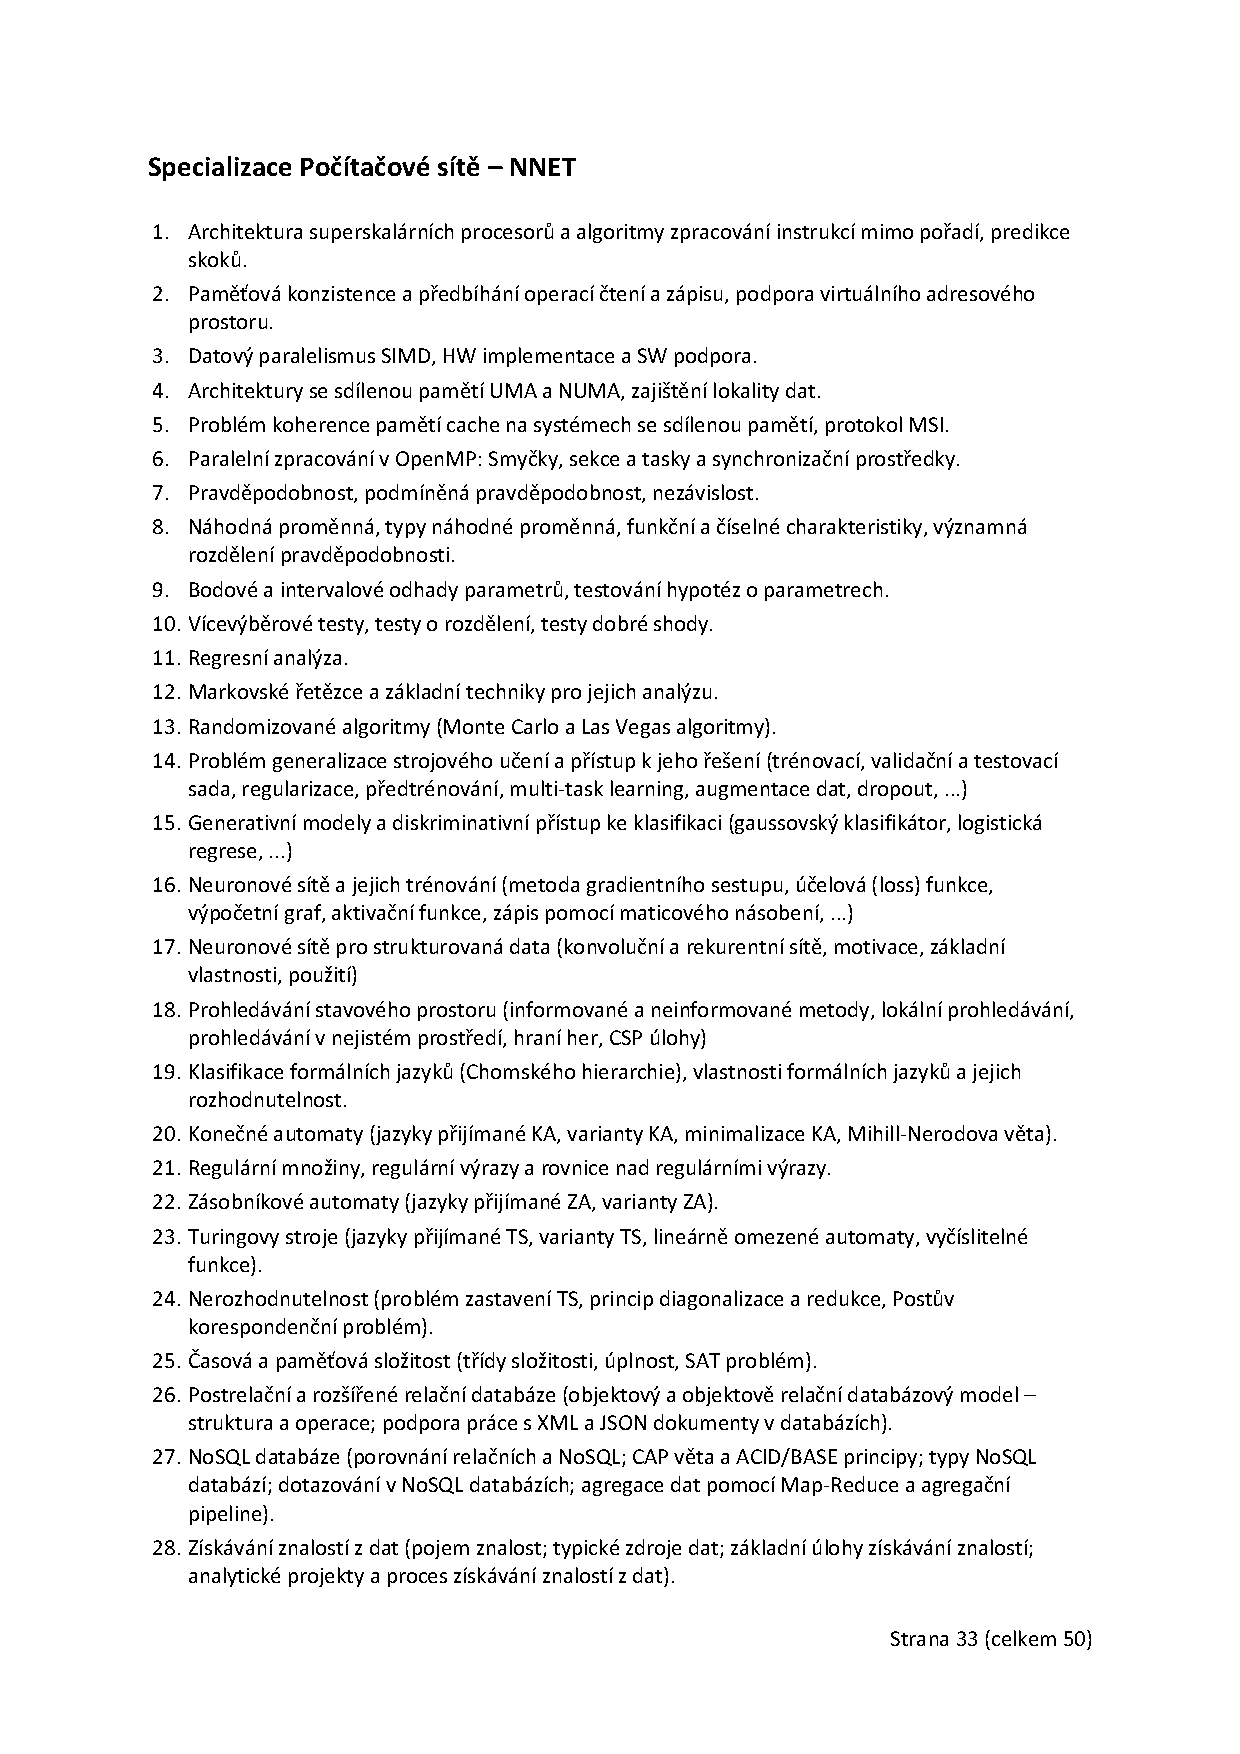
\includepdf[pages=-]{statnicovy_otazky_2022_nnet.pdf}

%%%%%%%%%%%%%%%%%%%%%%%%%%%%%%%%%%%%%%%%%%%%%%%%%%%%%%%%%%%%%%%%%%%%%%%%%%%%%%%%

\tableofcontents
\newpage

%%%%%%%%%%%%%%%%%%%%%%%%%%%%%%%%%%%%%%%%%%%%%%%%%%%%%%%%%%%%%%%%%%%%%%%%%%%%%%%%

% 44 - todo
% VUT FIT MITAI
% MSZ 2021/2022
% Author: Vladimir Dusek
% Login: xdusek27

%%%%%%%%%%%%%%%%%%%%%%%%%%%%%%%%%%%%%%%%%%%%%%%%%%%%%%%%%%%%%%%%%%%%%%%%%%%%%%%%

\chapter{BMS -- Bezdrátové lokální sítě (Wifi, Bluetooth).}

% Otazka MSZ 2020, 113 MSK
% [Ocenasek] Bezpecnost bezdratovych siti, chvili me nechal mluvit, tak jsem rekl neco k WEPu, pak uz to bylo stylem otazka odpoved. Zajimala ho proudova sifra WEPu, TKIP ve WPA, WPA enterprise a 802.1x, ale vetsinou chtel vedet spis veci obecneho charakteru, napr. jake jsou vyhody WPA enterprise oproti PSK a tak

%%%%%%%%%%%%%%%%%%%%%%%%%%%%%%%%%%%%%%%%%%%%%%%%%%%%%%%%%%%%%%%%%%%%%%%%%%%%%%%%

\section{Metadata}

\begin{compactitem}
    \item Předmět: Bezdrátové a mobilní sítě (BMS)
    \item Přednáška:
    \begin{compactitem}
        \item \todo{todo}
    \end{compactitem}
    \item Záznam:
    \begin{compactitem}
        \item \todo{todo}
    \end{compactitem}
\end{compactitem}

%%%%%%%%%%%%%%%%%%%%%%%%%%%%%%%%%%%%%%%%%%%%%%%%%%%%%%%%%%%%%%%%%%%%%%%%%%%%%%%%

\section{Úvod a kontext}

\todo{todo}

\newpage

% 45
% VUT FIT MITAI
% MSZ 2021/2022
% Author: Vladimir Dusek
% Login: xdusek27

%%%%%%%%%%%%%%%%%%%%%%%%%%%%%%%%%%%%%%%%%%%%%%%%%%%%%%%%%%%%%%%%%%%%%%%%%%%%%%%%

% Path to figures
\graphicspath{{gal/hledani_minimalni_kostry/figures}}

%%%%%%%%%%%%%%%%%%%%%%%%%%%%%%%%%%%%%%%%%%%%%%%%%%%%%%%%%%%%%%%%%%%%%%%%%%%%%%%%

\chapter{GAL -- Hledání minimální kostry obyčejného grafu (pojmy, stromy a kostry, Kruskalův algoritmus, Primův algoritmus).}

%%%%%%%%%%%%%%%%%%%%%%%%%%%%%%%%%%%%%%%%%%%%%%%%%%%%%%%%%%%%%%%%%%%%%%%%%%%%%%%%

\section{Zdroje}

\begin{compactitem}
    \item Předmět: Grafové algoritmy (GAL)
    \item Přednáška:
    \begin{compactitem}
        \item 5) Stromy, minimální kostry, Jarníkův a Borůvkův algoritmus.
        \item 6) Růst minimální kostry, algoritmy Kruskala a Prima.
    \end{compactitem}
    \item Záznam:
    \begin{compactitem}
        \item 2020-10-22
        \item 2020-10-29
    \end{compactitem}
\end{compactitem}

%%%%%%%%%%%%%%%%%%%%%%%%%%%%%%%%%%%%%%%%%%%%%%%%%%%%%%%%%%%%%%%%%%%%%%%%%%%%%%%%

\section{Úvod a kontext}

\paragraph*{Orientovaný graf} Orientovaný graf je dvojice $G = (V, E)$, kde $V$ je konečná množina uzlů a $E \subseteq V \times V$ je množina hran.

\paragraph*{Neorientovaný graf} Neorientovaný graf je dvojice $G = (V, E)$, kde $V$ je konečná množina uzlů a $E \subseteq \binom{V}{2}$ je množina hran. (Hrana je tedy dvouprvková množina, avšak běžně se držíme stejného značení jako u~orientovaných grafů a používáme dvojici.)

\paragraph*{Ohodnocený graf} Ohodnocený graf je takový graf, jehož každá hrana má přiřazenou nějakou hodnotu, typicky definovanou pomocí váhové funkce $w : E \mapsto \mathbb{R}$.

\paragraph*{Podgraf} Graf $G' = (V', E')$ je podgraf grafu $G = (V, E)$ jestliže $V' \subseteq V$ a $E' \subseteq E$.

\paragraph*{Sled} Posloupnost uzlů $\langle v_0, v_1, \dots, v_k \rangle$, kde $(v_{i-1}, v_i) \in E$ pro $i = 1, \dots, k$ se nazývá sled délky $k$ z~$v_0$ do $v_k$.

\paragraph*{Uzavřený sled} Sled $\langle v_0, v_1, \dots, v_k \rangle$ se nazývá uzavřený, pokud existuje hrana $(v_0, v_k)$.

\paragraph*{Dosažitelnost} Pokud existuje sled $s$ z~uzlu $u$ do uzlu $v$, říkáme, že $v$ je dosažitelný z~$u$ sledem $s$, značeno $u \xRightarrow{\text{s}} v$.

\paragraph*{Tah} Tah je sled ve kterém se neopakují hrany.

\paragraph*{Cesta} Cesta je sled ve kterém se neopakují uzly.

\paragraph*{Souvislý graf} Neorientovaný graf se nazývá souvislý, pokud mezi libovolnými dvěma uzly existuje cesta.

\paragraph*{Kružnice} Uzavřená cesta se nazývá kružnice.

\paragraph*{Cyklus} Orientovaná kružnice se nazývá cyklus (první a poslední uzel je shodný).

\paragraph*{Prostý graf} Orientovaný graf bez cyklů se nazývá prostý.

\paragraph*{Acyklický graf} Graf je bez cyklů, resp. kružnic, se nazývá acyklický.

\paragraph*{Strom} Graf, který je souvislý a acyklický, se nazývá strom.

\paragraph*{Kostra} Strom, který tvoří podgraf souvislého grafu na množině všech jeho vrcholů, se nazývá kostra (\textit{spanning tree}).

\paragraph*{Minimální kostra} Nechť $G = (V, E)$ je souvislý neorientovaný graf s~váhovou funkcí $w : E \mapsto \mathbb{R}$. Minimální kostra (\textit{MST, minimum spanning tree}) je strom $G' = (V, E')$, kde $E' \subseteq E$ a $$w(E') = \sum_{(u,v) \in T} w(u, v)$$ je minimální ze všech možných alternativních koster.

\paragraph*{Seznam sousedů} Seznam sousedů (\textit{Adj}, \textit{adjacency list}) je reprezentace grafu v~paměti. Jde o~preferovanou variantu pro řídké grafy~--~kde $m << n^2$. Pro každý uzel máme definovaný seznam jeho sousedů.

\paragraph*{Matice sousednosti} Matice sousednosti (\textit{adjacency matrix}) je reprezentace grafu v~paměti. Jde o~preferovanou variantu pro husté grafy~--~kde $m$ je skoro $n^2$.

\begin{figure}[H]
    \centering
    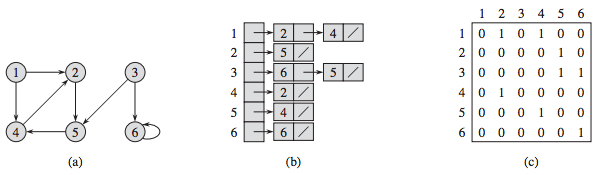
\includegraphics[width=1\linewidth]{graph_representations_example.png}
    \caption{Příklad reprezentace grafu pomocí seznamu sousedů a matice sousednosti.}
\end{figure}

%%%%%%%%%%%%%%%%%%%%%%%%%%%%%%%%%%%%%%%%%%%%%%%%%%%%%%%%%%%%%%%%%%%%%%%%%%%%%%%%

\section{Generický algoritmus}

Hledání minimální kostry je problém, který lze řešit algoritmy, které spadají do kategorie tzv. hladových (\textit{greedy}) deterministických algoritmů. Spočívají v~tom, že průběžně odhadují kostru přidáváním dalších hran a nikdy se nemusejí vracet (neprovádí se \textit{backtracking}). Generický algoritmus tvoří jakousi základní kostru pro další, už konkrétní, algoritmy.

\paragraph*{Řez} Nechť $G = (V, E)$ je graf. Řez grafu $G$ je dvojice $(S, V - S)$, kde $\emptyset \subseteq S \subseteq V$.

\paragraph*{Křížení} Hrana $(u, v) \in E$ kříží řez $(S, V - S)$, pokud jeden její konec je v~$S$ a druhý v~$V - S$.

\paragraph*{Respektování} Nechť $A \subseteq E$ je množina hran. Řez $(S, V - S)$ respektuje množinu hran $A$, pokud žádná hrana v~$A$ nekříží řez $(S, V - S)$.

\paragraph*{Lehkost} Nechť $(S, V - S)$ je řez a $B$ je množina hran, která ho kříží. Hrana z~množiny $B$ s~nejmenší hodnotou se nazývá lehká.

\paragraph*{Bezpečnost} Nechť $G = (V, E)$ je souvislý neorientovaný graf s~reálnou váhovou funkcí $w$. Nechť $A \subseteq E$ je součástí nějaké minimální kostry $G$. Nechť $(S, V - S)$ je řez, který respektuje $A$. Nechť $(u, v)$ je lehká hrana křížící $(S, V - S)$. Pak hrana $(u, v)$ je bezpečná pro $A$.

\bigskip\noindent\begin{minipage}{\linewidth}
\begin{lstlisting}[language=Python, caption={Generický algoritmus. Před každou iterací algoritmu je množina $A$ podmnožinou nějaké minimální kostry. Hrana $(u,v) \in E$ je bezpečná pro $A$, pokud $A \cup \{(u, v)\}$ je podmnožinou nějaké minimální kostry.}]
def generic_mst(G):
    # G je graf
    A = {} # A je mnozina hran rozpracovane minimalni kostry
    while netvori_kostru(A, G):
        for hrana in G.E:
            if je_bezpecna(A, hrana):
                A += {hrana}
    return A
\end{lstlisting}
\end{minipage}

\begin{figure}[H]
    \centering
    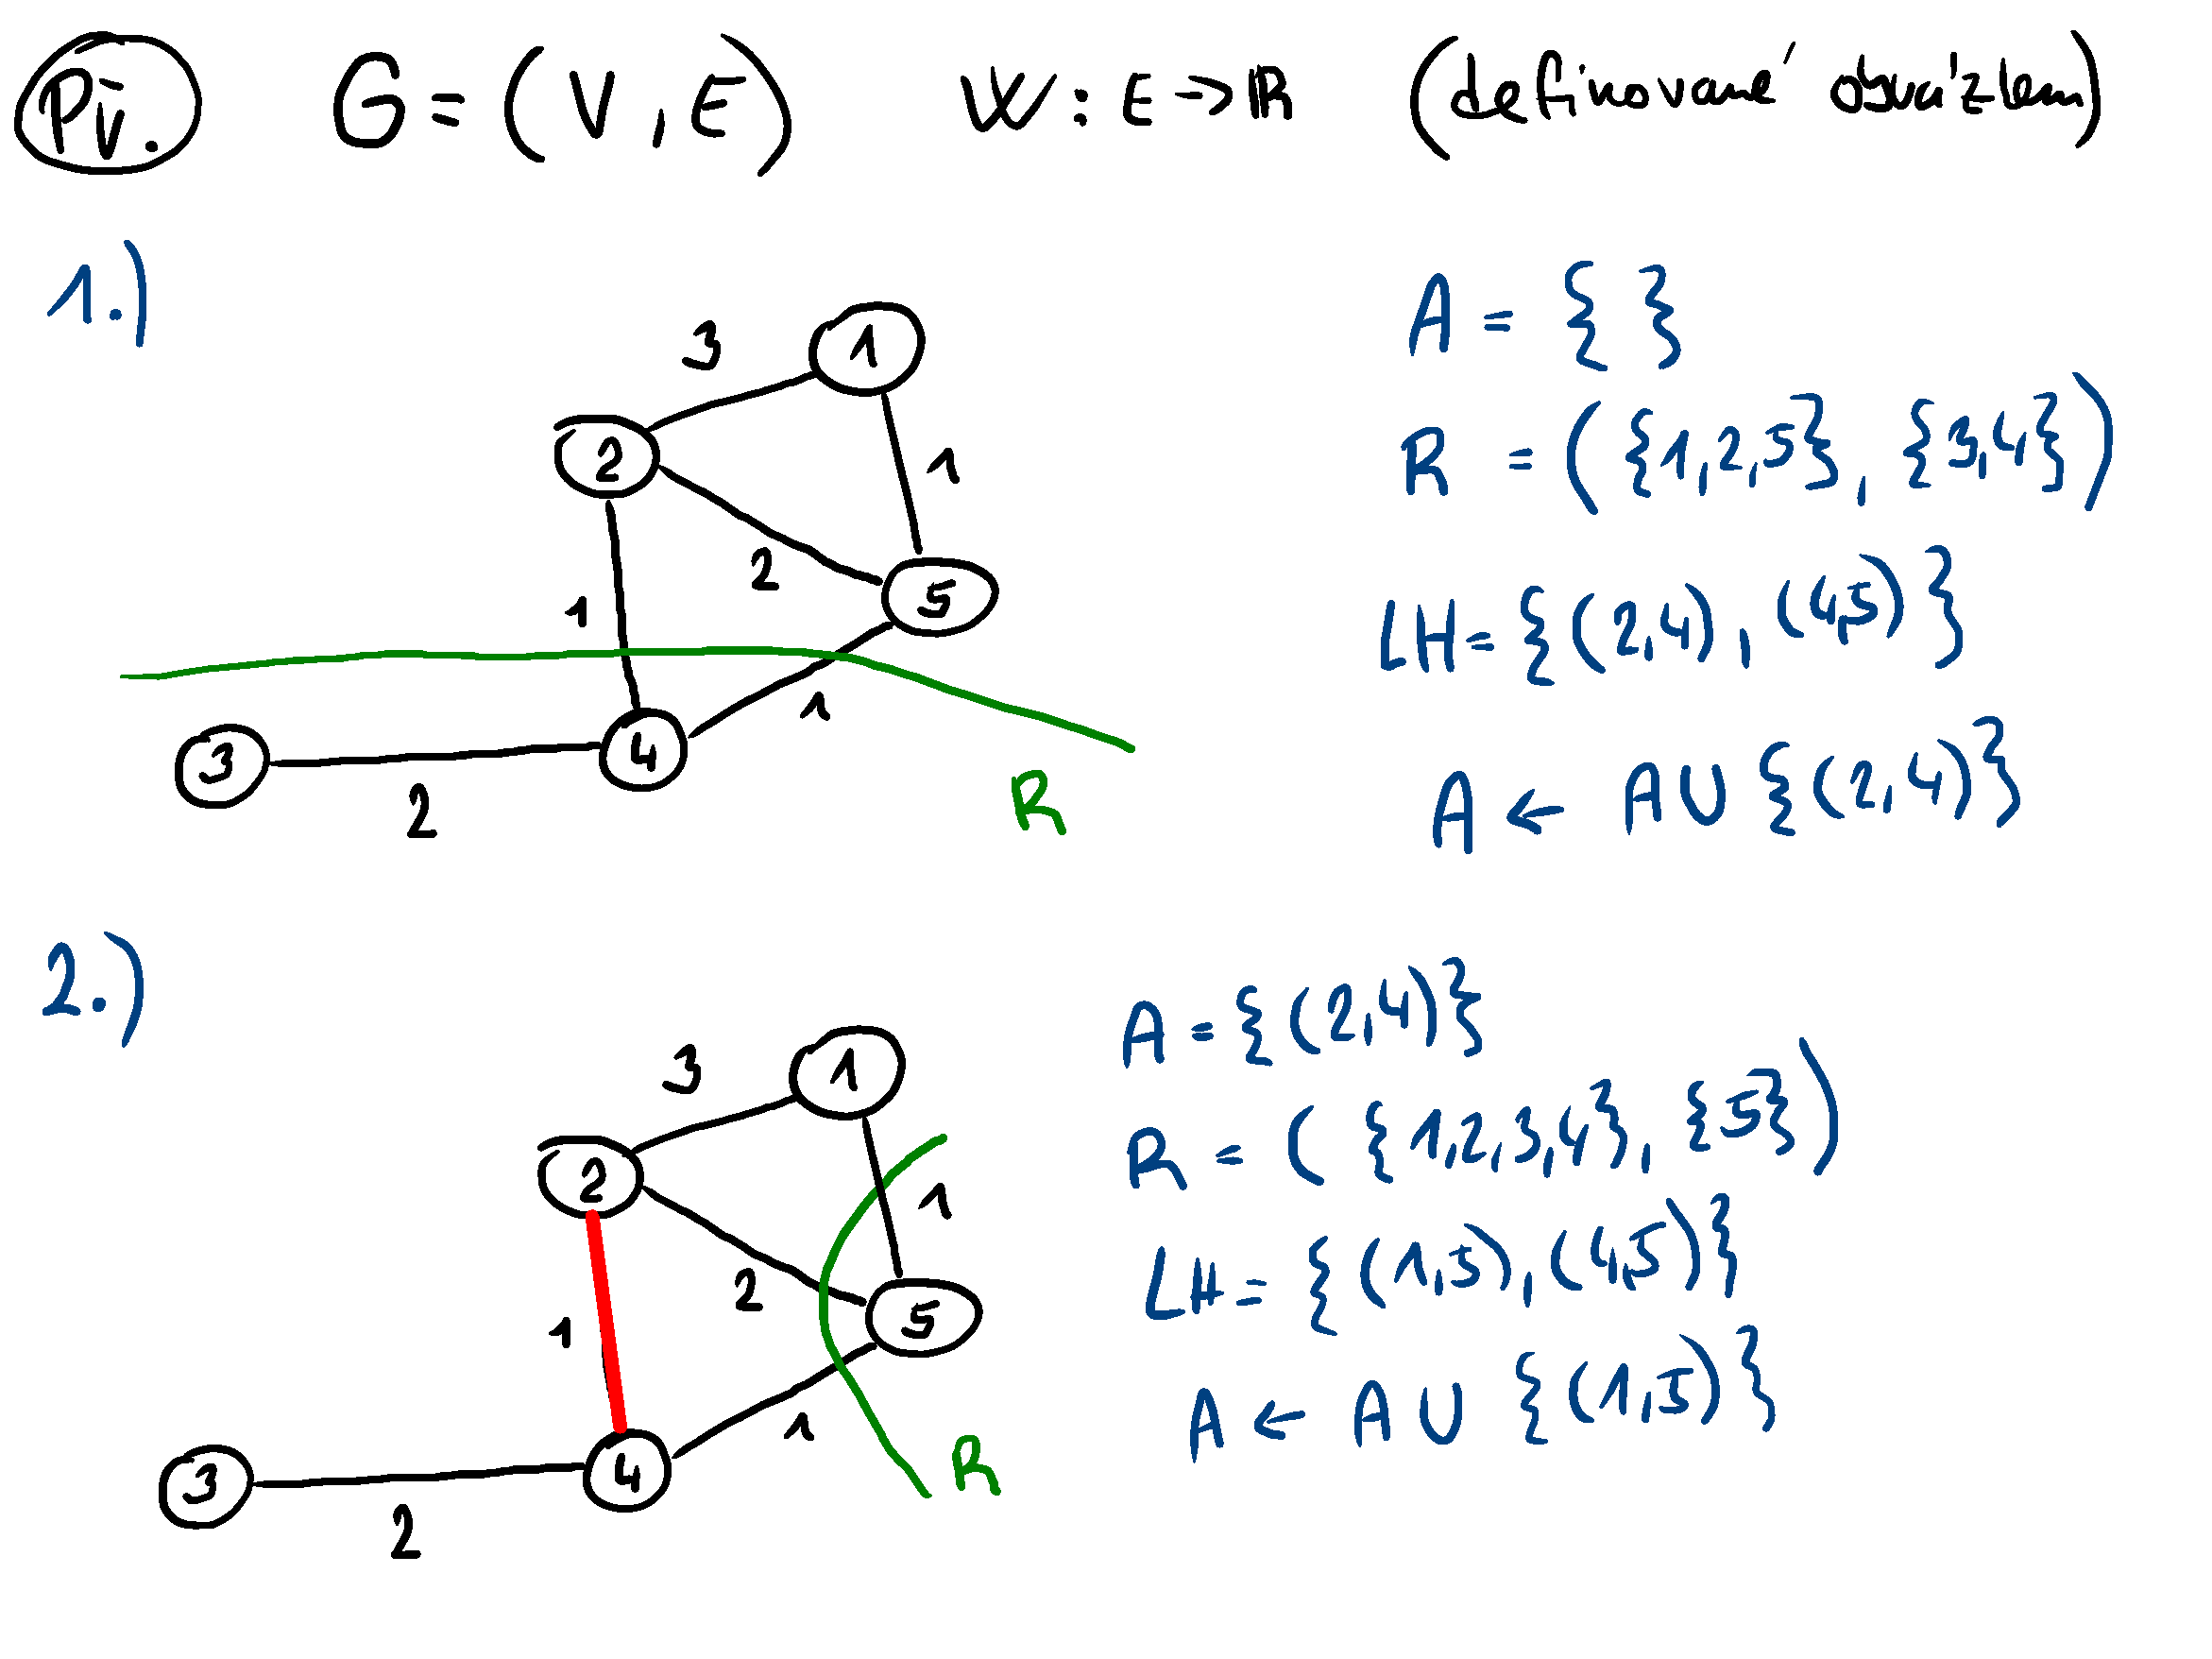
\includegraphics[width=0.9\linewidth]{03-minimalni-kostry-6.pdf}
    \caption{Příklad, část 1.}
\end{figure}

\begin{figure}[H]
    \centering
    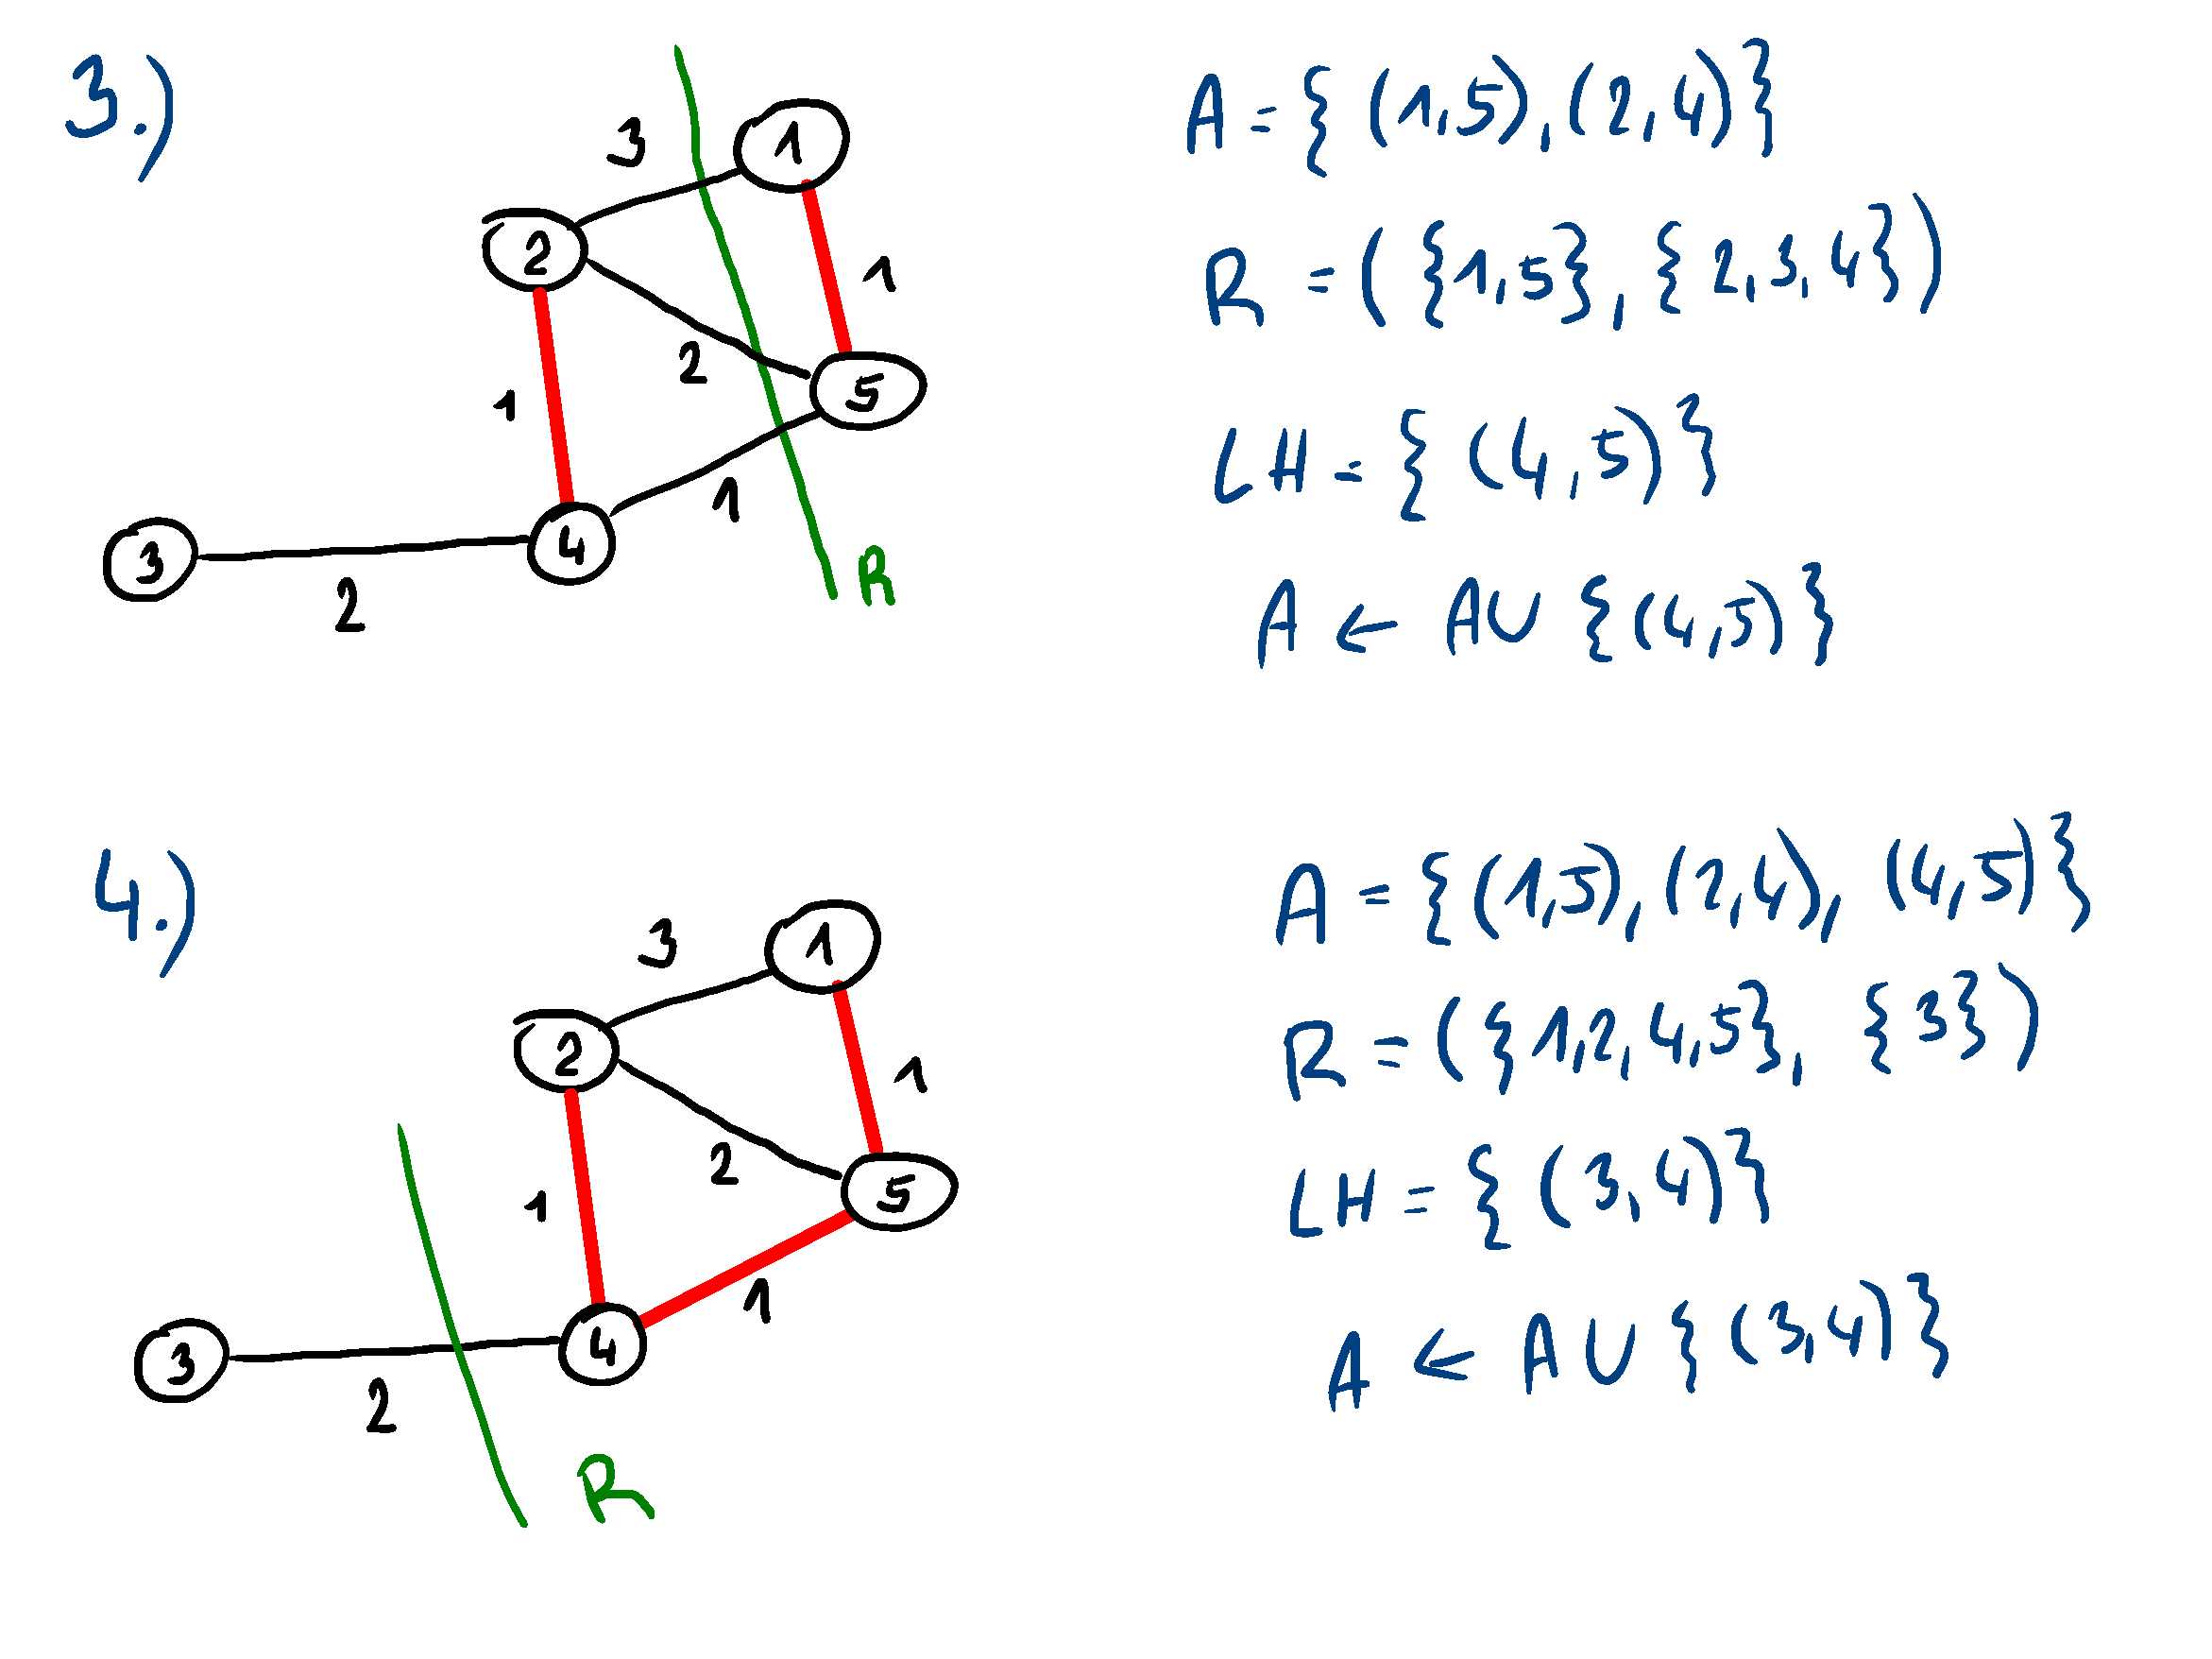
\includegraphics[width=0.9\linewidth]{03-minimalni-kostry-7.pdf}
    \caption{Příklad, část 2.}
\end{figure}

\begin{figure}[H]
    \centering
    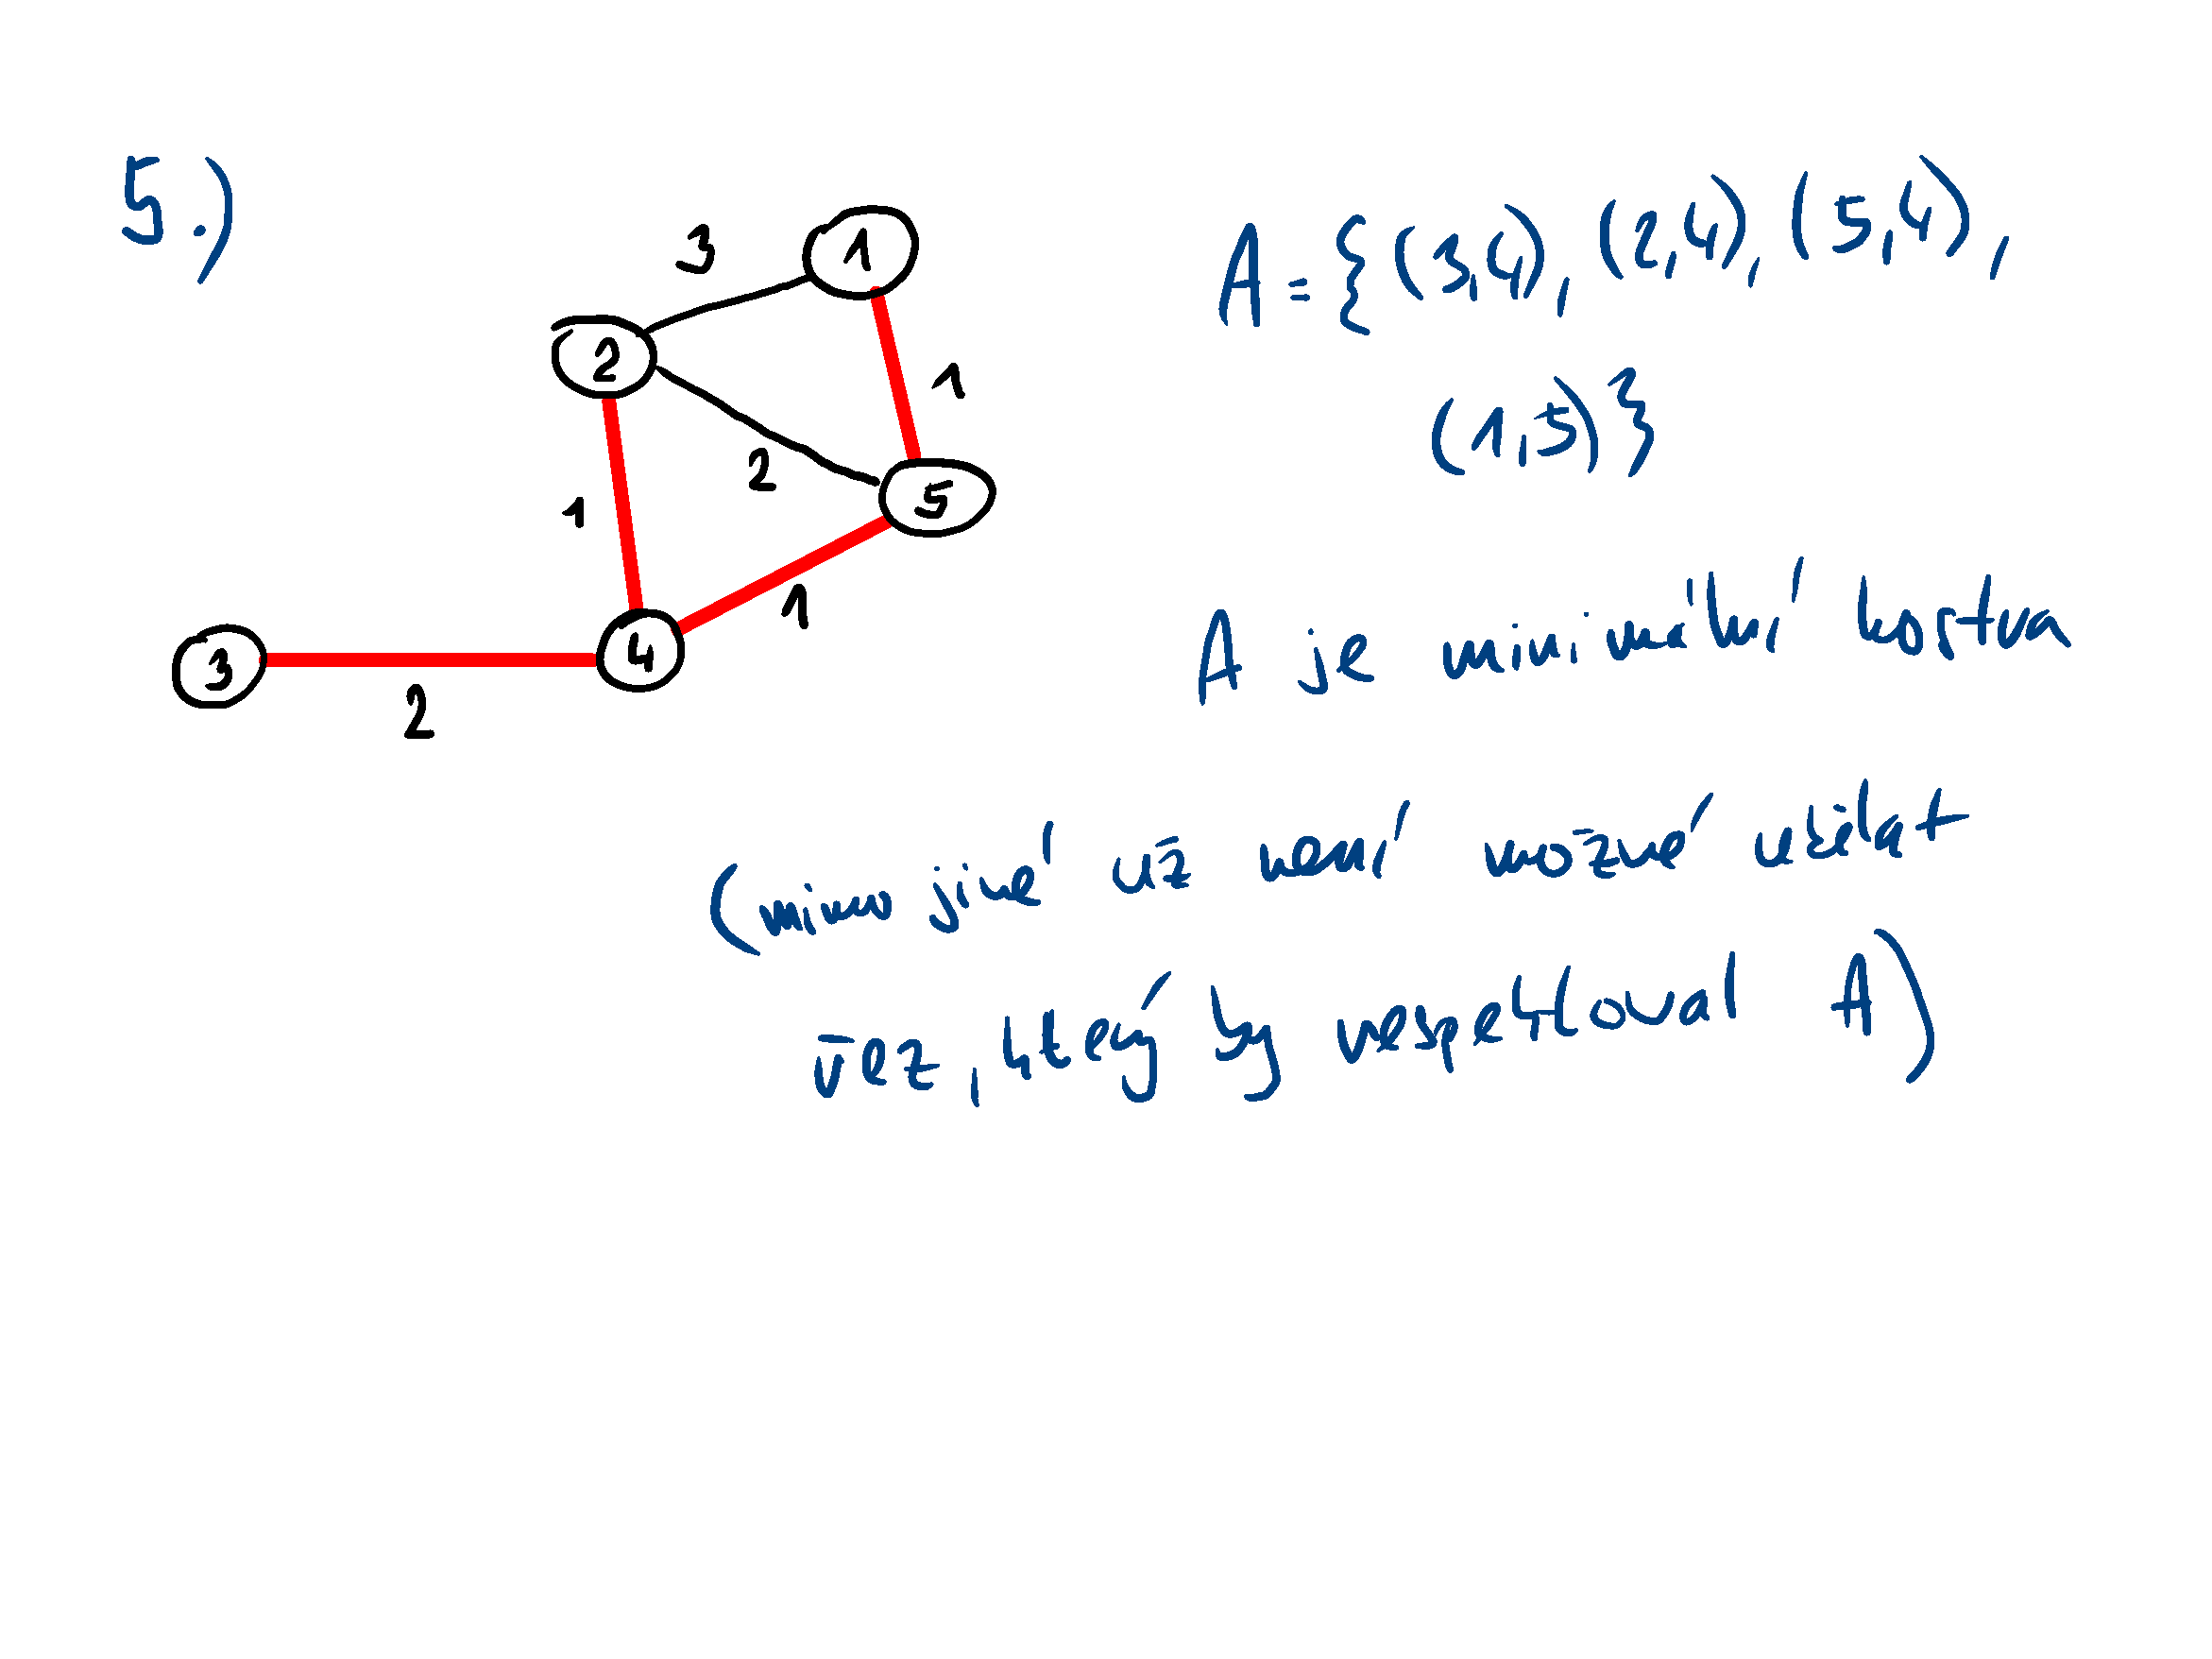
\includegraphics[width=0.9\linewidth]{03-minimalni-kostry-8.pdf}
    \caption{Příklad, část 3.}
\end{figure}

%%%%%%%%%%%%%%%%%%%%%%%%%%%%%%%%%%%%%%%%%%%%%%%%%%%%%%%%%%%%%%%%%%%%%%%%%%%%%%%%

\section{Kruskalův algoritmus}

Kruskalův a Primův algoritmus se liší v~tom, jakým způsobem vybírají bezpečnou hranu. Kruskalův algoritmus nahlíží na $A$ jako na les a hledá hranu s~nejmenším ohodnocením, která spojuje stromy v~lese. Na konci je $A$ jeden strom.

\bigskip\noindent\begin{minipage}{\linewidth}
\begin{lstlisting}[language=Python, caption={Kruskalův algoritmus. Funkce \texttt{make\_set(v)} vytvoří množinu obsahující $v$, \texttt{find\_set(v)} vrátí reprezentanta množiny ve které se nachází $v$, \texttt{union(u, v)} sjednotí dvě množiny obsahující $u$ a $v$.}]
def kruskal_mst(G):
    # G je graf

    # inicializace, kazdy uzel je ve sve mnozine
    A = {} # A je mnozina hran rozpracovane minimalni kostry
    for v in G.V:
        make_set(v)

    # seradit vzestupne podle w
    E = sort(G.E, G.w)

    for (u, v) in E:
        if find_set(u) != find_set(v):
            A += {(u, v)}
            union(u, v)

    return A
\end{lstlisting}
\end{minipage}

\subsection{Složitost}

\begin{compactitem}
    \item Řádek 5 -- $O(1)$
    \item Řádek 6-7 -- $n$-krát složitost $make\_set$ ($n$ je počet uzlů).
    \item Řádek 10 -- $O(m \cdot \log(m))$ ($m$ je počet hran).
    \item Řádky 12-15 -- Závisí na implementaci $find\_set$ a $union$.
    \begin{compactitem}
        \item Při implementaci seznamem s~heuristickou celkem: $O(m + n \cdot \log(n))$.
        \item Při stromové implementaci s~váhami a zkratkami celkem: $O((m+n) \cdot \alpha(n))$. Kde $\alpha$ je velmi pomalu rostoucí funkce ($\alpha \leq 4$).
    \end{compactitem}
    \item Pro souvislý graf platí $m > n$. Proto množinové operace stojí $O(m \cdot \alpha(n))$. Jelikož $\alpha(n) = O(\log(n)) = O(\log(m))$, tak celková složitost je $O(m \cdot \log(m))$.
    \item Dále platí $m < n^2$, pak $\log(m) = O(\log(n))$, proto celkem: $O(m \cdot \log(n))$.
\end{compactitem}

\subsection{Příklad}

\begin{figure}[H]
    \centering
    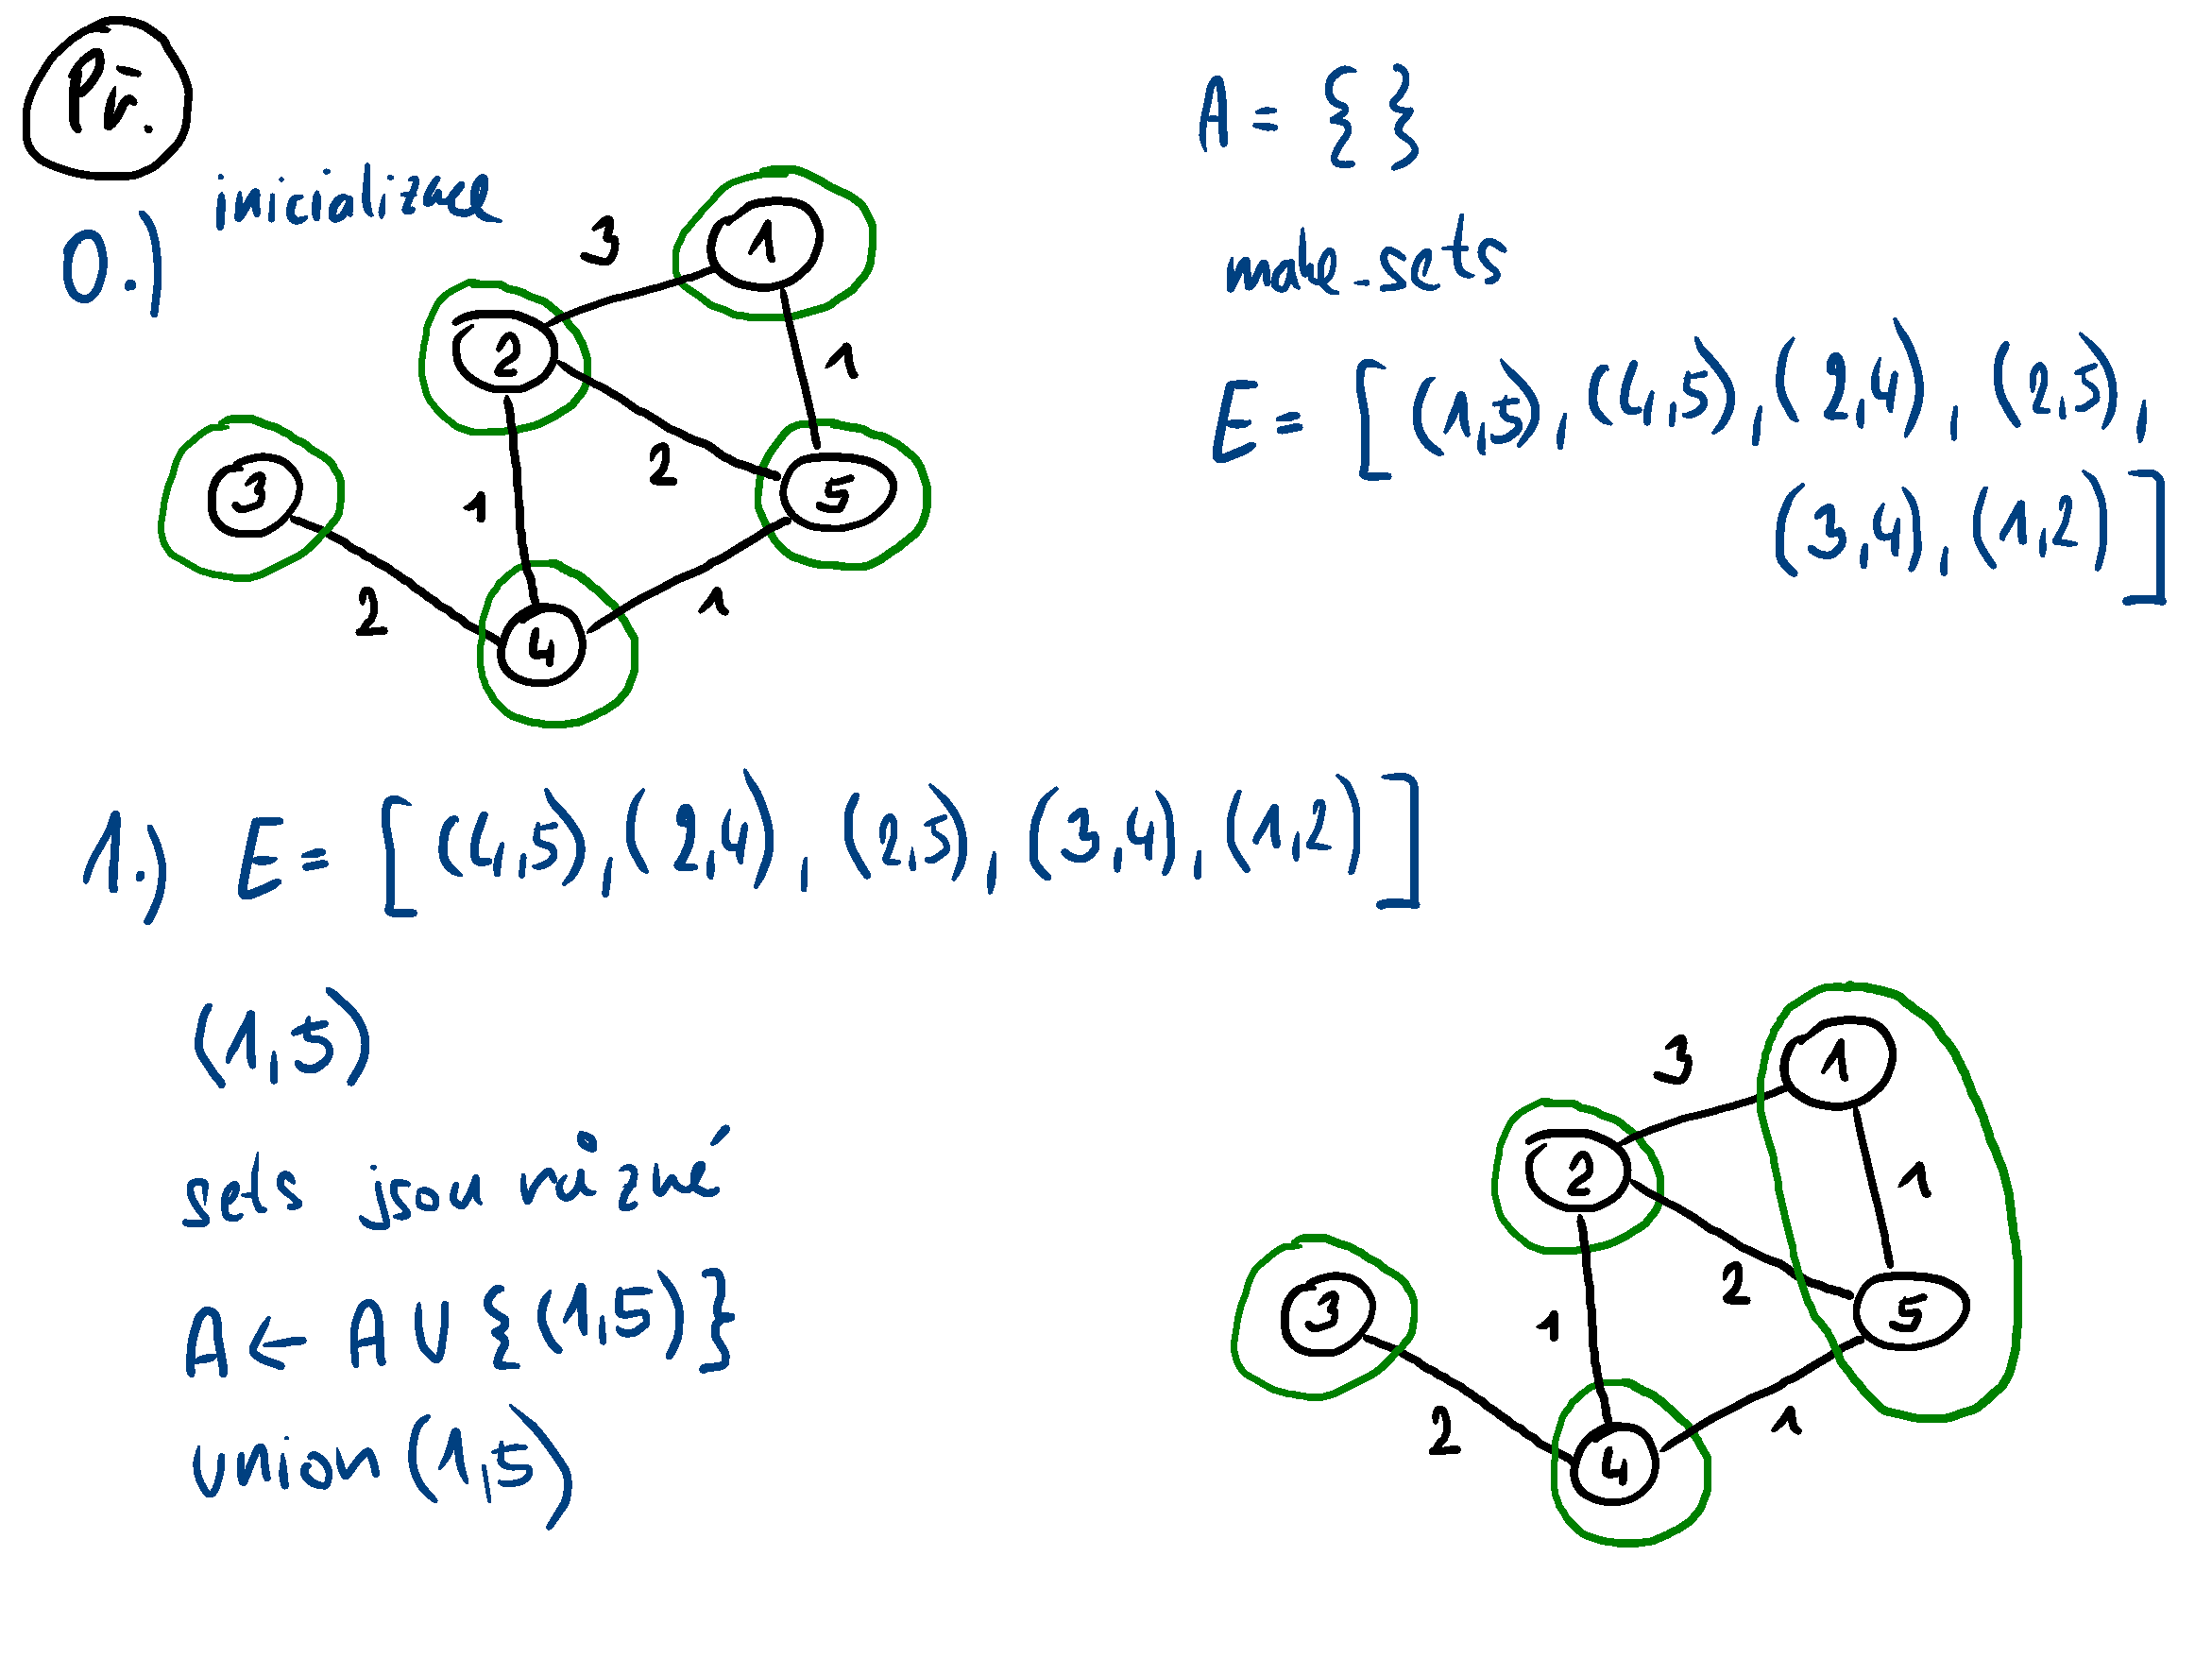
\includegraphics[width=0.9\linewidth]{03-minimalni-kostry-11.pdf}
    \caption{Příklad, část 1.}
\end{figure}

\begin{figure}[H]
    \centering
    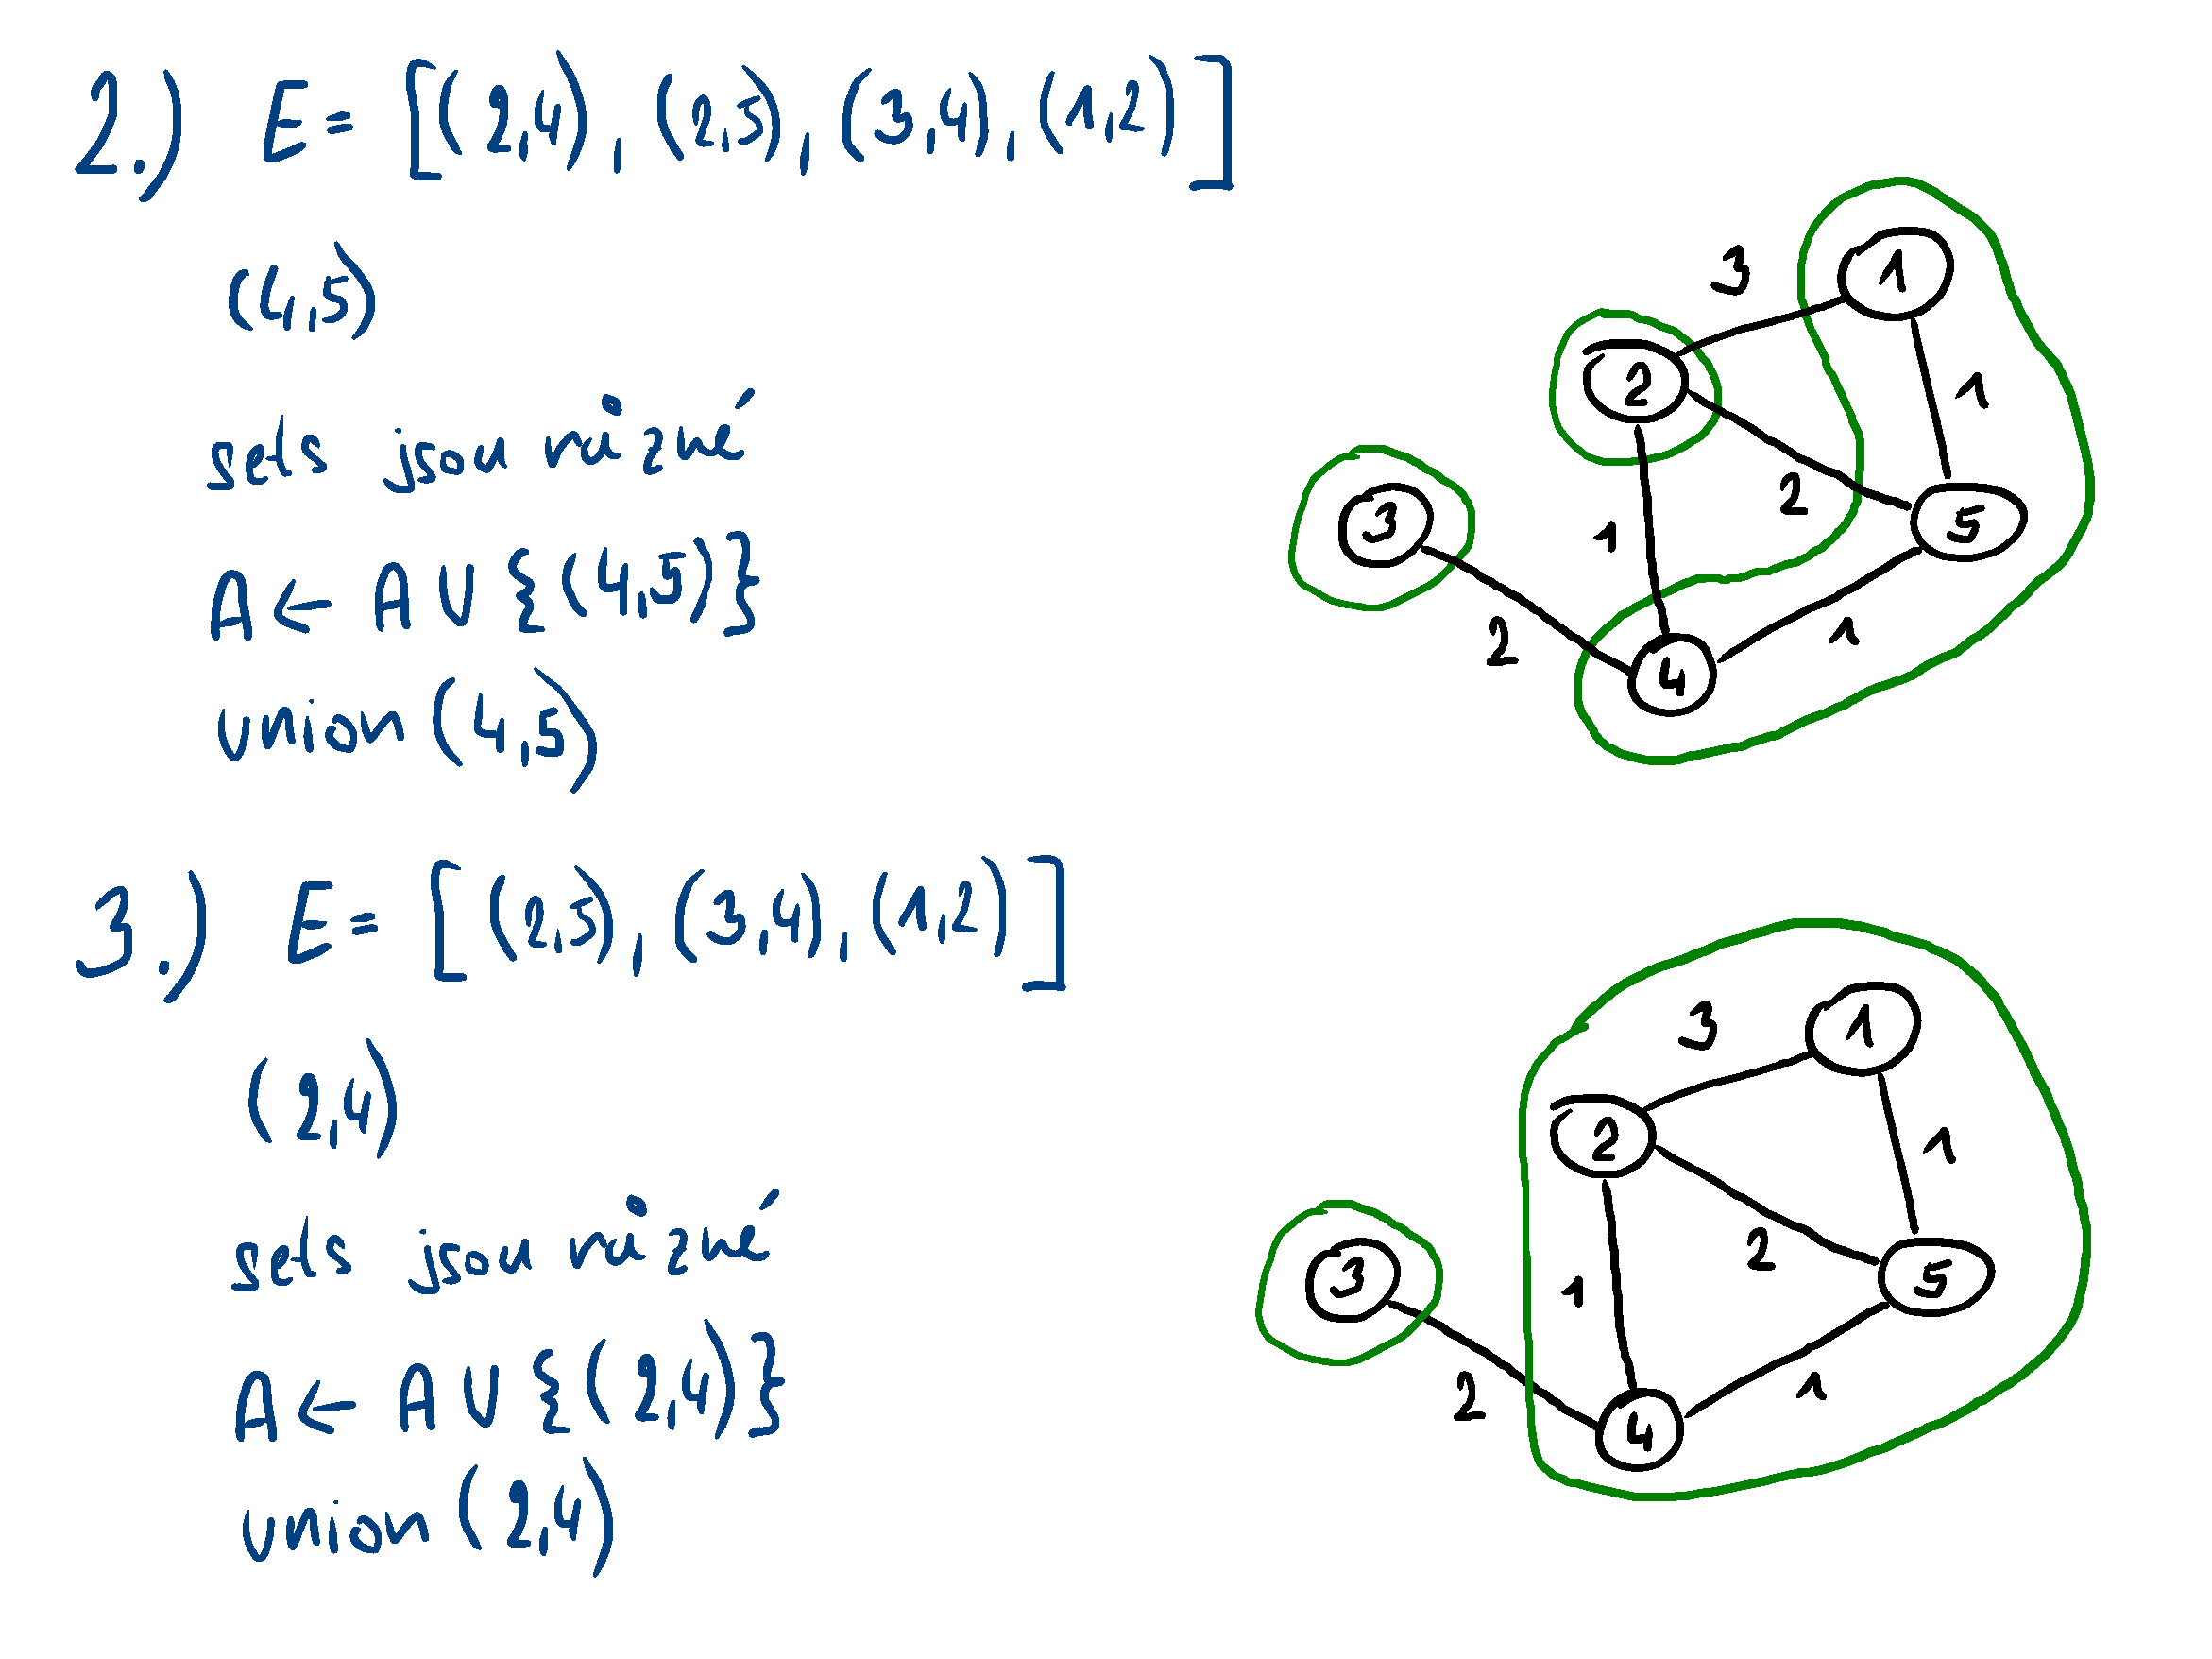
\includegraphics[width=0.9\linewidth]{03-minimalni-kostry-12.pdf}
    \caption{Příklad, část 2.}
\end{figure}

\begin{figure}[H]
    \centering
    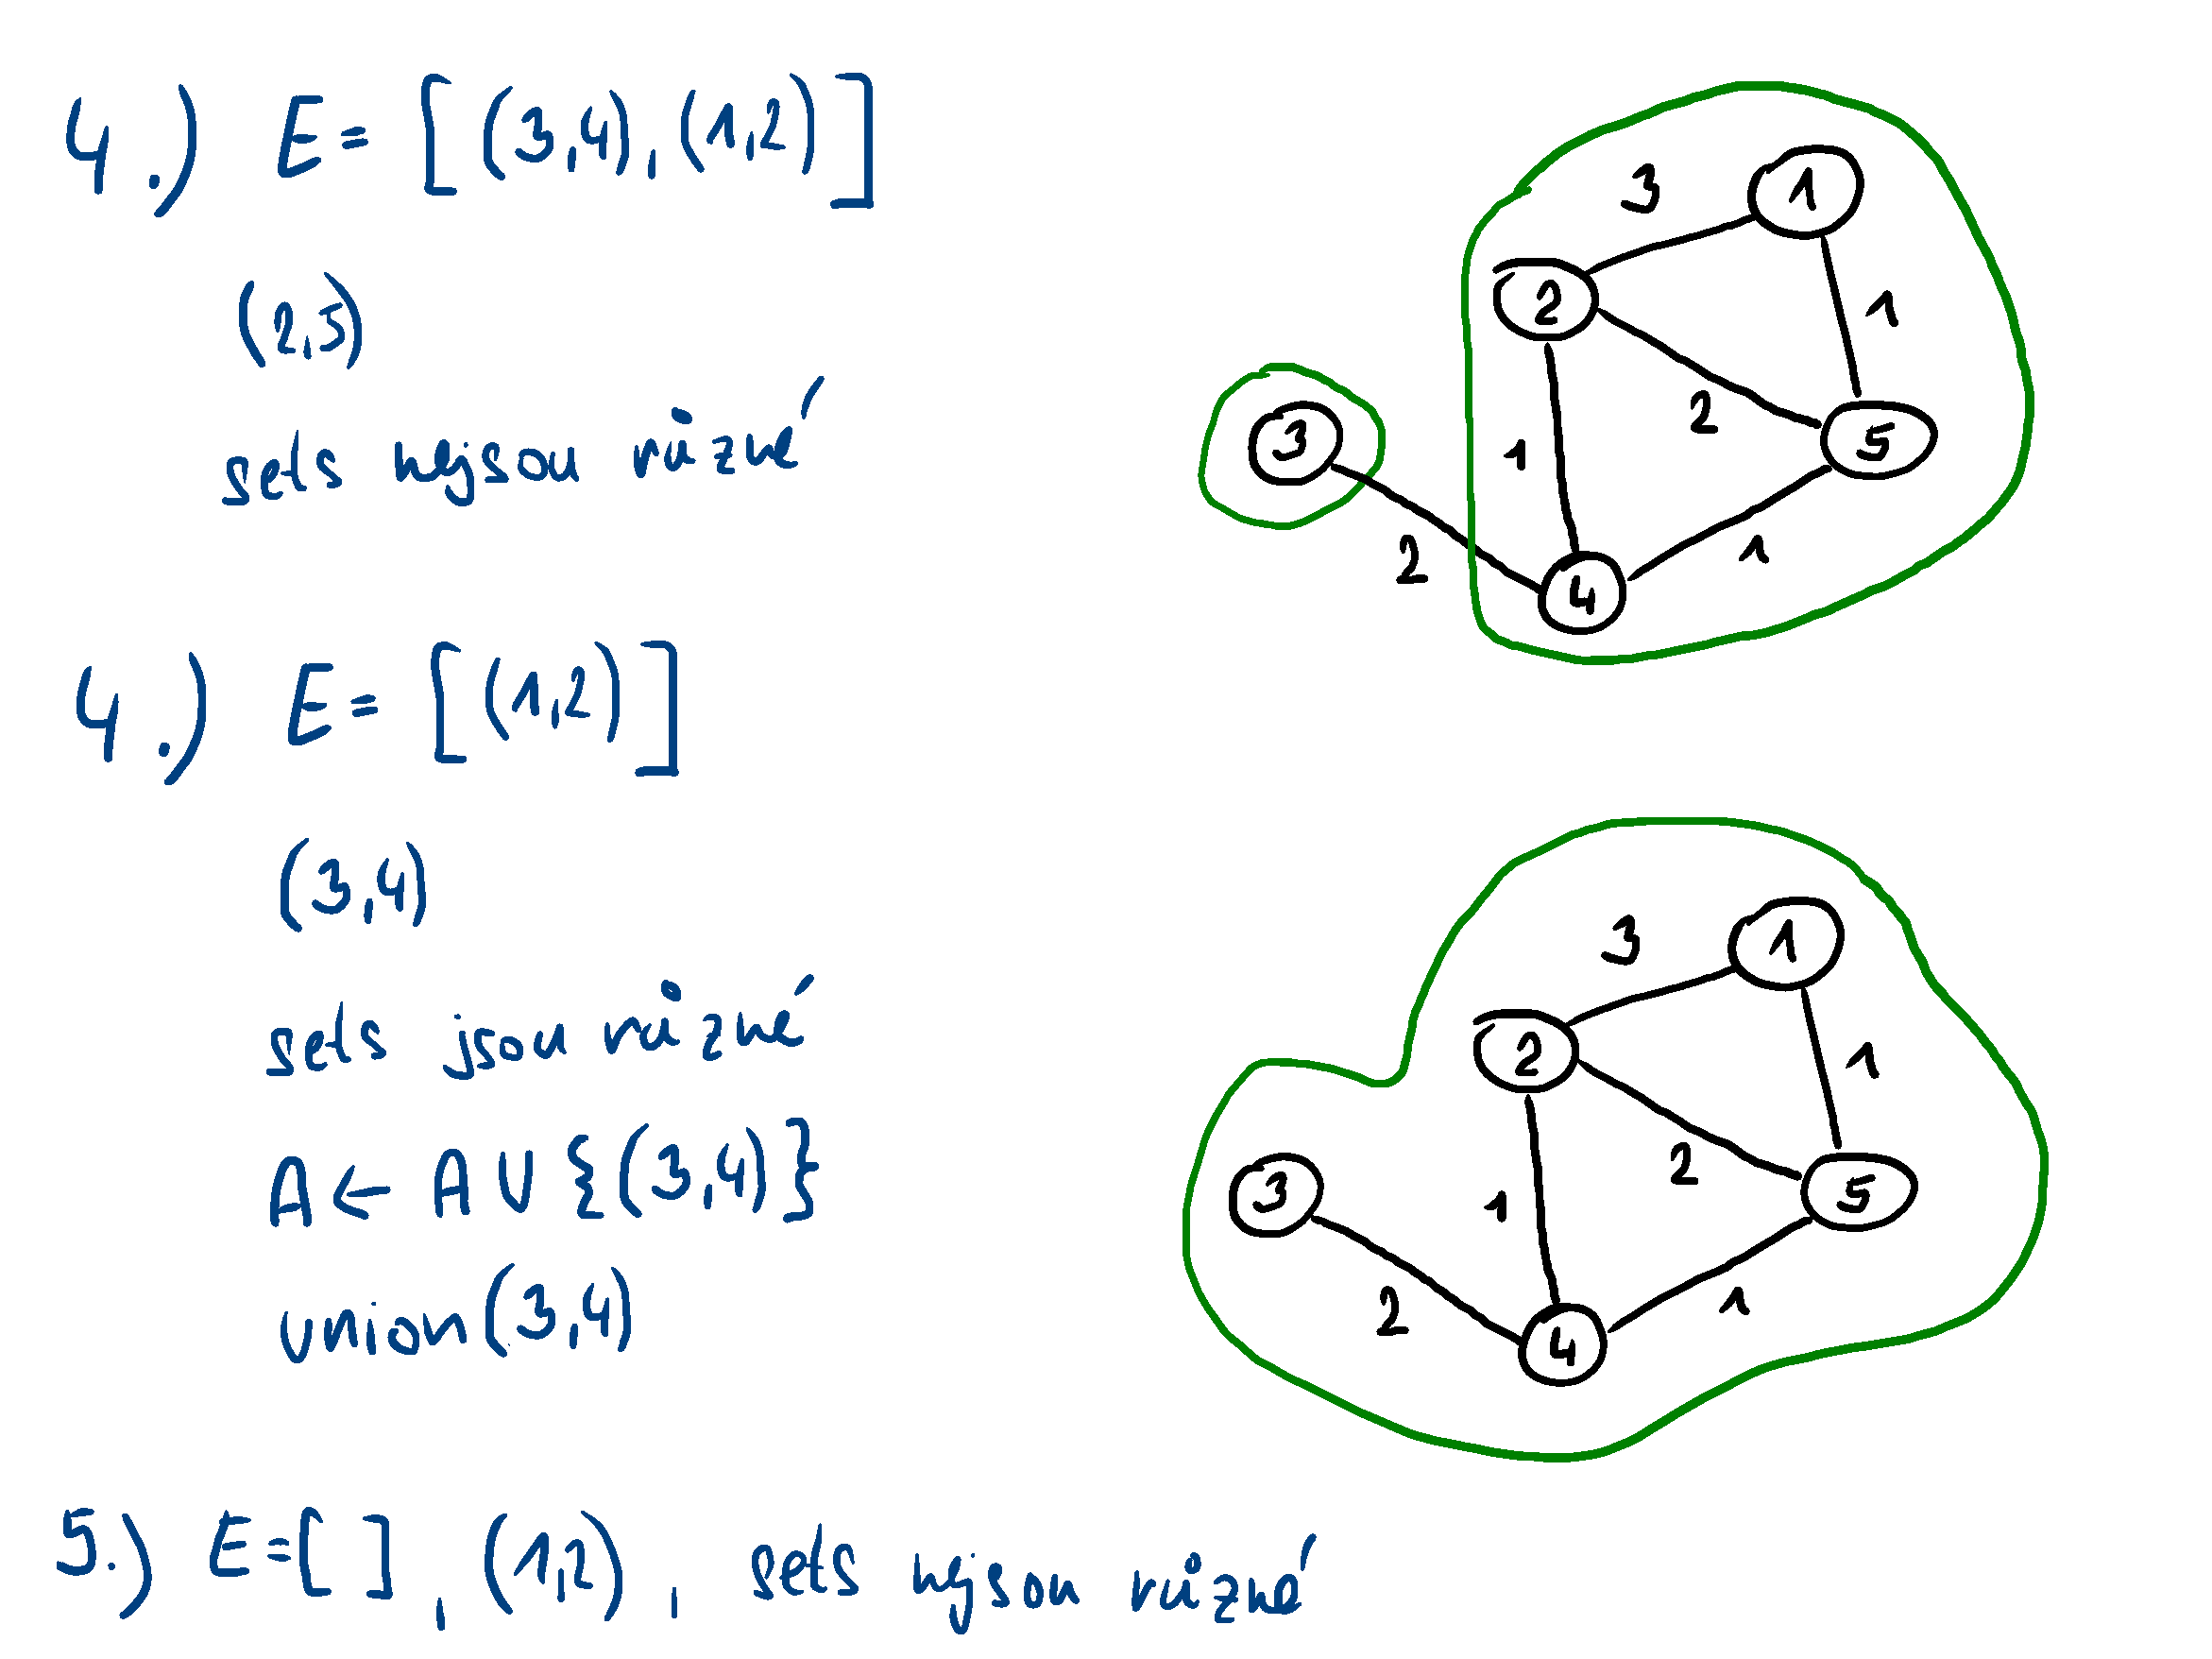
\includegraphics[width=0.9\linewidth]{03-minimalni-kostry-13.pdf}
    \caption{Příklad, část 3.}
\end{figure}

%%%%%%%%%%%%%%%%%%%%%%%%%%%%%%%%%%%%%%%%%%%%%%%%%%%%%%%%%%%%%%%%%%%%%%%%%%%%%%%%

\section{Primův-Jarníkův algoritmus}

Primův algoritmus buduje tzv. $A$ strom. Má zadaný určitý uzel, ze kterého hledá nejbližší další uzel, který by připojil. A~pak další a další.

\bigskip\noindent\begin{minipage}{\linewidth}
\begin{lstlisting}[language=Python, caption={Primův algoritmus.}]
def prim_mst(G, r):
    # G je graf
    # r je vychozi uzel

    for u in G.V:
        key[u] = INF # pole cen prechodu, kolik stoji prechod do vrcholu na indexu
        pi[u] = NULL # pole predchudcu, kdo je predchudce vrcholu na indexu

    key[r] = 0
    Q = Queue(G.V) # prioritni fronta uzlu

    while not Q.empty():
        u = Q.extract_min(key) # vrati prvek z Q s nejmensi hodnotou v key

        # pro vsechny sousedy uzlu u (Adj je seznam sousedu)
        for v in Adj[u]:
            # pokud je levnejsi cesta a jeste to neni prozkoumany uzel
            if v in Q and w(u, v) < key(v):
                pi[v] = u key[v] = w(u, v)
                Q.decrease_key(key) # aktualizace prioritni fronty

    return pi
\end{lstlisting}
\end{minipage}

\subsection{Složitost}

\begin{compactitem}
    \item Řádky 5-10 -- $O(n)$ za použití binární haldy ($n$ je počet uzlů).
    \item Řádky 12-13 -- While cyklus se provede n-krát a protože \textit{extract\_min} stojí $O(\log(n))$, tak je celková složitost $O(n \cdot \log(n))$.
    \item Řádek 16 -- For cyklus se provede $O(m)$ krát, protože dálka všech seznamů sousedů je dohromady $2m$ ($m$ je počet hran).
    \item Řádek 18-20 -- $O(1)$.
    \item Řádek 21 -- $O(\log(n))$.
    \item Jelikož $m > n$, tak celkem $O(n \cdot \log(n) + m \cdot \log(n)) = O(m \cdot \log(n))$.
\end{compactitem}

\subsection{Příklad}

\begin{figure}[H]
    \centering
    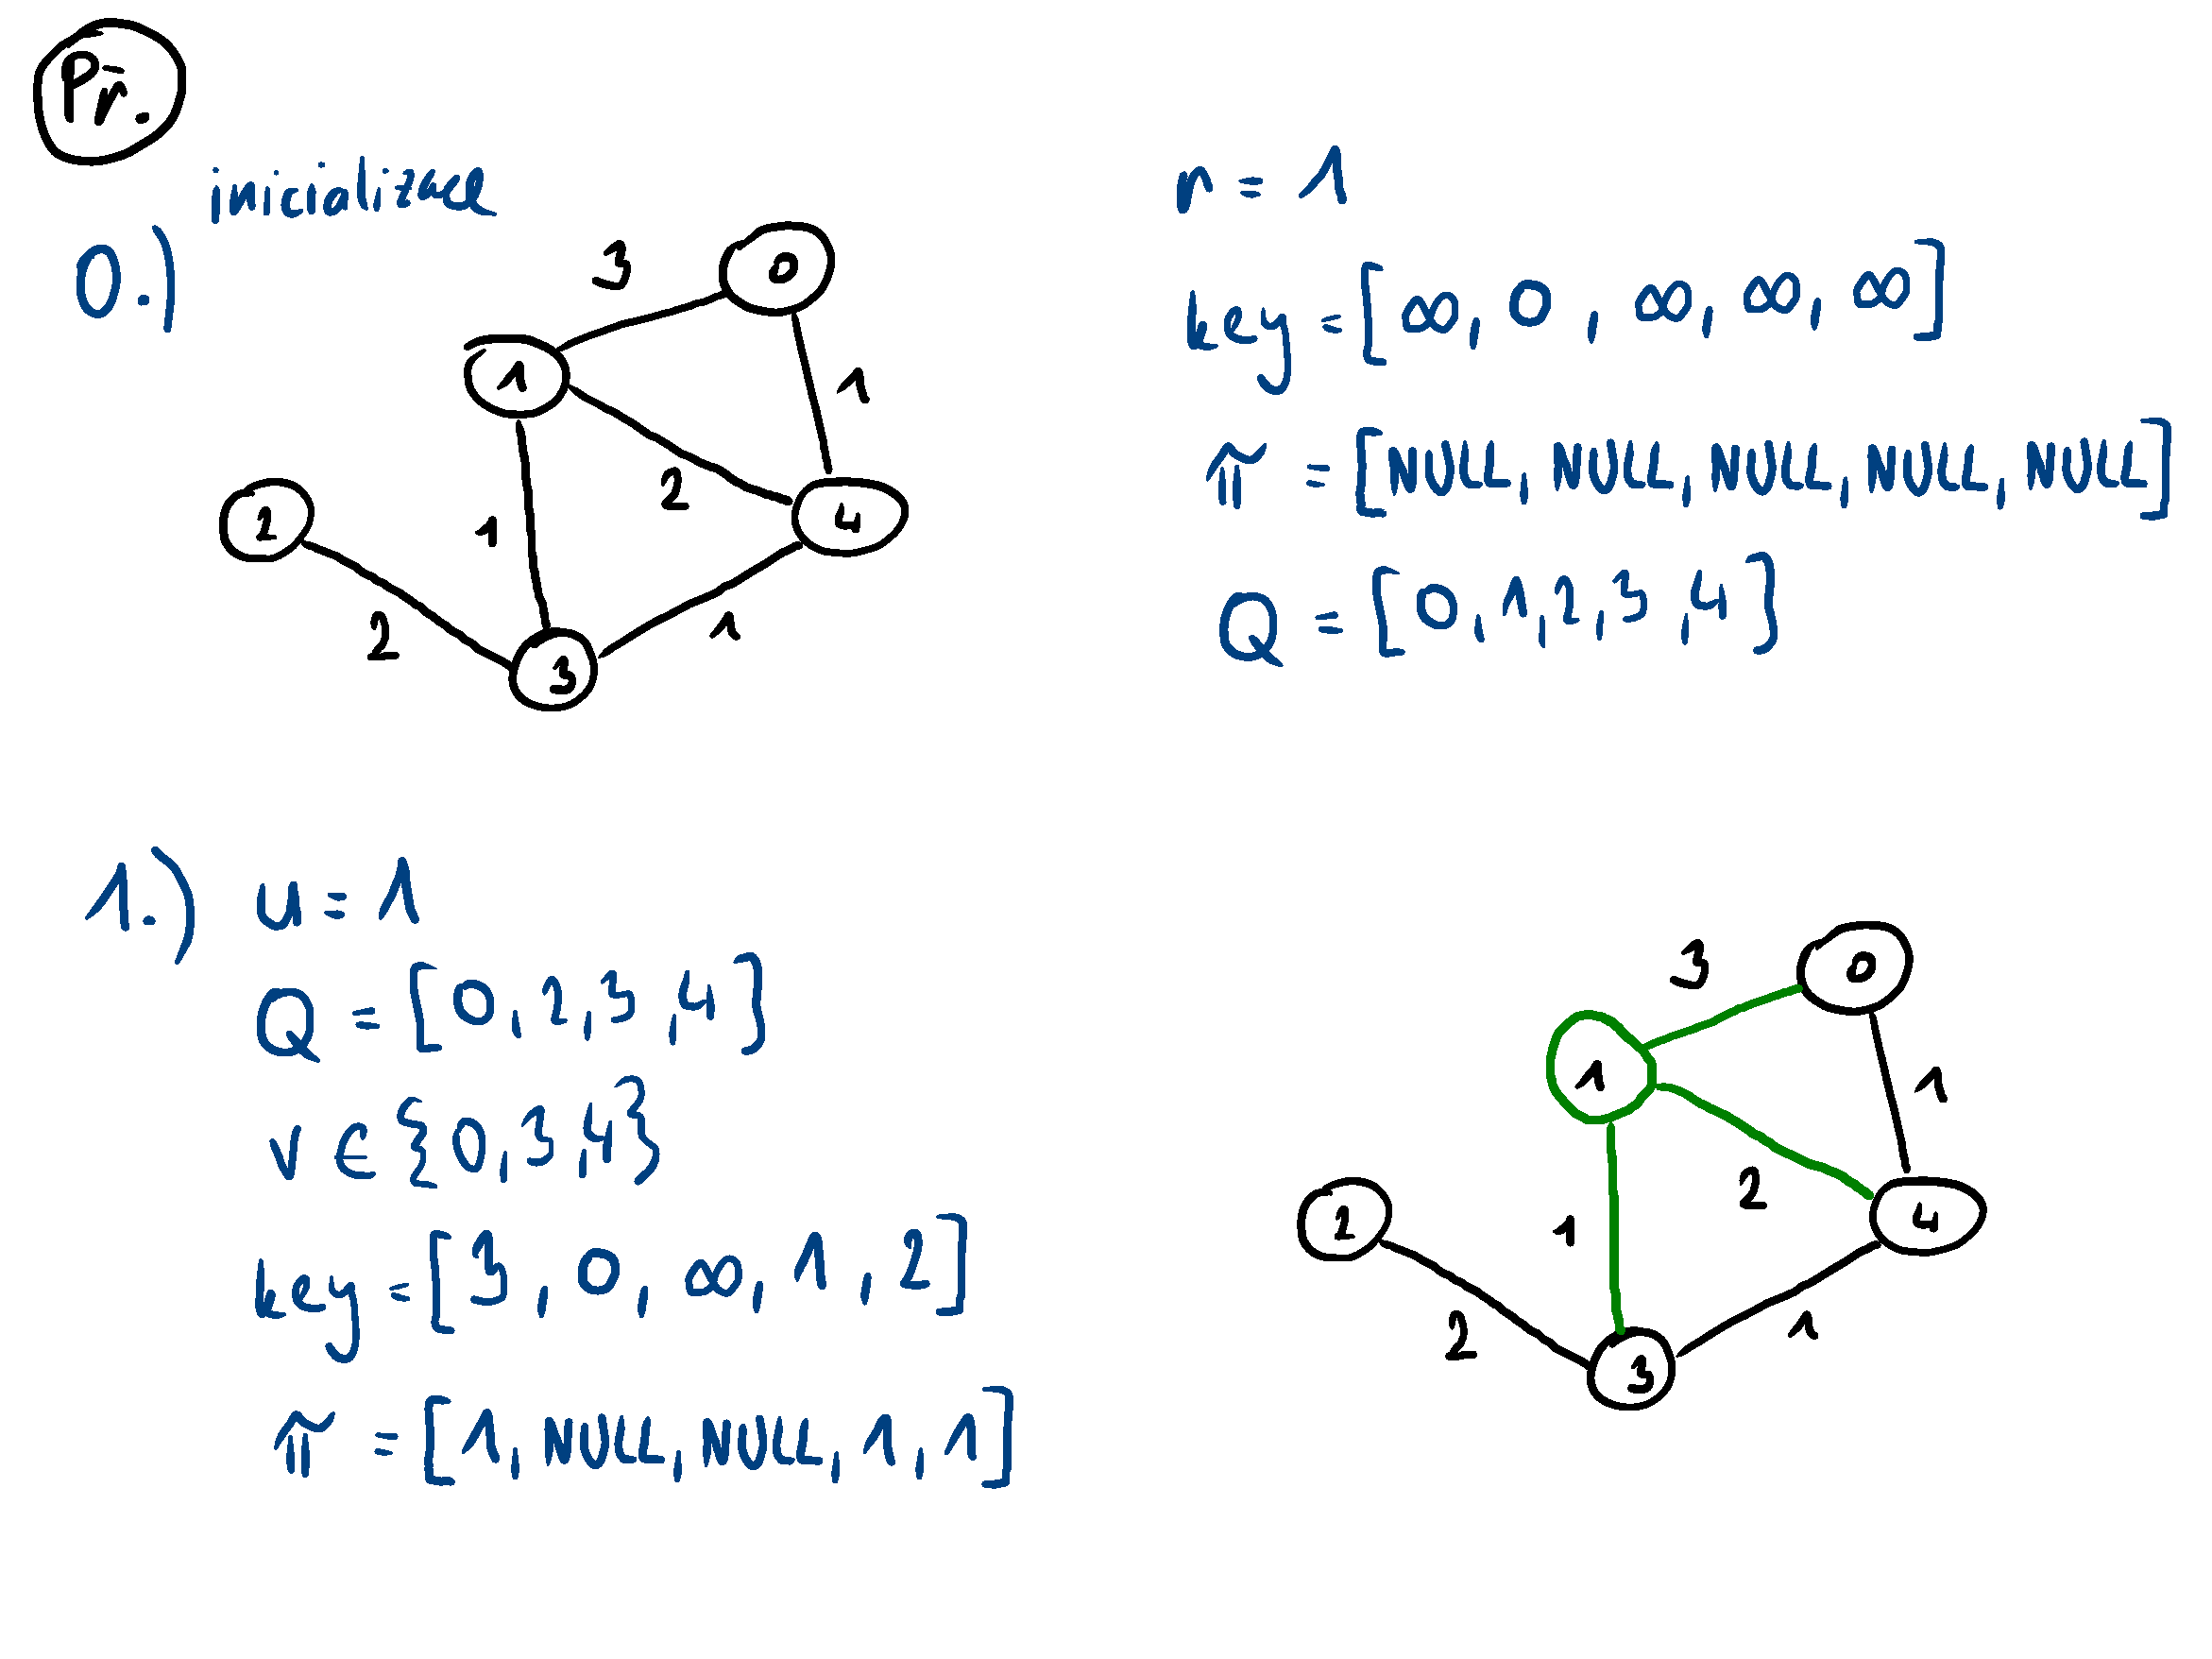
\includegraphics[width=0.9\linewidth]{03-minimalni-kostry-16.pdf}
    \caption{Příklad, část 1.}
\end{figure}

\begin{figure}[H]
    \centering
    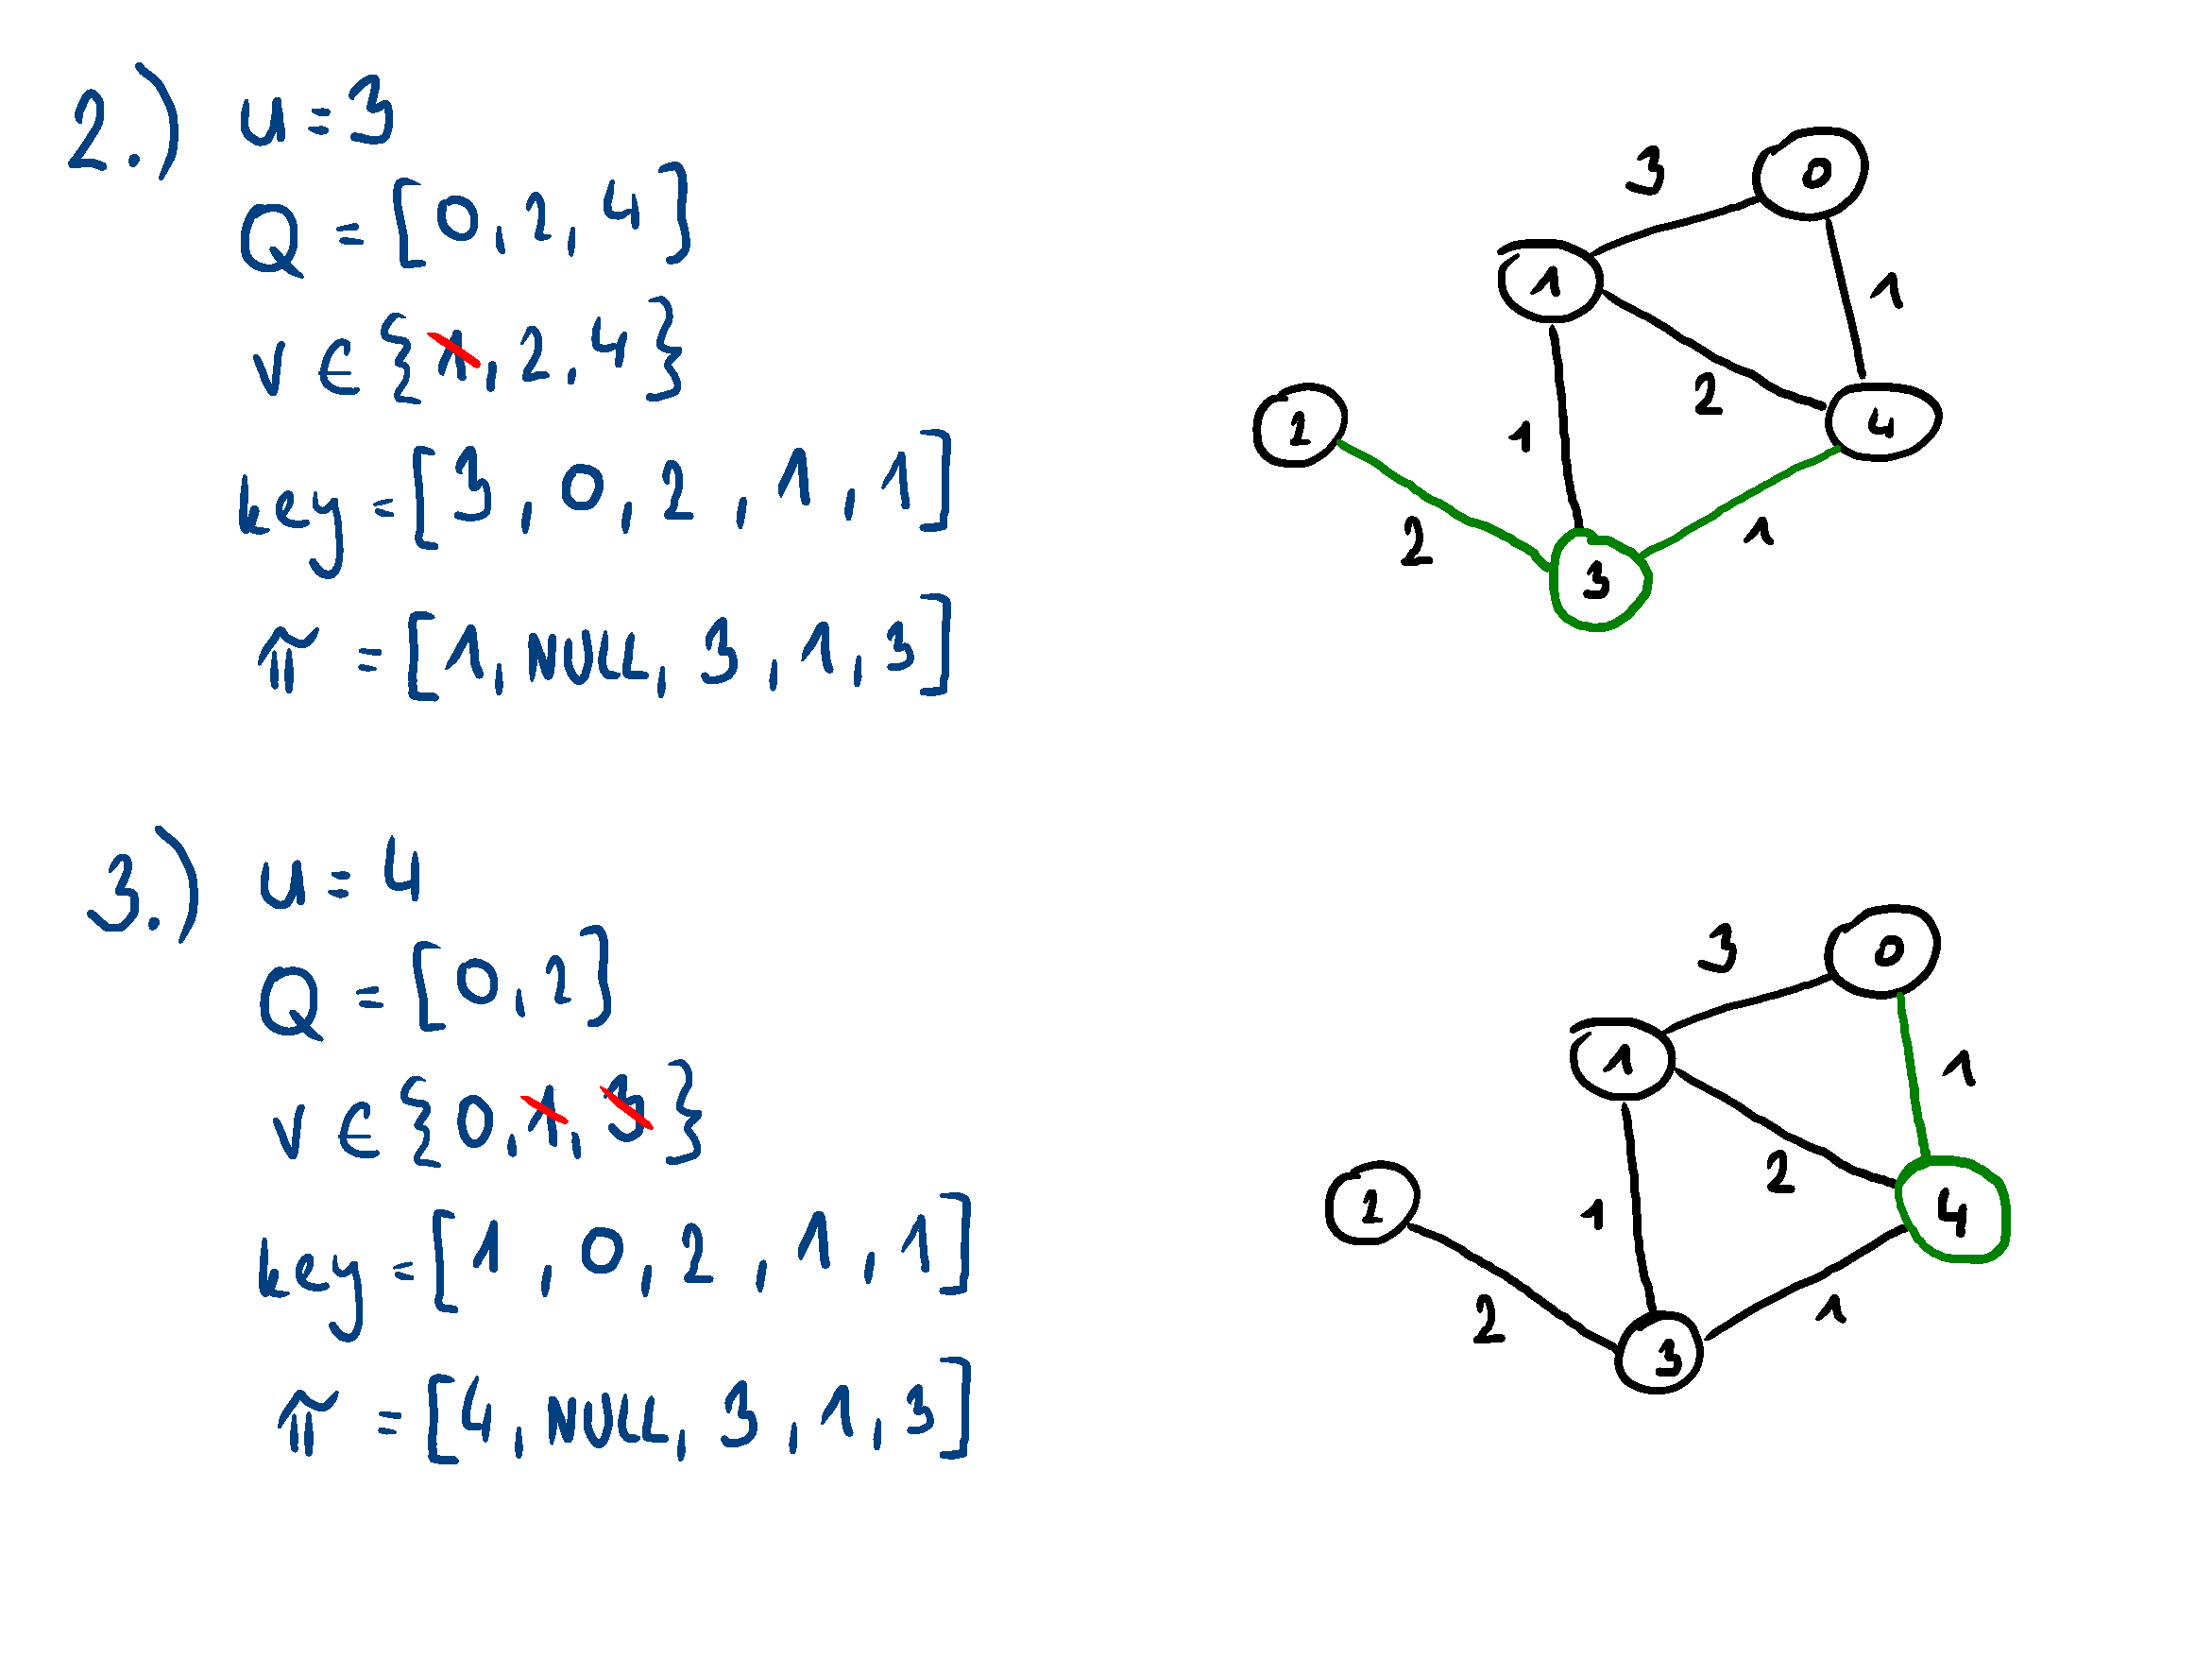
\includegraphics[width=0.9\linewidth]{03-minimalni-kostry-17.pdf}
    \caption{Příklad, část 2.}
\end{figure}

\begin{figure}[H]
    \centering
    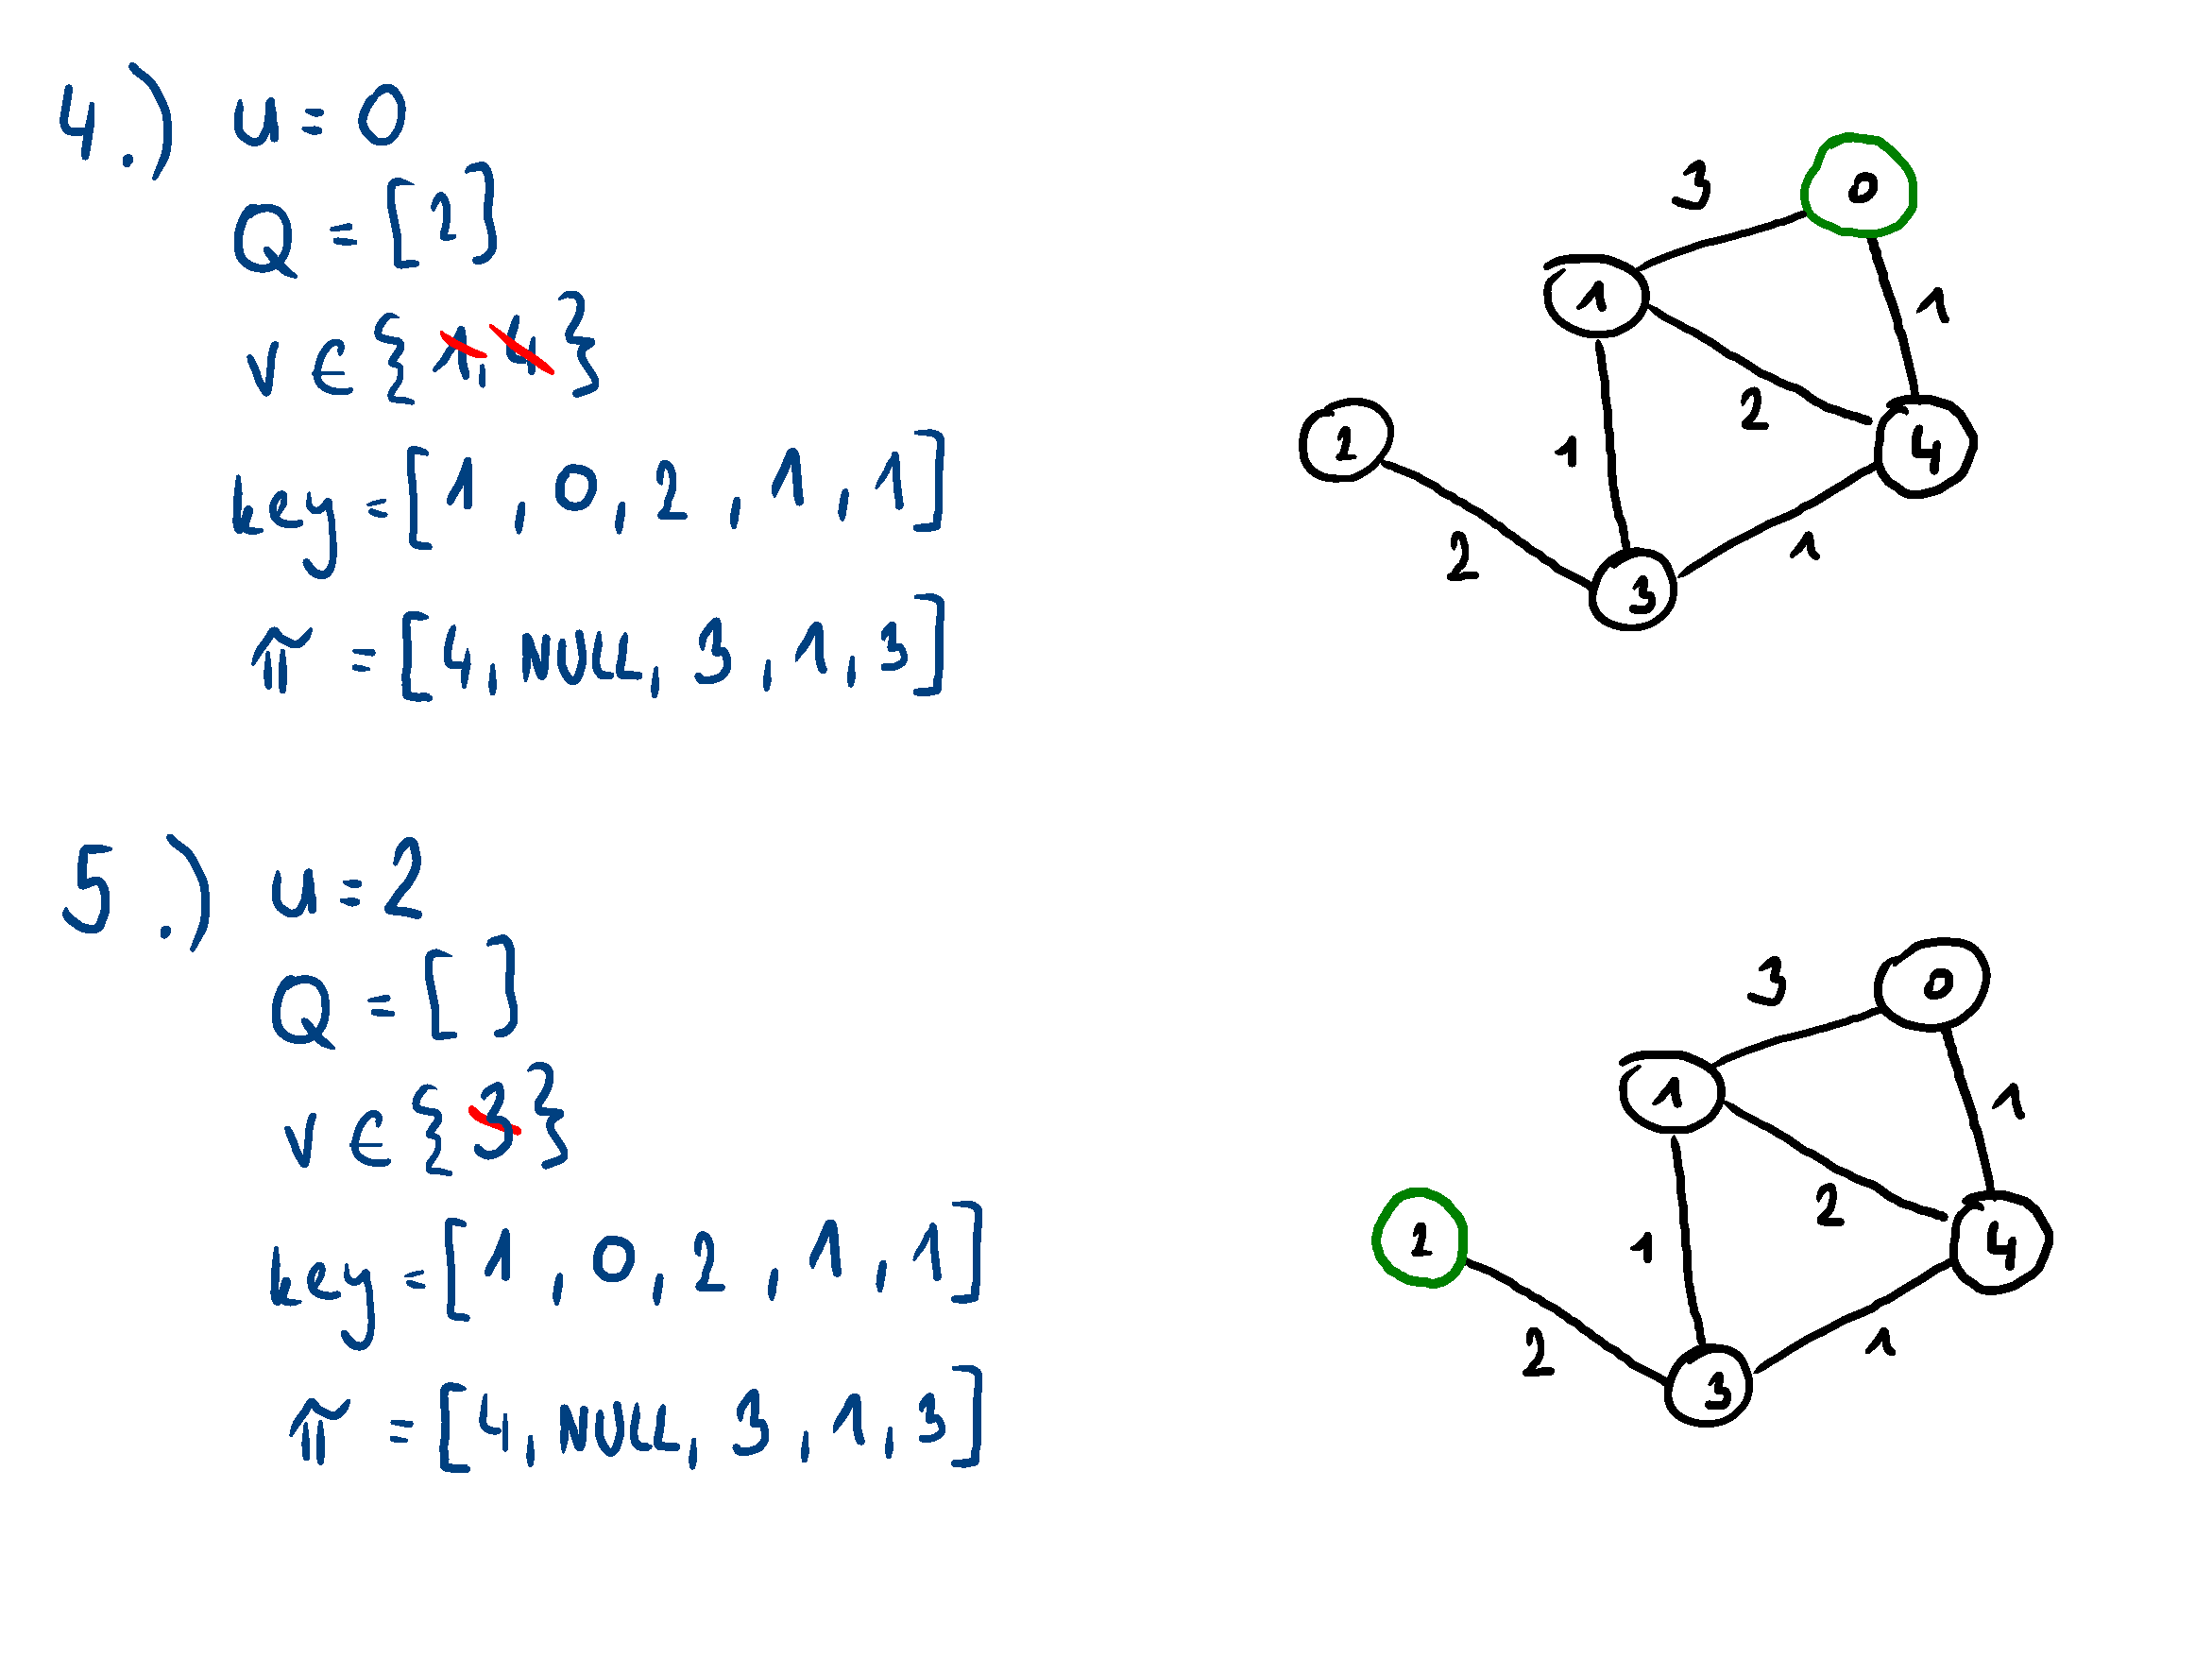
\includegraphics[width=0.9\linewidth]{03-minimalni-kostry-18.pdf}
    \caption{Příklad, část 3.}
\end{figure}

\begin{figure}[H]
    \centering
    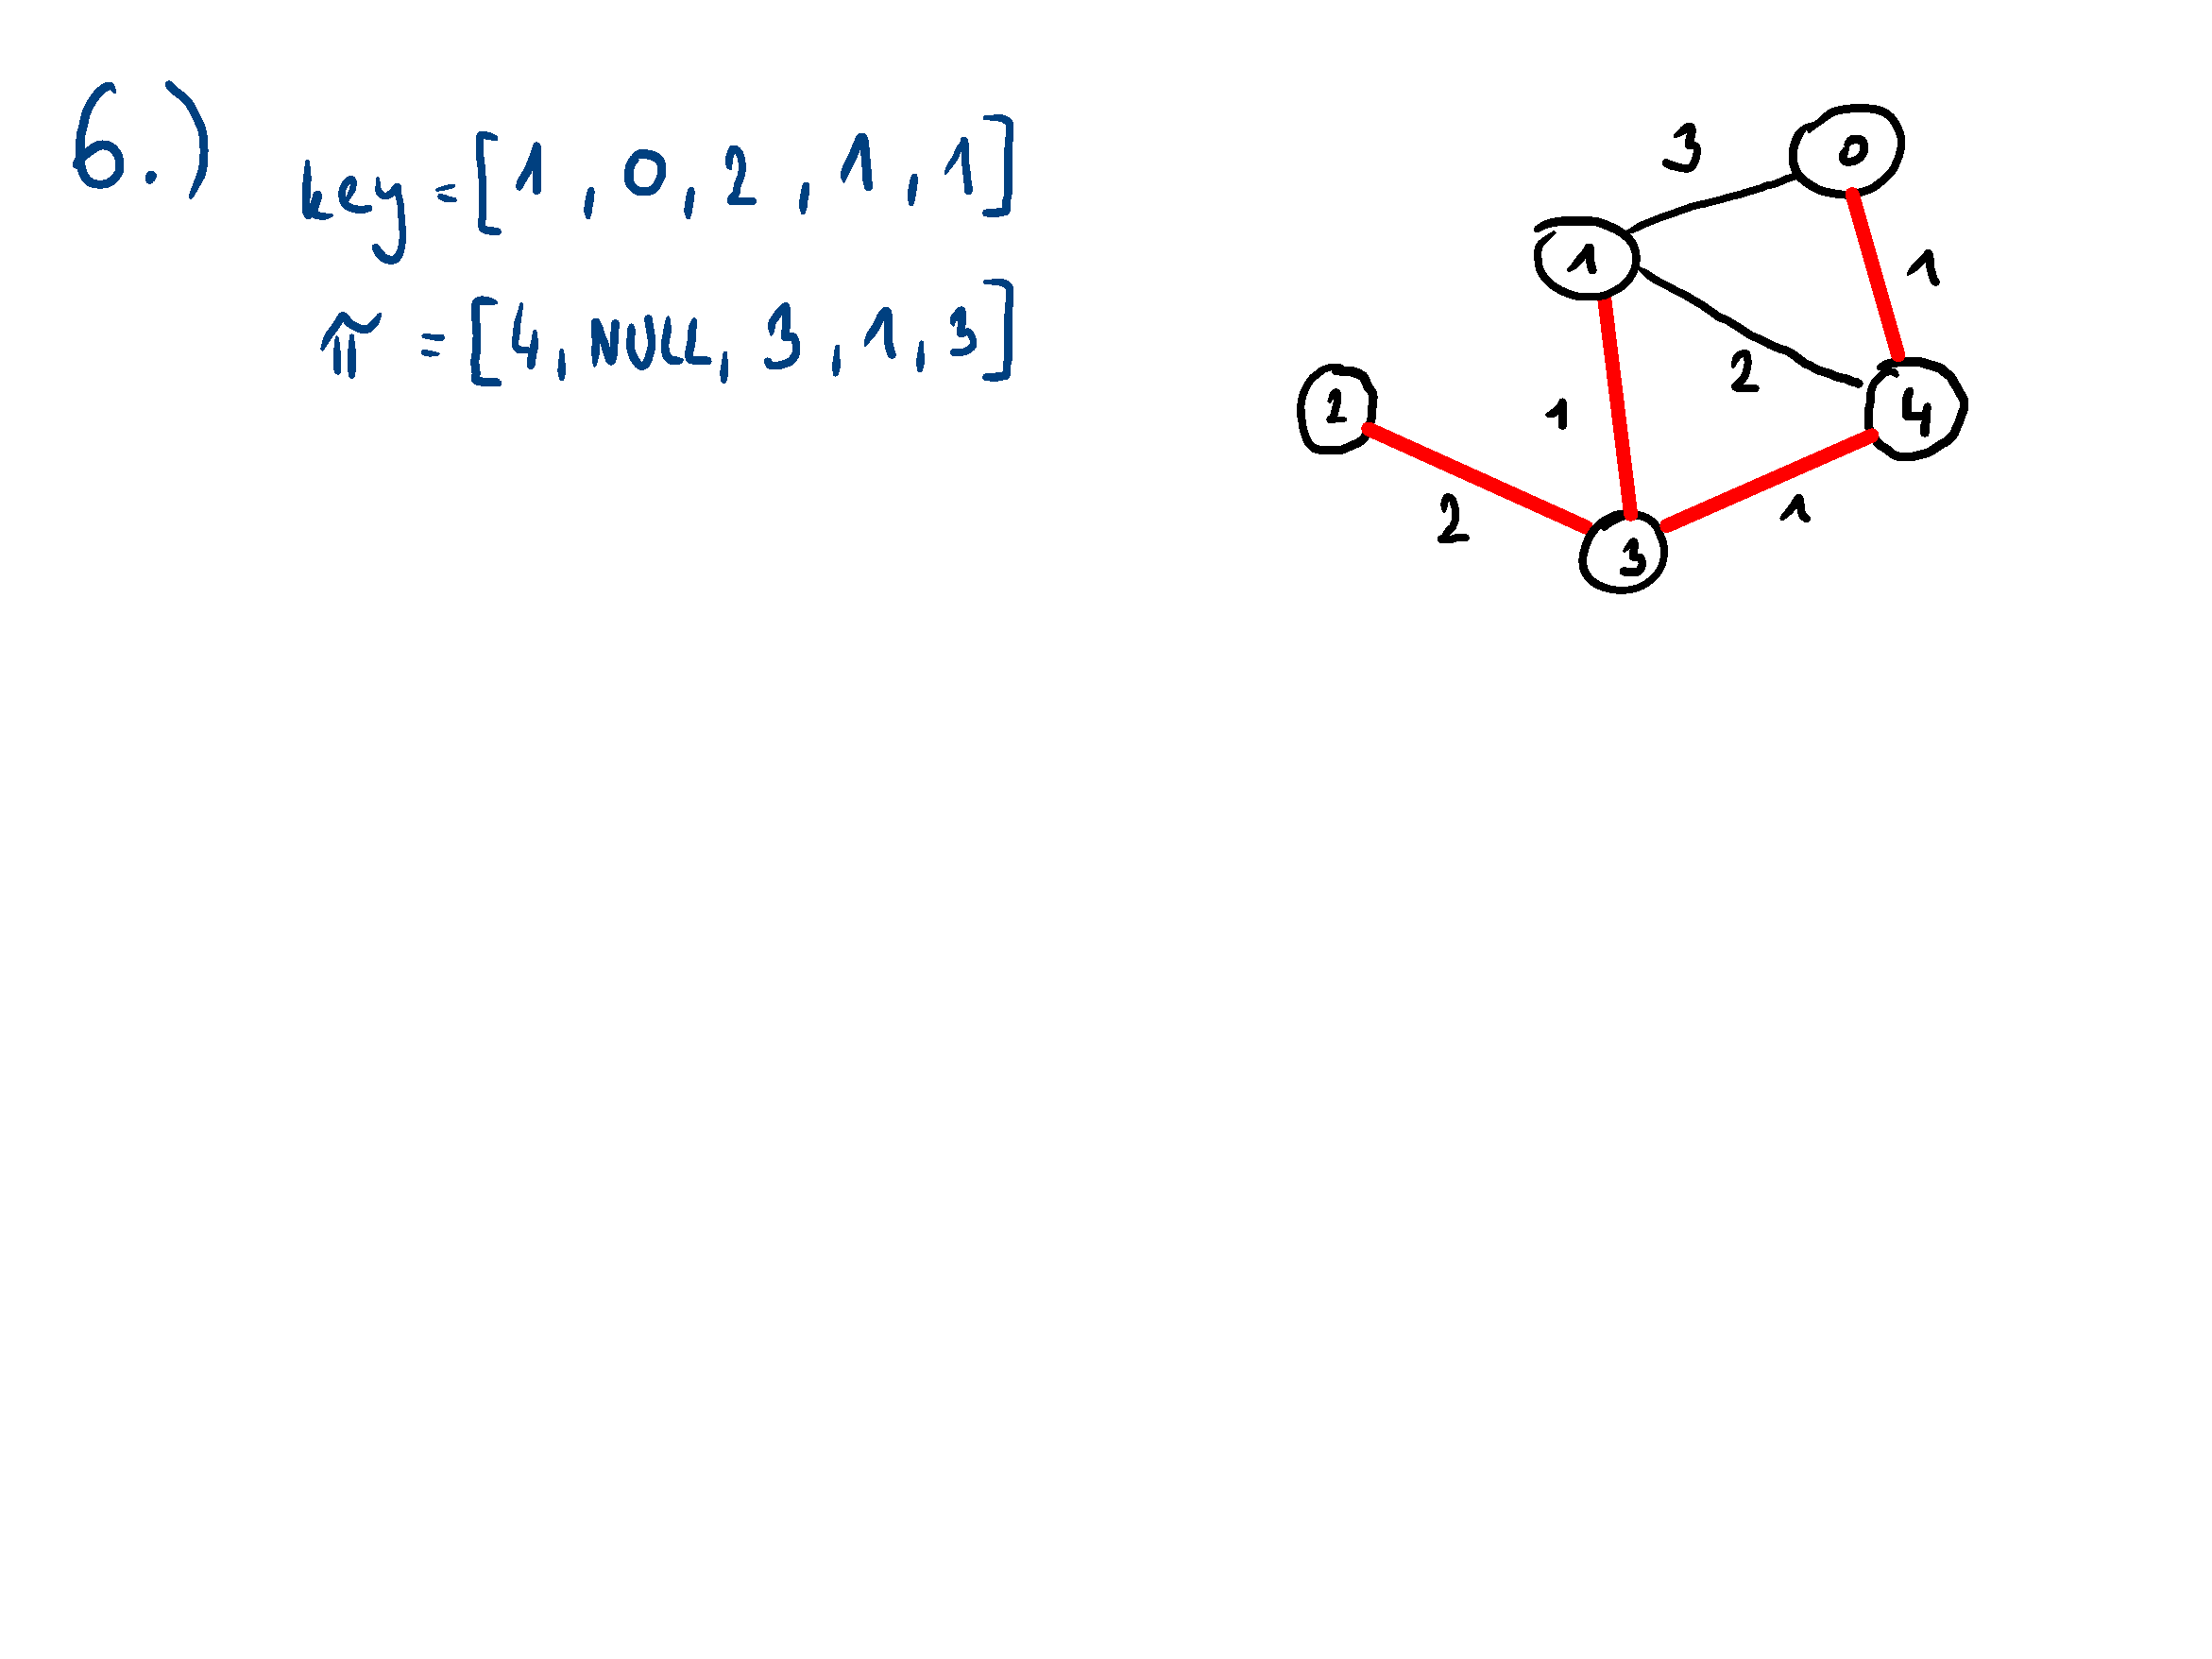
\includegraphics[width=0.9\linewidth]{03-minimalni-kostry-19.pdf}
    \caption{Příklad, část 4.}
\end{figure}

\newpage

% 46
% VUT FIT MITAI
% MSZ 2021/2022
% Author: Vladimir Dusek
% Login: xdusek27

%%%%%%%%%%%%%%%%%%%%%%%%%%%%%%%%%%%%%%%%%%%%%%%%%%%%%%%%%%%%%%%%%%%%%%%%%%%%%%%%

% Path to figures
\graphicspath{{gal/hledani_nejkratsich_cest/figures}}

%%%%%%%%%%%%%%%%%%%%%%%%%%%%%%%%%%%%%%%%%%%%%%%%%%%%%%%%%%%%%%%%%%%%%%%%%%%%%%%%

\chapter{GAL -- Hledání nejkratších cest ze zdrojového uzlu do všech ostatních uzlů grafu (Bellman-Fordův algoritmus, Dijkstrův algoritmus).}

%%%%%%%%%%%%%%%%%%%%%%%%%%%%%%%%%%%%%%%%%%%%%%%%%%%%%%%%%%%%%%%%%%%%%%%%%%%%%%%%

\section{Zdroje}

\begin{compactitem}
    \item \path{gal-handouts.pdf}
    \item \path{GAL_2020-11-05.mp4}
\end{compactitem}

%%%%%%%%%%%%%%%%%%%%%%%%%%%%%%%%%%%%%%%%%%%%%%%%%%%%%%%%%%%%%%%%%%%%%%%%%%%%%%%%

\section{Úvod a kontext}

\paragraph*{Cena cesty} Nechť $G = (V, E)$ je ohodnocený graf s váhovou funkcí $w: E \mapsto \mathbb{R}$. Cena cesty $p = \langle v_o, v_1, \dots, v_k \rangle$ je suma $$
w(p) = \sum_{i=0}^k w(v_i, v_{i+1})
$$.

\paragraph*{Cena nejkratší cesty} Cena nejkratší cesty z $u$ do $v$ je $$
\delta(u, v) = \begin{cases}
    min( \{ w(p) : u \xRightarrow{\text{p}} v \} ) \\
    \infty   \text{pokud cesta neexistuje}
\end{cases}
$$.

\paragraph*{Nejkratší cesta} Nejkratší cesta z $u$ do $v$ je pak libovolná cesta $p$ taková, že $w(p) = \delta(u, v)$.

\paragraph*{Cena cesty se záporným cyklem} Pokud na cestě z $u$ do $v$ existuje záporný cyklus (cyklus jehož celková cena je záporná), pak $\delta(u, v) = - \infty$.

\paragraph*{Záporné ohodnocení hran} Pokud na cestě z $u$ do $v$ neexistuje záporný cyklus, tak algoritmy pracují dobře i se záporným ohodnocením hran.

\paragraph*{Reprezentace cesty} Cestu reprezentujeme pomocí pole předchůdců $\pi$.

\paragraph*{Hledání nejkratších cest ze všech uzlů do jednoho} Tento problém lze řešit stejnými algoritmy. Graf se transponuje (převrácení orientace hran), provede se algoritmus pro problém \uv{hledání nejkratších cest ze jednoho uzlu do všech ostatních uzlů} a poté se transponuje zpět.

\paragraph*{Reprezentace nejkratší cesty} Nejkratší cestu grafu $G = (V, E)$ reprezentujeme pomocí pole předchůdců $\pi$, kde $\pi[v]$ označuje předchůdce uzlu $v \in V$ na nejkratší cestě. Podgraf předchůdců pak je $G_{\pi} = (V_{\pi}, E_{\pi})$, $V_{\pi} = \{ v \in V : \pi[v] \neq \text{NULL} \} \cup \{ s \}$, $E_{\pi} = \{ (\pi[v], v) \in E : v \in V_{\pi} - \{ s \}$. V okamžiku dokončení algoritmu výpočtu nejkratších cest je $G_{\pi}$ strom nejkratších cest. Tj. kořenový strom obsahující nejkratší cesty ze zdroje $s$ do všech ostatních uzlů.

%%%%%%%%%%%%%%%%%%%%%%%%%%%%%%%%%%%%%%%%%%%%%%%%%%%%%%%%%%%%%%%%%%%%%%%%%%%%%%%%

\section{Pomocné funkce}

Představené algoritmy pracují z důvodu efektivity se sledy a nikoliv s cestami (bylo by nutné stále kontrolovat, zda nebyla porušena podmínka cesty), ačkoliv je problém nazývá hledání nejkratší cesty.

\bigskip\noindent\begin{minipage}{\linewidth}
\begin{lstlisting}[language=Python, caption={Pomocná inicializační funkce. Složitost je $\Theta(n)$, kde $n$ je počet uzlů.}]
def initialize_single_source(G, s):
    # G je graf
    # s je vychozi uzel
    for v in G.V:
        d[v] = INF  # d je pole vzdalenosti
        pi[v] = NULL  # pi je pole predchudcu
    d[s] = 0
\end{lstlisting}
\end{minipage}

\noindent\begin{minipage}{\linewidth}
\begin{lstlisting}[language=Python, caption={Pomocná funkce \textit{relax}. Složitost je $O(1)$.}]
def relax(u, v, w):
    # u a v jsou uzly grafu
    # w je vahova funkce
    if d[v] > d[u] + w(u, v):
        d[v] = d[u] + w(u, v)
        pi[v] = u
\end{lstlisting}
\end{minipage}

\begin{figure}[H]
    \centering
    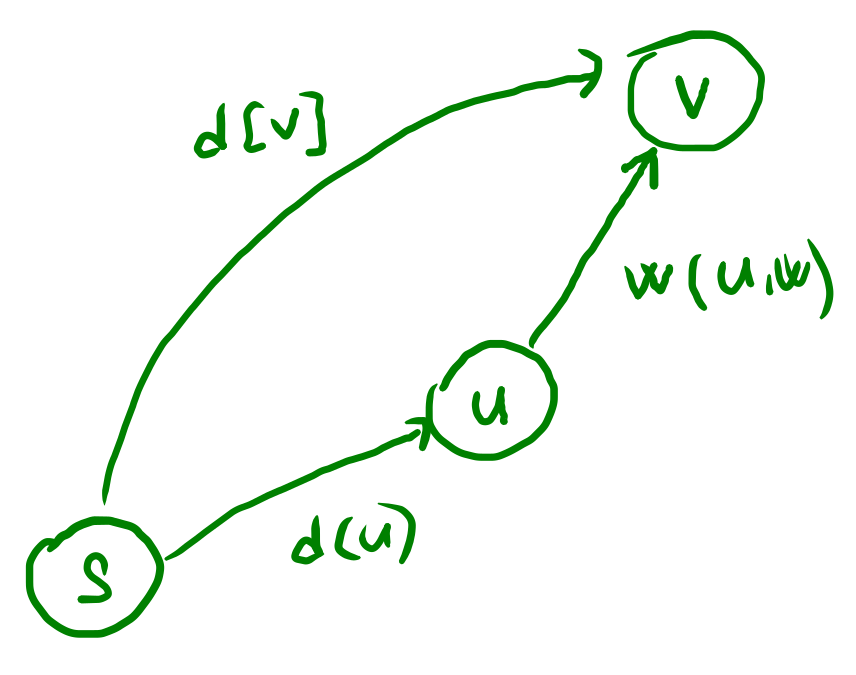
\includegraphics[width=0.4\linewidth]{relax.png}
    \caption{Ukázka činnosti funkce \textit{relax}.}
\end{figure}

%%%%%%%%%%%%%%%%%%%%%%%%%%%%%%%%%%%%%%%%%%%%%%%%%%%%%%%%%%%%%%%%%%%%%%%%%%%%%%%%

\section{Bellman-Fordův algoritmus}

Slouží pro řešení v obecných grafech, mohou obsahovat cykly a záporné hrany. Záporné cykly je však nutné detekovat a vrátit specifickou hodnotu. V podstatě se jedná o \textit{brute force} algoritmus, provede se relaxace $n-1$-krát pro každou hranu.

\bigskip\noindent\begin{minipage}{\linewidth}
\begin{lstlisting}[language=Python, caption={Algoritmus Bellman-Ford. Proč $n-1$ iterací? Protože mezi libovolnými dvěma uzly v grafu, existuje cesta o maximálním počtu hran $n-1$.}]
def bellman_ford(G, s, w):
    # G je graf
    # s je vychozi uzel
    # w je vahova funkce

    # faze inicializace
    initialize_single_source(G, s)
    n = len(G.V) # pocet uzlu

    # faze relaxace: provedeni (n-1) * m relaxaci (m je pocet hran)
    for _ in range(0, n-1):
        for u, v in G.E:
            relax(u, v, w)

    # faze detekce zaporneho cyklu
    for u, v in G.E:
        if d[u] > d[v] + w(u, v):
            return NULL

    return pi
\end{lstlisting}
\end{minipage}

\subsection{Složitost}

\begin{compactitem}
    \item Řádek 7, 8 -- $\Theta(1)$.
    \item Řádky 11, 12, 13 -- $(n-1) \cdot \Theta(m) = \Theta(n \cdot m)$, kde $n$ je počet uzlů a $m$ je počet hran grafu.
    \item Řádek 16, 17, 18 -- $\Theta(m)$.
    \item Celkem $\Theta(n \cdot m)$.
\end{compactitem}

\subsection{Příklad}

\begin{figure}[H]
    \centering
    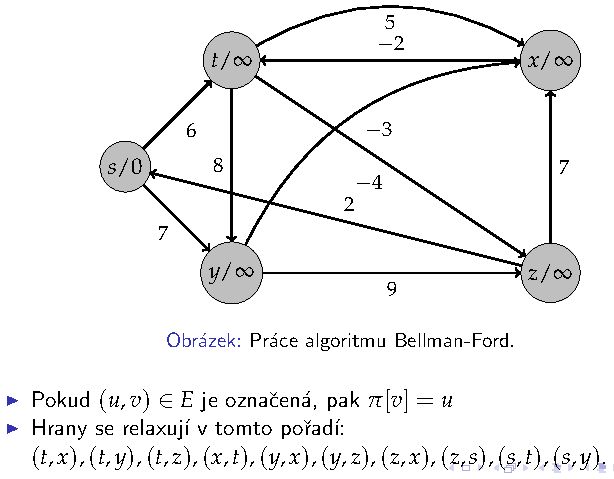
\includegraphics[width=0.75\linewidth]{example_bellman_ford_p1.pdf}
    \caption{Příklad, část 1.}
\end{figure}

\begin{figure}[H]
    \centering
    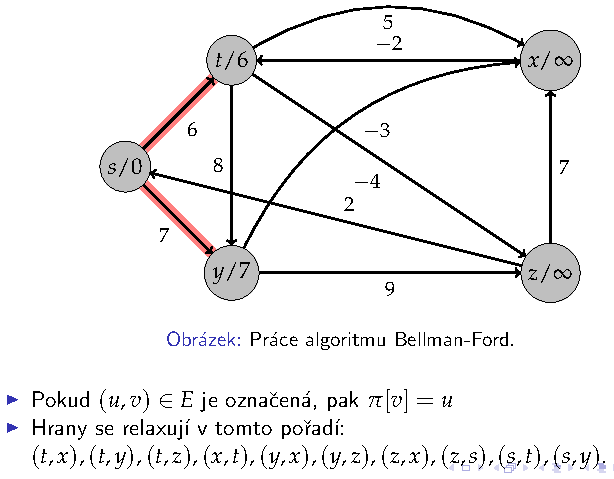
\includegraphics[width=0.75\linewidth]{example_bellman_ford_p2.pdf}
    \caption{Příklad, část 2.}
\end{figure}

\begin{figure}[H]
    \centering
    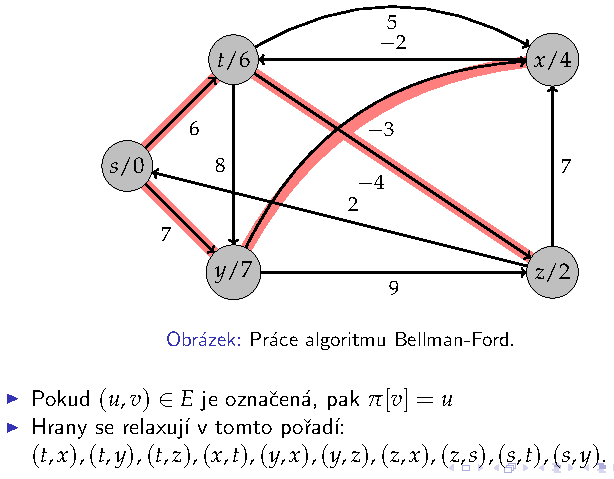
\includegraphics[width=0.75\linewidth]{example_bellman_ford_p3.pdf}
    \caption{Příklad, část 3.}
\end{figure}

\begin{figure}[H]
    \centering
    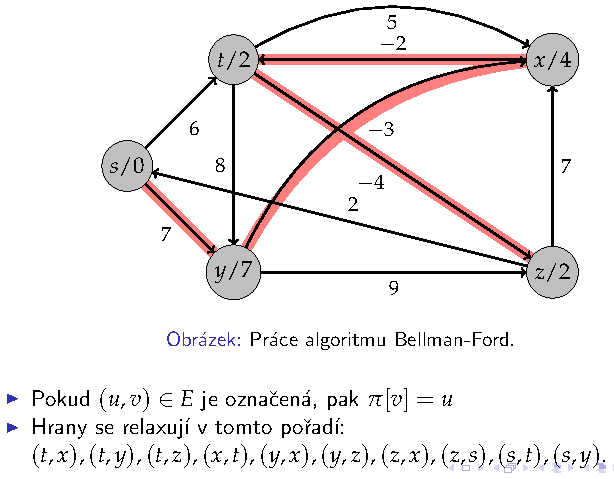
\includegraphics[width=0.75\linewidth]{example_bellman_ford_p4.pdf}
    \caption{Příklad, část 4.}
\end{figure}

\begin{figure}[H]
    \centering
    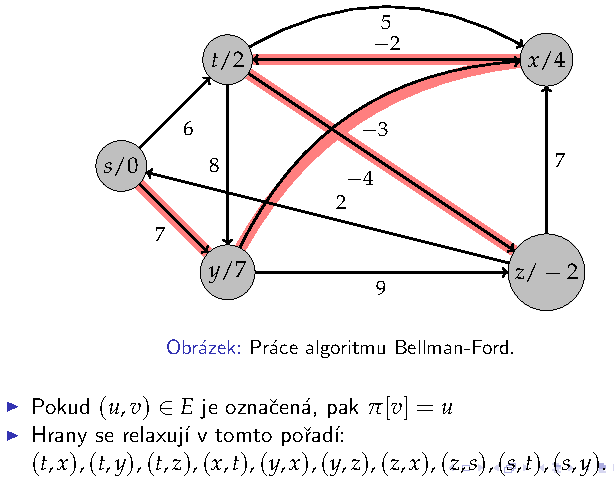
\includegraphics[width=0.75\linewidth]{example_bellman_ford_p5.pdf}
    \caption{Příklad, část 5.}
\end{figure}

%%%%%%%%%%%%%%%%%%%%%%%%%%%%%%%%%%%%%%%%%%%%%%%%%%%%%%%%%%%%%%%%%%%%%%%%%%%%%%%%

\section{Dijkstrův algoritmus}

Slouží pro řešení v acyklických grafech bez záporných hran. Pro takto omezený problém existují rychlejší algoritmy než pro problém v obecných grafech.

\bigskip\noindent\begin{minipage}{\linewidth}
\begin{lstlisting}[language=Python, caption={Algoritmus Dijkstra.}]
def dijkstra(G, s, w):
    # G je graf
    # s je vychozi uzel
    # w je vahova funkce

    # faze inicializace
    initialize_single_source(G, s)
    Q = Queue(G.V) # prioritni fronta uzlu
    S = {} # mnozina uzlu, ktera uz byla prozkoumana

    # faze relaxace
    while not Q.empty():
        u = Q.extract_min(d) # vrati prvek z Q s nejmensi hodnotou v d
        S += {u}
        # pro vsechny sousedy uzlu u (Adj je seznam sousedu)
        for v in Adj[u]:
            relax(u, v, w)

        Q.decrease_key(d) # aktualizace prioritni fronty

    return d, pi
\end{lstlisting}
\end{minipage}

\subsection{Složitost}

\begin{compactitem}
    \item Předpokládejme implementaci prioritní fronty pomocí pole.
    \item Řádek 8, 18 -- $O(1)$.
    \item Řádek 11 -- While cyklus se provede $n$-krát, kde $n$ je počet uzlů.
    \item Řádek 12 -- $O(n)$, najítí minima v poli uzlů. Celkově (s cyklem) $O(n^2)$.
    \item Řádek 16 -- $O(m)$, pro všechny hrany. Celkově (s cyklem) $O(m \cdot n)$.
    \item Celkem $O(n^2 + m) = O(n^2)$.
    \item Pro řídké grafy lze využít implementaci fronty pomocí binární haldy a získat tak $O(m \cdot \log(n))$.
    \item Při implementaci fronty pomocí Fibonacciho haldy dostaneme časovou složitost $O(n \cdot \log(n) + m)$.
\end{compactitem}

\subsection{Příklad}

\begin{figure}[H]
    \centering
    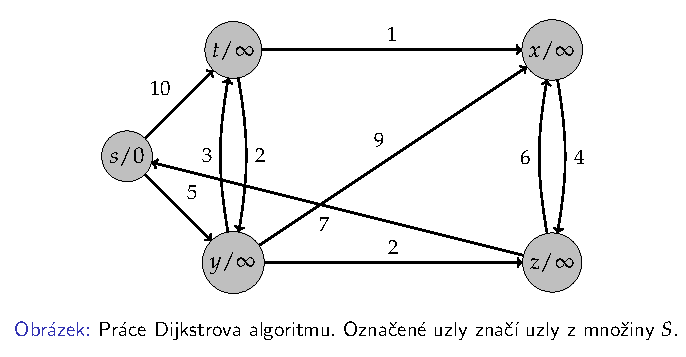
\includegraphics[width=0.80\linewidth]{example_dijkstra_p1.pdf}
    \caption{Příklad, část 1.}
\end{figure}

\begin{figure}[H]
    \centering
    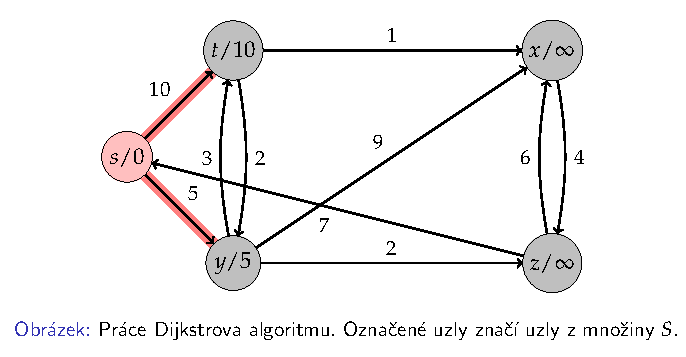
\includegraphics[width=0.80\linewidth]{example_dijkstra_p2.pdf}
    \caption{Příklad, část 2.}
\end{figure}

\begin{figure}[H]
    \centering
    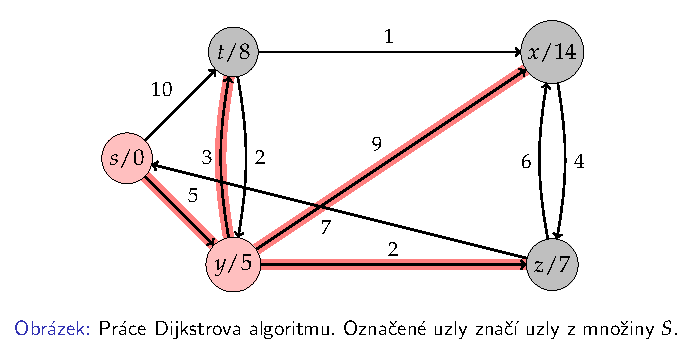
\includegraphics[width=0.80\linewidth]{example_dijkstra_p3.pdf}
    \caption{Příklad, část 3.}
\end{figure}

\begin{figure}[H]
    \centering
    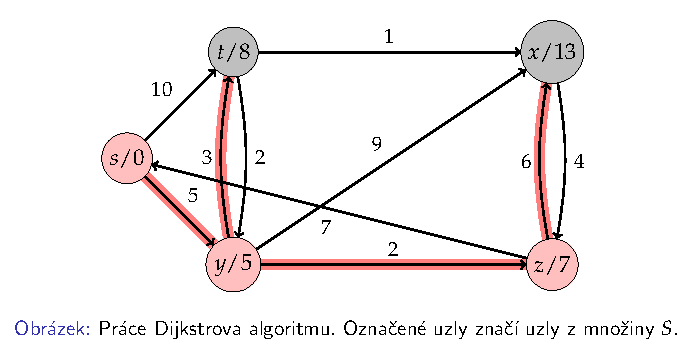
\includegraphics[width=0.80\linewidth]{example_dijkstra_p4.pdf}
    \caption{Příklad, část 4.}
\end{figure}

\begin{figure}[H]
    \centering
    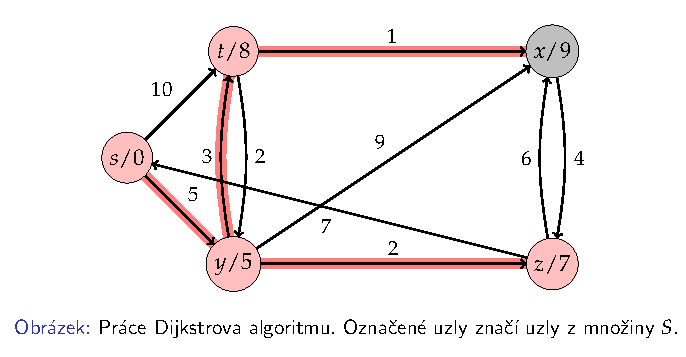
\includegraphics[width=0.80\linewidth]{example_dijkstra_p5.pdf}
    \caption{Příklad, část 5.}
\end{figure}

\begin{figure}[H]
    \centering
    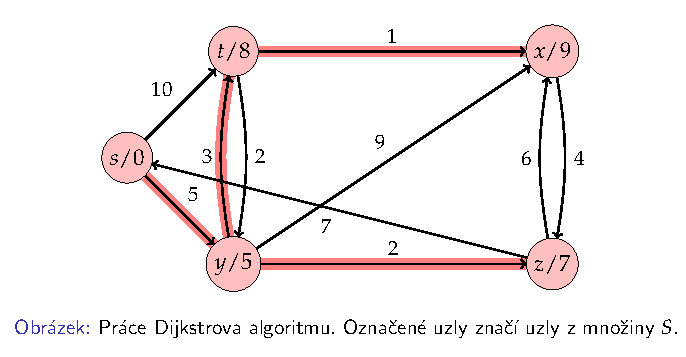
\includegraphics[width=0.80\linewidth]{example_dijkstra_p6.pdf}
    \caption{Příklad, část 6.}
\end{figure}

\newpage

% 47
% VUT FIT MITAI
% MSZ 2021/2022
% Author: Vladimir Dusek
% Login: xdusek27

%%%%%%%%%%%%%%%%%%%%%%%%%%%%%%%%%%%%%%%%%%%%%%%%%%%%%%%%%%%%%%%%%%%%%%%%%%%%%%%%

% Path to figures
\graphicspath{{pdi/volba_koordinatora/figures}}

%%%%%%%%%%%%%%%%%%%%%%%%%%%%%%%%%%%%%%%%%%%%%%%%%%%%%%%%%%%%%%%%%%%%%%%%%%%%%%%%

\chapter{PDI -- Klasifikace algoritmů volby koordinátora, algoritmus Bully a jeho složitost.}
\label{chapter_pdi_koordinator}

%%%%%%%%%%%%%%%%%%%%%%%%%%%%%%%%%%%%%%%%%%%%%%%%%%%%%%%%%%%%%%%%%%%%%%%%%%%%%%%%

\section{Zdroje}

\begin{compactitem}
    \item \path{07_Synchronization.pdf}
    \item \path{PDI_2020-11-02.mp4}
\end{compactitem}

%%%%%%%%%%%%%%%%%%%%%%%%%%%%%%%%%%%%%%%%%%%%%%%%%%%%%%%%%%%%%%%%%%%%%%%%%%%%%%%%

\section{Úvod a kontext}

\begin{compactitem}
    \item Mějme množinu procesů v~rámci distribuovaného systému. Řešíme problém nalezení shody na nějaké věci (synchronizační problém). Problém můžeme rozdělit na dvě situace: \begin{compactitem}
        \item \textbf{Problém volby koordinátora} -- Výběr jednoho z~procesů, který bude vedoucím procesem (koordinátor). Tento proces pak může vykonat určitou činnost nebo může sloužit ostatním procesům k~realizaci význačné role v~systému.

        \item \textbf{Problém vzájemného vyloučení} -- Předpokládejme, že konkrétní zdroj může v~daném okamžiku používat pouze jeden proces. Tento problém se běžně vyskytuje ve víceprocesorových systémech, ale také v~distribuovaných systémech.
    \end{compactitem}

    \item Synchronizační problémy lze v~rámci operačních systémů nebo multiprocesorových systémů řešit pomocí provádění atomických operací, sdílené paměti apod. -- je pro ně podpora v~rámci operačního systému nebo hardwaru. V~distribuovaných systémech takovéto prostředky nejsou často k dispozici, proto se synchronizační problémy řeší pomocí zasílání zprav, resp. algoritmicky.
\end{compactitem}

%%%%%%%%%%%%%%%%%%%%%%%%%%%%%%%%%%%%%%%%%%%%%%%%%%%%%%%%%%%%%%%%%%%%%%%%%%%%%%%%

\section{Problém volby koordinátora}

\begin{compactitem}
    \item Předpokládáme:
    \begin{compactitem}
        \item Každý proces má unikátní ID.
        \item Procesy neznají stav (běžící, neběžící) dalších procesů.
        \item Každý proces zná ID dalších procesů (záleží na topologii).
    \end{compactitem}
    \item Cíl:
    \begin{compactitem}
        \item Dosáhnutí shody mezi všemi procesy na procesu, který je koordinátor.
        \item Kritérium výběru koordinátora může být různé. Např. na základě proces ID (proces s~největším ID se stane koordinátorem).
    \end{compactitem}
\end{compactitem}

%%%%%%%%%%%%%%%%%%%%%%%%%%%%%%%%%%%%%%%%%%%%%%%%%%%%%%%%%%%%%%%%%%%%%%%%%%%%%%%%

\section{Bully algoritmus}

\begin{compactitem}
    \item Pro topologii každý s~každým -- každý proces může komunikovat s~každým dalším procesem.

    \item Používá tři druhy zpráv: ELECTION, OK, COORDINATOR.
\end{compactitem}

\subsection{Postup}

\begin{compactitem}
    \item Proces P, který má podezření, že chybí koordinátor, může zahájit volby.
    \begin{compactenum}
        \item Proces P odešle zprávu ELECTION všem procesům s~větším ID.
        \item Pokud nikdo neodpoví, P vyhrává volby a stává se koordinátorem.
        \item Pokud některý z~procesů s~větším ID odpoví (zpráva OK), tak přebírá řízení a práce P je ukončena.
        \item Pokud P obdrží zprávu ELECTION od procesů s~menším ID, pošle jim odpověď OK na zablokování procesů.
    \end{compactenum}
    \item Nakonec zůstane pouze P (nový koordinátor), který o~tom informuje ostatní zasláním zprávy COORDINATOR.
    \item Pokud se proces probudí nebo je restartován, první akcí je vyvolání voleb.
\end{compactitem}

\subsection{Složitost}

\begin{compactitem}
    \item Složitost z~hlediska počtu zpráv.

    \item Nejhorší případ (iniciátor s~nejmenším ID): \begin{compactitem}
        \item $(n-1)$ iterací
        \item $2(n-1)$ zpráv ELECTION a OK pro každou iteraci
        \item $(n-1)$ zpráv COORDINATOR
        \item Celkem: $(n-1) \times 2(n-1) + (n-1) \approx n^2$
    \end{compactitem}

    \item Nejlepší případ (iniciátor s~největším ID): \begin{compactitem}
        \item $(n-1)$ zpráv COORDINATOR
        \item Celkem: $(n-1)$
    \end{compactitem}
\end{compactitem}

\subsection{Příklad}

\begin{figure}[H]
    \centering
    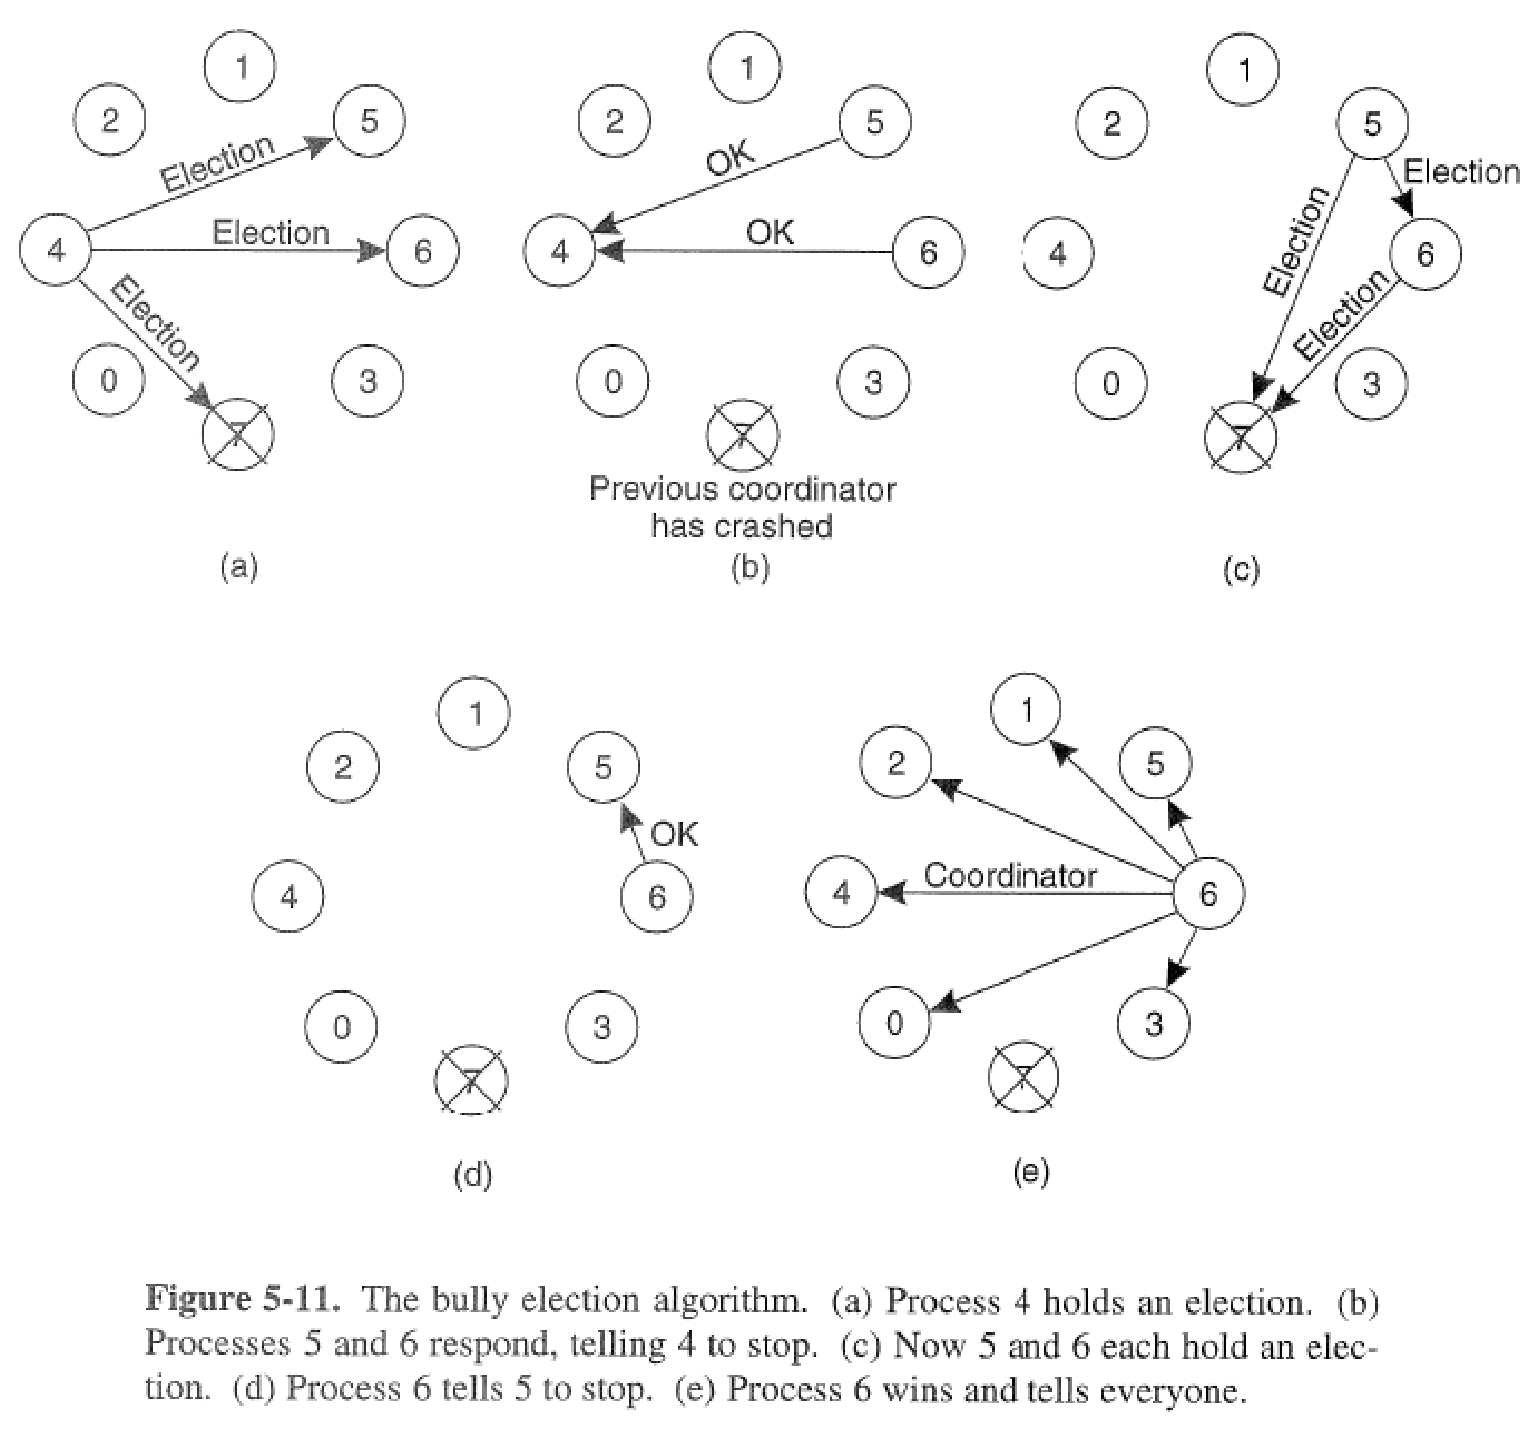
\includegraphics[width=1\linewidth]{example_bully.pdf}
    \caption{Příklad činnosti Bully algoritmu.}
\end{figure}

%%%%%%%%%%%%%%%%%%%%%%%%%%%%%%%%%%%%%%%%%%%%%%%%%%%%%%%%%%%%%%%%%%%%%%%%%%%%%%%%

\section{Ring Algoritmus}

\begin{compactitem}
    \item Pro kruhovou topologii -- procesy jsou uspořádané do kruhu podle svého proces ID.

    \item Každý proces musí vědět nejenom o~svém následovníkovi, ale také o~jeho následníkovi, který funguje jako \uv{záloha}, v~případě že by se přímý následník stal nedostupný.

    \item Používá dva druhy zpráv: ELECTION, COORDINATOR.
\end{compactitem}

\subsection{Postup}

\begin{compactitem}
    \item Proces P, který má podezření, že chybí koordinátor, může zahájit volby.
    \begin{compactenum}
        \item Zašle zprávu ELECTION obsahující jeho ID dalšímu procesu (pokud další proces nereaguje, proces P zašle stejnou zprávu dalšímu v~kruhu).
        \item Každý člen topologie přijme zprávu ELECTION, přidá do ní své ID a přepošle zprávu dalšímu procesu.
    \end{compactenum}
    \item Když se zpráva vrátí k~procesu P, je zpráva převedena na zprávu  COORDINATOR a poslána následujícímu procesu v~topologii, aby bylo možné nahlásit:
    \begin{compactenum}
        \item Novým koordinátorem se stává proces s~nejvyšším ID.
        \item Členové sítě jsou stále aktivní.
    \end{compactenum}
    \item Po síti může obíhat více zpráv zároveň.
\end{compactitem}

\subsection{Složitost}

\begin{compactitem}
    \item Složitost z~hlediska počtu zpráv.
    \item Vždy $2n \approx n$ zpráv. Jedno kolečko \uv{oběhne} zpráva ELECTION a druhé zpráva COORDINATOR.
\end{compactitem}

\subsection{Příklad}

\begin{figure}[H]
    \centering
    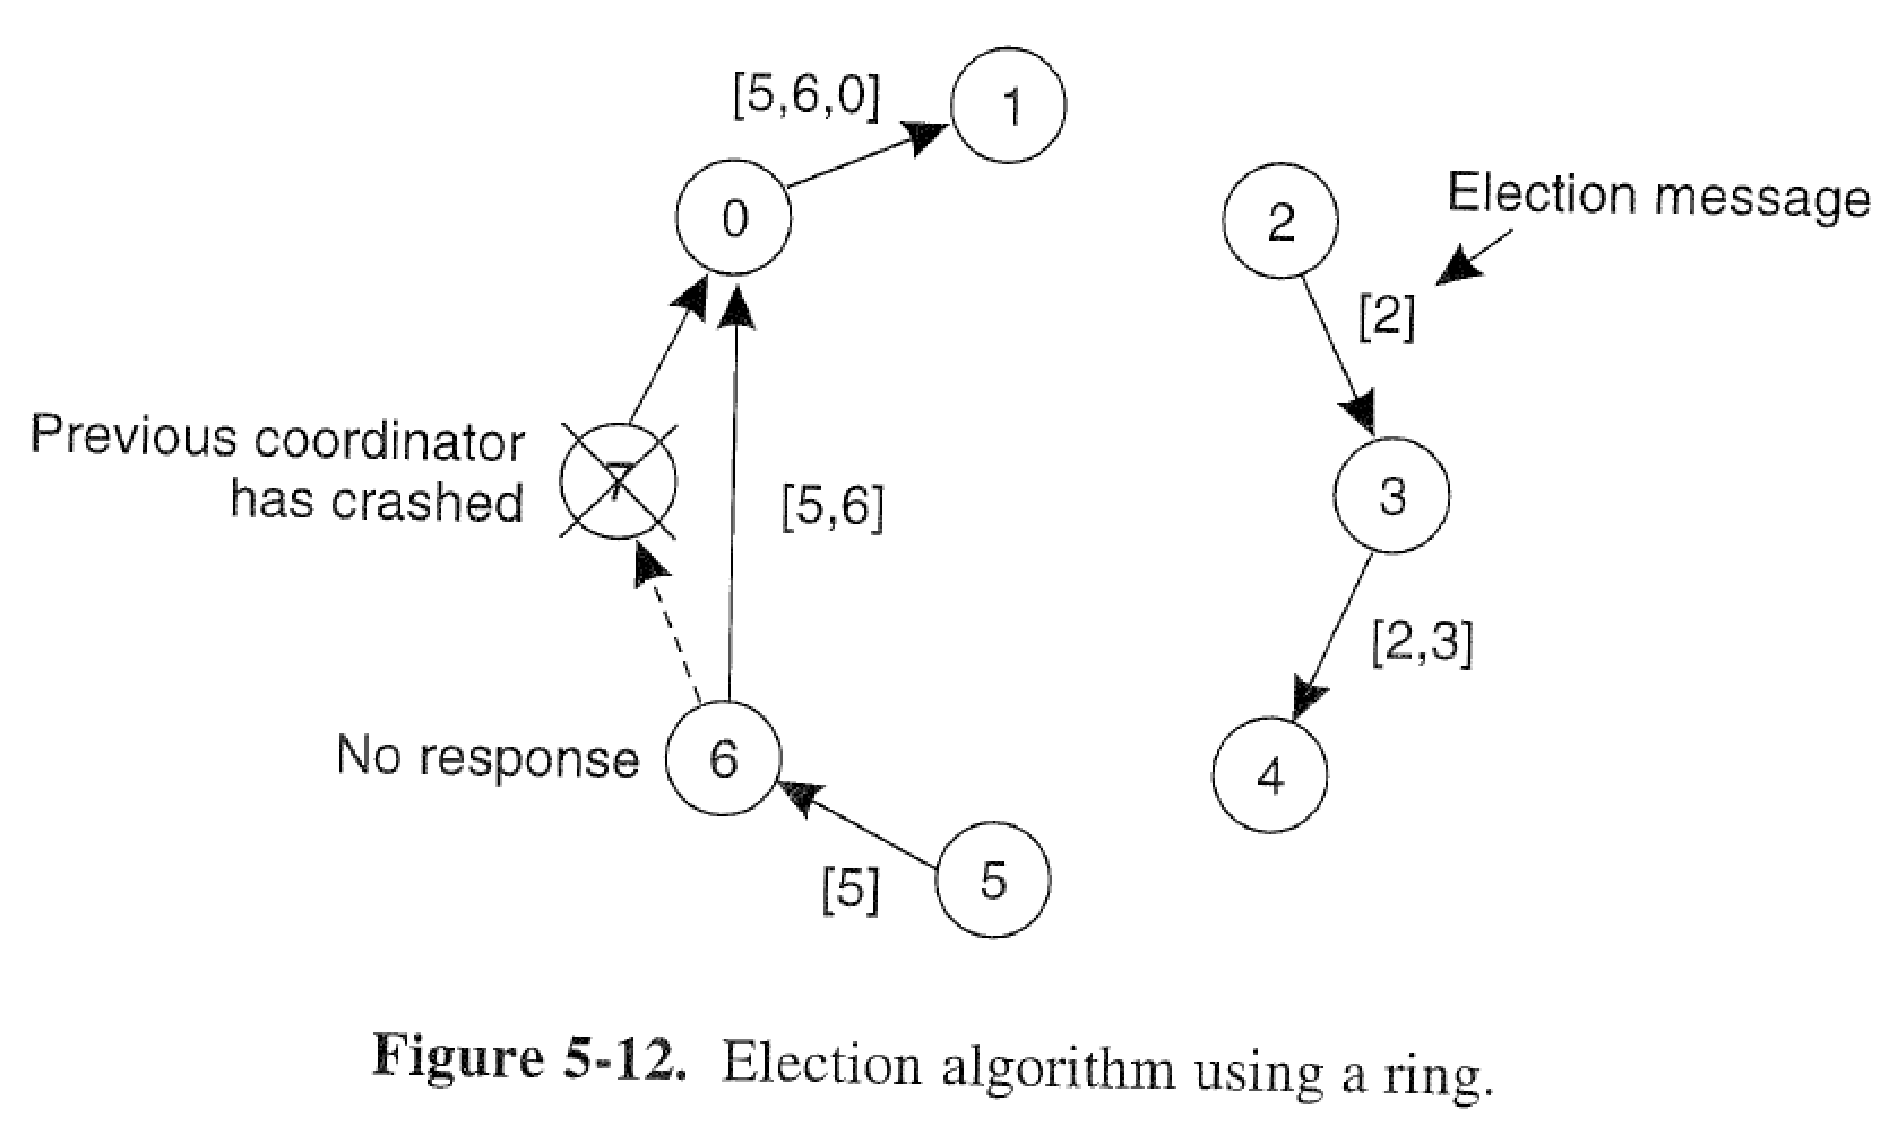
\includegraphics[width=1\linewidth]{example_ring.pdf}
    \caption{Příklad činnosti Ring algoritmu.}
\end{figure}

%%%%%%%%%%%%%%%%%%%%%%%%%%%%%%%%%%%%%%%%%%%%%%%%%%%%%%%%%%%%%%%%%%%%%%%%%%%%%%%%

\section{Algoritmus pro obecnou topologii}

\begin{compactitem}
    \item Předpokládáme, že nemáme ani kruhovou topologii ani spojení každý s~každým. Např.: peer-to-peer sítě, sensorové sítě, \dots
\end{compactitem}

\subsection{Postup}

\begin{compactitem}
    \item V~první iteraci se broadcastem posílá zpráva ELECTION.
    \item Každý uzel si uloží od kterého souseda dostal zprávu ELECTION jako první. Tím vzníká kostra grafu (\textit{spanning tree}).
    \item Uložený soused je poté využijí pro zpětnou komunikaci. To znamená, že další komunikace už probíhá přes strom, nikoliv přes broadcast. Tím je ušetřena některé komunikace.
\end{compactitem}

\subsection{Složitost}

\begin{compactitem}
    \item Složitost z~hlediska počtu zpráv.
    \item Inicializační broadcast: počet hran grafu.
    \item Odpověď: počet hran kostry grafu.
    \item Result broadcast: počet hran kostry grafu.
\end{compactitem}

\subsection{Příklad}

\begin{figure}[H]
    \centering
    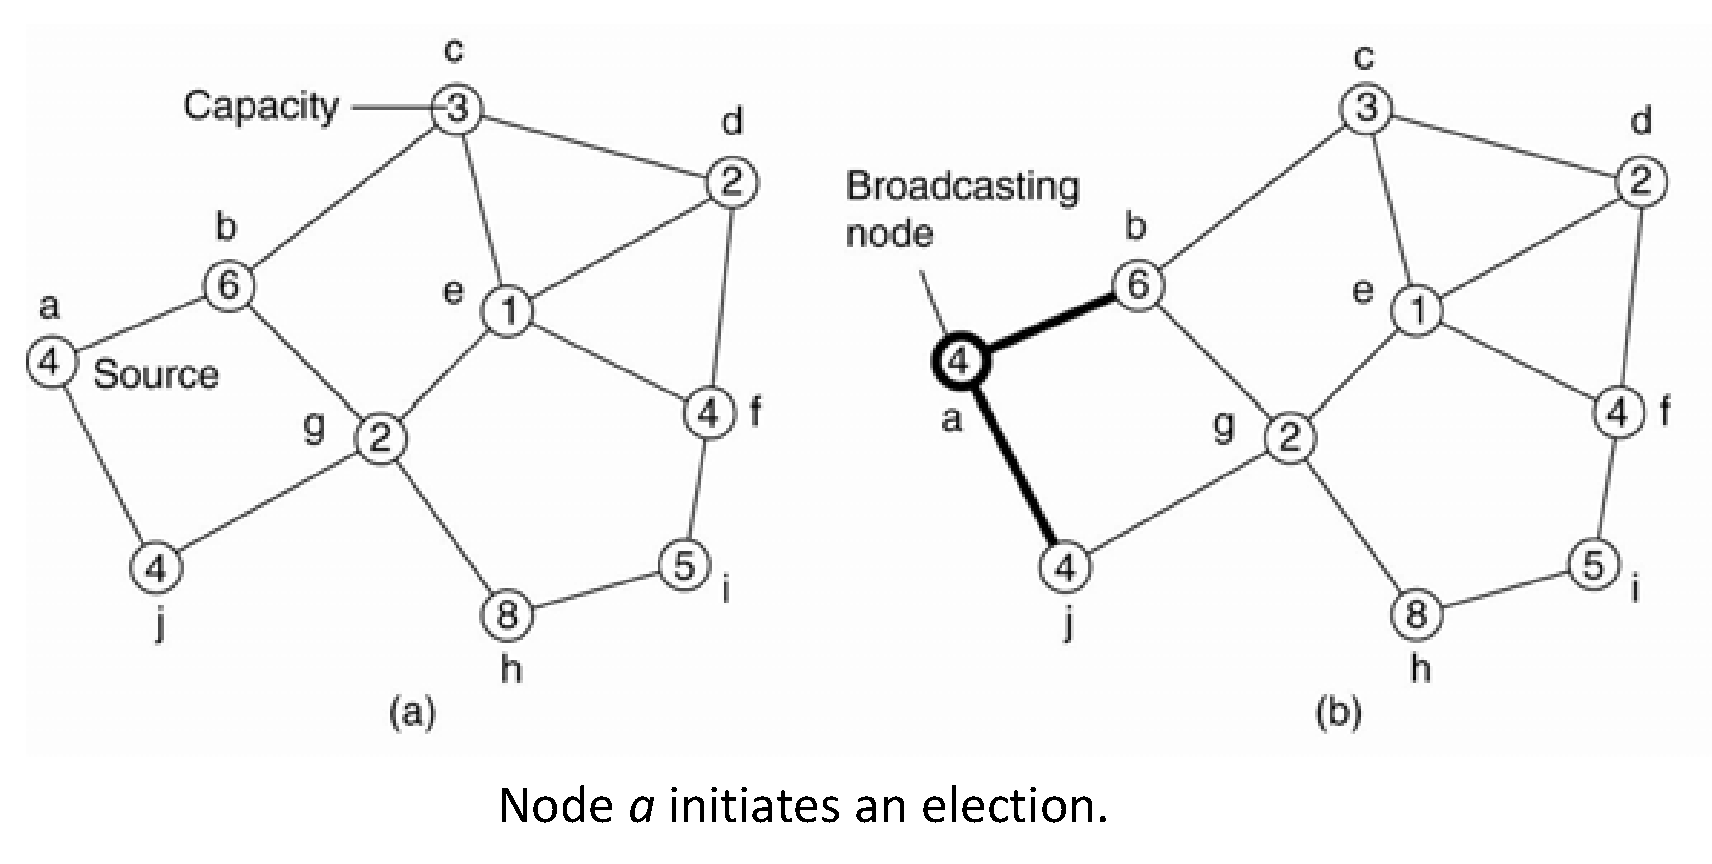
\includegraphics[width=1\linewidth]{example_general_topology_p1.pdf}
    \caption{Příklad činnosti algoritmu pro obecnou topologii, část 1.}
\end{figure}

\begin{figure}[H]
    \centering
    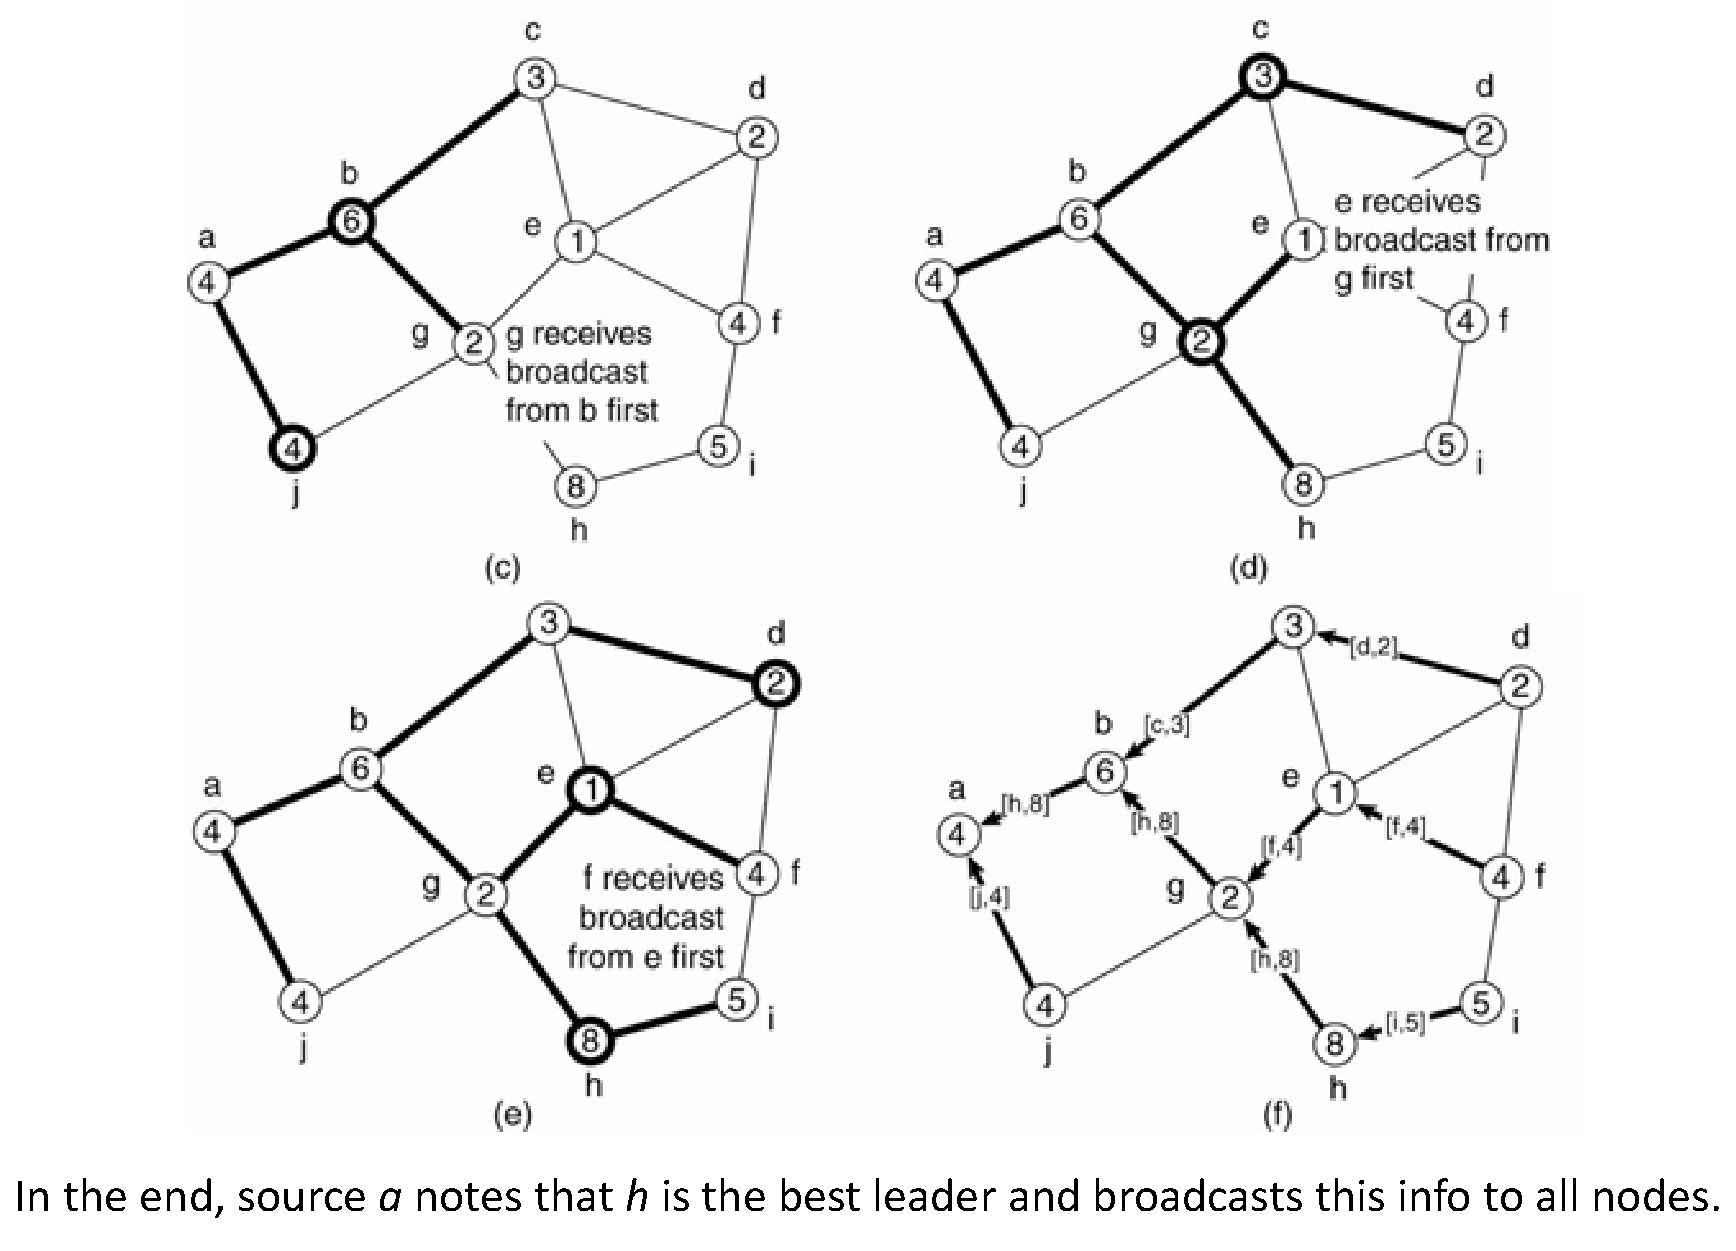
\includegraphics[width=1\linewidth]{example_general_topology_p2.pdf}
    \caption{Příklad činnosti algoritmu pro obecnou topologii, část 2.}
\end{figure}

\newpage

% 48
% VUT FIT MITAI
% MSZ 2021/2022
% Author: Vladimir Dusek
% Login: xdusek27

%%%%%%%%%%%%%%%%%%%%%%%%%%%%%%%%%%%%%%%%%%%%%%%%%%%%%%%%%%%%%%%%%%%%%%%%%%%%%%%%

% Path to figures
\graphicspath{{pdi/konzistentni_globalni_stav/figures}}

%%%%%%%%%%%%%%%%%%%%%%%%%%%%%%%%%%%%%%%%%%%%%%%%%%%%%%%%%%%%%%%%%%%%%%%%%%%%%%%%

\chapter{PDI -- Podmínky konsistentního globálního stavu distribuovaného systému.}

% Todo:
% - Chtelo by to pravdepodobne doplnit i algoritmy pro dosazeni konzistentniho stavu.

%%%%%%%%%%%%%%%%%%%%%%%%%%%%%%%%%%%%%%%%%%%%%%%%%%%%%%%%%%%%%%%%%%%%%%%%%%%%%%%%

\subsection{Zdroje}

\begin{compactitem}
    \item \path{04_Global_State_and_Snapshot.pdf}
    \item \path{PDI_2020-10-12.mp4}
\end{compactitem}

%%%%%%%%%%%%%%%%%%%%%%%%%%%%%%%%%%%%%%%%%%%%%%%%%%%%%%%%%%%%%%%%%%%%%%%%%%%%%%%%

\section{Úvod a kontext}

\paragraph*{Distribuovaný systém} Distribovaný systém je množina procesů $p_1, p_2, \dots, p_n$, které jsou propojeny komunikačními kanály. V~systému neexistuje žádná globální paměť ani globální hodiny. Procesy spolu komunikují pouze zasíláním zpráv skrze komunikačními kanály.

\paragraph*{Komunikační kanál} Komunikační kanál mezi procesy $p_i$ a $p_j$ značíme $C_{ij}$.

\paragraph*{Událost} Rozlišujeme tři typy událostí: interní událost procesu, zaslání zprávy a přijetí zprávy.

\paragraph*{Zpráva} Zpráva $m_{ij}$ značí zprávu zaslanou procesem $p_i$ procesu $p_j$. $send(m_{ij})$ značí odeslání zprávy a $recv(m_{ij})$ přijetí.

\paragraph*{Stav procesu} Lokální stav procesu $p_i$ značíme $LS_i$. Lokální stav je definován jako sekvence všech událostí, o~kterých proces $p_i$ ví. Nechť $e$ je libovolná událost, $e \in LS_i$ značí, že událost $e$ patří do lokálního stavu procesu $p_i$, $e \not\in LS_i$ značí, že událost $e$ nepatří do lokálního stavu procesu $p_i$.

\paragraph*{Stav komunikačního kanálu} Stav komunikačního kanálu $C_{ij}$ značíme $SC_{ij}$ a je definován množinou zpráv, které obsahuje. Pro kanál $C_{ij}$ můžeme definovat jeho stav na základě lokálních stavů procesů $LS_i$ a $LS_j$: $$
transit(LS_i, LS_j) = \{ m_{ij} \,|\, send(m_{ij}) \in LS_i \land rec(m_{ij}) \not\in LS_j \}
$$.

\section{Model komunikace}

\begin{compactitem}
    \item FIFO -- Komukační kanál funguje jako fronta zpráv \textit{first in}, \textit{first out}. Kanál tedy zachovává pořadí zpráv sám o~sobě.

    \item non-FIFO -- Komunikační kanál se chová jako datová struktura množina, do které odesílatel vkládá zprávy a příjemce je odebírá v~náhodném pořadí.

    \item Causal ordering (kauzální uspořádání) -- Systém, který podporuje kauzální doručení zpráv splňuje následující vlastnost. Pro jakékoliv dvě zprávy $m_{ij}$ a $m_{kj}$ platí, pokud $send(m_{ij}) \rightarrow send(m_{kj})$, pak i $recv(m_{ij}) \rightarrow recv(m_{kj})$.
\end{compactitem}

\section{Konzistentní globální stav}

\paragraph*{Globální stav} Globální stav distribuovaného systému je kolekce lokálních stavů procesů a komunikačních kanálů. $$
GS = \Big\{ \bigcup_{i} LS_i \,,\, \bigcup_{i, j} SC_{ij} \Big\}
$$.

\paragraph*{Časoprostorový diagram} Diagram pro vizualizaci komunikace procesů v~distribuovaném systému. Viz obrázek~\ref{48_example_cut} a~\ref{48_example_consistent_state}.

\paragraph*{Konzistentní globální stav} Konzistentní globální stav (\textit{snapshot}) je stav systému v~určitém časovém okamžiku. Lze si jej představit jako řez v~časoprostorovém diagramu, který rozděluje diagram na dvě části: minulost a budoucnost. Aby byl řez (globální stav) konzistentní, tak pokud je doručení nějaké zprávy v~minulosti, musí být v~minulosti i její odeslání. Formálně jde o~globální stav, který splňuje nálsedující podmínky:

$$
send(m_{ij}) \in LS_i \Rightarrow m_{ij} \in SC_{ij} \oplus recv(m_{ij}) \in LS_j
$$,

$$
send(m_{ij}) \not\in LS_i \Rightarrow m_{ij} \not\in SC_{ij} \land recv(m_{ij}) \not\in LS_j
$$.

\paragraph*{K čemu je \textit{snapshot}} \textit{Snapshot} lze využít např. pro tvorbu záloh systému nebo při zotavování systému po chybách.

\paragraph*{Jak lze \textit{snapshot} vytvořit} Absence globální sdílené paměti, globálních hodin a nepředvídatelná délka zpoždění v~odesílání zpráv v~distribuovaném systému činí problém vytváření snapshotů netriviálním. Způsob vytváření lze rozdělit do dvou kategorií: na základě algoritmů a na základě checkpointů.

\paragraph*{Problémy při zaznamenávání snapshotu} Jak rozlišit mezi zprávami, které mají být součástí snapshotu a které nikoliv?
\begin{compactitem}
    \item Zprávy, které jsou odeslány procesem před zaznamenáním svého  snapshotu, jsou zaznamenány do stavu.
    \item Zprávy, které jsouodeslány procesem po zaznamenání svého  snapshotu, nejsou zaznamenány do stavu.
\end{compactitem}

\noindent Jak rozpoznat okamžik, ve kterém má proces zaznamenat snapshot?
\begin{compactitem}
    \item Proces $p_j$ musí zaznamenat svůj snapshot před zpracováním zprávy $m_{ij}$, která byla poslána procesem $p_i$ po zaznamenání jeho snapshotu.
\end{compactitem}

\begin{figure}[H]
    \centering
    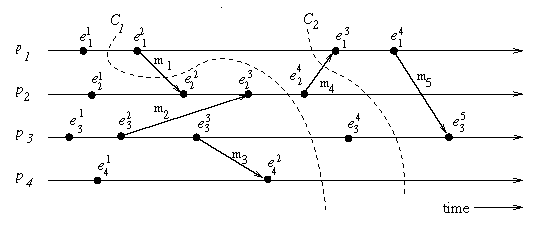
\includegraphics[width=1\linewidth]{example_cut.pdf}
    \caption{Příklad řezu v~časoprostorovém diagramu. Řez $C_1$ je nekonzistentní, kvůli zprávě $m_1$. Řez $C_2$ je konzistentní a zpráva $m_4$ je zachycena ve stavu kanálu $Ch_{21}$.}
    \label{48_example_cut}
\end{figure}


\begin{figure}[H]
    \centering
    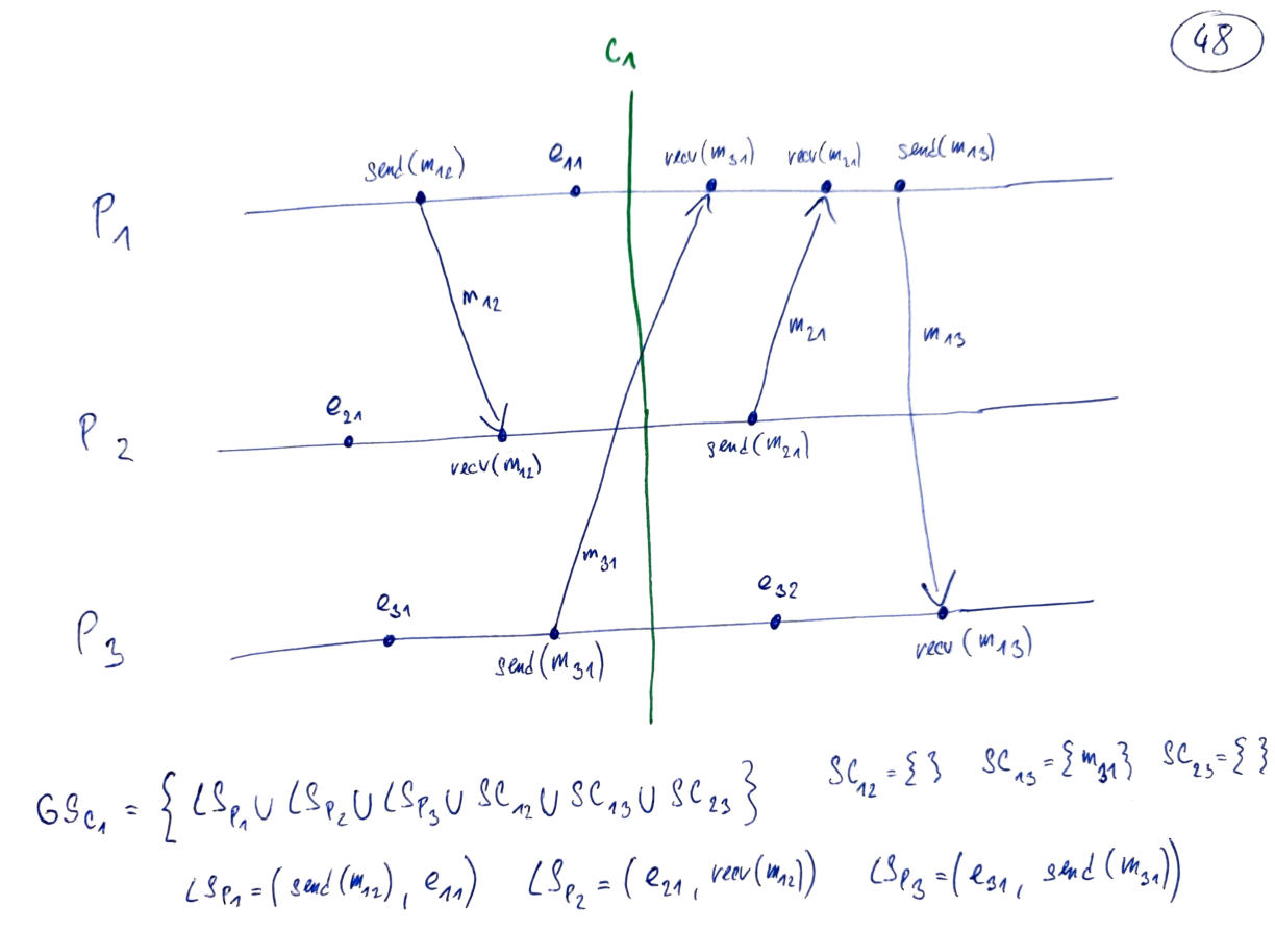
\includegraphics[width=1\linewidth]{example_consistent_state.pdf}
    \caption{Příklad konzistentního globální stavu formálně.}
    \label{48_example_consistent_state}
\end{figure}

\newpage

% 49
% VUT FIT MITAI
% MSZ 2021/2022
% Author: Vladimir Dusek
% Login: xdusek27

%%%%%%%%%%%%%%%%%%%%%%%%%%%%%%%%%%%%%%%%%%%%%%%%%%%%%%%%%%%%%%%%%%%%%%%%%%%%%%%%

% Path to figures
\graphicspath{{pdi/map_reduce/figures}}

%%%%%%%%%%%%%%%%%%%%%%%%%%%%%%%%%%%%%%%%%%%%%%%%%%%%%%%%%%%%%%%%%%%%%%%%%%%%%%%%

\chapter{PDI -- Principy distribuovaného zpracování MapReduce, průběh a jednotlivé operace distribuovaného výpočtu pomocí MapReduce, jeho implementace v~Apache Hadoop a Apache Spark.}

%%%%%%%%%%%%%%%%%%%%%%%%%%%%%%%%%%%%%%%%%%%%%%%%%%%%%%%%%%%%%%%%%%%%%%%%%%%%%%%%

\section{Zdroje}

\begin{compactitem}
    \item Předmět: Prostředí distribuovaných aplikací (PDI)
    \item Přednáška:
    \begin{compactitem}
        \item 9) Programovací model MapReduce a Apache Hadoop
        \item 10) Distribuované souborové systémy
        \item 11) Apache Spark
    \end{compactitem}
    \item Záznam:
    \begin{compactitem}
        \item 2020-11-16
        \item 2020-11-23
    \end{compactitem}
\end{compactitem}

%%%%%%%%%%%%%%%%%%%%%%%%%%%%%%%%%%%%%%%%%%%%%%%%%%%%%%%%%%%%%%%%%%%%%%%%%%%%%%%%

\section{Úvod a kontext}

\paragraph*{OLTP} OLTP (\textit{Online Transactional Processing}, provozní databáze, systémy pro online zpracování transakcí) jsou standardní databázové systémy s~pevnou strukturou dat definovou pomocí databázového schématu. Jsou navrženy a optimalizovány pro chod provozních aplikací s~primárním cílem zajistit rychlý a souběžný přístup k~datům. To vyžaduje transakční zpracování, řízení souběžnosti a techniky obnovy (rollback), které zaručují konzistenci dat. Díky těmto vlastnostem mají OLTP databáze špatný výkon při provádění složitých dotazů, které potřebují spojit mnoho relačních tabulek dohromady nebo agregovat velké objemy dat. Kromě toho obsahují typicky podrobná data a neobsahují historická data, která jsou při datové analýze potřeba.

\paragraph*{OLAP} OLAP (\textit{Online Analytical Processing}, online analytické zpracování) je databázové paradigma specificky zaměřené na dotazy, zejména na analytické dotazy. Používají se zde jiné techniky indexování a optimalizace dotazů. Normalizace není pro toto paradigma žádoucí, protože rozděluje databázi na mnoho tabulek. Složité dotazy v~takovém případě vyžadují rekonstrukci dat a s~tím spojený vysoký počet spojování tabulek. Pracuje se s~tzv. multidimenzionálními kostkami, avšak v~pozadí jsou stále relační databáze.

\paragraph*{NoSQL} Potřeba ukládat proudy dat (zpracovávané v~reálném čase bez možnosti pozastavení), obrázky, multimédia, velké JSON soubory, \dots, vedla ke vzniku NoSQL databází. NoSQL databáze používají jiné prostředky než tabulková schémata tradiční relační databáze. Často jde o~\uv{hloupé}, nestrukturované uložiště klíč-hodnota.

\paragraph*{BigData} Velká, nestrukturovaná (různorodá), rychle rostoucí data, která není možné uložit ani zpracovávat běžnými přístupy (na jednom uzlu, jedním uzlem). Produkují je např.: IoT senzory, sociální sítě, chatovací aplikace, webové vyhledávače, \dots \, Pro jejich zpracování je nutné využít distribuované systémy (pro uložení i zpracování).

\paragraph*{Distribuované zpracování dat} Distribuované zpracování dat je zpracování velkých dat (\textit{big data}) pomocí distribuovaných systémů. To s~sebou přináší problémy. Jak zaručit vhodnou distribuci dat a výpočtu mezi uzly? Jak řešit nespolehlivost a výpadky uzlů? Jak a kam zajistit doručení výsledků výpočtu? \dots

%%%%%%%%%%%%%%%%%%%%%%%%%%%%%%%%%%%%%%%%%%%%%%%%%%%%%%%%%%%%%%%%%%%%%%%%%%%%%%%%

\section{MapReduce}

Algoritmy pro indexování webových stránek (Page Rank) přestávaly být udržitelné, bylo potřeba zvýšit jejich škálovatelnost. Google vydal příspěvek \uv{MapReduce: Simplified Data Processing on Large Clusters}, kde bylo představeno paradigma MapReduce. Jde o~paradigma distribuovaného výpočtu založené na funkcích \textit{map} a \textit{reduce} z~funcionálního programování.

\paragraph*{Map} Funkce \textit{map} má ve funkcionálním programování 2 vstupní parametry a vrací seznam hodnot. První parametr je unární operátor (nebo funkce fungující jako unární operátor) a druhý je seznam hodnot. Výstupní seznam je spočítán jako aplikace unárního operátoru na vstupní seznam. Příklad:
$$
map(square, [1, 2, 3, 4]) = [1, 4, 9, 16]
$$.
V~paradigmata MapReduce \textit{map} vrací data jako seznam dvojic klíč-hodnota, přesněji: $$
map((key, value)) \rightarrow [(key, value)]
$$.

\paragraph*{Reduce} Funkce \textit{reduce} má ve funkcionálním programování 2 vstupní parametry a vrací jednu hodnotu. První parametr je binární operátor (nebo funkce fungující jako binární operátor) a druhý je seznam hodnot. Výstupní hodnota je spočítána jako postupná aplikace binárního operátoru na všechny hodnoty ve vstupním seznamu. Příklad:
$$
reduce(+, [1, 4, 9, 16]) = 30
$$.
V~paradigmata MapReduce \textit{reduce} bere na vstupu klíč a seznam hodnot a vrací opět seznam dvojic klíč-hodnota, přesněji: $$
reduce(key, [value]) \rightarrow [(key, value)]
$$.

\bigskip\noindent\begin{minipage}{\linewidth}
\begin{lstlisting}[language=Python, caption={Příklad implementace funkcí \textit{map} a \textit{reduce} v~paradigmatu MapReduce pro počítání četnosti slov ve vstupu v~Pythonu.}]
def map(input_key: str, input_value: str) -> list[tuple[str, int]]:
    # input_key - document name
    # input_value - document content (etc. line)
    result = []
    for word in input_value.split(' '):
        result.append((word, 1))
    return result

def reduce(input_key: str, input_value: list[int]) -> tuple[str, int]:
    result = 0
    for val in input_value:
        result += value
    return (input_key, result)
\end{lstlisting}
\end{minipage}

\begin{figure}[H]
    \centering
    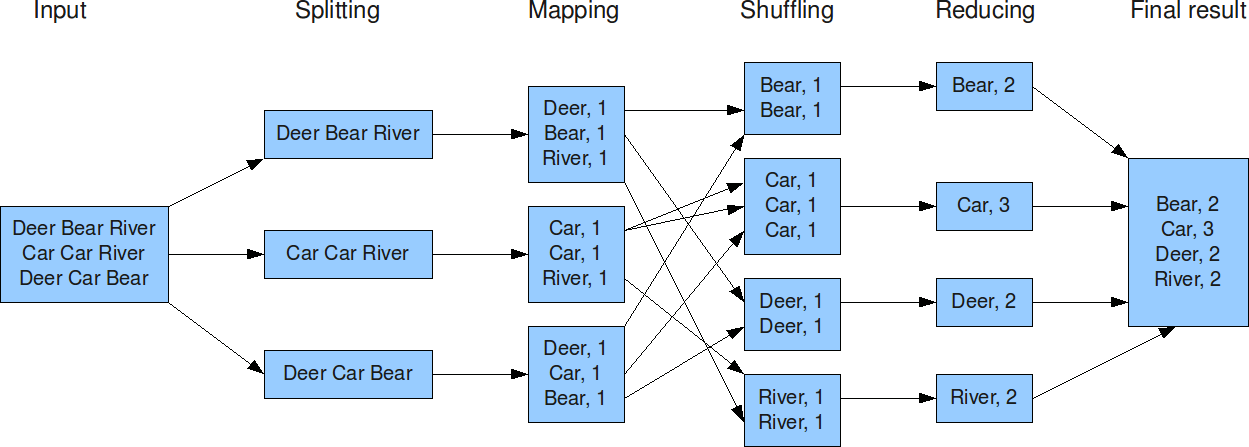
\includegraphics[width=1\linewidth]{map_reduce_example.png}
    \caption{Úloha počítání četnosti slov v~paradigmatu MapReduce v~diagramu.}
    \label{49_map_reduce_example}
\end{figure}

\paragraph*{Průběh MapReduce} Celý MapReduce probíhá v~několika krocích, viz obrázek~\ref{49_map_reduce_example}.
\begin{compactenum}
    \item Input -- Přípravený vstup pro distribuovaný výpočet (např. soubory ve virtuálním distribuovaném souborovém systému, viz dále HDFS).
    \item Splitting -- Rozdělení vstupu na části, které budou přiděleny jednotlivým uzlům. Může být výchozí (např. rozdělení textového souboru po řádcích) nebo definováno uživatelem.
    \item Mapping -- Každý uzel aplikuje funkci \textit{map} na svoji přidělenou část. Uživatel definuje jak má funkce \textit{map} vypadat.
    \item Shuffling (také Grouping, Partitioning, Comparing)-- Výpočetní uzly si mezi sebou vymění hodnoty, které spočítaly, na základě klíče. Tento krok zařižuje platforma pro distribuovaný výpočet sama o~sobě, typicky na základě hashů klíčů. Tento krok je většinou \textit{bottleneck}.
    \item Reducing -- Každý uzel zapojený do tohoto kroku (často je v~tomto kroku potřeba méně uzlů, než v~kroku mapping) aplikuje funkci \textit{reduce} na svoji přidělenou část. Uživatel definuje jak má funkce \textit{reduce} vypadat.
    \item Final Result -- Finální výsledek (např. zapsán do do virtuálního distribuovaného souborového systému, viz dále HDFS).
\end{compactenum}

\begin{figure}[H]
    \centering
    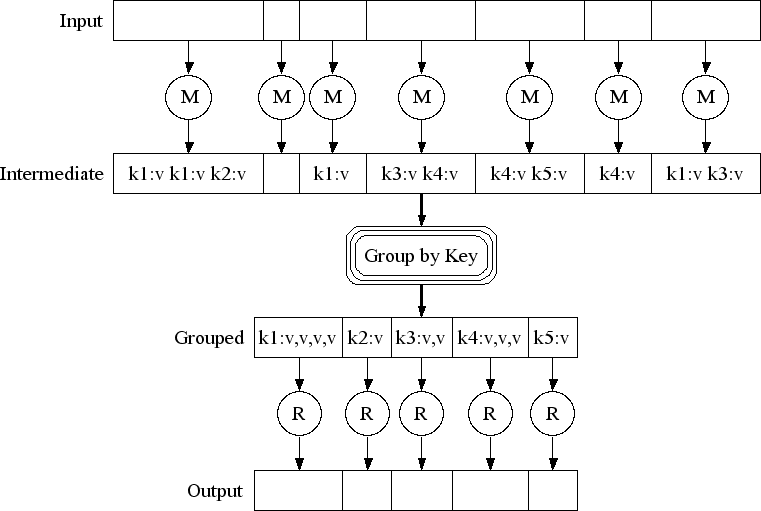
\includegraphics[width=1\linewidth]{map_reduce_general_p1.png}
    \caption{Výpočet MapReduce v~obecném schématu.}
\end{figure}

\paragraph*{Combiner} Optimalizační krok, jde o~\uv{jakési} provedení operace \textit{reduce} už ve fázi \textit{map} (každým uzlem). Tím je snížen počet mezivýsledků ve fázi Shuffling. Typicky funkce \textit{combine} je stejná jako \textit{reduce}.

\paragraph*{Virtuální distribuovaný souborový systém} Pro realizaci distribuovaného výpočtu je rovněž potřeba distribuovaný souborový systém (DFS). Ten je typicky realizován jako virtuální souborový systém nad jednotlivými souborovými systémy uzlů. Např.: GFS -- Google File System, HDFS -- Hadoop File System (viz dále). DFS obsahuje data samotná (\textit{data nodes}) a metadata o~tom, která data jsou na jakých uzlech (\textit{name nodes}).

\begin{figure}[H]
    \centering
    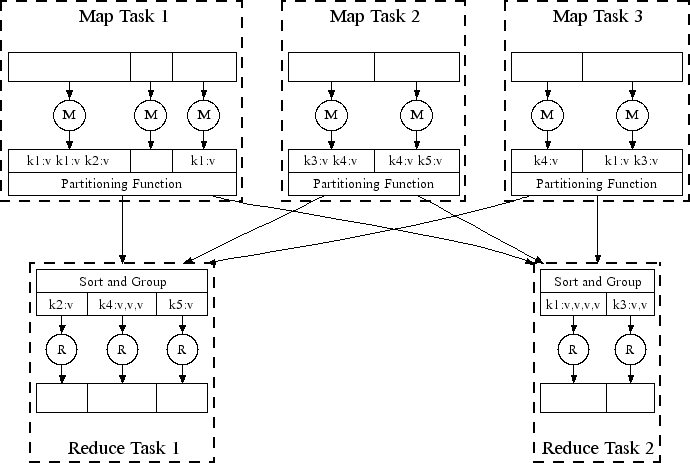
\includegraphics[width=1\linewidth]{map_reduce_general_p2.png}
    \caption{Výpočet MapReduce v~obecném schématu a rozdělením práce na jednotlivé uzly (uzel je typicky víceprocesorový).}
\end{figure}

%%%%%%%%%%%%%%%%%%%%%%%%%%%%%%%%%%%%%%%%%%%%%%%%%%%%%%%%%%%%%%%%%%%%%%%%%%%%%%%%

\section{Apache Hadoop}

% Todo:
% - Dale by se dalo mluvit podrobneji o implementaci, viz slajd 26 (job tracker, task tracker).

Apache Hadoop je \textit{open-source} implementace MapReduce paradigmatu vyvíjená Apache Software Foundation. Jde o~implementaci v~Jave, ta je vhodná, jelikož díky JVM (Java Virtual Machine) je spouštění uživatel definovaných funkcí \textit{map} a \textit{reduce} snadné.

\paragraph*{Hadoop MapReduce} -- Implementace MapReduce paradigma. Data jsou čtena a ukládána na HDFS (včetně mezivýsledků). To znamená, můžeme pracovat v~podstatě neomezenými daty, ale ukládání a načítání výpočet zpomalují.\footnote{\textit{Nebylo přednášeno podrobněji, pravděpodobně stačí princip obecného MapReduce, který byl vysvětlen v~předchozí sekci.}}.

\paragraph*{HDFS} HDFS (\textit{Hadoop Distribute File System}) je virtuální distribuovaný souborový systém. Standardní soubor je rozdělen na datové bloky které jsou distribuovány na různé datové uzly. Architektura HDFS se skládá ze dvou typů uzlů~--~Name Node a Data Node. Name Node obsahuje alokační tabulku pro souborový systém. Ví které datové bloky patří kterému souboru a kde jsou uloženy. Obsahuje další metadata jako názvy souborů, cesty, \dots \, Data Node obsahuje datové bloky. Typicky redundance a replikace, počítá se s~možným selháním uzlů. Pro \textbf{čtení dat} se klient zeptá Name Nodu na konkrétní soubor v~HDFS. Name Node vrátí metadata o~souboru, na jakých Data Nodech se vyskytuje. Klient požádá příslušné Data Nody, ty mu pošlou data, která se na klientovi \uv{poskládají} do výsledného souboru. Pro \textbf{zápis dat} se klient zeptá Name Nodu, kam by měl zapisovat. Klient zapíše na příslušný Data Node. Data Node poté vyřeší replikace s~dalšími uzly.

\paragraph*{Hadoop YARN} Hadoop YARN je plánovač (\textit{scheduler}). Plánuje výpočet tak, aby proběhl co nejlepším způsobem na konkrétnbí distribuované architektuře. Plánovač má obecné obecné rozhraní a Hadoop YARN lze nahradit za jiný.

\paragraph*{Hadoop Common} Hadoop Common jsou další knihovny a ovladače pro klienty.

\paragraph*{Další nástroje} Nad Apache Hadoop existuje mnoho dalších nástrojů. Apache Pig pro \textit{high level} programování map-reduce úloh. Apache Hive pro pro dolování dat nad Apache Hadoop. Apache HBase jako distribuovaná databáze nad Apache Hadoop, \dots

%%%%%%%%%%%%%%%%%%%%%%%%%%%%%%%%%%%%%%%%%%%%%%%%%%%%%%%%%%%%%%%%%%%%%%%%%%%%%%%%

\section{Apache Spark}

Apache Spark je \textit{open-source} nástroj pro distribuované zpracování rozsáhlých dat vyvíjený Apache Software Foundation. Hlavní cíl je zvýšení rychlosti. Spark na to jde přesunutím co nejvíce výpočtů do operační paměti jednotlivých uzlů a tím pádem zminimalizovat počet zápisů a čtení z~DFS (snaha odstranit \textit{bottleneck} v~kroku shuffling u~Hadoopu). Tím ale vzniká jiný problém, a sice výpadek uzlu znamená, že data jsou ztraceny.

\begin{figure}[H]
    \centering
    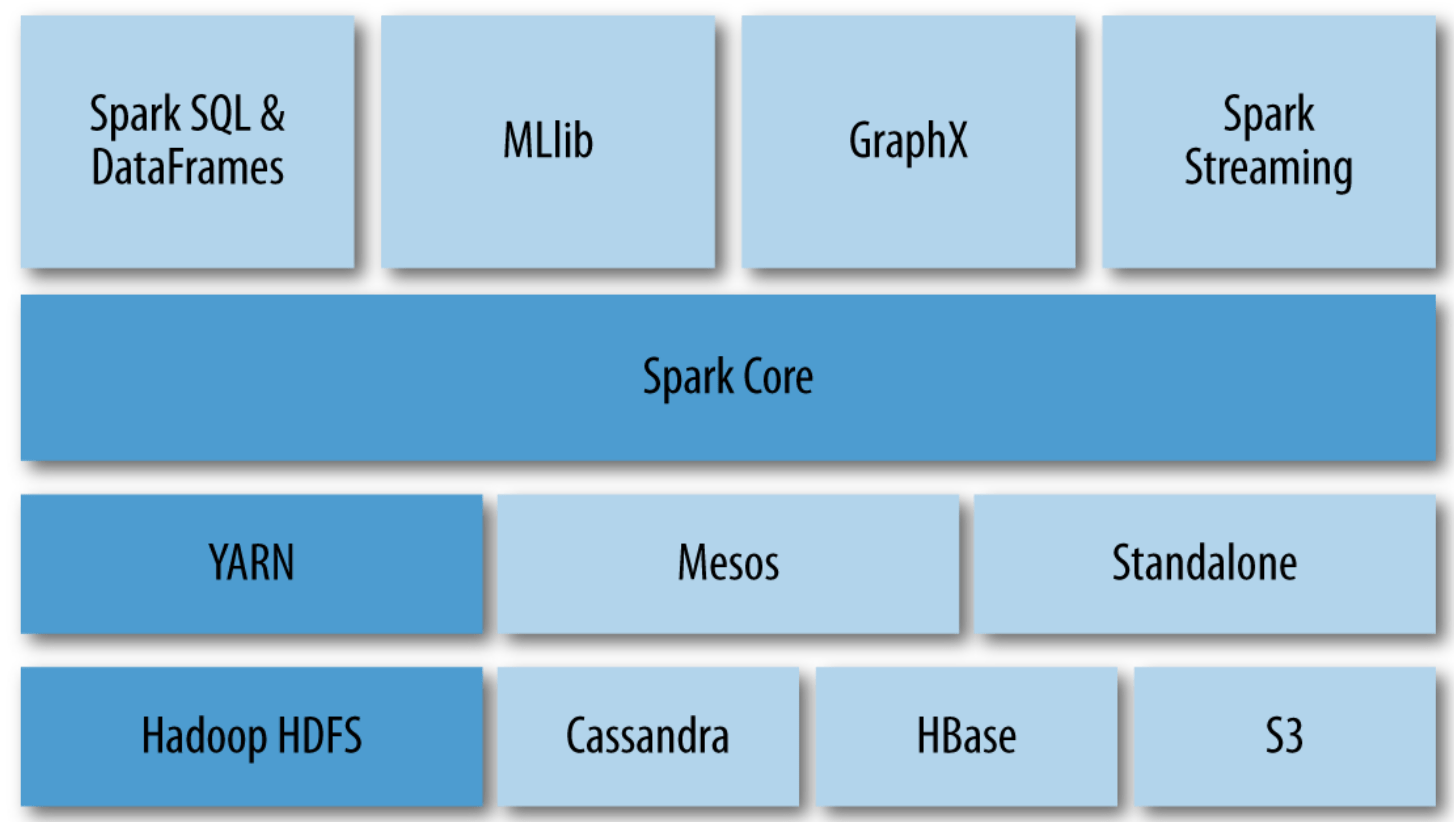
\includegraphics[width=0.75\linewidth]{spark.png}
    \caption{Architektura Apache Spark. Hlavní je Spark Core, zbytek funguje na systému pluginů a může používat HDFS, Hadoop YARN a Hadoop Common.}
\end{figure}

% todo: pokracovani, 30 min prednaska

\paragraph*{Resilient Distributed Dataset} Resilient Distributed Dataset (RDD) je základní datová struktura Sparku. Jedná se o~typované kolekce n-tic, které jsou neměnné (\textit{read only}). Vstup je transformován na RDD a každá operace je pak transformace jednoho RDD na jiné.
$$
RDD_1 \rightarrow map() \rightarrow RDD_2 \rightarrow reduce() \rightarrow RDD_3
$$

\paragraph*{Strategie vyhodnocování} Spark uplatňuje strategii vyhodnocování \textit{lazy evaluation}. Vyhodnocování výrazu je odkládáno až do doby, dokud není potřeba jeho hodnota. Zabraňuje opakovanému vyhodnocování. Je vyhodnocována pouze ta část, která je potřeba. RDD funguje jako abstraktní datová struktura, nemusí obsahovat data uvnitř, ale pouze předpis jak data získat a získá je, až když jsou potřeba.

\paragraph*{Struktura výpočtu} Struktura výpočtu odpovídá orientovanému acyklickému grafu (DAG, \textit{Directed Acyclic Graph}). Uzly jsou RDD a hrany jsou transformace. DAG je znám i dalším uzlům, takže pokud nastane výpadek uzlu a výpočet je ztracen, může být uzel snadno zastoupen.

\paragraph*{Klíčové vlastnosti} Klíčové vlastnosti Sparku jsou \textit{lazy evaluation}, \textit{in-memmory} a \textit{parallel computing}.

\begin{figure}[H]
    \centering
    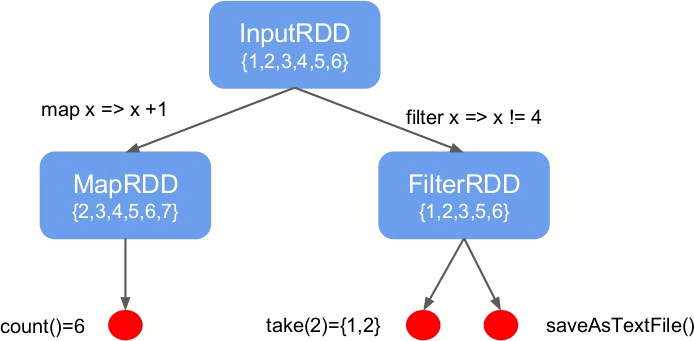
\includegraphics[width=0.85\linewidth]{spark_example.png}
    \caption{Příklad výpočtu v~Apache Spark.}
\end{figure}

\newpage

% 50
% VUT FIT MITAI
% MSZ 2021/2022
% Author: Vladimir Dusek
% Login: xdusek27

%%%%%%%%%%%%%%%%%%%%%%%%%%%%%%%%%%%%%%%%%%%%%%%%%%%%%%%%%%%%%%%%%%%%%%%%%%%%%%%%

% Path to figures
\graphicspath{{kry/symetricka_kryptografie/figures}}

%%%%%%%%%%%%%%%%%%%%%%%%%%%%%%%%%%%%%%%%%%%%%%%%%%%%%%%%%%%%%%%%%%%%%%%%%%%%%%%%

\chapter{KRY -- Symetrická kryptografie. Vlastnosti, vlastnosti bezpečného algoritmu, délka klíče, útok silou, příklady symetrických algoritmů, Feistelovy šifry, DES, režimy činnosti, proudové šifry.}

% Todo: 3DES, AES (ptali se na to)

%%%%%%%%%%%%%%%%%%%%%%%%%%%%%%%%%%%%%%%%%%%%%%%%%%%%%%%%%%%%%%%%%%%%%%%%%%%%%%%%

\section{Zdroje}

\begin{compactitem}
    \item Předmět: Kryptografie (KRY)
    \item Přednáška:
    \begin{compactitem}
        \item 3) Symetrická kryptografie. Vlastnosti, vlastnosti bezpečného algoritmu, délka klíče, útok silou.
        \item 4) Příklady symetrických algoritmů, Feistelovy šifry, DES, struktura, činnost, slabiny, režimy činnosti.
        \item 5) Typické aplikace symetrické kryptografie.
    \end{compactitem}
    \item Záznam:
    \begin{compactitem}
        \item 2021-02-22
        \item 2021-03-01
        \item 2021-03-08
    \end{compactitem}
\end{compactitem}

%%%%%%%%%%%%%%%%%%%%%%%%%%%%%%%%%%%%%%%%%%%%%%%%%%%%%%%%%%%%%%%%%%%%%%%%%%%%%%%%

\section{Úvod a kontext}

\paragraph*{Kryptografie} Kryptografie (šifrování) je věda o~metodách utajování smyslu zpráv převodem do podoby, která je čitelná jen se speciální znalostí.

\paragraph*{Kryptoanalýza} Kryptoanalýza je věda zabývající se metodami získávání obsahu šifrovaných informací bez přístupu k~tajným informacím, které jsou za normálních okolností potřeba, tzn. především k~tajnému klíči.

\paragraph*{Kryptologie} Jeden výraz pro kryptografii a kryptoanalýzu.

\paragraph*{Caesarova šifra} Princip Caesarovy šifry je založen na tom, že všechna písmena zprávy jsou během šifrování zaměněna za písmeno, které se abecedně nachází o~pevně určený počet míst dále (tj. posun je pevně zvolen). Caesarova šifra spadá do kategorie substitučních šifer (stejný znak je při více vyskytech vždy zašifrován na stejný znak).

\paragraph*{Vigenerova šifra} Rozšíření Caesarovy šifry, klíč je delší než 1 znak. Klíč je řetězec, který reprezentuje posuny. V~případě že vstup je delší než klíč, je klíč perioricky opakován. Vigenerova šifra spadá do kategorie polyalfabetických substitučních šifer (stejný znak může být při více výskytech zašifrován na jiný znak).

\paragraph*{Vernamova šifra (\textit{One Time Pad})} Vernamova šifra spadá do kategorie polyalfabetických substitučních šifer a je i dnes nerozluštitelná pokud: \begin{compactitem}
    \item klíč je delší než vstupní text,
    \item klíč se nepoužije opakovaně,
    \item klíč je náhodný.
\end{compactitem}

\begin{figure}[H]
    \centering
    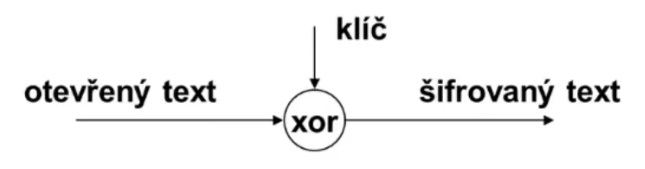
\includegraphics[width=0.5\linewidth]{vernam.png}
    \caption{Vernamova šifra.}
\end{figure}

\paragraph*{Autoklíč (\textit{autokey})} Šifrování klíčem a když vstupní text je delší než klíč, tak se pokračuje šifrováním otevřeným nebo šifrovaným textem. Lze použít u~Vigenerovy nebo Vernamovy šifry.

\paragraph*{Symetrická kryptografie} Algoritmy používají k~šifrování i dešifrování stejný klíč. Výhodou symetrických šifer je jejich nízká výpočetní náročnost. Asymetrické šifry mohou být i stotisíckrát pomalejší. Nevýhodou je nutnost sdílení tajného klíče, takže jedna strana musí klíč vygenerovat a potom ho bezpečným způsobem předat druhé straně.

\paragraph*{Typy útoků} \begin{compactitem}
    \item Ciphertext Only Attack (COA) -- Útočník zná pouze zašifrovaný text a snaží se zjistit klíč nebo otevřený text. Nejčastěší případ.
    \item Known Plaintext Attack (KPA) -- Útočník zná zašifrovaný text a otevřený text a snaží se zjistit klíč.
    \item Chosen Plaintext Attack (CPA) -- Útočník zná to co v~KPA a navíc si text může zvolit.
\end{compactitem}

\paragraph*{Útok silou} Pří útoku silou (\textit{brute force}) zkouší útočník všechny teoreticky možné klíče, dokud nenajde ten správný.

\begin{figure}[H]
    \centering
    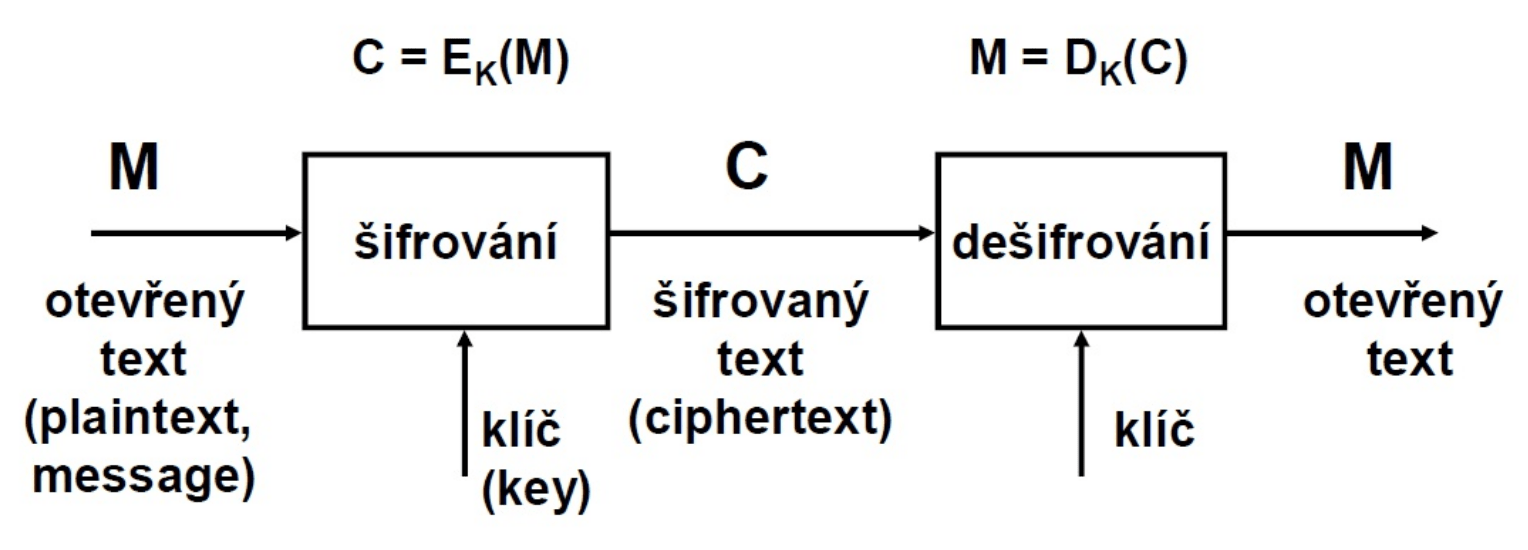
\includegraphics[width=0.75\linewidth]{kryptografie.png}
    \caption{Princip kryptografie, podle typu klíčů dělíme na symetrickou (tajný klíč) a asymetrickou (veřejný klíč, soukromý klíč).}
\end{figure}

\paragraph*{Bezpečný algoritmus} V~moderní kryptografii je nepřijatelné utajování algoritmů (\textit{security by obscurity})~--~předpokládáme, že útočník zná šifrovací algoritmus. Bezpečnost musí záviset pouze na utajení klíče (Kerckhoffuv princip, \textit{security by design}). Symetrický algoritmus je považován za bezpečný, pokud neexistuje rychlejší útok než útok silou.

\paragraph*{Délka klíče} Dnes je považováno 80 bitů a více za dostatečné. Typicky se délka zaokrouhluje na mocninu 2 (typicky 128b). Klíče symetrických algoritmů jsou kratší než asymetrických. Konkrétně: DES -- 56b, 3DES -- 112, AES -- variabilní.

\paragraph*{Využití} Symetrická kryptografie je vhodná pro šifrování většího objemu dat. Narozdíl od asymetrické, která je pro tento účel příliš pomalá. Proto např. HTTPS využívá asymetrickou kryptografii pro výměnu symetrických klíčů a poté symetrickou kryptografii pro šifrování provozu.

\paragraph*{Vlastnosti moderní kryptografie} Symetrická kryptografie zaručuje všechny následující, kromě nepopiratelnosti~--~více entit má k~dispozici klíč. \begin{compactitem}
    \item Důvernost -- Utajení informace. Bez znalosti klíče, není možné data číst.

    \item Autentizace -- Prokázání, že zprávu skutečně poslal odesílatel a nikoliv útočník, který se za odesílatele vydává.

    \item Integrita -- Prokázání, že nikdo nemohl data po cestě od odesílatele k~příjemci změnit. Ochrana proti neoprávněné, neodhalené modifikaci zprávy.

    \item Nepopiratelnost -- Pokud odesílatel data poslal, nemůže tuto skutečnost popřít.
\end{compactitem}

%%%%%%%%%%%%%%%%%%%%%%%%%%%%%%%%%%%%%%%%%%%%%%%%%%%%%%%%%%%%%%%%%%%%%%%%%%%%%%%%

\section{Blokové šifry}

Blokové šifry šifrují data po blocích pevně stanovené délky (64b, 128b, 256b, \dots). Pokud je dat více, rozdělí se na více bloků, přičemž do zbylého místa v~posledním je umístěno zarovnání \textit{padding} (informace o~délce zarovnání může být obsažena v~posledním bytu). Příklady blokových šifer: \begin{compactitem}
    \item Feistelova šifra (spíše princip)
    \item Data Encryption Standard (DES)
    \item Triple Data Encryption Algorithm (3DES)
    \item International Data Encryption Algorithm (IDEA)
    \item Blowfish
    \item Tiny Encryption Algorithm (TEA)
    \item Advanced Encryption Standard (AES)
\end{compactitem}

\begin{figure}[H]
    \centering
    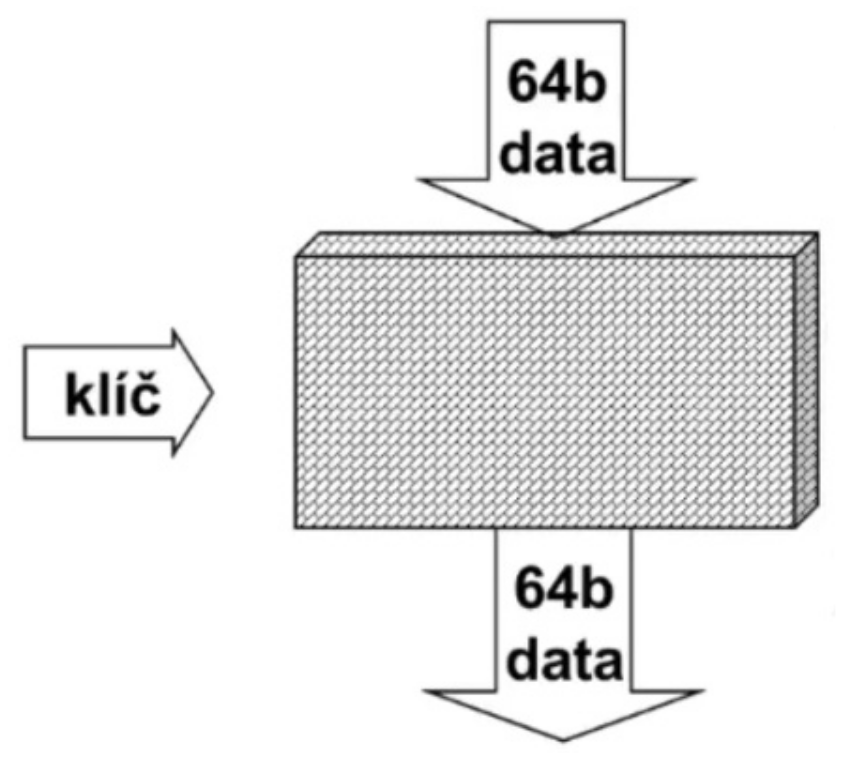
\includegraphics[width=0.35\linewidth]{symmetric_cryptography_blocks.png}
    \caption{Princip blokových šifer.}
\end{figure}

\subsection{Feistelova šifra}

Feistelova šifra (Feistelův princip) je koncept šifrování, který konkrétní algoritmy využívají. Jedná se o~substituční-permutační síť. Vstupní blok je rozdělen na dvě poloviny $L$ a $R$, výpočet výstupu pak vypadá následovně.

\begin{equation}
    L_i = R_{i-1}
\end{equation}

\begin{equation}
    R_i = L_{i-1} \oplus F(R_{i-1}, K_i)
\end{equation}

\paragraph*{Funkce F} $F$ je funkce, na kterou Feistelova šifra neklade žádné požadavky. Jednotlivé algoritmy, využívající Festelovu šifru, funkci samy definují. Požadavky na funkci $F$, aby algoritmus byl bezpečný: \begin{compactitem}
    \item skrytí vlastností zprávy;
    \item skrytí vlastností zprávy.
\end{compactitem}

\paragraph*{Subklíč} K~je tzv. subklíč, který je generován typicky nějakým pseudonáhodným generátorem na základě inicializačního klíče (hlavní).

\paragraph*{Dešifrování} Dešifrování se provádí stejným způsobem, pouze pořadí subklíčů je opačné.

\begin{figure}[H]
    \centering
    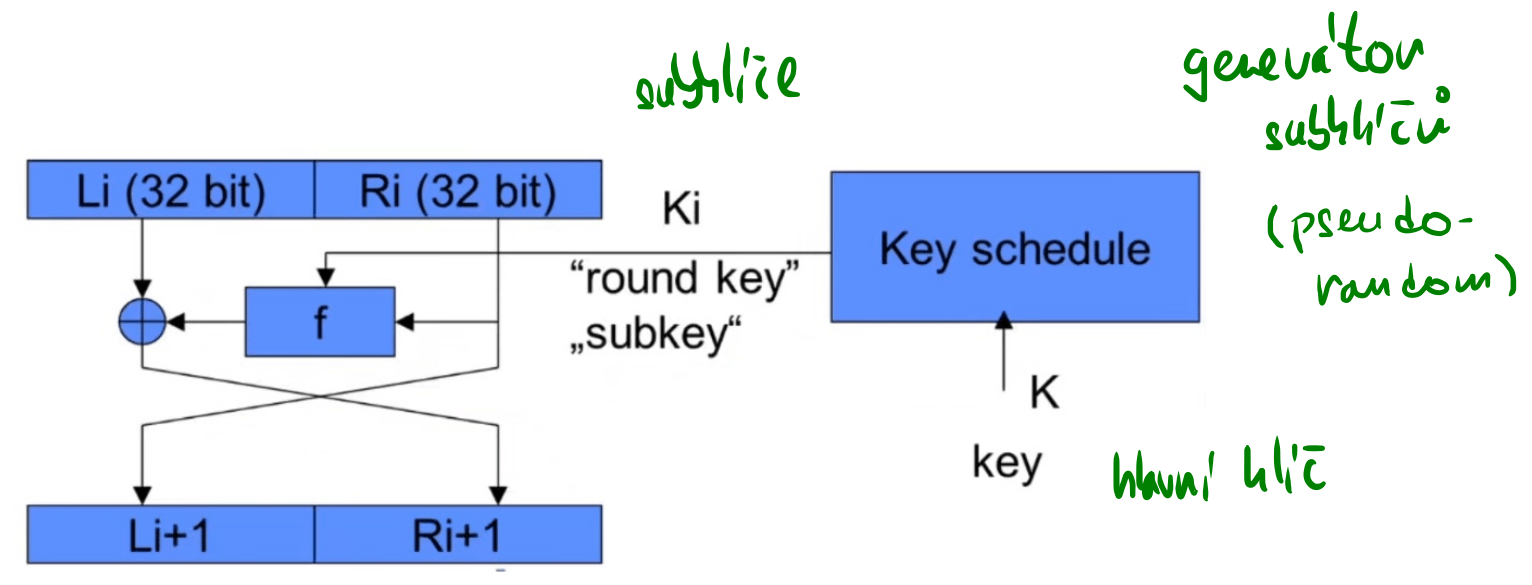
\includegraphics[width=1\linewidth]{feistel.png}
    \caption{Jeden krok opakování (Feistelův krok) vizuálně.}
\end{figure}

\begin{figure}[H]
    \centering
    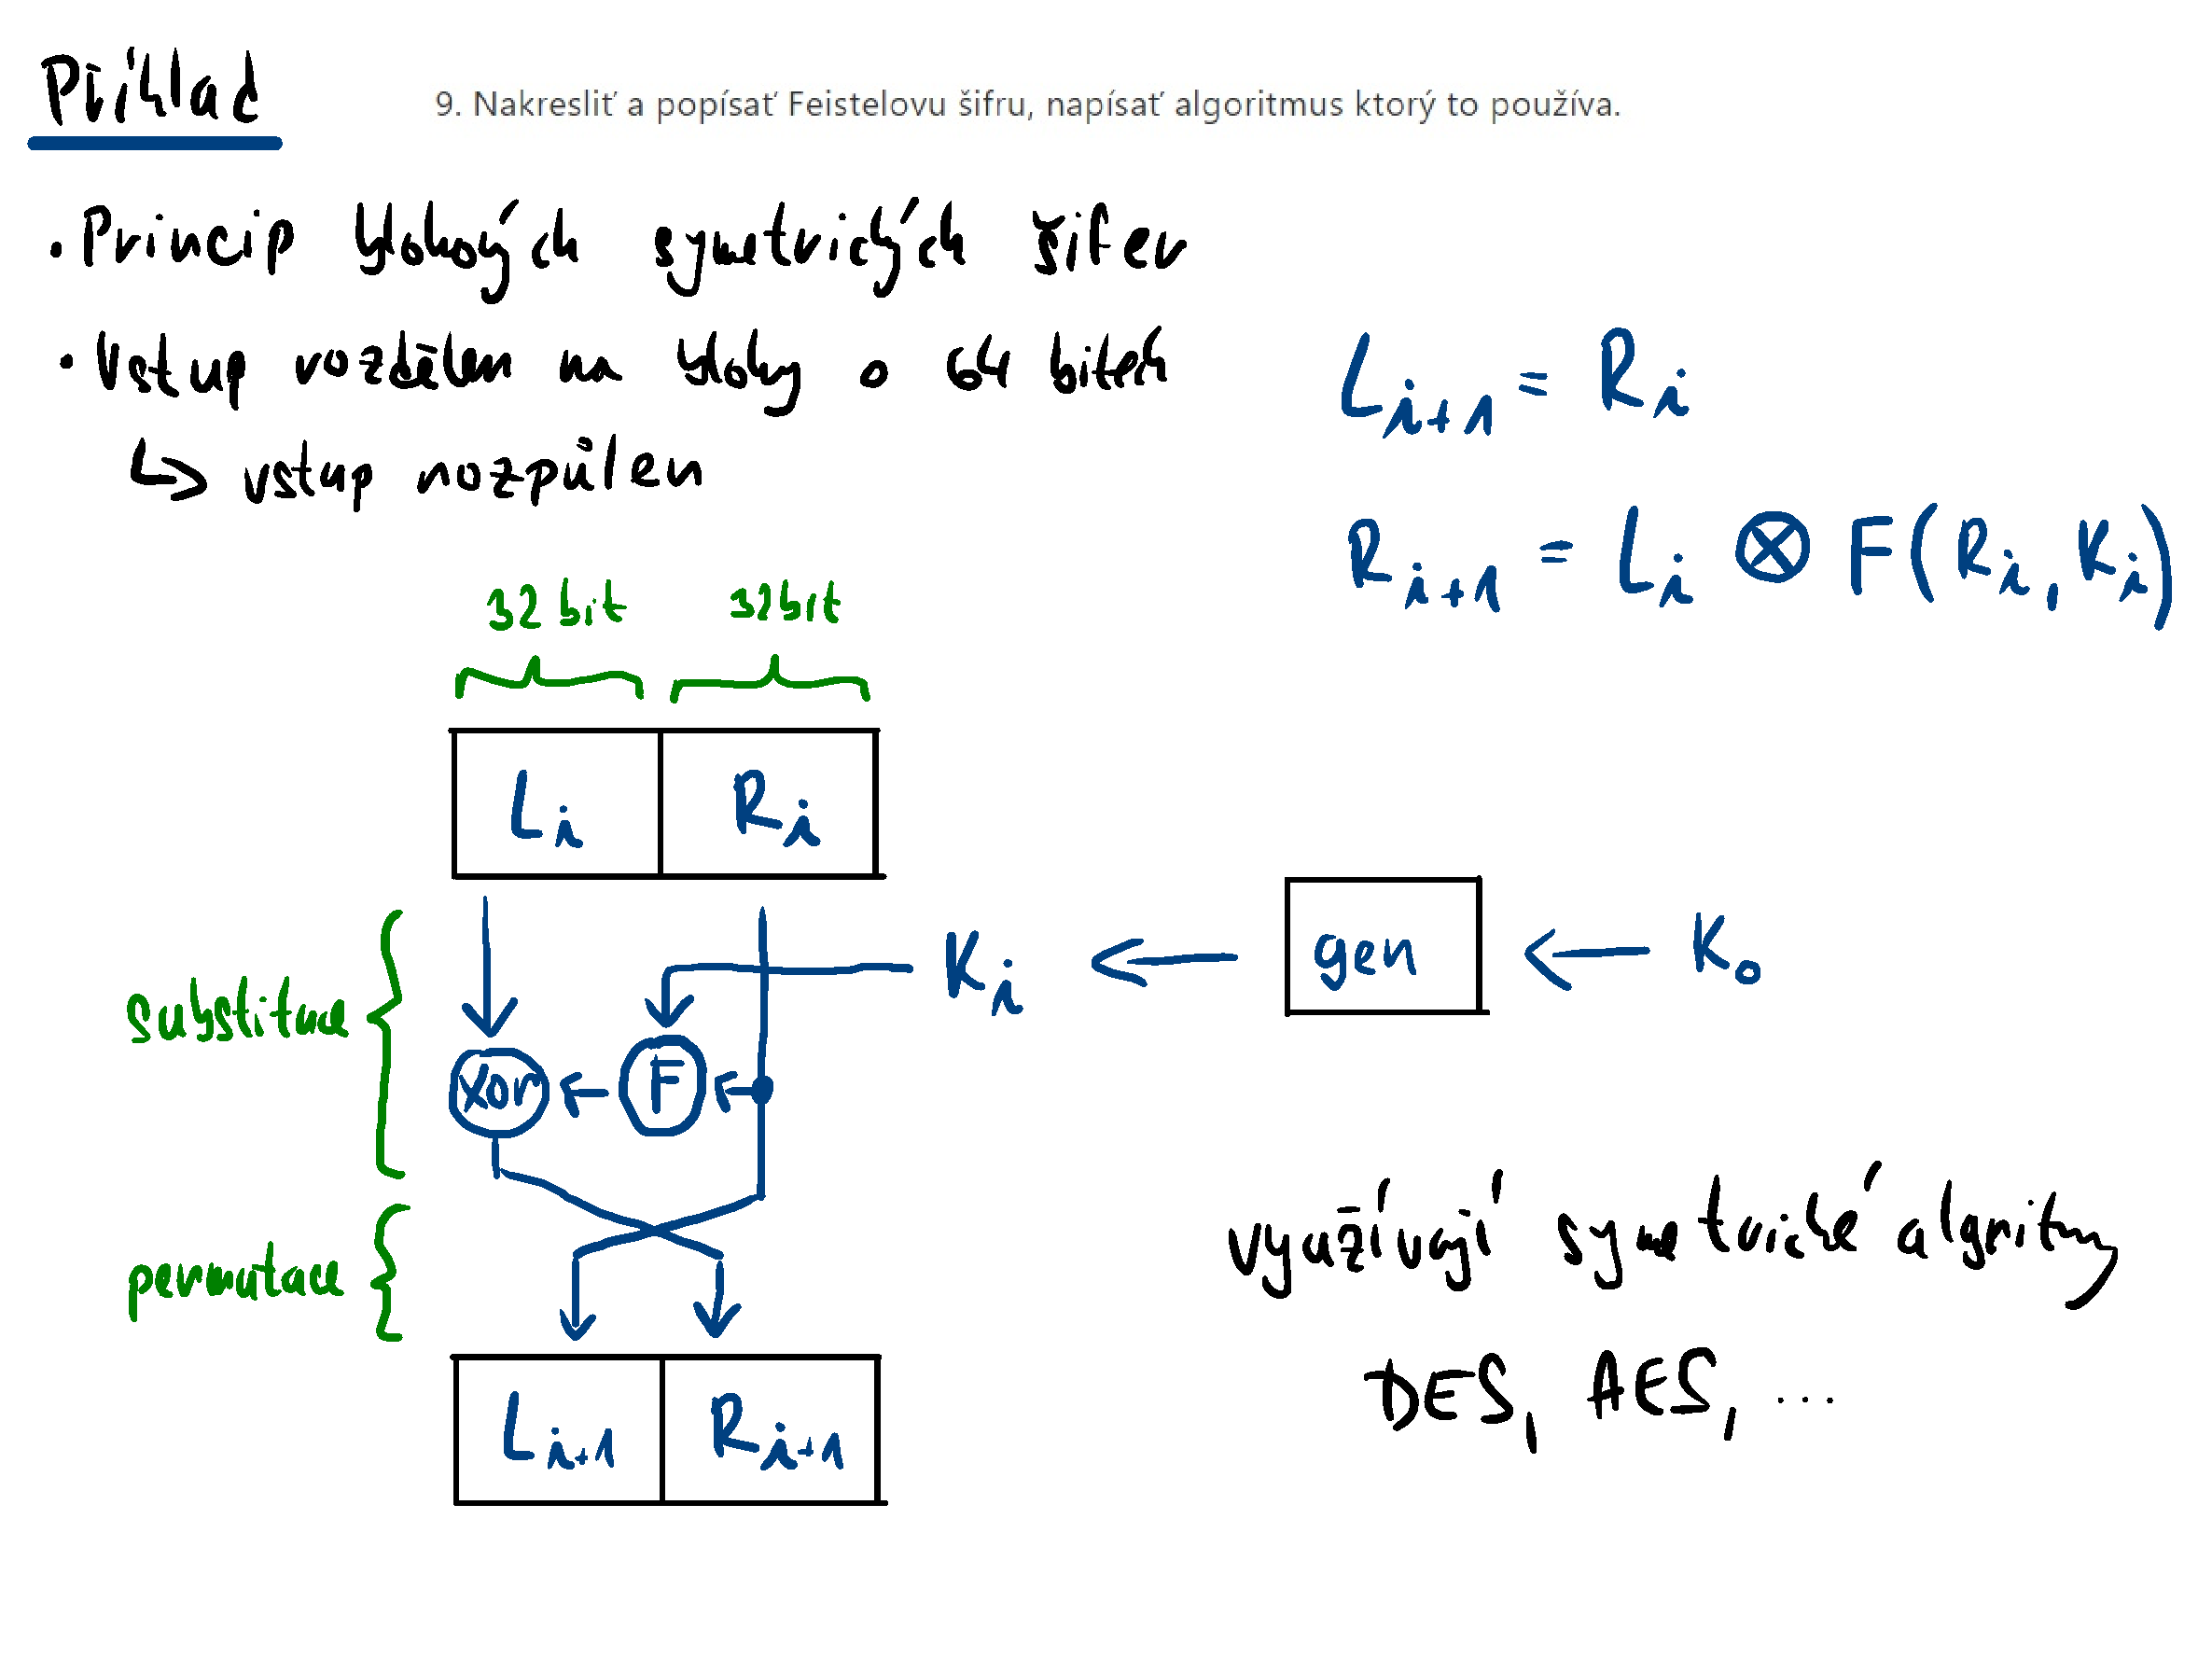
\includegraphics[width=1\linewidth]{feistel_example.pdf}
    \caption{Feistelova šifra -- příklad a rekapitulace.}
\end{figure}

\subsection{Data Encryption Standard (DES)}

DES byl první algoritmus s~veřejnou specifikací (\textit{security by design}). Využívá princip Feistelovy šifry -- 16 kol. Dodatečně přidává na začátek a konec permutaci navíc. Klíč je dlouhý 64b (resp. 56 významových bitů a 8 paritních).

\paragraph*{Slabiny} \begin{compactitem}
    \item 56 bitový klíč je příliš krátky a je možný útok silou.
    \item Rozdílná velikost bloku a klíče (zvláštnost).
    \item Existence slabých a poloslabých klíčů.
    \item Není jasné proč zrovna 16 iterací a zda je to dostatečné.
\end{compactitem}

\begin{figure}[H]
    \centering
    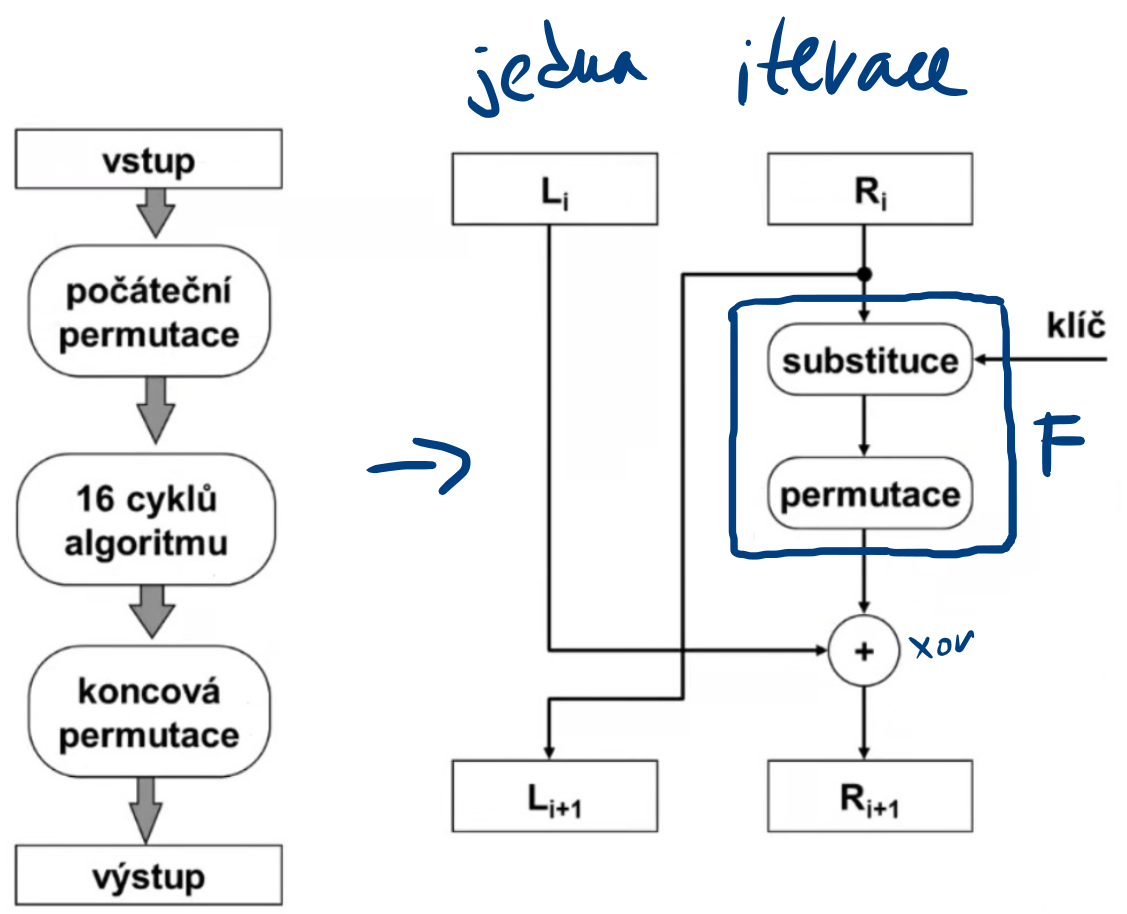
\includegraphics[width=0.75\linewidth]{des_schema.png}
    \caption{DES -- Schéma fungování algoritmu.}
\end{figure}

\begin{figure}[H]
    \centering
    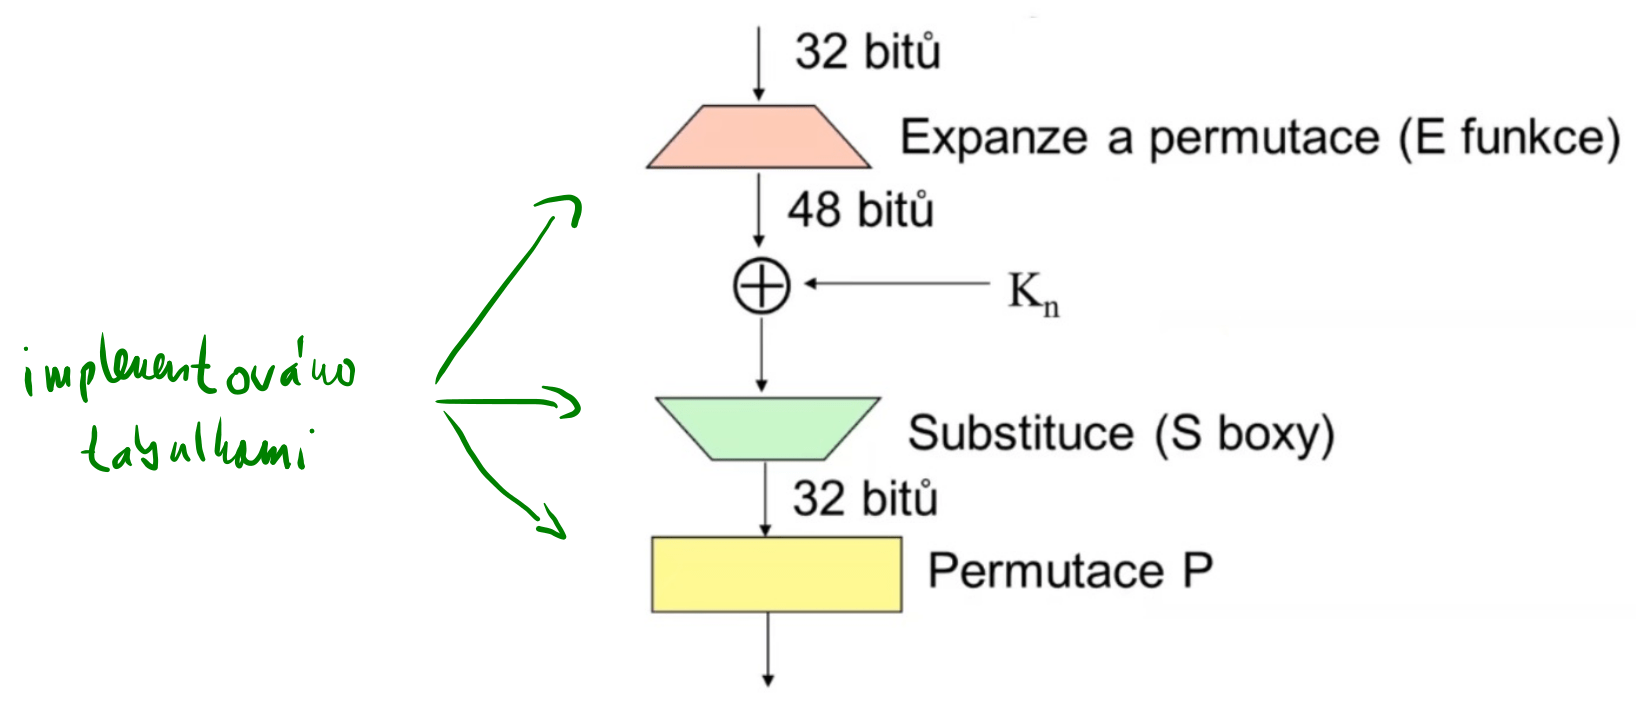
\includegraphics[width=1\linewidth]{des_f.png}
    \caption{DES -- funkce F.}
\end{figure}

\begin{figure}[H]
    \centering
    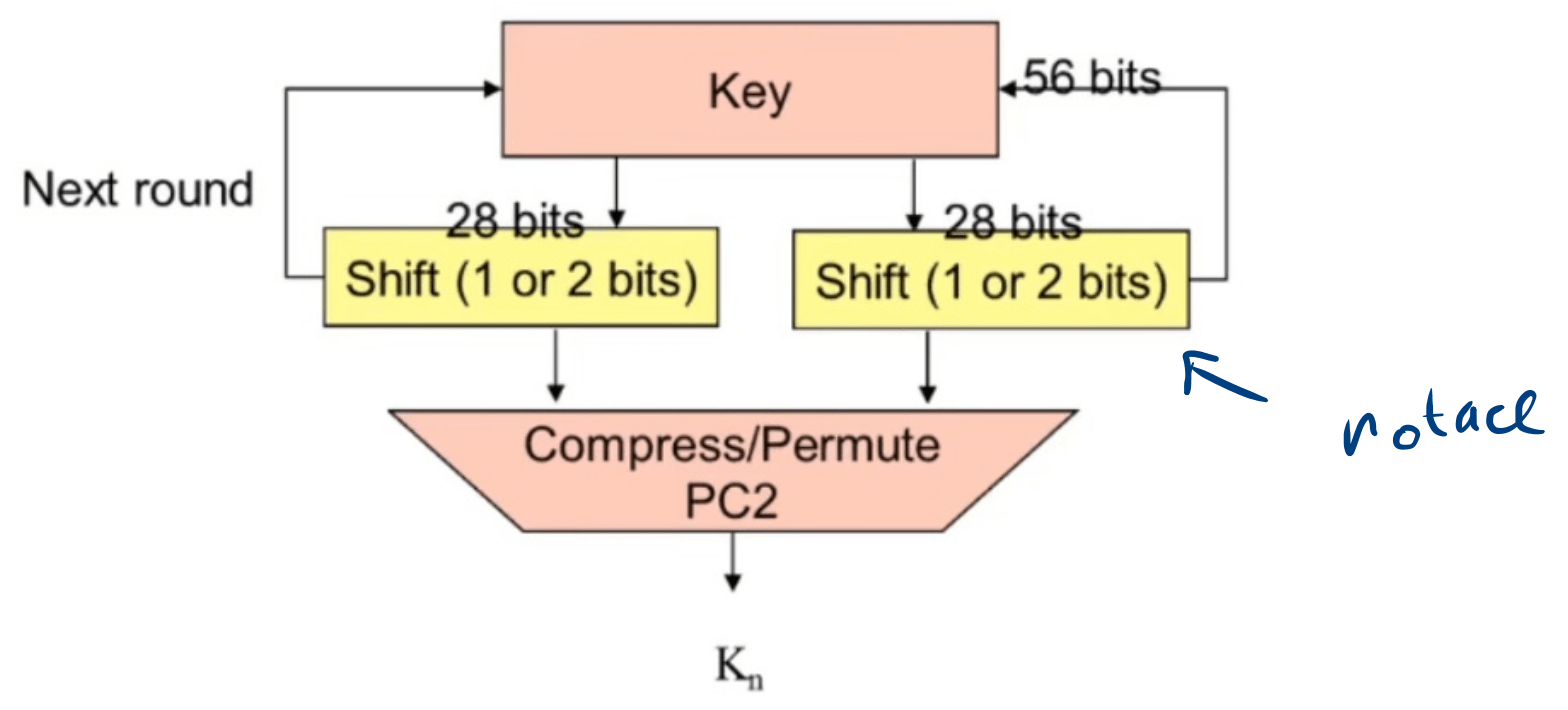
\includegraphics[width=1\linewidth]{des_keys.png}
    \caption{DES -- generování subklíčů.}
\end{figure}

\begin{figure}[H]
    \centering
    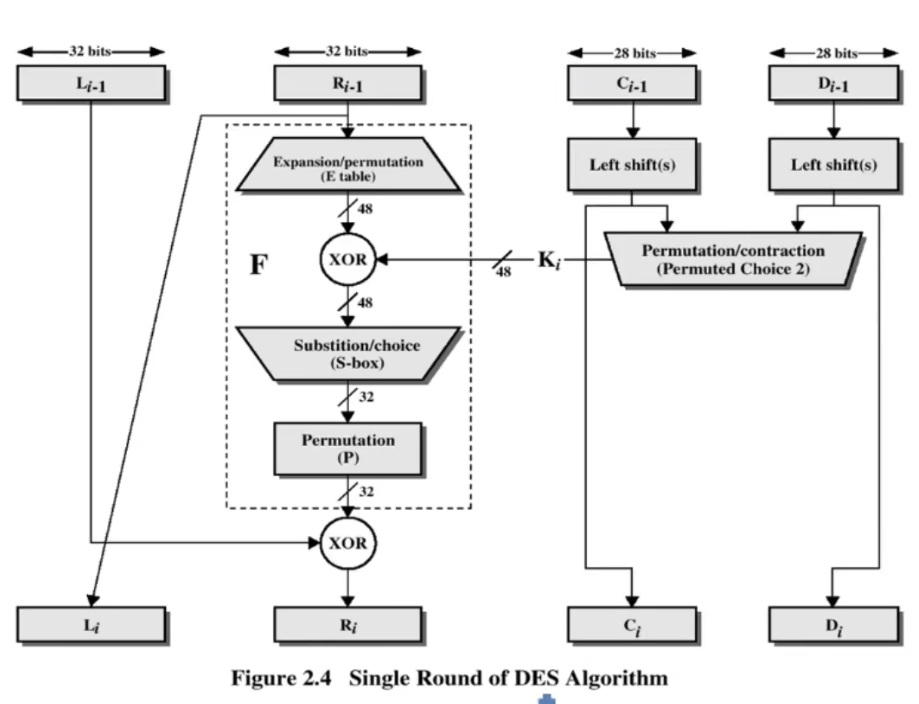
\includegraphics[width=1\linewidth]{des_single_round.png}
    \caption{DES -- jedno kolo algoritmu. \textit{Left shift} je ve skutečnosti bitová rotace.}
\end{figure}

\begin{figure}[H]
    \centering
    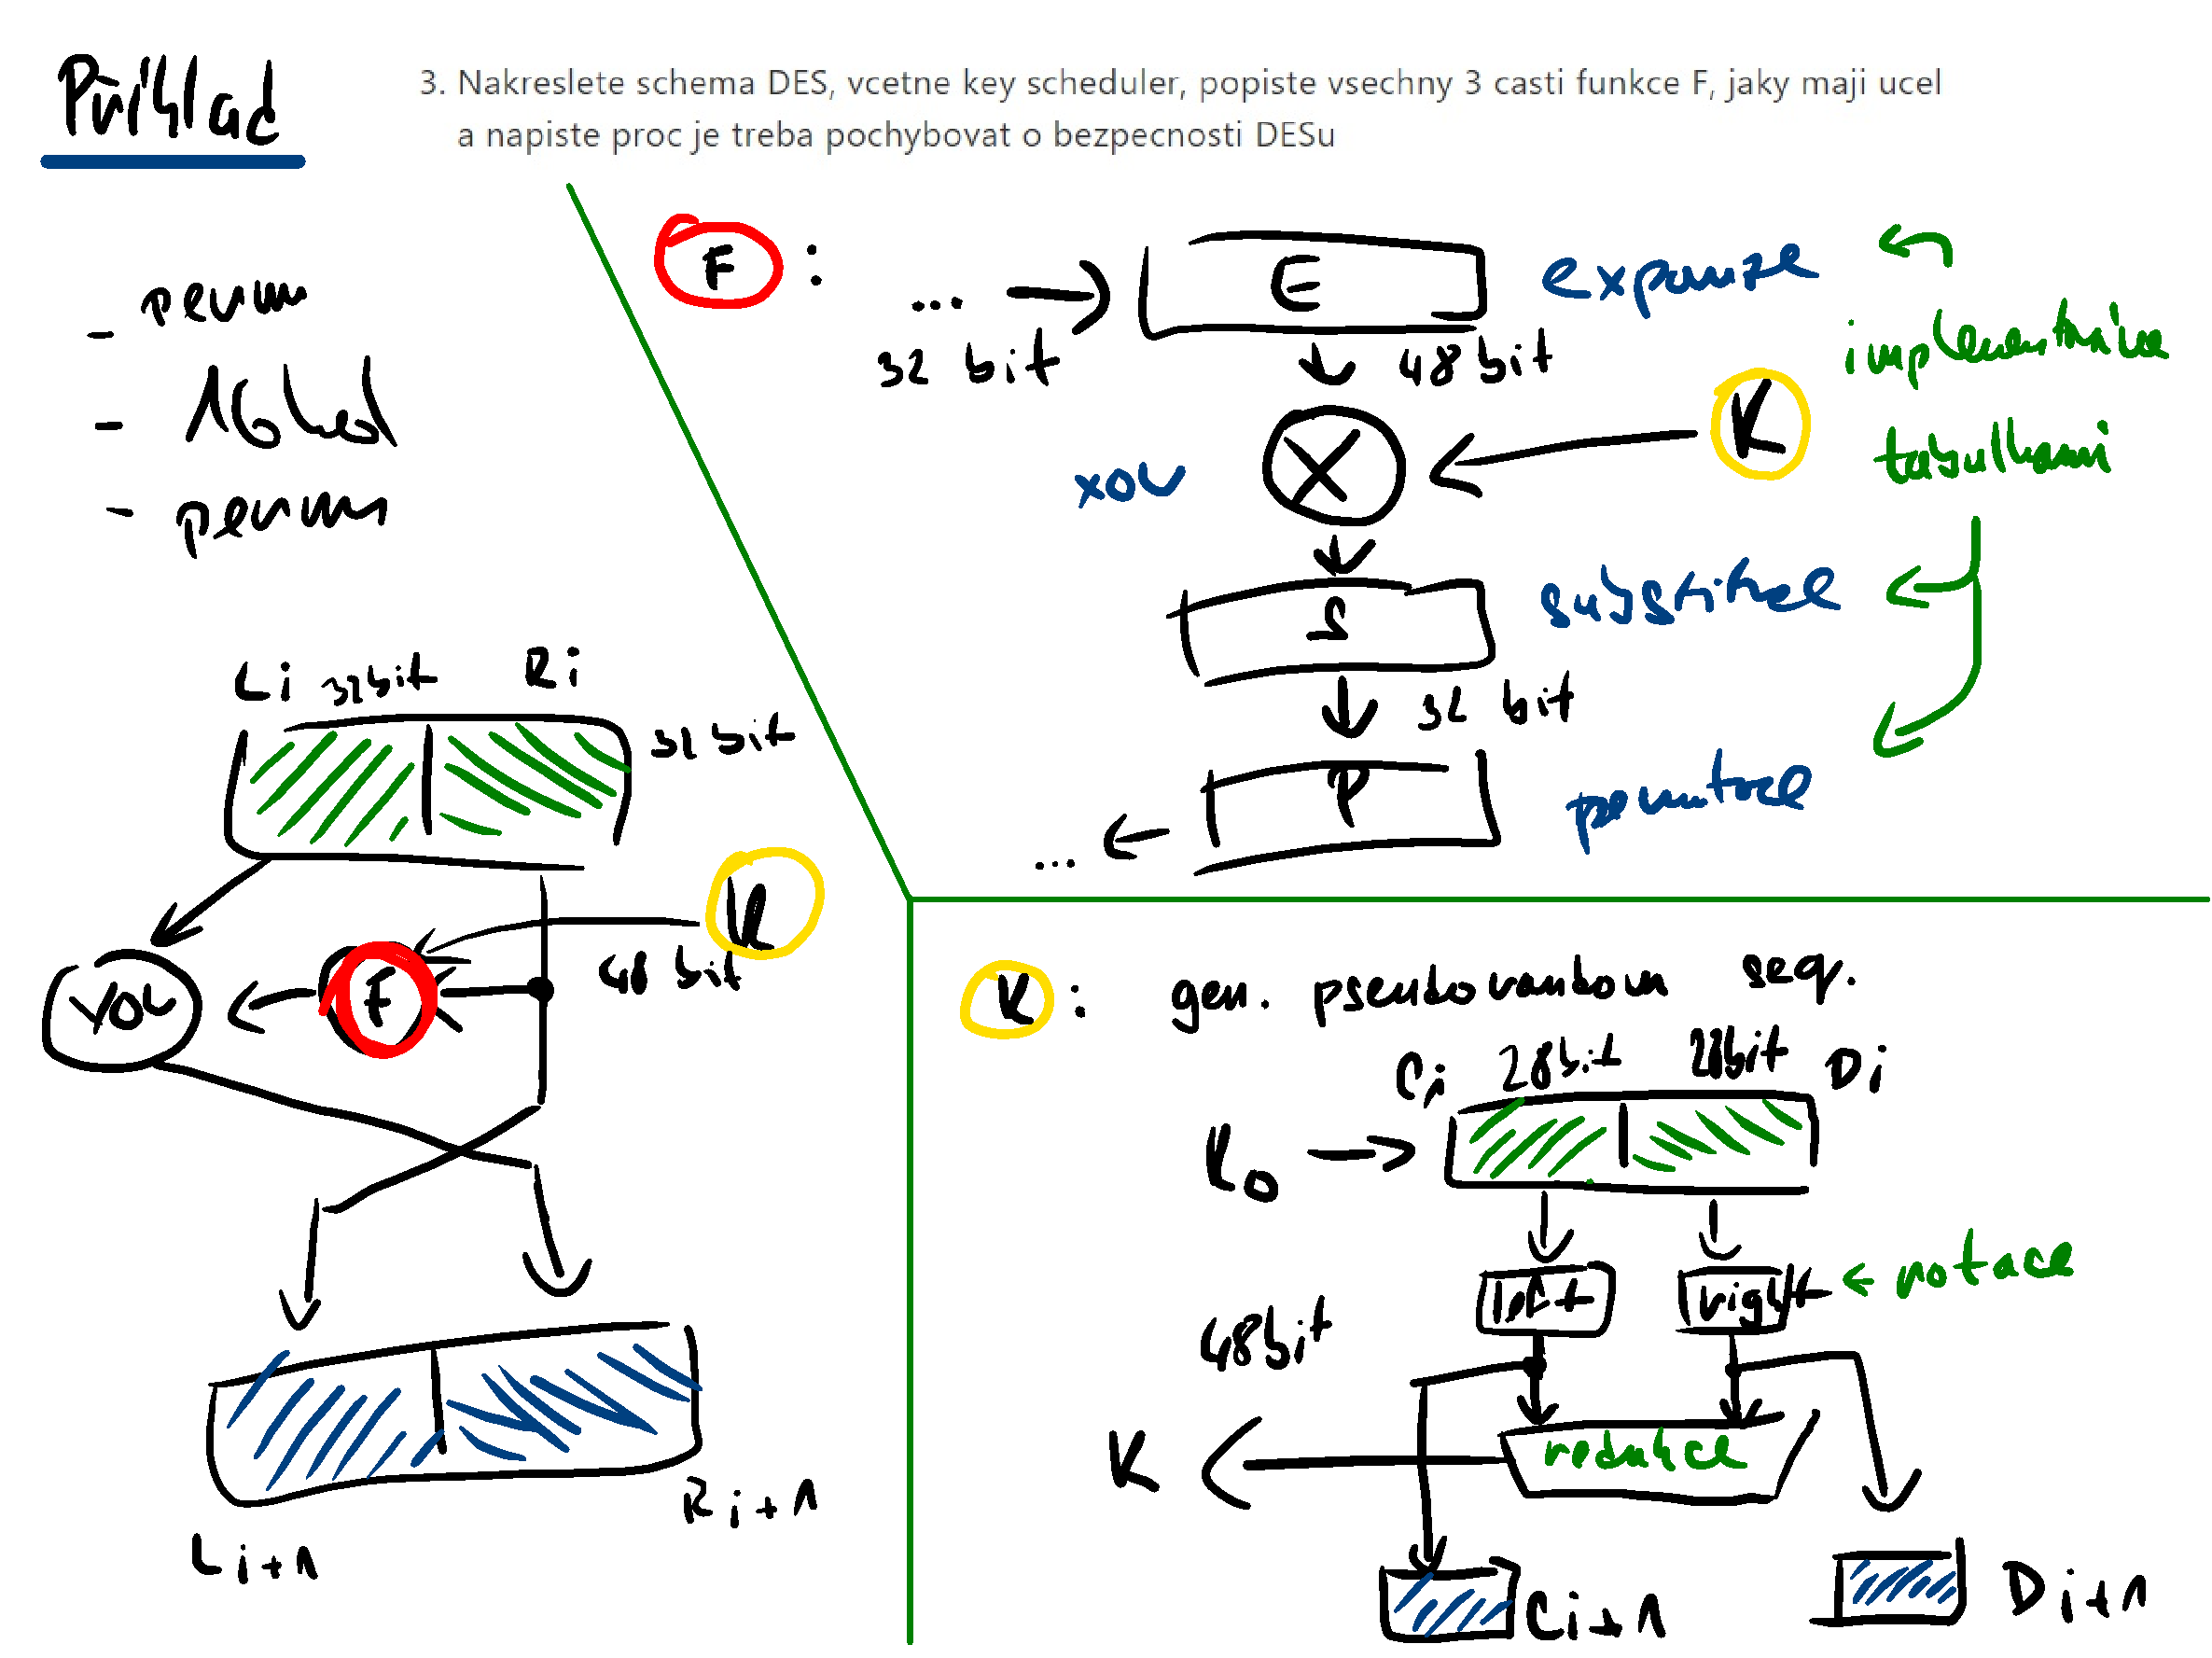
\includegraphics[width=1\linewidth]{des_example.pdf}
    \caption{DES -- příklad a rekapitulace.}
\end{figure}

%%%%%%%%%%%%%%%%%%%%%%%%%%%%%%%%%%%%%%%%%%%%%%%%%%%%%%%%%%%%%%%%%%%%%%%%%%%%%%%%

\section{Provozní režimy činnosti blokových šifer}

Jak použít blokové šifry abychom byli schopni šifrovat data delší než jeden blok?

\subsection{Electronic Code Book (ECB)}

ECB (\uv{kódová kniha}) je výchozí \textit{naivní} režim. Bloková šifra se při něm přímo aplikuje nezávisle na jednotlivé bloky, tedy při daném klíči odpovídá stejnému bloku otevřeného textu stejný blok šifrového textu. To má nežádoucí důsledky z~hlediska bezpečnosti, v~datech zůstane původní struktura, např. šifrovaný obrázek je rozpoznatelný.

\begin{figure}[H]
    \centering
    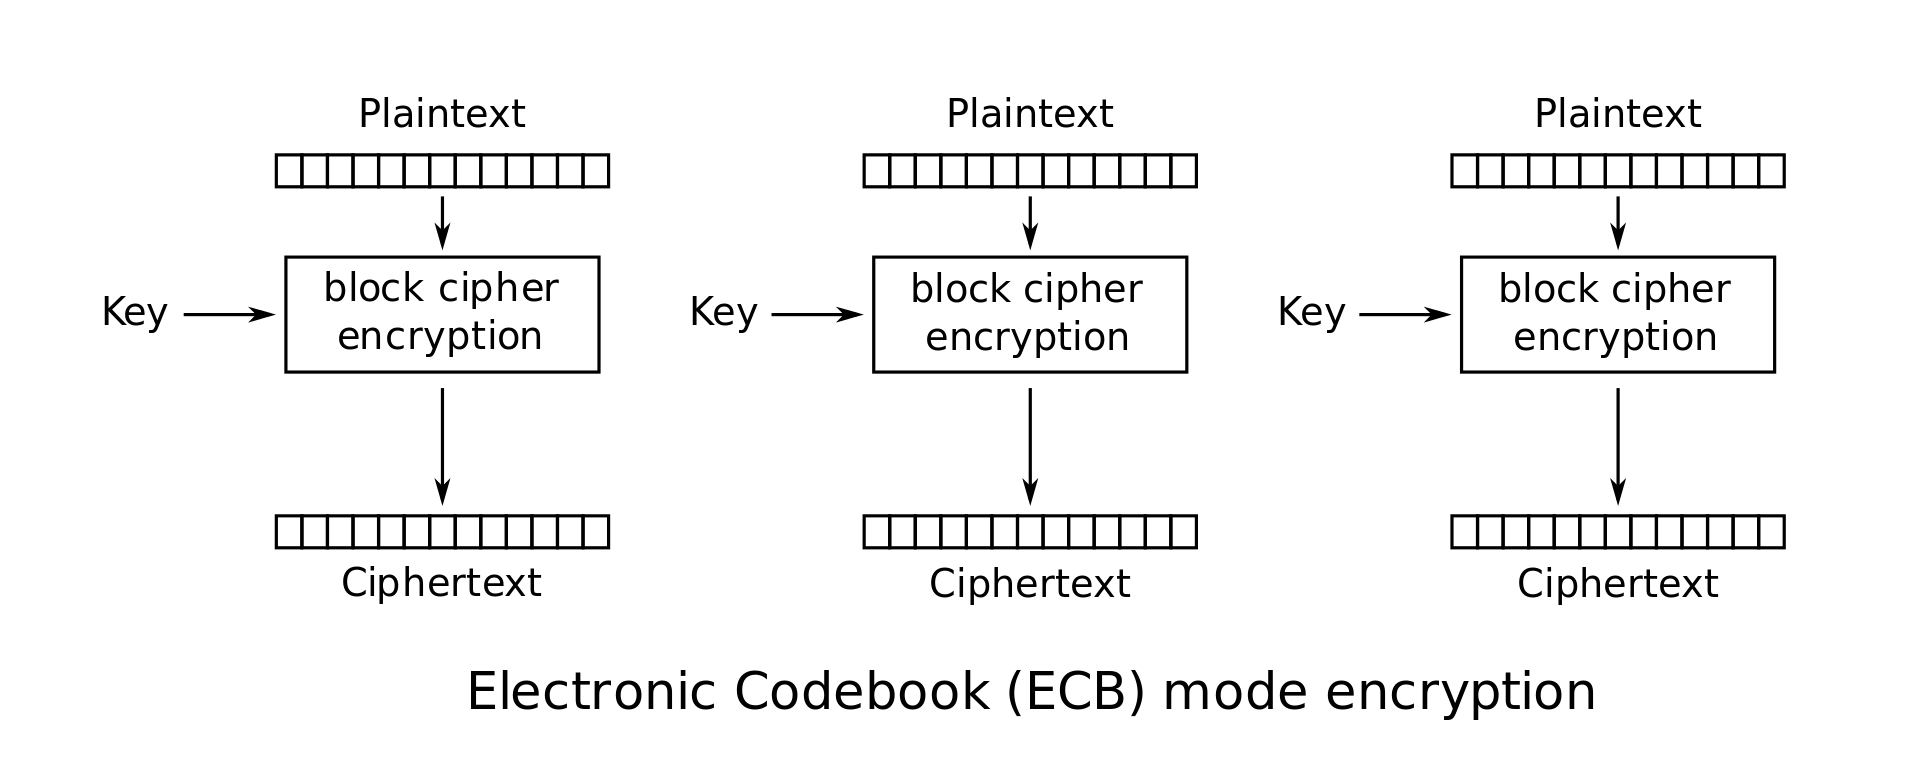
\includegraphics[width=1\linewidth]{rezim_ecb.png}
    \caption{Ukázka režimu ECB.}
\end{figure}

\subsection{Cipher Block Chaining (CBC)}

V~režimu CBC (\uv{řetězení šifrových bloků}) je každý blok před šifrováním xorován zašifrovaným předchozím blokem a první blok je xorován inicializačním vektorem. Tento režim je široce používán. Nevýhody plynou ze zřetězené závislosti (šifrovaný blok závisí na všech předcházejících): Šifrování nelze paralelizovat a při poškození šifrového bloku nelze dešifrovat ani blok přímo následující. Dešifrování paralelizovat lze.

\begin{equation}
\begin{aligned}
C_i &= E_K (P_i \oplus C_{i-1}) \\
P_i &= D_K(C_i) \oplus C_{i-1} \\
C_0 &= IV
\end{aligned}
\end{equation}

\begin{figure}[H]
    \centering
    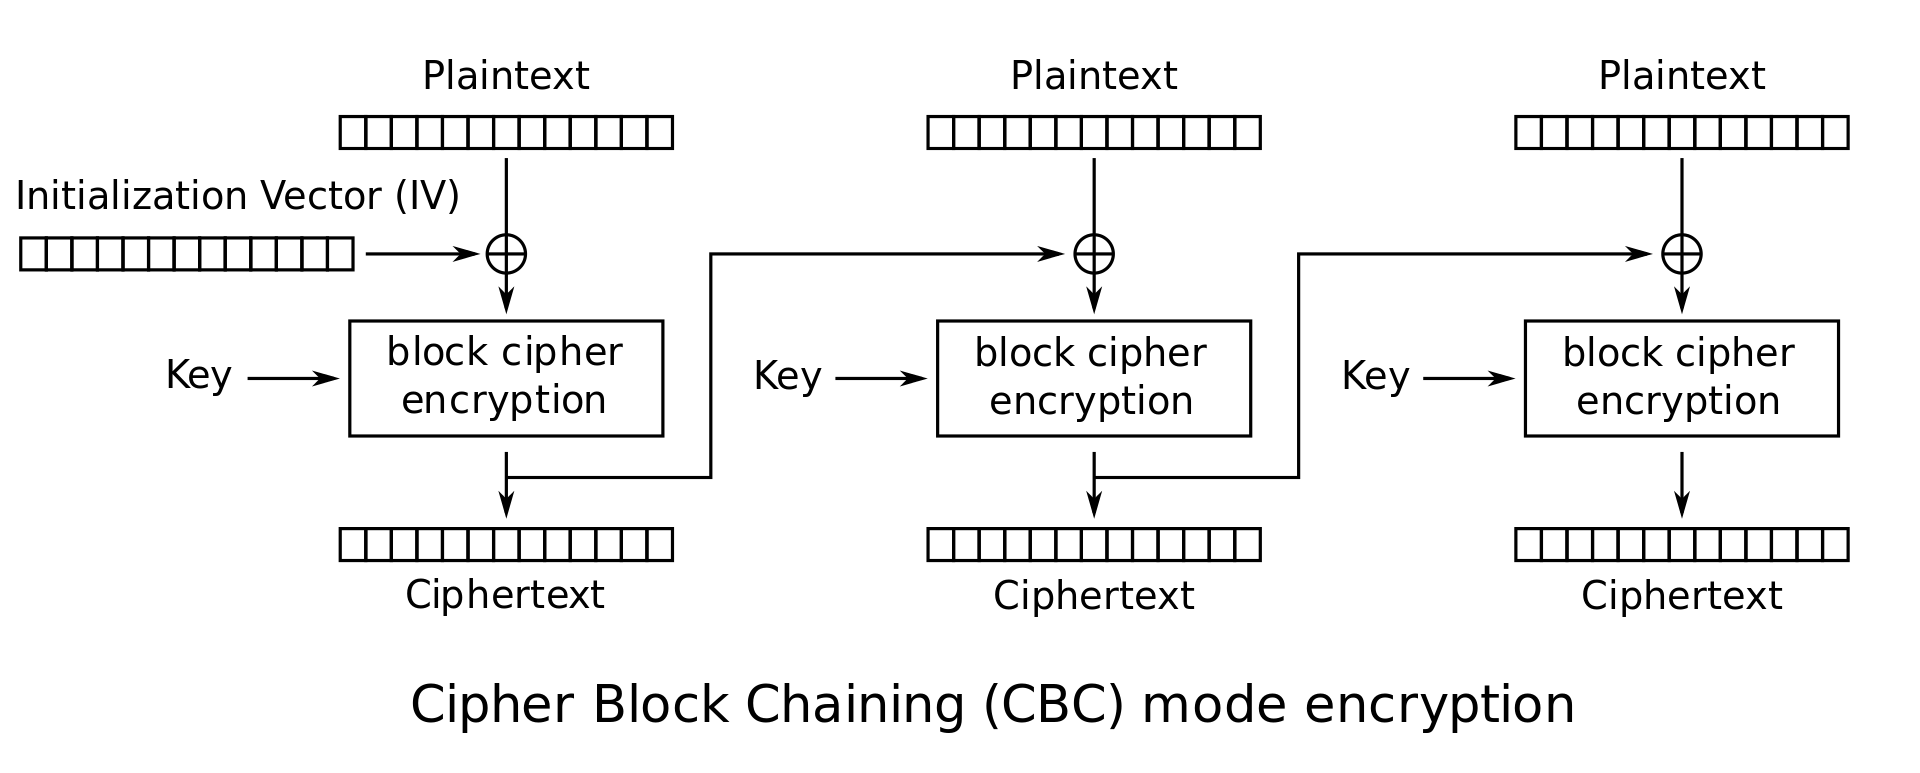
\includegraphics[width=1\linewidth]{rezim_cbc.png}
    \caption{Ukázka režimu CBC.}
\end{figure}

\subsection{Cipher Feedback (CFB)}

Režim CFB (\textit{šifrová zpětná vazba}) se liší oproti CBC v~prohození pořadí operací xor a šifrování -- nejprve se zašifruje předchozí šifrovaný blok (resp. inicializační vektor) a výsledek se xoruje s~otevřeným blokem. Toto prohození má významné implementační dopady: díky symetrii operace XOR vypadá dešifrovací funkce obdobně jako šifrovací. Šifruje pomaleji než CBC. Vstup není nutné zarovnávat. Plynou stejné nevýhody jako pro CBC.

\begin{equation}
\begin{aligned}
C_i &= E_K (C_{i-1}) \oplus P_i \\
P_i &= E_K (C_{i-1}) \oplus C_i \\
C_0 &= IV
\end{aligned}
\end{equation}

\begin{figure}[H]
    \centering
    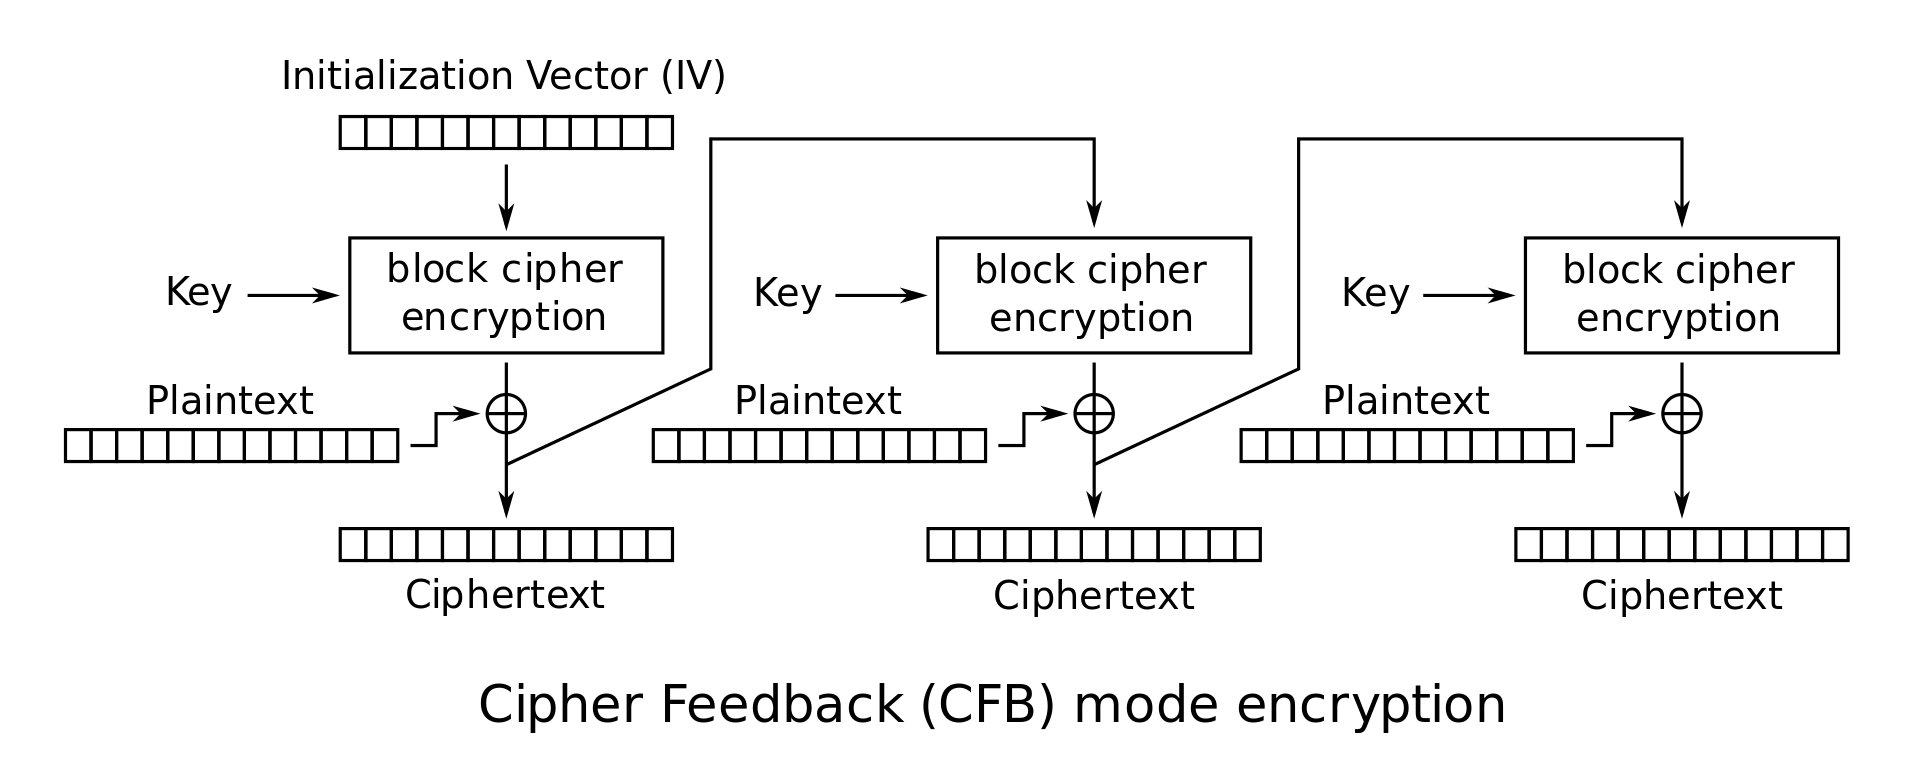
\includegraphics[width=1\linewidth]{rezim_cfb.png}
    \caption{Ukázka režimu CFB.}
\end{figure}

\subsection{Output Feedback (OFB)}

Režim OFB (\textit{výstupní zpětná vazba}) se liší od CFB pouze v~tom, kde bere zpětnou vazbu. Šifrování probíhá pouhým xorováním otevřeného bloku s~heslem, které je v~každém kroku zašifrováno použitou blokovou šifrou. První blok hesla je získán zašifrováním inicializačního vektoru. Režim převádí blokovou šifru na synchronní proudovou šifru.

\paragraph*{Slabina} Celý blok encryption je pouze generátor pseudonáhdon posloupnosti (je nezávislá na otevřeném nebo šifrovaném textu). To umožňuje Known Plaintext Attack. Z~toho plyne, že jedním klíčem není bezpečné šifrovat více než jednu zprávu.

\begin{equation}
\begin{aligned}
C_i &= E_K (C_{i-1}) \\
P_i &= P_i \oplus C_i \\
C_0 &= IV
\end{aligned}
\end{equation}

\begin{figure}[H]
    \centering
    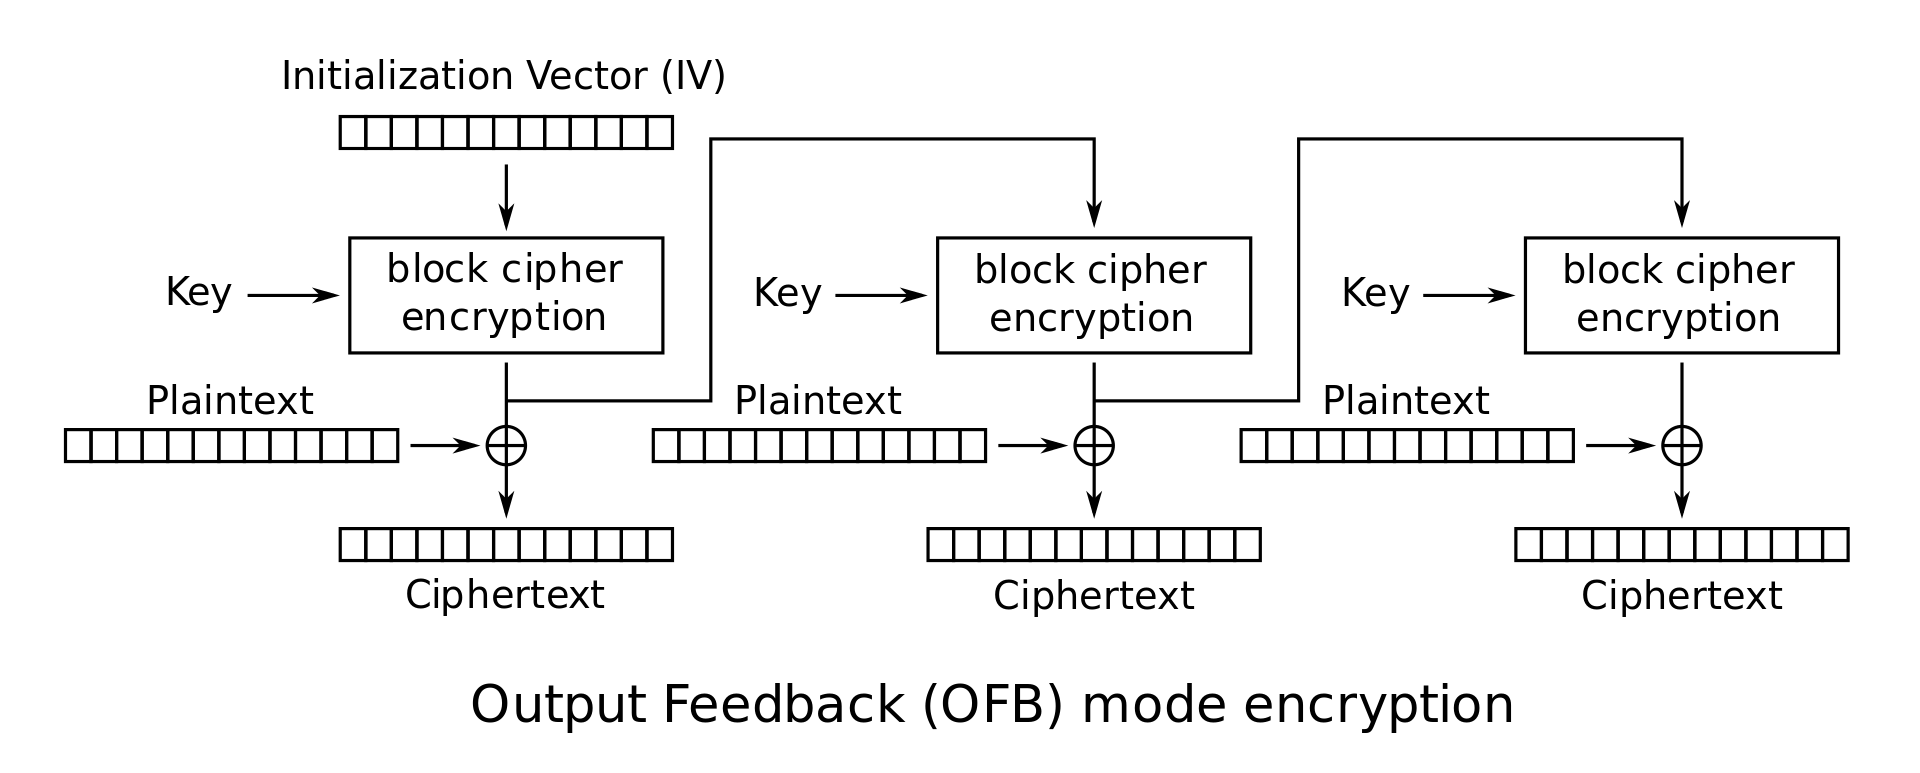
\includegraphics[width=1\linewidth]{rezim_ofb.png}
    \caption{Ukázka režimu OFB.}
\end{figure}

\subsection{Counter (CTR)}

Režim CTR (\uv{čítačový režim}) převádí stejně jako OFB blokovou šifru na synchronní proudovou. Heslo, se kterým se blok otevřeného textu xoruje, je však získáno zašifrováním čítače, který se každou iteraci zvětšuje o~pevně danou hodnotu, zpravidla o~1. Obsah čítače je opět před šifrováním nastaven inicializačním vektorem. Každý blok je šifrován nezávisle na ostatních, díky tomu je možné paralelizovat.

\begin{equation}
\begin{aligned}
CTR_i &= CTR_{i-1} + 1 \\
P_i &= P_i \oplus E_k(CTR_i) \\
CTR_0 &= IV
\end{aligned}
\end{equation}

\begin{figure}[H]
    \centering
    \includegraphics[width=1\linewidth]{rezim_ctr.png}
    \caption{Ukázka režimu CTR.}
\end{figure}

%%%%%%%%%%%%%%%%%%%%%%%%%%%%%%%%%%%%%%%%%%%%%%%%%%%%%%%%%%%%%%%%%%%%%%%%%%%%%%%%

\section{Proudové šifry}

Proudové šifry šifrují data jako \textit{proud} (stream), nejčastěji po jednotlivých bytech. Dešifrování vždy probíhá stejným způsobem. Proudové šifry jsou rychlejší než blokové šifry a pro implementaci potřebují jednodušší hardware.

\paragraph*{Problémy} \begin{compactitem}
    \item Nezajišťují samy o~sobě integritu.
    \item Na rozdíl od blokových šifer jsou náchylnější ke kryptoanalytickým útokům, pokud jsou nevhodně implementovány (počáteční stav nesmí být použit opakovaně)~--~\uv{problém s~inicializačním vektorem}.
\end{compactitem}

\begin{figure}[H]
    \centering
    \includegraphics[width=1\linewidth]{proudove.png}
    \caption{Princip proudových šifer.}
\end{figure}

\subsection{Rozdělení proudových šifer}

\paragraph*{Synchronní proudové šifry} Proud pseudonáhodných čísel \textit{key stream} je generován nezávisle na vstupním textu nebo zašifrované zprávě. Poté dochází ke kombinaci vygenerovaných čísel se vstupujícím textem (k~zakódování) nebo se šifrovaným textem (k~dekódování). Nejběžnější formou kombinace keystreamu a vstupního textu je použití operace XOR. Např.: Vernamova šifra, DES v~režimu OFB. Pokud se průběhu dešifrování něco ztratí, je konec.

\begin{figure}[H]
    \centering
    \includegraphics[width=0.5\linewidth]{proudova_synchronni.png}
    \caption{Princip synchronní proudové šifry.}
\end{figure}

\paragraph*{Samosynchronizující proudové šifry} Proud pseudonáhodných čísel \textit{key stream} závisí na pevném počtu předcházejících bytů šifrovaného (nebo otevřeného) textu. To znamená, že se šifra dokáže po chybě sama \textit{zotavit} (resynchronizovat)\footnote{Dnes se nesnážíme dešifrovat poškozená data, pokud nastane chyba v~přenosu, vyžádáme si data znovu.}. Např.: Vigenere Autokey, DES v~řežimu CFB.

\begin{figure}[H]
    \centering
    \includegraphics[width=0.75\linewidth]{proudova_samosynchronizujici.png}
    \caption{Princip samosynchronizující proudové šifry.}
\end{figure}

\subsection{Generátory PRNG}

Generátory PRNG (\textit{pseudo-random number generator}) generují pseudo-náhodnou pos\-loupnost (\textit{key stream}) z~malého klíče (\textit{seed}).

\paragraph*{Blokové šifry v~režimu OFB} Blokové šifry v~režimu OFB jsou pomalé.

\paragraph*{Linear Feedback Shift Registers (LSFR)} LFSR (posuvný registr s~lineární zpětnou vazbou) je posuvný registr, jehož výstup je lineárně závislý na jeho předchozích výstupech a stavu. Mějme \begin{compactitem}
    \item posuvný registr $R = (r_1, r_2, \dots, r_n)$,
    \item sekvenci zpětných vazeb $T = (t_1, t_2, \dots, t_n)$.
\end{compactitem}

\noindent Alternativně lze zapsat polynomem: $$
T(x) = x^n + x^{n-1} + \ldots + x + 1
$$

\begin{figure}[H]
    \centering
    \includegraphics[width=0.6\linewidth]{lfsr.png}
    \caption{Příklad LFSR.}
\end{figure}

\paragraph*{Geffe generátor} Geffe generátor (kombinovaný generátor) je využití 2 a více LFSR propojených multiplexorem.

\begin{figure}[H]
    \centering
    \includegraphics[width=0.75\linewidth]{geffe.png}
    \caption{Příklad Geffe generátoru.}
\end{figure}

\paragraph*{Stop and Go generátor} Stop and Go generátor je několik LSFR s~různým zdrojem hodin.

\begin{figure}[H]
    \centering
    \includegraphics[width=0.8\linewidth]{stop_and_go.png}
    \caption{Příklad Stop and Go generátoru.}
\end{figure}

\newpage

% 51
% VUT FIT MITAI
% MSZ 2021/2022
% Author: Vladimir Dusek
% Login: xdusek27

%%%%%%%%%%%%%%%%%%%%%%%%%%%%%%%%%%%%%%%%%%%%%%%%%%%%%%%%%%%%%%%%%%%%%%%%%%%%%%%%

% Path to figures
\graphicspath{{kry/asymetricka_kryptografie/figures}}

%%%%%%%%%%%%%%%%%%%%%%%%%%%%%%%%%%%%%%%%%%%%%%%%%%%%%%%%%%%%%%%%%%%%%%%%%%%%%%%%

\chapter{KRY -- Asymetrická kryptografie, vlastnosti, způsoby použití, poskytované bezpečnostní funkce, elektronický podpis a jeho vlastnosti, hybridní kryptografie, algoritmus RSA, generování klíčů, šifrování, dešifrování.}

% Todo:
% - Matematicke problemy by sly formulovat lepe a formalneji. To co tu mam, by lehce nemuselo stacit. Kouknout k materialum od Mateje Kastaka.
% Kongruence, multiplikativni inverze

%%%%%%%%%%%%%%%%%%%%%%%%%%%%%%%%%%%%%%%%%%%%%%%%%%%%%%%%%%%%%%%%%%%%%%%%%%%%%%%%

\section{Zdroje}

\begin{compactitem}
    \item Předmět: Kryptografie (KRY)
    \item Přednáška:
    \begin{compactitem}
        \item 6) Asymetrická kryptografie, vlastnosti, způsoby použití, poskytované bezpečnostní funkce.
        \item 7) Elektronický podpis a jeho vlastnosti, hybridní kryptografie.
        \item 8) Příklady asymetrických algoritmů, RSA.
    \end{compactitem}
    \item Záznam:
    \begin{compactitem}
        \item 2021-03-08
        \item 2021-03-22
    \end{compactitem}
\end{compactitem}

%%%%%%%%%%%%%%%%%%%%%%%%%%%%%%%%%%%%%%%%%%%%%%%%%%%%%%%%%%%%%%%%%%%%%%%%%%%%%%%%

\section{Úvod a kontext}

\textit{Viz. \uv{Úvod a kontext} v~předchozích otázkách z~tohoto předmětu.}

\paragraph*{Asymetrická kryptografie} \begin{compactitem}
    \item V~asymetrické kryptografii se používají páry klíčů (soukromý a veřejný). Soukromý je používán k~dešifrování, resp. vytvoření digitálního podpisu. Veřejný je používán k~šifrování, resp. ověření digitálního podpisu.
    \item Každý uživatel generuje svůj pár klíčů. Veřejný klíč je zveřejněn (znají ho všichni), sourkomý je držen v~tajnosti (zná ho pouze vlastník).
    \item Všechny asymetrické algoritmy jsou blokové.
    \item Asymetrické algoritmy jsou pomalejší než symetrické.
\end{compactitem}

\paragraph*{Způsoby použití} Asymetrická kryptografie lze využít k: \begin{compactitem}
    \item šifrování,
    \item digitálnímu podepisování,
    \item pro výměnu symetrického klíče (\textit{key exchange}).
\end{compactitem}

\paragraph*{Vlastnosti} Vlastnosti symetrické a asymetrické kryptografie\footnote{Otazníky -- částečně, za předpokladů, \dots}.
\begin{table}[H]
\begin{tabular}{lllll}
& Důvěrnost & Autentizace & Integrita & Nepopiratelnost \\
Symetrická & ano & ? & ? & ne \\
Asymetrická - šifrování & ano & ? & ? & ne \\
Asymetrická - podepisování & ne & ano & ano & ano \\
Asymetrická - kombinace & ano & ano & ano & ano
\end{tabular}
\end{table}

\bigskip\noindent\begin{minipage}{\linewidth}
\begin{lstlisting}[language=Python, caption={Kombinace klíčů obou stran u~asymetrický kryptografie. Pořadí operací může být i opačné.}]
# Odesilatel (A):
msg = encrypt(msg, SK_A) # necht msg je zprava k odeslani
msg = encrypt(msg, PK_B)
send(msg_2)

# Prijemce (B):
msg = receive()
msg = decrypt(msg, SK_B)
msg = decrypt(msg, PK_A)
\end{lstlisting}
\end{minipage}

\paragraph*{Digitální podpis} Vytvoření digitálního podpisu konkrétních dat pomocí soukromého klíče podepisatele. Každý kdo zná veřejný klíč podepisatele, může pravost podpisu ověřit. Digitální podpis zajišťuje autentizaci, itegritu a nepopiratelnost.

\paragraph*{Algoritmy} Algoritmy asymetrické kryptografie se nedají \textit{vymyslet}, musí se objevit. Jsou založeny na těžkých matematických problémech. \begin{compactitem}
    \item Problém batohu (\textit{knapsack problem}) -- MH (Merkle-Hellman)
    \item Faktorizace čísel -- RSA (Rivest-Shamir-Adleman)
    \item Diskrétní logaritmus -- DSA (Digital Signature Algorithm), DH (Diffie-Hellman)
    \item Eliptické křivky -- ECDSA, ECDH
\end{compactitem}

\paragraph*{Problém batohu} Problém batohu je NP-úplný problém kombinatorické optimalizace. Nechť ${x_1, x_2, \dots, x_n}$ je množina objektů, každý objekt má svoji cenu $v_i$ a svoji hmotnost $w_i$, dále mějme batoh, který má kapacitu $W$. Cílem je vybrat takovou množinu objektů, jejichž hmotnost je menší nebo rovna $W$ a má nejvyšší možnou cenu\footnote{Problém má více obdobných variant.}. Formálně chceme maximalizovat sumu $$ \sum_{i=1}^n v_i \cdot x_i $$, při splnění $$ \sum_{i=1}^n w_i \cdot x_i \leq W $$, kde $x_i \in {x_1, x_2, \dots, x_n}$.

\paragraph*{Faktorizace čísel} Faktorizace čísel označuje problém rozložení čísla na součin menších čísel, v~nejčastější podobě pak rozklad celého čísla na součin prvočísel.

\paragraph*{Diskrétní logaritmus} Nechť $p, g, k, Y$ jsou přirozená čísla, pro něž platí $Y \equiv g^{k} \; \text{mod} \; p$. Potom každé číslo $k$ odpovídající uvedené rovnici nazveme diskrétní logaritmus o~základu $g$ z~$Y$ vzhledem k~modulu $p$. Tato definice nedefinuje číslo $k$ jednoznačně, proto se někdy upravuje tak, že ze všech možných diskrétních logaritmů ve smyslu předchozí definice se vybere ten nejmenší.

\paragraph*{Eliptické křivky} Jedná se o~matematický aparát, na kterém aplikujeme různé algoritmy (DSA, DH).

%%%%%%%%%%%%%%%%%%%%%%%%%%%%%%%%%%%%%%%%%%%%%%%%%%%%%%%%%%%%%%%%%%%%%%%%%%%%%%%%

\section{Hybridní kryptografie}

Hybridní kryptografie je kombinace symetrické a asymetrické kryptografie, ve které jsou využity přednosti obou (symetrická -- rychlá, ale potřeba stejný klíč; asymetrická -- pomalá, ale dva klíče). Asymetrická je využita pro bezpečné zaslání symetrického klíče.

\begin{figure}[H]
    \centering
    \includegraphics[width=1\linewidth]{hybrid_utajeni.pdf}
    \caption{Schéma utajení hybridní kryptografie.}
\end{figure}

\begin{figure}[H]
    \centering
    \includegraphics[width=1\linewidth]{hybrid_podpis.pdf}
    \caption{Schéma digitálního podpisu hybridní kryptografie.}
\end{figure}

%%%%%%%%%%%%%%%%%%%%%%%%%%%%%%%%%%%%%%%%%%%%%%%%%%%%%%%%%%%%%%%%%%%%%%%%%%%%%%%%

\section{RSA}

Algoritmus RSA (Rivest-Shamir-Adleman) lze použít jak pro šifrování dat pro digitální podepisování. Je založen na problému faktorizace velkých čísel.

\paragraph*{Klíče} Klíče se skládají z: \begin{compactitem}
    \item $p, q$ -- dvě náhodná soukromá prvočísla,
    \item $n$ -- veřejný modul ($n = p \cdot q$),
    \item $e$ -- veřejný exponent ($e < \Phi(n) \; \land \; GCD(\Phi(n), e) = 1$), typicky $3$ nebo $2^{16}+1$\footnote{$GCD$~--~největší společný dělitel},
    \item $d$ -- soukromý exponent,
    \item musí platit vztah: $e \cdot d \; \text{mod} \; \Phi(n) = 1$.
\end{compactitem}

\noindent Veřejný klíč $PK = (n, e)$, soukromý klíč $SK = (n, d)$.

\paragraph*{Postup generování} Postup generování klíčů: \begin{compactenum}
    \item vygenerovat prvočísla $p$ a $q$,
    \item spočítat modul $n = p \cdot q$,
    \item spočítat $\Phi(n) = (p-1) \cdot (q-1)$,
    \item zvolit veřejný exponent $e < \Phi(n) \; \land \;GCD(\Phi(n), e) = 1$,
    \item spočítat soukromý exponent $d$ tak, že platí $e \cdot d \; \text{mod} \; \Phi(n) = 1$.
\end{compactenum}

\paragraph*{Šifrování a dešifrování} Mějme zprávu $m$ reprezentovanou jako celé číslo a zašifrovanou zprávu $c$ reprezentovanou také jako celé číslo. Digitální podpis se vytváří stejným způsobem, pouze se prohodí exponenty.

\begin{equation}
    c = m^e \; \text{mod} \; n
\end{equation}

\begin{equation}
    m = c^d \; \text{mod} \; n
\end{equation}

\paragraph*{Útoky a slabiny} Pokud útočník rozloží číslo $n$ na činitele $p$ a $q$, tak může dopočítat soukromý klíč. Pokud útočník uhádně hodnotu $(p-1) \cdot (q-1)$, tak může dopočítat soukromý klíč. Šifrování malých čísel je zranitelné, proto se používá \uv{předzpracování}~--~zarovnání na $X$ bitů (2048).

\begin{figure}[H]
    \centering
    \includegraphics[width=1\linewidth]{rsa_example.pdf}
    \caption{Příklad RSA.}
\end{figure}

\newpage

% 52
% VUT FIT MITAI
% MSZ 2021/2022
% Author: Vladimir Dusek
% Login: xdusek27

%%%%%%%%%%%%%%%%%%%%%%%%%%%%%%%%%%%%%%%%%%%%%%%%%%%%%%%%%%%%%%%%%%%%%%%%%%%%%%%%

% Path to figures
\graphicspath{{kry/hasovaci_funkce/figures}}

%%%%%%%%%%%%%%%%%%%%%%%%%%%%%%%%%%%%%%%%%%%%%%%%%%%%%%%%%%%%%%%%%%%%%%%%%%%%%%%%

\chapter{KRY -- Hašovací funkce, klíčovaný haš a MAC a jejich použití a vlastnosti.}

%%%%%%%%%%%%%%%%%%%%%%%%%%%%%%%%%%%%%%%%%%%%%%%%%%%%%%%%%%%%%%%%%%%%%%%%%%%%%%%%

\section{Zdroje}

\begin{compactitem}
    \item Předmět: Kryptografie (KRY)
    \item Přednáška:
    \begin{compactitem}
        \item \path{KRY04_Asym_MNG.pdf}
    \end{compactitem}
    \item Záznam:
    \begin{compactitem}
        \item 2021-03-22
    \end{compactitem}
\end{compactitem}

%%%%%%%%%%%%%%%%%%%%%%%%%%%%%%%%%%%%%%%%%%%%%%%%%%%%%%%%%%%%%%%%%%%%%%%%%%%%%%%%

\section{Úvod a kontext}

\textit{Viz. \uv{Úvod a kontext} v~předchozích otázkách z~tohoto předmětu.}

\paragraph*{Hashovací funkce} Hashovací funkce je funkce (resp. algoritmus) pro převod vstupních dat do (relativně) malého čísla. Výstup hashovací funkce se označuje otisk, \textit{fingerprint}, \textit{digest} či \textit{hash}. Jsou jednosměrné a odolné proti kolizím (viz vlastnosti).

\paragraph*{Obecné vlastnosti} Hashovací funkce by měla: \begin{compactitem}
    \item Být aplikovatelná na argument o~libovolné velikosti.
    \item Mít výstyp konstantní délky.
    \item Dokázat spočítat výstup rychle.
\end{compactitem}

\paragraph*{Neklíčované hashovací funkce} Hashovací funkce má pouze jeden argument~--~data. Např. MD2, MD4, MD5, SHS, SHA1, SHA2, SHA3. $$f(data) \rightarrow hash$$

\paragraph*{Klíčované hashovací funkce} Hashovací funkce má dva argumenty~--~data a klíč. Také se jim někdy říká MAC (\textit{message authentication code}). $$f(data, key) \rightarrow hash$$

\paragraph*{Lavinový efekt} Lavinový efekt \textit{Avalanche Effect} je žádoucí vlastností kryptografických algoritmů, typicky blokových šifer a kryptografických hašovacích funkcí, kdy se při nepatrné změně vstupu (například převrácení jednoho bitu) výrazně změní výstup (např. převrátí se polovina výstupních bitů). V případě kvalitních blokových šifer by taková malá změna klíče nebo otevřeného textu měla způsobit drastickou změnu šifrového textu.

%%%%%%%%%%%%%%%%%%%%%%%%%%%%%%%%%%%%%%%%%%%%%%%%%%%%%%%%%%%%%%%%%%%%%%%%%%%%%%%%

\section{Kryptografická odolnost hashovacích funkcí}

\paragraph*{Vlastnosti z~hlediska odolnosti} Hashovací funkce by z~hlediska kryptografické odolnosti měly splňovat: \begin{compactitem}
    \item \textit{First preimage resistance}~--~Pro konkrétní $y$ je výpočetně nezvládnutelné najít takové $x$, aby platilo $h(x) = y$. Útočník má k~dispozici konkrétní hash, a snaží se pro něho nalézt zprávu.
    \item \textit{Second preimage resistance}~--~Pro konkrétní $x$ je výpočetně nezvládnutelné najít takové $x'$, aby platilo $h(x) = h(x')$. Útočník má k~dispozici konkrétní zprávu (nemůže si ji zvolit), ke které se snaží nalézt jinou zprávu, která bude mít stejný hash.
    \item \textit{Collision resistance}~--~Je výpočetně nezvládnutelné najít libovolnou dvojici $x, x'$ takovou, aby platilo $x \neq x'$ a $h(x) = h(x')$. Útočník si může zvolit libovolnou zprávu, ke které se snaží nalézt jinou zprávu, která bude mít stejný hash. Pokud platí \textit{collision resistance}, tak platí i \textit{second preimage resistance}.
\end{compactitem}

\paragraph*{Narozeninový problém} V~teorii pravděpodobnosti je narozeninový problém úloha vypočítat minimální početnost skupiny lidí, ve které je alespoň 50\% pravděpodobnost nalezení dvojice se stejným datem narození. Narozeninovým paradoxem je pak označována skutečnost, že tento počet (23) je mnohem menší než intuitivní odhad.
Výsledek je intuitivnější, když uvážíme, že porovnání narozenin bude provedeno mezi všemi možnými dvojicemi jedinců. Při počtu 23 jedinců je třeba uvažovat $(23 \cdot 22) / 2 = 253$ dvojic, což je více než polovina počtu dnů v~roce ($182,5$).

Jednodušší je nejprve spočítat jev opačný $\bar p(n)$, tedy pravděpodobnost, že všech $n$ narozenin je rozdílných. Pro $n > 365$ je $1$, jinak:
\begin{equation}
\begin{aligned}
\bar p(n) &= 1 \cdot \left(1-\frac{1}{365}\right) \cdot \left(1-\frac{2}{365}\right) \cdots \left(1-\frac{n-1}{365}\right) = \\
&=  \frac{365 \cdot 364 \cdots (365-n+1)}{365^n} = \\
&=  \frac{365!}{365^n (365-n)!}
\end{aligned}
\end{equation}

\begin{equation}
    p(n) = 1 - \bar p(n)
\end{equation}

\paragraph*{Narozeninový útok} Mějme hashovací funkci, která má $n$ bitový výstup (celkový počet možných hashů je $2^{n}$). Útočník vytvoří dokument \uv{přátelská dohoda} a přibližně $2^{n/2}$ sémanticky ekvivalentních verzí (úprava bílých znaků, úprava pořadí celků, jiné formulace, \dots). Podobně vytvoří dokument \uv{nepřátelská dohoda} a přibližně $2^{n/2}$ sémanticky ekvivalentních verzí. S~pravděpodobností $0,5$ existuje verze \uv{přátelské dohody} a \uv{nepřátelské dohody}, které mají stejný hash. Pokud takové verze existují, útočník dá oběti podepsat \uv{přátelskou dohodu} $\Rightarrow$ existuje validní podpis \uv{nepřátelské dohody}.

\paragraph*{Bezpečnostní cíle OWHF} Bezpečnostní cíle OWHF (\textit{one way hash function}). Některé protokoly nevyžadují bezkoliznost, proto má smysl řešit i tento případ. \begin{compactitem}
    \item Vyžadované vlastnosti: \textit{first preimage resistance} a \textit{second preimage resistance}
    \item Cíl útočníka: vytvořit \textit{first preimage} nebo \textit{second preimage} (oba úkoly jsou stejně těžké)
    \item Složitost: $O(2^n)$ ($n$ je počet bitů hashe)
    \item Požadovaná délka: $n \geq 80$
\end{compactitem}

\paragraph*{Bezpečnostní cíle CRHF} Bezpečnostní cíle CRHF (\textit{collision resistance hash function}). \begin{compactitem}
    \item Vyžadované vlastnosti: \textit{collision resistance}
    \item Cíl útočníka: vytvořit kolizi
    \item Složitost: $O(2^{n / 2})$ ($n$ je počet bitů hashe) (kvůli narozeninovému útoku)
    \item Požadovaná délka: $n \geq 160$
\end{compactitem}

\paragraph*{Bezpečnostní cíle MAC} Bezpečnostní cíle MAC (\textit{message authentication code}). \begin{compactitem}
    \item Vyžadované vlastnosti: \textit{computation resistance}, \textit{key non-recovery}
    \item Cíl útočníka (útočník si může vybrat): \begin{compactitem}
        \item Vytvořit nový hash, který bude odpovídat nové zprávě
        \item Nalézt klíč
    \end{compactitem}
    \item Složitost ($n$ je počet bitů hashe, $t$ je počet bitů klíče): \begin{compactitem}
        \item Vytvořit nový hash: $O(max(2^{-n}, 2^{-t}))$
        \item Nalézt klíč: $O(2^n)$
    \end{compactitem}
    \item Požadovaná délka: $n \geq 64 \; \land \; t \geq 64$
\end{compactitem}

%%%%%%%%%%%%%%%%%%%%%%%%%%%%%%%%%%%%%%%%%%%%%%%%%%%%%%%%%%%%%%%%%%%%%%%%%%%%%%%%

\section{Hashovací funkce neklíčované}

Nejčastější způsoby sestrojení hashovací funkce neklíčované jsou založené na principu iterace.

\begin{figure}[H]
    \centering
    \includegraphics[width=0.6\linewidth]{hash_function_iterative.pdf}
    \caption{Schéma iterativní neklíčované hashovací funkce. Zpráva je rozdělena na $n$ částí. $f$ je tzv. kompresní funkce. $IV$ je inicializační vektor, resp. konstanta. $h_1$ až $h_{n-1}$ jsou mezivýsledky (\uv{mezihashe}) a $h$ je výsledný hash.}
\end{figure}

\begin{figure}[H]
    \centering
    \includegraphics[width=0.9\linewidth]{hash_function_iterative_detail.pdf}
    \caption{Podrobnější schéma iterativní neklíčované hashovací funkce.}
\end{figure}

Jednotlivé kroky hashovací funkce: \begin{compactitem}
    \item Předzpracování~--~Vstupní data jsou rozdělena na bloky o~stejné délce. Je provedeno zarovnání posledního bloku. Je připojena informace o~délce zprávy.
    \item Iterativní zpracování~--~V~iteracích se postupně \uv{přihashovávají} vstupní bloky. Zpět\-ná vazba pomocí stavové proměnné. Uvnitř kompresní funkce, která z~delšího vstupu uděla kratší výstup.
    \item Postzpracování~--~Volitelný krok.
\end{compactitem}

\paragraph*{Merkelova meta-metoda} Nechť $f$ je kompresní funkce odolná proti kolizím. Hashovací funkce $h$ na principu iterace využívající kompresní funkci $f$ je rovněž odolná proti kolizím.

\paragraph*{Merkel-Damgardovo zesílení} Pokud je do vstupu hashovací funkce vložena délka zprá\-vy, tak je zajištěno, že žádná zpráva není prefixem jiné zprávy.

\paragraph*{Zarovnání} Nejednoznačné zarovnání (\textit{ambiguous padding}) -- připoj ke zprávě tolik bitů, aby délka zprávy byla násobkem délky bloku. Jednoznačné zarovnání (\textit{unambiguous padding}) -- připoj ke zprávě jeden bit a poté proveď nejednoznačné zarovnání.

\subsection{Hashovací funkce s~využitím blokových šifer}

Alternativně lze využít pro konstrukci hashovacích funkcí blokové šifry. Avšak blokové šifry byly navrhovány pro jiný režim činnosti, kterém útočník nezná klíč (a není schopen ho ovlivnit), zná pouze šifrovaný text (ten je schopen ovlivnit). V~tomto případě útočník může přimo ovlivňovat hodnoty klíče.

\begin{figure}[H]
    \centering
    \includegraphics[width=0.9\linewidth]{hash_function_blocks.pdf}
    \caption{Ukázka několika možných způsobů využití blokových šifer pro konstrukci kompresní funkce. S~využitím iteračního způsobu lze zobecnit pro celou hashovací funkci.}
\end{figure}

%%%%%%%%%%%%%%%%%%%%%%%%%%%%%%%%%%%%%%%%%%%%%%%%%%%%%%%%%%%%%%%%%%%%%%%%%%%%%%%%

\section{MAC (\textit{message authentication code})}

\begin{compactitem}
    \item Rodina hashovacích funkcí $h_k$, které jsou parametrizovatelné klíčem $k$.
    \item Vlasnosti (stejné jako u~obecných hashovacích funkcí, pouze rozšířené o~klíč): \begin{compactitem}
        \item Výstup $h_k(x)$ lze spočítat rychle, pokud je znám klíč $k$.
        \item Jsou výpočetně bezpečné -- při znalosti dvojice $(x, h_k(x))$ je výpočetně nemožné spočíst novou dvojici $(x', h_k(x'))$, pro $x \neq x'$, pokud není znám klíč.
    \end{compactitem}
    \item Využití: zajištění autentizace a integrity (nepopiratelnost zajistit nedokáže).
\end{compactitem}

\begin{figure}[H]
    \centering
    \includegraphics[width=1\linewidth]{mac.png}
    \caption{Schéma použití MAC. Pokud je stejný MAC výpočítán na straně příjemce, tak má jistotu, že zpráva nebyla po cestě změněna a že zprávu poslal skutečně odesílatel.}
\end{figure}

\subsection{Sestrojení MAC pomocí blokové šifry v~CBC}

Pro sestrojení MAC hashovací funkce je využita symetrická bloková šifra v~režimu CBC (\textit{cipher block chaining}, šifrová zpětná vazba). Rozdíl oproti CBC šifrování spočívá v~tom, že mezivýsledky se zahazují a pracuje se až s~posledním blokem. Z~něho se vezme určitý počet posledních bitů (podle požadované délky hashe -- 32, 48, 64) a ten tvoří výsledný hash (MAC).

\begin{figure}[H]
    \centering
    \includegraphics[width=0.8\linewidth]{mac_cbc.png}
    \caption{Ukázka sestrojení MAC funkce pomocí symetrické blokové šifry v~režimu CBC.}
\end{figure}

Proč stačí výrazně menší délka? Protože klíč. Útočník sice může vyzkoušet všechny možné hashe, ale bez znalostí klíče, nezjistí, který je ten správný.

\subsection{Sestrojení MAC pomocí neklíčované hashovací funkce}

Pro sestrojení MAC hashovací funkce je využita neklíčovaná hashovací funkce. Klíč je připojen ke zprávě a je použita standardní hashovací funkce.

\paragraph*{Secret prefix} Klíč je přidán na začátek zprávy. Formálně: $H = h(k || x)$, kde $H$ je výsledný hash (MAC), $h$ je hashovací funkce, $k$ je klíč a $x$ je zpráva. Útočník může libovolně \uv{přihashovávat} další bloky bez znalosti klíče a tím vytvářet nové validní hashe~--~$h(k || x || y)$, kde $y$ je útočníkova zpráva $\Rightarrow$ nepřijatelný způsob.

\paragraph*{Secret suffix} Klíč je přidán na konec zprávy. Formálně: $H = h(x || k)$. Útočník, který může zvolit $x$, může také vytvořit $x'$, pro které $h(x) = h(x')$ se složitostí $O(2^{n/2})$, kde $n$ je délka hashe, bez ohledu na délku klíče $k$ (narozeninový útok) $\Rightarrow$ nepřijatelný způsob (útok který je neovlivnitelný délkou klíče).

\paragraph*{Enveloping} Klíč je přidán na začátek i na konec zprávy. Formálně: $H = h(k || p || x || k)$, kde $p$ je zarovnání. Přijatelný způsob. Základ pro algoritmus HMAC.

\subsection{HMAC (\textit{hash function MAC})}

HMAC (\textit{hash function MAC}) je do dnes používaný algoritmus. Specifikuje použití metody \textit{enveloping}, ale ne, která hashovací funkce se použije.

\begin{figure}[H]
    \centering
    \includegraphics[width=0.9\linewidth]{hmac.png}
    \caption{Schéma HMAC; \texttt{ipad} a \texttt{opad} jsou vstupní/výstupní konstanty, které slouží k~zarovnání; $Y_i$ jsou bloky vstupní zprávy; $IV$ je inicializační vektor.}
\end{figure}

\newpage

% 53
% VUT FIT MITAI
% MSZ 2021/2022
% Author: Vladimir Dusek
% Login: xdusek27

%%%%%%%%%%%%%%%%%%%%%%%%%%%%%%%%%%%%%%%%%%%%%%%%%%%%%%%%%%%%%%%%%%%%%%%%%%%%%%%%

% Path to figures
\graphicspath{{kry/sprava_klicu_v_asymetricke/figures}}

%%%%%%%%%%%%%%%%%%%%%%%%%%%%%%%%%%%%%%%%%%%%%%%%%%%%%%%%%%%%%%%%%%%%%%%%%%%%%%%%

\chapter{KRY -- Správa klíčů v~asymetrické kryptografii (certifikáty X.509).}

%%%%%%%%%%%%%%%%%%%%%%%%%%%%%%%%%%%%%%%%%%%%%%%%%%%%%%%%%%%%%%%%%%%%%%%%%%%%%%%%

\section{Metadata}

\begin{compactitem}
    \item Předmět: Kryptografie (KRY)
    \item Přednáška:
    \begin{compactitem}
        \item \path{KRY04_Asym_MNG.pdf}
    \end{compactitem}
    \item Záznam:
    \begin{compactitem}
        \item 2021-03-29
    \end{compactitem}
\end{compactitem}

%%%%%%%%%%%%%%%%%%%%%%%%%%%%%%%%%%%%%%%%%%%%%%%%%%%%%%%%%%%%%%%%%%%%%%%%%%%%%%%%

\section{Úvod a kontext}

\textit{Viz. \uv{Úvod a kontext} v~předchozích otázkách z~tohoto předmětu.}

\paragraph*{Problém se zveřejňováním veřejných klíčů} Jak můžu vědět, že publikovaný veřejný klíč patří opravdu entitě, které patřit má? Je potřeba zajistit autenticitu (pravost) veřejných klíčů~--~Vytvořit spolehlivou vazbu mezi veřejným klíčem a jménem jeho vlastníka.

\paragraph*{Systémy založené na veřejném klíči} Systémy založené na veřejném klíči (PKI, \textit{Public Key Infrastructure}) je označení infrastruktury správy a distribuce veřejných klíčů. PKI umožňuje pomocí přenosu důvěry používat cizí veřejné klíče a ověřovat jimi elektronické podpisy bez nutnosti jejich individuální kontroly.

%%%%%%%%%%%%%%%%%%%%%%%%%%%%%%%%%%%%%%%%%%%%%%%%%%%%%%%%%%%%%%%%%%%%%%%%%%%%%%%%

\section{Správa klíčů v~asymetrické kryptografii}

\paragraph*{Certifikát} Certifikace veřejného klíče. Nějaký prostředník (certifikační autorita), kterému důvěřujeme, se zaručuje, že konkrétní veřejný klíč, patří dané entitě.

\paragraph*{Certifikační autorita} Certifikační autorita (CA) je prostředník, který distribuuje certifikáty a které všichni důvěřují. CA negeneruje klíče uživatelům, ty si je generují samy.

\paragraph*{Proces certifikace klíče} CA podepíše veřejný klíč uživatele a jeho další údaje (jméno, doba vydání, doba platnosti, \dots) svým soukromým klíčem. Tyto podepsané údaje se nazývají certifikát.

\begin{figure}[H]
    \centering
    \includegraphics[width=0.65\linewidth]{certifikat.pdf}
    \caption{Příklad certifikátu.}
\end{figure}

\begin{figure}[H]
    \centering
    \includegraphics[width=1\linewidth]{vymena_certifikatu.pdf}
    \caption{Příklad navázání bezpečné komunikace mezi dvěma entitami, které mají stejnou certifikační autoritu.}
    \label{53_vymena_certifikatu}
\end{figure}

\paragraph*{Navázání bezpečné komunikace} Popis navázání bezpečné komunikace (viz obrázek~\ref{53_vymena_certifikatu}):
\begin{compactenum}
    \item Uzel 1 si vygeneruje soukromý a veřejný klíč.

    \item Uzel 1 odešle veřejný klíč certifikační autoritě spolu se svým jménem (a dalšíma informacema).

    \item CA vytvoří certifikát pro uzel 1~--~svým soukromým klíčem podepíše veřejný klíč a jméno uzlu 1. CA odešle certifikát uzlu 1. CA odešle svůj veřejný klíč uzlu 1.

    \item Pokud uzel 2 chce také odesílat, provede také kroky 1-3.

    \item Uzel 1 podepíše soubor a odešle ho uzlu 2 (soubor a podpis).

    \item Uzel 2 si musí sehnat certifikát uzlu 1. Existují 3 způsoby jak to udělat. \begin{compactitem}
        \item Odesílatel zašle svůj certifikát společně se zprávou.
        \item Příjemce si vyžádá certifikát odesílatele od certifikační autority.
        \item Příjemce si vyžádá certifikát odesílatele od jiné služby (adresářové služby, LDAP).
    \end{compactitem}

    \item Uzel 2 ověří podpis u~certifikátu uzlu 1 veřejným klíčem certifikační autority.

    \item Uzel 2 ověří podpis souboru pomocí veřejného klíče odesílatele (který je v~certifikátu).
\end{compactenum}

\paragraph*{Strom certifikačních autorit} Model s~jednou globální CA je nemožný (příliš mnoho uživatelů, přiliš velké vzdálosti, \dots). Proto se používá strom certifikačních autorit. Veřejný klíč CA je certifikován jinou CA. CA nejvýše ve stromu se nazývá \textbf{kořenová certifikační autorita}. \begin{compactitem}
    \item Certifikační autorita má svůj vlastní certifikát, který je podepsaný její certifikační autoritou.
    \item Koncový uživatel důvěřuje stále pouze jedné entitě~--~kořenové certifikační autoritě, ale přibývá jedna úroveň ověřování navíc.
    \item Příjemce dostane zprávu s~podpisem. Musí znát certifikát odesílatele (podepsaný $CA$), certifikát certifikační autority (podepsaný $CA_{root}$) a veřejný klíč kořenové CA\footnote{Veřejný klíč kořenové certifikační autority se z~praktických distribuuje ve formě \uv{fiktivního certifikátu}}.
    \item Úrovní certifikačních autorit může být více (nejčastěji 1-2).
\end{compactitem}

\begin{figure}[H]
    \centering
    \includegraphics[width=1\linewidth]{certifikacni_strom.pdf}
    \caption{Příklad stromu certifikačních autorit. C, O, OU je identifikátor entity.}
\end{figure}

\paragraph*{Certifikační cesta} Posloupnost certifikátů od certifikátu kořenové CA přes certifikáty dalších CA až k~certifikátu komunikující protistrany.

\paragraph*{Zneplatnění certifikátu} Jak zrušit platnost certifikátu? Normálně se zruší sám, až skončí jeho platnost. Pokud je potřeba certifikát zneplatnit před jeho vypršením je třeba využít tzv. revokační seznam (CRL, \textit{certificate revocation list}). Důvody zneplatnění certifikátu: \begin{compactitem}
    \item soukromý klíč uživatele byl kompromitován,
    \item uživatel ztratil práva, která z~certifikátu vyplývají (např. změna zaměstnavatele),
    \item soukromý klíč CA byl kompromitován (nikdy se nestalo).
\end{compactitem}

\paragraph*{CRL} CRL (\textit{certificate revocation list}) je seznam zneplatněných certifikátů, takových, kterým ještě nevypršela platnost, ale je třeba je zneplatnit. CRL je podepsán CA, které ho spravuje a periodicky aktualizuje (může se zkracovat i růst). Jak se distribuuje:\begin{compactitem}
    \item \textit{Pull model}~--~Příjemce certifikátu si dle potřeby stáhne CRL od CA.
    \item \textit{Push model}~--~CA pravidelně posílá CRL příjemcům certifikátu.
\end{compactitem}

\paragraph*{Křížový certifikát} V~případě, že spolu komunikují uživatelé, kteří nemají společnou kořenovou CA (jejich CA si nedůvěřují), je třeba využít tzv. křížový certifikát. Tím se komplikuje sestavování certifikační cesty, protože je třeba zvážit všechny křížové certifikáty, které jsou k~dispozici.

\begin{figure}[H]
    \centering
    \includegraphics[width=1\linewidth]{krizovy_certifikat.pdf}
    \caption{Příklad křížového certifikátu. Uživatel $U_3$ chce navázat bezpečné spojení s~uživatelem $U_5$. Nemají společnou kořenovou CA, proto je třeba využít křížové certifikáty. CA2 vytvoří křížový certifikát pro $CA_5$ a $CA_5$ vytvoří křížový certifikát pro $CA_2$. Příklad: $U_3$ pošle podepsanou zprávu $U_5$, jak bude vypadat certifikační cesta? $U_3 \leftarrow CA_4 \leftarrow CA_2 \leftarrow CA_5 \leftarrow RCA_2$.}
\end{figure}

%%%%%%%%%%%%%%%%%%%%%%%%%%%%%%%%%%%%%%%%%%%%%%%%%%%%%%%%%%%%%%%%%%%%%%%%%%%%%%%%

\section{Standard X.509}

X.509 je standard pro systémy založené na veřejném klíči (PKI). Specifikuje formát certifikátů, formát CRL, parametry certifikátů, metody kontroly platností certifikátů, \dots

\bigskip\noindent\begin{minipage}{\linewidth}
\begin{lstlisting}[language=Python, caption={Příklad definice certifikátu ve formátu X.509.}]
Certificate ::= SIGNED SEQUENCE {
    version [0] Version DEFAULT v1988,
    serialNumber CertificateSerialNumber,
    signature
    AlgorithmIdentifier,
    issuer
    Name,
    validity
    Validity,
    subject
    Name,
    subjectPublicKeyInfo SubjectPublicKeyInfo
}

Version ::= INTEGER { v1988(0) }

CertificateSerialNumber ::= INTEGER

Validity ::= SEQUENCE { notBefore UTCTime, notAfter UTCTime }

SubjectPublicKeyInfo ::= SEQUENCE {
    algorithm
    AlgorithmIdentifier,
    subjectPublicKey
    BIT STRING
}

AlgorithmIdentifier ::= SEQUENCE {
    algorithm
    OBJECT IDENTIFIER,
    parameters
    ANY DEFINED BY algorithm OPTIONAL
}
\end{lstlisting}
\end{minipage}

\paragraph*{Význam položek} Význam položek v~definici certifikátu ve formátu X.509: \begin{compactitem}
    \item Version -- Standardně 0.
    \item Serial number -- Sériové číslo certifikátu, spolu se jménem vydavatele jednoznačně identifikuje certifikát.
    \item Issuer -- Jméno vydávající CA.
    \item Subject -- Jméno vlastníka certifikátu.
    \item Validity -- Doba platnosti certifikátu (\path{notBefore}, \path{notAfter}). Podpis je platný pouze pokud je datum podepsání v~intervalu platnosti každého z~certifikátů z~certifikační cesty.
    \item SubjectPublicKeyInfo -- Veřejný klíč vlastníka certifikátu a algoritmus, pro který je určen.
    \item Signature -- Jakým algoritmem je certifikát podepsaný CA.
\end{compactitem}

\paragraph*{Prototypový certifikát} Má strukturu certifikátu X.509. Uživatel si vygeneruje tzv. prototypový certifikát, který má standardní strukturu a vyplní informace na nějaké implicitní hodnoty. Prototyp pošle CA spolu se svým veřejným klíčem, která certifikát dovyplní, podepíše a pošle zpět.

\paragraph*{Registrační autorita} Pokud chce uživatel vydat certifikát, kontaktuje tzv. registrační autoritu (nikoliv přímo CA).

\paragraph*{Míra důvery v~certifikát}  V~praxi chceme více urovní důvěry, než pouze ostrý/žádný (např. chceme vytvořit testovací certifikát). To je řešeno jako rozšíření X.509 přidáním třídy certifikátu (\textit{certification class}). Uživatel chce vydat certifikát od CA jisté třídy. \begin{compactitem}
    \item Třída 1~--~CA vůbec nekontroluje identitu žadatele. Lze jej získat anonymně. Používá se pro testovací certifikáty.
    \item Třída 2~--~Identita žadatele musí být ověřena třetí stranou (notářsky ověřený formulář zaslaný poštou).
    \item Třída 3~--~Standardní certifikát. Žadatel musí osobně navštívit CA (resp. registrační autoritu). Osobní ověření totožnosti.
    \item Třída 4~--~Stejné jako 3 a navíc je nutné prokázat oprávnění žadatele požadovat certifikát.
\end{compactitem}

\begin{figure}[H]
    \centering
    \includegraphics[width=0.35\linewidth]{registrace_certifikatu.pdf}
    \caption{Příklad žádosti o~certifikát.}
\end{figure}

\newpage

% 54
% VUT FIT MITAI
% MSZ 2021/2022
% Author: Vladimir Dusek
% Login: xdusek27

%%%%%%%%%%%%%%%%%%%%%%%%%%%%%%%%%%%%%%%%%%%%%%%%%%%%%%%%%%%%%%%%%%%%%%%%%%%%%%%%

% Path to figures
\graphicspath{{pds/prepinace/figures}}

%%%%%%%%%%%%%%%%%%%%%%%%%%%%%%%%%%%%%%%%%%%%%%%%%%%%%%%%%%%%%%%%%%%%%%%%%%%%%%%%

\chapter{PDS~--~Základní architektury přepínačů, algoritmy pro plánování, řešení blokování, vícestupňové přepínací sítě.}

% Ohledne CAM tabulky:
% Útoky v počítačových sítích, zaměřit se na L2 vrstvu (CAM, ARP, ...): chtěl nejdříve popsat co je to switch, k čemu je (přepínání packetů na L2), pak popsat CAM tabulku, co v ní najdeme (MAC, Port, VLAN), jak se CAM tabulka tvoří (tady jsem to trochu domotal ale nakonec jsme se nějak shodli - switch prohlíží L2 hlavičky příchozích packetů, které přes něj prochází, a podle toho si tvoří záznamy v tabulce) - na example topologii ukázat co je to CAM overflow a jak jej útočník způsobí (generuje packety s různými MAC adresami a posílá je do sítě, aby naplnil CAM tabulku nepoužitelnými záznamy), k čemu to vede (switch začne broadcastovat packety, které pak útočník může odposlouchávat). Vzhledem k tomu, jak jsem zmatkoval při popisu CAM tabulky a její tvorby se asi rozhodl, že dál se ptát raději nebude + už odzvonil budík.

%%%%%%%%%%%%%%%%%%%%%%%%%%%%%%%%%%%%%%%%%%%%%%%%%%%%%%%%%%%%%%%%%%%%%%%%%%%%%%%%

\section{Zdroje}

\begin{compactitem}
    \item \path{04-switching.pdf}
    \item \path{PDS_2021-03-05.mp4}
\end{compactitem}

%%%%%%%%%%%%%%%%%%%%%%%%%%%%%%%%%%%%%%%%%%%%%%%%%%%%%%%%%%%%%%%%%%%%%%%%%%%%%%%%

\section{Úvod a kontext}

% Todo:
% - prepinace nemodifikuji paket
% - prepinace samy o sobe nepotrebuji MAC adresu a vetsinou nemaji zadnou
% - "The basic function of a switch is transparent bridging" - preposle paket a nikdo to ani nepozna

\paragraph*{ISO/OSI model} Referenční model ISO/OSI se používá jako názorný příklad řešení komunikace v počítačových sítích pomocí vrstevnatého modelu, kde jsou jednotlivé vrstvy nezávislé a snadno nahraditelné. \begin{compactitem}

    \item \textbf{Aplikační vrstva} (L7, \textit{application layer}) \begin{compactitem}
        \item Zajišťuje zpracování dat na nejvyšší úrovni (reprezentace dat, kódování, řízení dialogu, \dots).
        \item Tvořena procesy a aplikacemi, které komunikují po síti.
        \item Bývá slučována s prezentační vrstvou (L6, prezentace dat a šifrování) a relační vrstvou (L5, koordinace a komunikace).
        \item Příklad protokolů: \begin{compactitem}
            \item Uživatelské~--~vykonávají služby přímo uživateli (Telnet, SSH, FTP, SMTP, HTTP, \dots)
            \item Systémové~--~zajišťují síťové funkce (DNS, DHCP, SNMP, BOOTP, \dots)
        \end{compactitem}
    \end{compactitem}

    \item \textbf{Transportní vrstva} (L4, \textit{transport layer}) \begin{compactitem}
        \item Rozděluje aplikační data (segmentace) na menší jednotky a zapouzdřuje je do segmentů (TCP) / datagramů (UDP).
        \item Vytváří logické spojení mezi procesy (přenáší data konkrétní aplikace ze zdrojového zařízení do aplikace na cílovém zařízení).
        \item Adresace: porty.
        \item Příklad protokolů: TCP, UDP, DCCP, SCTP, MP-TCP, QUIC
    \end{compactitem}

    \item \textbf{Síťová vrstva} (L3, \textit{network layer}) \begin{compactitem}
        \item Zapouzdřuje segmenty/datagramy do paketů.
        \item Řeší směrování.
        \item Adresace: IP adresa (logická adresa).
        \item Příklad protokolů: IPv4, IPv6, ARP, RARP, ICMP, IGMP
    \end{compactitem}

    \item \textbf{Linková vrstva} (L2, \textit{data link layer}, vrstva síťového rozhraní, \textit{network interface layer}) \begin{compactitem}
        \item Zapouzdřuje pakety do rámců.
        \item Zajišťuje \textit{hop-by-hop} doručení.
        \item Adresace: MAC adresa (fyzická adresace).
        \item Příklad protokolů: Ethernet, Token Ring, FDDI, X.25, Frame Relay
    \end{compactitem}

    \item \textbf{Fyzická vrstva} (L1, \textit{physical layer}) \begin{compactitem}
        \item Zajišťuje přenos bitů přes fyzické médium.
    \end{compactitem}

\end{compactitem}

\paragraph*{data, segment, datagram, paket, rámec, bit} \begin{compactitem}
    \item Data~--~aplikační vrstva (L7)
    \item Segment~--~transportní vrstva (L4), TCP
    \item Datagram~--~transportní vrstva (L4), UDP
    \item Paket~--~síťová vrstva (L3)
    \item Rámec~--~linková vrstva (L2)
    \item Bit~--~fyzická vrstva (L1)
\end{compactitem}

\paragraph*{CAM tabulka} CAM tabulka je datová struktura v přepínači, která uchovává informace o tom, za jakým fyzickým portem je zařízení s jakou MAC adresou. Jak se plní? Přepínač si ji plní automaticky. V momentě kdy k němu přijde paket, doplní si MAC adresu a port přes který paket přišel. Pokud přepínač neví za jakým portem je cílová MAC adresa, pošle to všem (\textit{flooding}).

\paragraph*{Propustnost} Kolik je možné přenést dat za časovou jednotku.

% src: https://linuxhint.com/network-osi-layers-explained
\begin{figure}[H]
    \centering
    \includegraphics[width=1\linewidth]{osi_model_linuxhint.pdf}
    \caption{Příklad OSI modelu z Linuxhint.}
\end{figure}

% src: https://cs.wikipedia.org/wiki/Soubor:OSI_Model_v1.svg
\begin{figure}[H]
    \centering
    \includegraphics[width=0.65\linewidth]{osi_model_wiki.pdf}
    \caption{Příklad OSI modelu z Wiki.}
\end{figure}

%%%%%%%%%%%%%%%%%%%%%%%%%%%%%%%%%%%%%%%%%%%%%%%%%%%%%%%%%%%%%%%%%%%%%%%%%%%%%%%%

\section{Obecná architektura přepínače}

Síťový přepínač (\textit{switch}) je aktivní prvek v počítačové síti, který propojuje jednotlivé prvky do hvězdicové topologie. Přepínač obsahuje síťové porty (až stovky), na něž se připojují síťová zařízení. \begin{compactitem}
    \item Na jaké vrstvě OSI modelu pracuje? Pracuje s rámci (linková vrstva, L2).
    \item Na základě čeho provádí přepínání? Na základě cílové MAC adresy.
    \item Jaké typy přenosů přepíná? Na základě cílové MAC adresy rozslišuje typ přenosu: \begin{compactitem}
        \item broadcast (samé 1),
        \item multicast (speciální prefix pro IPv4 a IPv6),
        \item unicast (cokoliv jiného).
    \end{compactitem}
    \item Co ovlivňuje rychlost přepínání? \begin{compactitem}
        \item Hardware (typ paměti, rychlost procesoru)
        \item Logika přepínání
        \item Šířka pásma cílového rozhraní
    \end{compactitem}
\end{compactitem}

\paragraph*{Požadavky na přenos} \begin{compactitem}
    \item Maximální využití sběrnice (požadavek na plánovač). \begin{compactitem}
        \item Aby došlo k maximálnímu přenosu dat přepínací logikou (co nejvíce přenosů v rámci taktu~--~\uv{paralelizace}).
    \end{compactitem}
    \item Spravedlivé přidělování přenosového pásma (aby byly obsluhovány všechny porty).
    \item Zachování pořadí rámců (ne vždy je možné).
\end{compactitem}

\begin{figure}[H]
    \centering
    \includegraphics[width=1\linewidth]{obecna_architektura.pdf}
    \caption{Obecná architektura přepínače.}
    \label{pds_obecna_architektura_prepinace}
\end{figure}

\begin{figure}[H]
    \centering
    \includegraphics[width=1\linewidth]{deleni_prepinacu.pdf}
    \caption{Dělení přepínačů.}
\end{figure}

% \paragraph*{Dělení přepínačů} \begin{compactitem}
%     \item Přepínače se sdílenou propojovací deskou (\textit{shared backplane}) \begin{compactitem}
%         \item Přepínače se sdílenou sběrnicí (\textit{shared bus})
%     \end{compactitem}
%     \item Přepínače s přepínanou propojovací deskou (\textit{switched backplane}) \begin{compactitem}
%         \item Jednostupňové přepínání (\textit{single stage fabric}) \begin{compactitem}
%             \item Přepínače se sdílenou pamětí (\textit{shared memory})
%             \item Křížový přepínač (\textit{crossbar switch}) \begin{compactitem}
%                 \item Algoritmus přidělování lístků
%                 \item Algoritmus PIM
%                 \item Algoritmus iSLIP
%             \end{compactitem}
%         \end{compactitem}
%         \item Vícestupňové přepínání \begin{compactitem}
%             \item Přepínací síť Clos
%             \item Přepínací síť Beneš
%         \end{compactitem}
%     \end{compactitem}
% \end{compactitem}

%%%%%%%%%%%%%%%%%%%%%%%%%%%%%%%%%%%%%%%%%%%%%%%%%%%%%%%%%%%%%%%%%%%%%%%%%%%%%%%%

\section{Přepínače se sdílenou propojovací deskou}

\subsection{Přepínače se sdílenou sběrnicí}

\begin{compactitem}
    \item Může komunikovat pouze jeden port v daný čas, ostatní čekají (řízeno protokolem).
    \item Lze jednoduše realizovat broadcast a multicast.
    \item Mějme $N$ portů (karet), rychlost každé karty $R$ bps, taktovací frekvenci $r$. Pak rychlost sběrnice musí být $N \times R$ a šířka sběrnice $$W = \frac{R \times N}{r}$$
    \item Pokud se přidají nové porty nebo se na nich zvýší rychlost je potřeba zvýšit propustnost sběrnice (\uv{něco za něco}).
\end{compactitem}

\begin{figure}[H]
    \centering
    \includegraphics[width=0.5\linewidth]{sdilena_deska_sdilena_sbernice.pdf}
    \caption{Přepínač se sdílenou sběrnicí.}
\end{figure}

\begin{figure}[H]
    \centering
    \includegraphics[width=1\linewidth]{sdilena_deska_sdilena_sbernice_priklad.pdf}
    \caption{Přepínač se sdílenou sběrnicí~--~příklad.}
\end{figure}

%%%%%%%%%%%%%%%%%%%%%%%%%%%%%%%%%%%%%%%%%%%%%%%%%%%%%%%%%%%%%%%%%%%%%%%%%%%%%%%%

\section{Přepínače s přepínanou propojovací deskou: jednostupňové přepínání}

\begin{compactitem}
    \item Umožňuje paralelní přenos rámců.
    \item Je potřeba plánovač (\textit{scheduler}), který plánuje přenos.
    \item Provedení přenosu: z bufferů vstupních karet se data přenesou do bufferů výstupních karet.
\end{compactitem}

\begin{figure}[H]
    \centering
    \includegraphics[width=1\linewidth]{prepinana_propojovaci_deska.pdf}
    \caption{Činnost přepínače s přepínanou propojovací deskou.}
\end{figure}

\subsection{Přepínače se sdílenou pamětí}

\begin{compactitem}
    \item Centrální sdílená paměť, která obsahuje frontu pro každý výstupní buffer (každý port).
    \item Pro jeden přenos se musí 2x přistoupit do paměti (zápis a čtení).
    \item Zde narážíme na současné technologické limity pamětí (rychlost přístupu).
\end{compactitem}

\begin{figure}[H]
    \centering
    \includegraphics[width=1\linewidth]{prepinana_deska_sdilena_pamet.pdf}
    \caption{Činnost přepínače s přepínanou propojovací deskou a se sdílenou pamětí. Obsahuje: $N$ vstupních karet, řadič, sdílenou paměť s $N$ frontami, $N$ výstupních karet.}
\end{figure}

\begin{compactitem}
    \item Nechť $R$ je rychlost síťové kart, $N$ je počet síťových karet, pak celková propustnost přepínače je $BW = 2 \times N \times R$ (dva přístupy do paměti).
    \item Mějme data o velikosti $C$, pak doba přenosu je $t = C \div BW [s]$.
\end{compactitem}

\begin{figure}[H]
    \centering
    \includegraphics[width=1\linewidth]{prepinana_deska_sdilena_pamet_priklad.pdf}
    \caption{Přepínač s přepínanou sběrnicí a se sdílenou pamětí~--~příklad.}
\end{figure}

\subsection{Křížové přepínače (\textit{crossbar})}

\begin{compactitem}
    \item Založený na jednom velkém propojovacím poli.
    \item Interně neblokující.
    \item Nativní podpora multicastu.
    \item Je potřeba $N^2$ propojení.
    \item Chybí redundance: pouze jedna cesta mezi vstupem a výstupem.
\end{compactitem}

\begin{figure}[H]
    \centering
    \includegraphics[width=0.75\linewidth]{prepinana_deska_krizovy.pdf}
    \caption{Přepínač s přepínanou sběrnicí a křížovými propoji.}
\end{figure}

%%%%%%%%%%%%%%%%%%%%%%%%%%%%%%%%%%%%%%%%%%%%%%%%%%%%%%%%%%%%%%%%%%%%%%%%%%%%%%%%

\section{Hledání spojů v křížovém přepínači}

\subsection{Problém párování}

V kontextu přepínání v křížovém přepínači se jedná o problém párování v bipartitním grafu, kde množina vstupních portů je $V_1$, množina výstupních portů je $V_2$ a hrany $E$ jsou propoje vstupů a výstupů. Množina $M$ se nazývá párování, pokud $M \subseteq E$, kde žádné dvě hrany z M, nemají společný vrchol.

\paragraph*{Bipartitní graf} Nechť $G = (V, E)$ je graf. Graf G je bipartitní, pokud platí $V = V_1 \cup V_2 \, \land \, V_1 \cap V_2 = \emptyset \, \land \, \forall e = \{u, v\}, e \in E : u \in V_1 \, \land \, v \in V_2$. Platí li navíc $E = V_1 \times V_2$, pak je graf úplný bipartitní.

\paragraph*{Největší párování} Největší párování (\textit{maximum matching}) je párování, které má největší počet hran (globální maximum). Složitost: $O(N^{5/2})$.

\paragraph*{Maximální párování} Maximální párování (\textit{maximal matching}) je párování, kdy nelze přidat žádnou další hranu (lokální maximum). Složitost: $O(N+E)$.

\bigskip\noindent Jelikož algoritmy pro hledání maximálního párování mají výrazně menší časovou složitost, volíme pro hledání spojů v křížovém přepínači ty.

\subsection{Algoritmus přidělování lístků}

\begin{compactitem}
    \item Princip: \begin{compactitem}
        \item Výstupní port $Q$ obsluhuje frontu požadavků na propojení.
        \item Požadavek na vstupu $P$ dostane od $Q$ číslo $T_{QX}$ pro obsloužení portu $Q$ s pořadím $X$.
    \end{compactitem}
    \item Fáze: \begin{compactenum}
        \item Žádost o lístek
        \item Přidělení lístku
        \item Propojení vstupů s výstupy a přenos
    \end{compactenum}
    \item Hodnocení: \begin{compactitem}
        \item Umožňuje přenos rámců s proměnlivou délkou
        \item \textbf{Blokování na začátku fronty} (\textit{head of line blocking})~--~Situace, kdy více vstupů chce stejný výstup. Musí se zpracovat ve více kolech. Řešení: Virtuální výstupní fronty (každý vstupní port má frontu pro každý výstupní port). Tím může dojít k předbíhání rámců. Viz další algoritmy.
    \end{compactitem}
\end{compactitem}

\begin{figure}[H]
    \centering
    \includegraphics[width=1\linewidth]{algoritmus_pridelovani_listku_priklad.pdf}
    \caption{Příklad činnosti algoritmu přidělování lístků.}
\end{figure}

\subsection{Algoritmus PIM (\textit{Parallel Iterative Matching})}

\begin{compactitem}
    \item Algoritmus přidělování lístků + virtuální výstupní fronty + náhodnost. \begin{compactitem}
        \item Posílají se požadavky pro všechny pakety ve frontě, nikoliv pouze pro první.
    \end{compactitem}
    \item Hledá maximální párování (pomocí náhodné volby, která zabrání vyhladovění).
    \item Soutěžení o porty \begin{compactitem}
        \item Výstupní port~--~více žádostí naráz, jednu vyberu náhodně.
        \item Vstupní port~--~povolení na více výstupů naráz, jeden vyberu náhodně.
    \end{compactitem}
\end{compactitem}

\begin{figure}[H]
    \centering
    \includegraphics[width=1\linewidth]{algoritmus_pim_priklad_1.pdf}
    \caption{Příklad činnosti algoritmu PIM, kolo 1.}
\end{figure}

\begin{figure}[H]
    \centering
    \includegraphics[width=1\linewidth]{algoritmus_pim_priklad_2.pdf}
    \caption{Příklad činnosti algoritmu PIM, kolo 2.}
\end{figure}

\begin{figure}[H]
    \centering
    \includegraphics[width=1\linewidth]{algoritmus_pim_priklad_3.pdf}
    \caption{Příklad činnosti algoritmu PIM, kolo 3.}
\end{figure}

\subsection{Algoritmus iSLIP}

\begin{compactitem}
    \item Algoritmus přidělování lístků + virtuální výstupní fronty + iterace + ukazatele.
    \item Algoritmus \uv{rotujících ukazatelů} (vyhneme se náhodnému výběru). \begin{compactitem}
        \item Každý vstupní port má ukazatel (počítadlo), podle kterého se určuje priorita výstupu.
        \item Každý výstupní port má ukazatel, podle kterého se určuje priorita vstupu.
        \item Nová hodnota ukazatele je port na který se posílá / port od kterého se přijímá $+ 1$.
    \end{compactitem}
    \item Každé kolo má dvě iterace, resp. 6 fází~--~\textit{request}, \textit{grant}, \textit{accept}, \textit{request}, \textit{grant}, \textit{accept and transfer}. \begin{compactitem}
        \item Proč? Protože fáze \textit{transfer} trvá nejdéle (optimalizace).
    \end{compactitem}
\end{compactitem}

\begin{figure}[H]
    \centering
    \includegraphics[width=1\linewidth]{algoritmus_islip_priklad_1.pdf}
    \caption{Příklad činnosti algoritmu iSLIP, kolo 1.}
\end{figure}

\begin{figure}[H]
    \centering
    \includegraphics[width=1\linewidth]{algoritmus_islip_priklad_2.pdf}
    \caption{Příklad činnosti algoritmu iSLIP, kolo 2.}
\end{figure}

\begin{figure}[H]
    \centering
    \includegraphics[width=1\linewidth]{algoritmus_islip_priklad_3.pdf}
    \caption{Příklad činnosti algoritmu iSLIP, kolo 3.}
\end{figure}

%%%%%%%%%%%%%%%%%%%%%%%%%%%%%%%%%%%%%%%%%%%%%%%%%%%%%%%%%%%%%%%%%%%%%%%%%%%%%%%%

\section{Přepínače s přepínanou propojovací deskou: vícestupňové přepínání}

Vlastnosti jednostupňového křížového přepínače:
\begin{compactitem}
    \item S počtem portů roste kvadraticky velikost přepínacího pole.
    \item Vnitřní blokování (soupeření o porty).
    \item Blokování na začátku fronty (\textit{head of line blocking}).
    \item Součástí přepínání je hledání maximálního párování.
\end{compactitem}

\noindent Je možné zvětšit počet portů, aniž by se dramaticky rozšířila velikost přepínacího pole? Ano, pomocí vícestupňového přepínání (vstup $\rightarrow$ vnitřní přepínací obvody $\rightarrow$ výstup).
\begin{compactitem}
    \item Nemají vnitřní blokování~--~Nejsou potřeba plánovací algoritmy pro hledání maximálního párování.
\end{compactitem}

\subsection{Přepínací síť Clos}

$Clos(m, n, r)$
\begin{compactitem}
    \item $r$ vstupních bloků s $n$ vstupy (bloků = křížový přepínač)
    \item $r$ výstupních bloků s $n$ vstupy
    \item $m$ vnitřních bloků s $r$ vstupy
\end{compactitem}

\noindent Closův teorém: \begin{compactitem}
    \item Pokud $m \geq 2n - 1$, pak lze přidat nové propojení vstupu a výstupu bez přeskládání (síť je neblokující). \begin{compactitem}
        \item Pokud všechny požadavky na vstupu jdou na jiné výstupy, pak pro jakoukoliv konfiguraci vstupů a výstupů je síť neblokující (pokud nejdou dva vstupy na jeden stejný výstup).
    \end{compactitem}
\end{compactitem}

\begin{figure}[H]
    \centering
    \includegraphics[width=0.75\linewidth]{clos.pdf}
    \caption{Obecné schéma Closovy sítě.}
\end{figure}

\begin{figure}[H]
    \centering
    \includegraphics[width=1\linewidth]{clos_priklad.pdf}
    \caption{Příklad Closovy sítě.}
\end{figure}

\subsection{Modifikovaná přepínací síť Clos}

\begin{compactitem}
    \item Pokud $m \geq n$, pak je síť neblokující po přeskládání.
    \item Výpočetní složitost přeskládání je $O(N \log{D})$, kde $D$ je počet barev.
    \item Proč? Při plnění closova teorému je potřeba hodně bloků. Při této podmínce stačí výrazně méně a složitost výpočtu přeskládání je přijatelná.
\end{compactitem}

\begin{figure}[H]
    \centering
    \includegraphics[width=1\linewidth]{clos_modifikovany_priklad.pdf}
    \caption{Příklad modifikované Closovy sítě.}
\end{figure}

\subsection{Přepínací síť Beneš}

$Benes(n)$ také $BN(n)$
\begin{compactitem}
    \item Základem je modifikovaná síť $Clos(m=2, n=2, r=1)$.
    \item Rekurzivní konstrukce sítě $Benes(n)$, kde $n$ je stupeň rekurze.
    \item Vstupní a výstupní přepínače velikosti $2 \times 2$.
    \item Celkový počet vstupních/výstupních portů $N = 2^n$.
    \item Prostřední část rekurzivních bloků $BN(n-1)$.
    \item Neblokující po přeskládání~--~algoritmus hledání propojení (žádné soupeření o vnitřní uzly nebo výstupní porty).
\end{compactitem}

\begin{figure}[H]
    \centering
    \includegraphics[width=0.9\linewidth]{benes.pdf}
    \caption{Obecné schéma Benešovy sítě.}
\end{figure}

\begin{figure}[H]
    \centering
    \includegraphics[width=0.9\linewidth]{benes_priklad_1.pdf}
    \caption{Příklad Benešovy sítě.}
\end{figure}

\begin{figure}[H]
    \centering
    \includegraphics[width=1\linewidth]{benes_priklad_2.pdf}
    \caption{Příklad Benešovy sítě s přeskládáním.}
\end{figure}

\newpage

% 55
% VUT FIT MITAI
% MSZ 2021/2022
% Author: Vladimir Dusek
% Login: xdusek27

%%%%%%%%%%%%%%%%%%%%%%%%%%%%%%%%%%%%%%%%%%%%%%%%%%%%%%%%%%%%%%%%%%%%%%%%%%%%%%%%

% Path to figures
\graphicspath{{pds/smerovace/figures}}

%%%%%%%%%%%%%%%%%%%%%%%%%%%%%%%%%%%%%%%%%%%%%%%%%%%%%%%%%%%%%%%%%%%%%%%%%%%%%%%%

\chapter{PDS~--~Základní funkce směrovače, zpracování paketů ve směrovači, typy přepínání a architektur.}

%%%%%%%%%%%%%%%%%%%%%%%%%%%%%%%%%%%%%%%%%%%%%%%%%%%%%%%%%%%%%%%%%%%%%%%%%%%%%%%%

\section{Metadata}

\begin{compactitem}
    \item Předmět: Přenos dat, počítačové sítě a protokoly (PDS)
    \item Přednáška:
    \begin{compactitem}
        \item \path{05-routing.pdf}
    \end{compactitem}
    \item Záznam:
    \begin{compactitem}
        \item 2021-03-12
    \end{compactitem}
\end{compactitem}

%%%%%%%%%%%%%%%%%%%%%%%%%%%%%%%%%%%%%%%%%%%%%%%%%%%%%%%%%%%%%%%%%%%%%%%%%%%%%%%%

\section{Úvod a kontext}

% smerovaci tabulka
% prepinaci tabulka
% arp cache
% CAM tabulka
% route cache

\textit{Viz. \uv{Úvod a kontext} v~předchozích otázkách z~tohoto předmětu.}

\paragraph*{NAT} NAT (\textit{Network Address Translation}) je metoda mapování IP adresního prostoru do jiného prostoru (typicky privátní adresy na veřejné adresy). Děje se tak úpravou hlaviček IP paketů během jejich přenosu přes směrovače (úprava zdrojové IP adresy a čísla portu). Směrovač si ukládá čtveřice $(\text{WAN\_IP}:\text{WAN\_port}, \text{LAN\_IP}:\text{LAN\_port})$ aby mohl prováděť i překlad zpět.

\paragraph*{ACL} ACL (\textit{Access Control List}) je volitelná vrstva zabezpečení, která funguje jako brána firewall pro řízení provozu do jedné nebo více podsítí a z nich.

\paragraph*{ARP} ARP (\textit{Address Resolution Protocol}) a RARP (\textit{Reverse ARP}) je protokol, který komunikuje na síťové vrstvě (L3) a zajišťuje \uv{překlad} IP adres na MAC adresy a obráceně. Pouze pro IPv4, pro IPv6 je pro stejný účel využíván protokol ICMPv6 a zpráva \textit{Neighbor Discovery}. Příklad využití: směrovač potřebuje získat MAC adresu next hopu (zná jeho IP adresu).

\paragraph*{ICMP} ICMP (\textit{Internet Control Message Protocol}) je protokol, který komunikuje na síťové vrstvě (L3) a slouží pro řízení toku a detekce nedosažitelných uzlů.

\paragraph*{MTU} MTU (\textit{Maximum Transmission Unit}) je největší velikost paketu, kterou lze v síti odeslat (přes výstupní rozhraní síťového prvku). Závisí na síťové kartě příslušného rozhraní.

\paragraph*{Fragmentace paketů} Uzel v síti (směrovač) dostane paket o velikosti $n$. Paket má přeposlat přes výstupní rozhraní do sítě, ve které je $MTU < n$. Aby paket mohl být odeslán, musí být rozdělen (fragmentován) na více menších paketů (fragmenty) a odeslán po částech. Na straně příjemce pak musí nastat opačný proces~--~defragmentace.

\paragraph*{MAC adresa} MAC adresa je fyzická adresa zařízení, resp. síťové karty (identifikátor na L2). Na každý síťový port v přepínači/směrovači je jedna síťová karta (a teda i MAC adresa).

\paragraph*{IP adresa} IP adresa je logická adresa zařízení (identifikátor na L3). Pokud má zařízení více síťových karet, má typicky stále pouze jednu IP adresu. Přepínač nemá IP adresu vůbec, pracuje pouze na L2 vrstvě. Směrovač je výjimka a má 2 IP adresy, jednu pro komunikaci v lokální síti (LAN) a druhou pro internet (WAN).

%%%%%%%%%%%%%%%%%%%%%%%%%%%%%%%%%%%%%%%%%%%%%%%%%%%%%%%%%%%%%%%%%%%%%%%%%%%%%%%%

\section{Základní popis směrovače}

Směrovač je síťové zařízení, které předává datové pakety mezi počítačovými sítěmi. Základní charakteristika: \begin{compactitem}
    \item Pracuje s pakety (síťová vrstva, L3).
    \item Tvoří rozhraní mezi počítačovými sítěmi (provádí překlad NAT).
    \item Klasifikuje a filtruje pakety (firewall, ACL).
    \item Provádí fragmentaci a defragmentaci.
\end{compactitem}

\paragraph*{Činnost} \begin{compactenum}
    \item Vypouzdření paketu z L2 (odebrání L2 hlavičky) a kontrola jestli je v pořádku (pomocí kontrolního součtu).
    \item Vyhledání cesty kam se má paket směrovat a překlad adresy NAT (pomocí směrovací tabulky).
    \item Určení cílové MAC adresy na základě cílové IP adresy (pošle ARP dotaz).
    \item Určení výstupního rozhraní.
    \item Sestavení výsledného paketu podle výstupního rozhraní (zapouzdření do příslušné L2 technologie~--~přidání L2 hlavičky).
\end{compactenum}

\paragraph*{Co ovlivňuje propustnost} \begin{compactitem}
    \item Rozbalení paketu.
    \item Vyhledání směrovací cesty.
    \item Překlad NAT.
    \item Vyhledání cílové MAC adresy.
    \item Zabalení paketu do správné technologie.
\end{compactitem}

\paragraph*{Typy} \begin{compactitem}
    \item Páteřní směrovače~--~součástí pátečních sítí mezi ISP.
    \item Hraniční směrovače~--~mezi zákaznickými sítěmi a ISP.
    \item Podnikové směrovače~--~propojení koncových systému v podnikových (\textit{enterprise}) sítích.
    \item Domácí směrovače.
\end{compactitem}

%%%%%%%%%%%%%%%%%%%%%%%%%%%%%%%%%%%%%%%%%%%%%%%%%%%%%%%%%%%%%%%%%%%%%%%%%%%%%%%%

\section{Operace co směrovač vykonává}

Pakety mohou být určeny buď přímo pro směrovač (aktualizace směrovací cesty přes směrovací protokoly~--~aktualizace směrovací tabulky) a nebo jinému uzlu v síti. V takovém případě směrovač paket přeposílá dalším uzlům v síti.

\begin{compactitem}
    % \item Základní operace směrovače jsou definovány v RFC a musí je implementovat každý směrovač.
    \item \textbf{Směrování} (\textit{routing})~--~Určování cest paketů v prostředí počítačových sítí. Cílem je doručit paket adresátovi, pokud možno co nejefektivnější cestou. Směrování zajišťují nejen směrovače, ale i koncové stanice (při vysílání).
    \item \textbf{Přepínání} (\textit{forwarding, switching})~--~Přepnutí paketu ze vstupního rozhraní na výstupní (viz architektura přepínačů).
\end{compactitem}

\begin{figure}[H]
    \centering
    \includegraphics[width=1\linewidth]{smerovac_nakres.pdf}
    \caption{Základní činnost směrovače.}
\end{figure}

\paragraph*{Směrovací tabulka} Směrovací tabulka (\textit{routing table}) obsahuje informace nutné a dostačující pro směrování (\path{ip prefix}~--~IP prefix cílové sítě, \path{next hop}~--~IP adresa dalšího uzlu, \path{metrika}~--~cena cesty, počet hopů). Informace do ní se získavají pomocí směrovacích protokolů a nebo staticky (administrátor provede manuálně). Směrovací tabulku mají i koncové stanice (počítače), aby mohli posílat pakety do internetu.

\begin{figure}[H]
    \centering
    \includegraphics[width=0.4\linewidth]{smerovaci_tabulka.pdf}
    \caption{Příklad směrovací tabulky (bez metriky).}
\end{figure}

\paragraph*{Přepínací tabulka} Přepínací tabulka (FIB, \textit{forwarding information base}, \textit{forwarding table}) doplňuje směrovací tabulku o další informace, které jsou nutné pro sestavení cílového paketu (výstupní rozhraní, zdrojová MAC adresa, cílová MAC adresa). Informace do ní se získavají pomocí ARP protokolu a doplnění vlastních informací (\texttt{dst MAC address}).

\begin{figure}[H]
    \centering
    \includegraphics[width=0.9\linewidth]{prepinaci_tabulka.pdf}
    \caption{Příklad přepínací tabulky.}
\end{figure}

\paragraph*{Zpracování IP paketu (již vypouzdřeno z L2)} \begin{compactenum}
    \item Validace hlavičky L3 (formát, verze, délka).
    \item Kontrola hodnoty TTL a její dekrementace. Pokud je TLL 0, tak se paket zahodí a pošle ICMP zpráva.
    \item Přepočítání kontrolního součtu.
    \item Zpracování rozšířených voleb IP protokolu (timestamp, record route, strict source route).
    \item Vyhledání cesty (next-hop) na základě cílové adresy (lokální doručení, unicast, multicast). Pokud se nepodaří vyhledat cesta, tak se paket zahodí a pošle ICMP zpráva.
    \item Fragmentace a defragmentace IP paketů (pokud $MTU_{in} < MTU_{out}$).
    \item Zpracování zpráv ICMP a IGMP.
\end{compactenum}

\begin{figure}[H]
    \centering
    \includegraphics[width=0.75\linewidth]{cinnost_smerovace.png}
    \caption{Diagram zpracování paketu ve směrovači.}
\end{figure}

%%%%%%%%%%%%%%%%%%%%%%%%%%%%%%%%%%%%%%%%%%%%%%%%%%%%%%%%%%%%%%%%%%%%%%%%%%%%%%%%

\section{Architektura směrovače}

Rozdělíme na fyzické části (z hlediska hardware) a funkční části (z hlediska komponent co něco vykonávají).

\subsection{Fyzické části}

\begin{compactitem}
    \item Procesorová část (\textit{Router Processor Card})
    \item Přepínací logika (\textit{Switch Fabric Card})
    \item Síťové karty (\textit{Line Card})~--~každá má vstupní a výstupní rozhraní (\textit{Port Card})
\end{compactitem}

\begin{figure}[H]
    \centering
    \includegraphics[width=1\linewidth]{architektura_fyzicke_casti.pdf}
    \caption{Fyzické části (procesory, paměti) směrovače.}
\end{figure}

\subsection{Funkční části}

\paragraph*{Procesorová část} procesor, paměť, směrovací tabulka \begin{compactitem}
    \item Implementuje směrování na obecném CPU
    \item Zpracovává směrovací informace: aktualizace, udržuje sousedství
    \item Obsluhuje směrovací tabulku
    \item Přenáší data do přepínací tabulky
    \item Zpracovává pakety, které nelze směrovat pomocí FIB
    \item Vytváří chybové zprávy ICMP
\end{compactitem}

\paragraph*{Přepínací logika} propojovací deska (\textit{Backplane})\begin{compactitem}
    \item Propojuje síťové rozhraní
    \item Vytváří sdílené (shared) či přepínané (switched) propojení
    \item Rychlost přepínání odpovídá přenosovému pásmu všech rozhraní
\end{compactitem}

\paragraph*{Síťové karty} \begin{compactitem}
    \item Vstupní/Výstupní síťové rozhraní (\textit{Input/Output Network Interface}) \begin{compactitem}
        \item Obsahuje více vstupních/výstupních portů
        \item Odstraní zapouzdření L2
        \item Předá hlavičku L3 přepínacímu modulu
        \item Uloží paket do paměti
        \item Zapouzdří odchozí pakety
    \end{compactitem}
    \item Řízení přepínání (\textit{Forwarding Engine}) \begin{compactitem}
        \item Dostane hlavičku L3 ze síťového rozhraní
        \item Určí výstupní rozhraní podle informace ve FIB
        \item Provádí klasifikace paketů pro podporu QoS na výstupu
    \end{compactitem}
    \item Správce front (\textit{Queue Manager}) \begin{compactitem}
        \item Ukládá pakety do vyrovnávací paměti, pokud je výstupní port obsazen
        \item Spravuje výstupní frontu $\rightarrow$ různé typy výstupních front
        \item Při zaplnění fronty vybírá a zahazuje pakety podle definované politiky
    \end{compactitem}
    \item Správce provozu (\textit{Traffic Manager}) \begin{compactitem}
        \item Prioritizuje a reguluje výstupní provoz podle požadavků QoS
        \item Omezuje či ořezává výstupní provoz (shaping, policing)
    \end{compactitem}
\end{compactitem}

\begin{figure}[H]
    \centering
    \includegraphics[width=1\linewidth]{architektura_funkci_casti.pdf}
    \caption{Funkční částí (procesy).}
\end{figure}

%%%%%%%%%%%%%%%%%%%%%%%%%%%%%%%%%%%%%%%%%%%%%%%%%%%%%%%%%%%%%%%%%%%%%%%%%%%%%%%%

\section{Zpracování paketu ve směrovači}

Směrovač můžeme rozdělit na dvě části: \begin{compactitem}
    \item \textit{Data Plane}~--~Specifický hardware pro zpracování paketu (rychlé zpracování)~--~ASIC.
    \item \textit{Control Plane}~--~Obecný procesor pro realizaci složitějších operací (pomalé zpracování).
    % todo (NAT, filtrovani pomoci ACL/firewall, fragmenta, defragmentace se obvykle musí zpracovávat tady)
\end{compactitem}

\begin{figure}[H]
    \centering
    \includegraphics[width=1\linewidth]{control_plane_and_data_plane.pdf}
    \caption{Rozdělení přepínače na části \textit{Data Plane} a \textit{Control Plane} a zpracování rozděleno do 6. fází.}
\end{figure}

\paragraph*{Kontext paketu} Pomocná datová struktura, která reprezentuje paket uvnitř směrovače. Obsahuje vybrané informace z hlaviček. V rámci jednotlivých komponent směrovače se předává (pokud možno) tato struktura, pro větší efektivitu. Na počátku máme pouze částečný kontext, který se průběžně doplňuje. Na základě něho je pak sestaven výstupní paket.

\paragraph*{Fáze zpracování} Pokud některá z fází skončí neúspěšně, paket je zahozen. \begin{compactenum}
    \item Paket přijde na síťové rozhraní \begin{compactitem}
        \item Síťová karta zpracuje L2 rámec, zkontroluje FCS
        \item Vytvoří kontext paketu: vloží L2 zdrojovou a cílovou adresu
        \item Zpracování hlavičky L3: typ protokolu, kontrolní součet, TTL
        \item Doplnění kontextu o informace L3: IP adresy, typ protokolu, DSCP $+$ porty
    \end{compactitem}
    \item Zpracování v přepínacím modulu \begin{compactitem}
        \item Vyhledání cesty v přepínací tabulce: next hop $+$ výstupní rozhraní
        \item Doplnění dalších informací do kontextu paketu
        \item Paket uložen do vyrovnávací paměti $\rightarrow$ adresa vložena do kontextu
    \end{compactitem}
    \item Přeposlání kontextu propojovací deskou \begin{compactitem}
        \item Paket i kontext jsou přeneseny na výstupní rozhraní
    \end{compactitem}
    \item Zpracování správcem front \begin{compactitem}
        \item Podle priority v kontextu paketu je paket vložen do příslušné výstupní fronty
        \item Obsluha fronty probíhá podle daného plánovacího algoritmu
    \end{compactitem}
    \item Předání kontextu správci provozu \begin{compactitem}
        \item Kontrola omezení rychlosti (shaping) dle kontextu
        \item Překročení rychlost: zahození či zpomalení
    \end{compactitem}
    \item Výstupní síťové rozhraní \begin{compactitem}
        \item L3: aktualizace TTL, přepočítání kontrolního součtu
        \item L2: přidání hlavičky, výpočet CRC
        \item Odeslání paketu (zapsání na výstupní médium)
    \end{compactitem}
\end{compactenum}

\paragraph*{Plný kontext paketu} \begin{compactitem}
    \item Kontext doplněn o výstupní informace
    \item Základní deska přenese paket i kontext na
    \item výstupní rozhraní
    \item Kontext obsahuje adresu uložení paketu v paměti
    \item Zpracování paketu předáno správci front
\end{compactitem}

\begin{figure}[H]
    \centering
    \begin{subfigure}{.5\textwidth}
        \centering
        \includegraphics[width=.5\linewidth]{kontext_castecny.pdf}
        \caption{Kontext paketu~--~částečný.}
    \end{subfigure}%
    \begin{subfigure}{.5\textwidth}
        \centering
        \includegraphics[width=.5\linewidth]{kontext_uplny.pdf}
        \caption{Kontext paketu~--~úplný.}
    \end{subfigure}
    \caption{Kontext paketu (\textit{ingress}~--~vstup, \textit{engress}~--~výstup.)}
\end{figure}

\noindent Paket může být zahozen i na výstupní kartě. Proč? \begin{compactitem}
    \item Vypršelo TTL
    \item Jsou plné fronty (politika RED, WRED)
    \item Filtrování na výstupu
\end{compactitem}

\noindent Paket může být zpracován dvěma způsoby: rychlou cestou (přes \textit{data plane}) a pomalou cestou (přes \textit{control plane}).

\paragraph*{Rychlá cesta} Paket je možné zpracovat pouze v hardwaru (\textit{data plane}). \begin{compactitem}
    \item Zpracování hlavičky IP (kontrola verze, délky paketu, snížení TTL, přepočítání kotrolního součtu)
    \item Přeposlání paketu ze vstupní na výstupní (lokální uložení, přeposlání na jeden port (unicast) či více portů (multicast))
    \item Klasifikace paketu na základě informací z hlavičky (optimalizované datové struktury pro rychlé uložení a vyhledání)
    \item Uložení do front, plánování (různé typy front, různé typy obsluhy)
\end{compactitem}

\paragraph*{Pomalá cesta} Paket je částečně zpracován v hardwaru, ale většina zpracování musí proběhnout softwarově (\textit{control plane}). Síťová karta nedokáže zpracovat paket sama a musí se využít centrální procesor. \begin{compactitem}
    \item Zpracování ARP (zjištění výstupní adresy L2: první paket, ostatní pakety)
    \item Fragmentace a defragmentace
    \item Generování zpráv ICMP
    \item Zpracování směrovacích informací
\end{compactitem}

\begin{figure}[H]
    \centering
    \includegraphics[width=1\linewidth]{rychla_a_pomala_cesta.pdf}
    \caption{Dva způsoby zpracování paketu ve směrovačí~--~pomalou cestou a rychlou cestou.}
\end{figure}

%%%%%%%%%%%%%%%%%%%%%%%%%%%%%%%%%%%%%%%%%%%%%%%%%%%%%%%%%%%%%%%%%%%%%%%%%%%%%%%%

\section{Typy přepínání paketů}

Přepínání paketů z jednoho rozhraní na druhé na základě směrovacích informací je jedna z nejdůležitějších funkcí směrovače. Proces přepínání paketů zahrnuje: \begin{compactitem}
    \item Zjištění, zda cíl cesty paketu je dosažitelný.
    \item Vyhledání nejbližšího uzlu na cestě (next-hop) a určení výstupního rozhraní.
    \item Vyhledání informací pro vytvoření L2 hlavičky paketu na výstupu.
\end{compactitem}

\subsection{Softwarové přepínání (\textit{Process Switching})}

\begin{compactitem}
    \item Přepínání pomocí centrálního procesoru s centrální pamětí. \begin{compactitem}
        \item Pomalé~--~přístup do paměti, obecný procesor (softwarové zpracování).
    \end{compactitem}
    \item Pro každý paket se hledá cesta ve směrovací tabulce a určuje se MAC adresa cíle.
    \item Směrovač využívá standardní mechanismus přepíná procesů v OS (přeřušení).
\end{compactitem}

\paragraph*{Fáze softwarového přepínání} \begin{compactenum}
    \item I/O procesor detekuje paket na vstupním médiu. Přenese ho do vstupního bufferu.
    \item I/O procesor vygeneruje přerušení. Během přerušení určí centrální procesor typ paketu a zkopíruje ho do centrální paměti.
    \item Centrální plánovač zjistí, že ve vstupní frontě je paket. Naplánuje jeho další zpracování procesem.
    \item Proces pro zpracování vyhledá ve směrovací tabulce další uzel (next hop) a výstupní rozhraní. V paměti ARP cache vyhledá MAC adresu dalšího uzlu.
    \item Přepíše L2 hlavičku paketu a umístí paket do výstupní fronty na výstupním portu.
    \item Paket vložen do fronty na výstupním portu.
    \item I/O procesor detekuje paket ve vysílací frontě. Zapíše ho na síťové médium.
\end{compactenum}

\begin{figure}[H]
    \centering
    \includegraphics[width=1\linewidth]{softwarove_prepinani.png}
    \caption{Softwarové přepínání.}
\end{figure}

\paragraph*{Optimalizace} \begin{compactitem}
    \item Nejdéle trvá: na základě cíle vyhledávání informací ve směrovací tabulce, najdu next hop, najdu příslušný záznam v ARP tabulce
    \item Můžeme využít cache (která si bude pamatovat poslední záznamy.
\end{compactitem}

\subsection{Rychlé přepínání (\textit{Fast Switching})}

\begin{compactitem}
    \item Využívá vyrovnávací paměť \textit{route cache} s předpočítanou L2 hlavičkou.
    \item První paket toku se přepíná softwarově, další pakety toku jdou rychlou cestou.
    \item Při přepínání paketu je vložen do paměti \textit{route cache} nový záznam.
    \item Neexistuje synchronizace mezi směrovací tabulkou, ARP cache a \textit{route cache}.
    \item Záznam v \textit{route cache} se zneplatní při změně ARP cache či směrovací tabulky.
    \item Při zaplnění paměti nad určitou mez se začnou záznamy náhodně zahazovat.
\end{compactitem}

\begin{figure}[H]
    \centering
    \includegraphics[width=1\linewidth]{rychle_prepinani.png}
    \caption{Rychlé přepínání.}
\end{figure}

\subsection{Expresní přepínání CEF (Cisco Express Forwarding)}

\todo{todo}

\begin{compactitem}
    \item Tabulka CEF se předpočítá na základě směrovací tabulky a tabulky sousedů ještě před příchodem paketu $\rightarrow$ nedochází k softwarovému přepínání.
    \item Oddělení směrovacích informací od L2 dat $\rightarrow$ nedochází ke stárnutí záznamů při expiraci záznamu v tabulce ARP.
    \item Změny ve směrovací tabulce či tabulce ARP se okamžitě propagují do tabulky CEF.
    \item ARP tabulka se synchronizuje se záznamy v tabulce sousedů.
\end{compactitem}

\begin{figure}[H]
    \centering
    \includegraphics[width=1\linewidth]{expresni_prepinani.png}
    \caption{Expresní přepínání CEF.}
\end{figure}

%%%%%%%%%%%%%%%%%%%%%%%%%%%%%%%%%%%%%%%%%%%%%%%%%%%%%%%%%%%%%%%%%%%%%%%%%%%%%%%%

\section{Přehled architektur}

Architektury směrovačů rozdělmě podle způsobu přepínání paketů.

\subsection{Architektura se sdíleným procesorem}

\begin{compactitem}
    \item Využívá softwarové přepínání $\rightarrow$ každý paket zpracován na CPU.
    \item Cykly CPU rozděleny mezi přeposílání, směrování a další operace.
    \item Sdílená sběrnice i procesor $\Rightarrow$ levné, ale pomalé.
\end{compactitem}

\begin{figure}[H]
    \centering
    \includegraphics[width=0.95\linewidth]{architektura_se_sdilenym_procesorem.pdf}
    \caption{Architektura se sdíleným procesorem.}
\end{figure}

\subsection{Architektura se sdíleným procesorem a pamětí cache na kartě}

\begin{compactitem}
    \item Varianta s pamětí cache na kartě $\rightarrow$ synchronizace přepínacích tabulek.
    \item Síťová karta obsahuje FE pro zpracování hlaviček, paměť a přepínací tabulku.
    \item Rychlé přepínání (Fast Switching): první paket vs. další pakety.
\end{compactitem}

\begin{figure}[H]
    \centering
    \includegraphics[width=0.95\linewidth]{architektura_se_sdilenym_procesorem_a_pameti_cache_na_karte.pdf}
    \caption{Architektura se sdíleným procesorem a pamětí cache na kartě.}
\end{figure}

\subsection{Architektura s nezávislými moduly FE}

\begin{compactitem}
    \item Přepínací moduly FE implementovány na speciálních kartách.
    \item Paralelní zpracování paketů, dvě sběrnice (sdílená a přepínaná).
\end{compactitem}

\begin{figure}[H]
    \centering
    \includegraphics[width=0.95\linewidth]{architektura_s_nezavislymi_moduly_fe.pdf}
    \caption{Architektura s nezávislými moduly FE.}
\end{figure}

\subsection{Architektura s nezávislými moduly FE a přepínanou sběrnicí}

\begin{compactitem}
    \item Varianta s jednou přepínanou sběrnicí $\Rightarrow$ vyšší propustnost.
\end{compactitem}

\begin{figure}[H]
    \centering
    \includegraphics[width=0.95\linewidth]{architektura_s_nezavislymi_moduly_fe_a_prepinanou_sbernici.pdf}
    \caption{Architektura s nezávislými moduly FE a přepínanou sběrnicí.}
\end{figure}

\subsection{Distribuovaná architektura (Shared Nothing)}

\begin{compactitem}
    \item Veškeré zpracování paketu přeneseno do síťového modulu.
    \item Oddělení procesu směrování a přepínání $\rightarrow$ využití technologie CEF.
\end{compactitem}

\begin{figure}[H]
    \centering
    \includegraphics[width=0.95\linewidth]{architektura_distribuovana.pdf}
    \caption{Distribuovaná architektura (Shared Nothing).}
\end{figure}

\newpage

% 56 - todo
% VUT FIT MITAI
% MSZ 2021/2022
% Author: Vladimir Dusek
% Login: xdusek27

%%%%%%%%%%%%%%%%%%%%%%%%%%%%%%%%%%%%%%%%%%%%%%%%%%%%%%%%%%%%%%%%%%%%%%%%%%%%%%%%

% Path to figures
\graphicspath{{pds/teorie_smerovani/figures}}

%%%%%%%%%%%%%%%%%%%%%%%%%%%%%%%%%%%%%%%%%%%%%%%%%%%%%%%%%%%%%%%%%%%%%%%%%%%%%%%%

\chapter{PDS -- Metody pro výpočet směrování v sítích (Bellman-Ford, Dijkstra, Path vector, DUAL).}

%%%%%%%%%%%%%%%%%%%%%%%%%%%%%%%%%%%%%%%%%%%%%%%%%%%%%%%%%%%%%%%%%%%%%%%%%%%%%%%%

\section{Metadata}

\begin{compactitem}
    \item Předmět: Přenos dat, počítačové sítě a protokoly (PDS)
    \item Přednáška:
    \begin{compactitem}
        \item \path{09-teorie-smerovani.pdf}
    \end{compactitem}
    \item Záznam:
    \begin{compactitem}
        \item 2021-04-16
    \end{compactitem}
\end{compactitem}

%%%%%%%%%%%%%%%%%%%%%%%%%%%%%%%%%%%%%%%%%%%%%%%%%%%%%%%%%%%%%%%%%%%%%%%%%%%%%%%%

\section{Úvod a kontext}

\textit{Viz. \uv{Úvod a kontext} v~předchozích otázkách z~tohoto předmětu.}

\paragraph*{Adresace} \begin{compactitem}
    \item Port \begin{compactitem}
        \item Identifikuje: aplikaci v rámci zařízení na transportní vrstvě (L4).
        \item Jak se mění při směrování paketu internetem: \todo{todo}
        \item Velikost: 16 bit
        \item Prostor: plochý
    \end{compactitem}
    \item IPv4, IPv6 \begin{compactitem}
        \item Identifikuje: uzel v rámci sítě na síťové vrstvě (L3).
        \item Jak se mění při směrování paketu internetem: měly zůstávat stejné, ale NAT toto porušuje
        \item Velikost: 32 bit, 128 bit
        \item Prostor: pseudohierarchie (A, B, C, D, E), pseudohierarchie (prefix + interface ID)
    \end{compactitem}
    \item MAC (\textit{Media Access Control}) \begin{compactitem}
        \item Identifikuje: síťové rozhraní (síťovou kartu) na linkové vrstvě (L2).
        \item Jak se mění při směrování paketu internetem: mění se \textit{hop-by-hop}
        \item Velikost: 32 bit, 128 bit
        \item Prostor: pseudohierarchie (A, B, C, D, E), pseudohierarchie (prefix + interface ID)
    \end{compactitem}
\end{compactitem}

\paragraph*{Datový tok} Identifikován $(src IP, src port, dst IP, dst port)$.

\paragraph*{Hierarchické směrování} Není možné směrovat přes celý internet. Vytváříme tzv. hierarchické autnomní systémy.

typy komunikace: broadcast, multicast, unicast

%%%%%%%%%%%%%%%%%%%%%%%%%%%%%%%%%%%%%%%%%%%%%%%%%%%%%%%%%%%%%%%%%%%%%%%%%%%%%%%%

\section{Distance Vector přístup}

\begin{compactitem}
    \item Decentralizované směrovací informace -- Každý uzel, zná pouze omezenou část topologie sítě. Konkrétně má informace pouze co sám zná a informace od svých sousedů.
    \item Používá se pro směrování uvnitř autonomních systémů.
    \item \textit{Single-metric}.
\end{compactitem}

\subsection*{Algoritmus Bellman-Ford}

% \begin{figure}[H]
%     \centering
%     \includegraphics[width=1\linewidth]{}
%     \caption{Základní činnost směrovače.}
% \end{figure}

\todo{todo}

\subsection*{Algoritmus EIGRP}

Enhanced Interior Gateway Routing Protocol

Algoritmus DUAL (diffusing update algorithm) je algoritmus používaný směrovacím protokolem EIGRP společnosti Cisco, který zajišťuje, že daná trasa je přepočítána globálně, kdykoli by mohla způsobit směrovací smyčku.

\todo{todo}

%%%%%%%%%%%%%%%%%%%%%%%%%%%%%%%%%%%%%%%%%%%%%%%%%%%%%%%%%%%%%%%%%%%%%%%%%%%%%%%%

\section{Link State přístup}

\begin{compactitem}
    \item Globální směrovací informace -- Každý uzel zná celou topologii sítě. Na začátku si uzly vymění informace o topologii sítě.
    \item Používá se pro směrování uvnitř autonomních systémů.
    \item \textit{Single-metric}.
\end{compactitem}

\subsection*{Dijkstrův algoritmus}

\todo{todo}

%%%%%%%%%%%%%%%%%%%%%%%%%%%%%%%%%%%%%%%%%%%%%%%%%%%%%%%%%%%%%%%%%%%%%%%%%%%%%%%%

\section{Path Vector přístup}

\begin{compactitem}
    \item Globální směrovací informace.
    \item Na síť je pohlíženo jako na množinu autonomních systémů.
    \item Používá se pro směrování mezi autonomními systémy.
    \item \textit{Multi-metric}.
\end{compactitem}

\subsection*{Path Vector algoritmus}

\todo{todo}

\newpage

% 57
% VUT FIT MITAI
% MSZ 2021/2022
% Author: Vladimir Dusek
% Login: xdusek27

%%%%%%%%%%%%%%%%%%%%%%%%%%%%%%%%%%%%%%%%%%%%%%%%%%%%%%%%%%%%%%%%%%%%%%%%%%%%%%%%

% Path to figures
\graphicspath{{pds/rizeni_toku_a_prevence_zahlceni/figures}}

%%%%%%%%%%%%%%%%%%%%%%%%%%%%%%%%%%%%%%%%%%%%%%%%%%%%%%%%%%%%%%%%%%%%%%%%%%%%%%%%

\chapter{PDS -- Řízení toku dat (flow-control) a prevence zahlcení (congestion-control) na transportní vrstvě (MP-TCP, QUIC, SCTP, DCCP).}

%%%%%%%%%%%%%%%%%%%%%%%%%%%%%%%%%%%%%%%%%%%%%%%%%%%%%%%%%%%%%%%%%%%%%%%%%%%%%%%%

\section{Zdroje}

\begin{compactitem}
    \item \path{02-transportni-protokoly.pdf}
    \item \path{PDS_2021-02-19.mp4}
\end{compactitem}

%%%%%%%%%%%%%%%%%%%%%%%%%%%%%%%%%%%%%%%%%%%%%%%%%%%%%%%%%%%%%%%%%%%%%%%%%%%%%%%%

\section{Úvod a kontext}

\paragraph*{Transportní vrstva} Transportní vrstva je název čtvrté vrstvy modelu vrstvové síťové architektury (ISO/OSI model). Leží mezi vrstvou síťovou (L3) a aplikační (L7). \begin{compactitem}
    \item Činnost na straně odesílatele: obdrží data z aplikační vrstvy, nasegmentuje je a ke každému segmentu/datagramu přidá L4 hlavičku.
    \item Činnost na straně příjemce: obdrží segmenty/datagramy, které uspořádá do správného pořadí (\textit{out-of-order} doručení), předá je aplikační vrstvě.
    \item Komunikace mezi vrstvami L4 a L7 probíhá pomocí socketů.
    \item Zodpovědnost za \textit{end-to-end} spojení.
    \item Adresuje aplikace pomocí portových čísel.
    \item \textit{Quality of Service}~--~zotavení se z chyb, spolehlivost, řízení toku, řízení zahlcení.
\end{compactitem}

\paragraph*{Multi homing} Využítí více bodů připojení zároveň (pro jednu komunikaci). Pokud je podporováno a změní se IP adresa, nemusí se navázat nové spojení.

\paragraph*{\textit{Connection-oriented}} Typ spojení, kdy je nejprve nutné, navázat komunikaci. Typicky tři fáze: navázání spojení, přenos dat, ukončení spojení.

\paragraph*{\textit{Connection-less}} Typ spojení, které nerozlišuje jestli spojení existuje, nebo nikoliv. Pouze fáze přenosu dat.

\paragraph*{Round trip time (RTT)} RTT je doba, která uplyne od vyslání paketu z jednoho komunikujícího uzlu k druhému po návrat potvrzení zpátky na první uzel.

\paragraph*{bandwith, throughput, goodput} \begin{compactitem}
    \item \textit{Bandwith}~--~šířka pásma (maximální přenos dat danou cestou v jeden moment)
    \item \textit{Throughput}~--~propustnost komunikace na úrovni protokolu
    \item \textit{Goodput}~--~propustnost komunikace na úrovni aplikace (throughput $-$ režie)
\end{compactitem}

\paragraph*{Bitové chyby} \begin{compactitem}
    \item \uv{Přeskočení bitu} (\textit{bit swapping}), jde o chyby na úrovni zpracování informace uzlem v síti (typicky spojené s přenosovým médiem)
    \item Zabýváme se jimi na úrovni L2
    \item Řešením je obvykle redundance (Hammingův kód, CRC, Viterbiho algoritmus, \dots)
\end{compactitem}

\begin{figure}[H]
    \centering
    \includegraphics[width=1\linewidth]{l4.png}
    \caption{Transportní vrstva (L4).}
\end{figure}

%%%%%%%%%%%%%%%%%%%%%%%%%%%%%%%%%%%%%%%%%%%%%%%%%%%%%%%%%%%%%%%%%%%%%%%%%%%%%%%%

\section{Paketové chyby}

\begin{compactitem}
    \item Jde o chyby na úrovni přenosu informace mezi dvěma uzly.
    \item Zabýváme se jimi na transportní vrstvě.
    \item Řešením je obvykle znovuzaslání paketu.
    \item Můžeme měřit: \begin{compactitem}
        \item PER (\textit{packet error rate}) $$PER = \frac{\text{pocet chybnych paketu}}{\text{pocet prenesenych paketu}}$$
        \item BER (\textit{bit error rate}) $$BER = \frac{\text{pocet chybnych bitu}}{\text{pocet prenesenych bitu}}$$
    \end{compactitem}
    \item Dále jsou představeny druhy paketových chyb.
\end{compactitem}

\paragraph*{Ztráta (zpoždění) paketu} Jak může dojít ke ztrátě (zpoždění) paketu? \begin{compactitem}
    \item Neopravitelná bitová chyba (rámec je zahozen na L2)
    \item Zahlcení linky (směrovače jsou přetíženy a některé pakety zahazují)
    \item Špatné směrovací tabulky (paket jde špatnou cestou, nebo cyklí a vyprší mu TTL)
\end{compactitem}

\paragraph*{Ztráta fragmentovaných dat} Fragment se může ztratit ze stejného důvodu jako standardní nefragmentovaný paket.

\paragraph*{Duplicita paketu} Příjemce obdržuje stále paket se stejným sekvenčním číslem. Odesílatel si myslí, že se paket k příjemci nikdy nedostal. Proč? \begin{compactitem}
    \item Ztratí se potvrzení o přijetí paketu.
\end{compactitem}

\paragraph*{Vložení paketu} Příjemce obdrží paket, který do spojení nepatří. Jak k tomu může dojít? \begin{compactitem}
    \item Přijetí zpožděného paketu, který dorazil až po skončení jednoho a začátku dalšího separátního datového toku.
    \item Podvrhávání paketu útočníkem snažícím se narušit integritu sítě.
    \item Paket je chybou \uv{zvláštně zmrzačen} tak, že chybu nelze rozpoznat (např. je změněm bit v cílové IP adrese) a je směrován jinému příjemci.
\end{compactitem}

\paragraph*{Změna pořadí} Vychází z designu počítačových sítí, kdy paketu mohou proudit různými cestami a s různým zpožděním. Data jsou \textit{out-of-order} a příjemce je musí přeuspořádat.

%%%%%%%%%%%%%%%%%%%%%%%%%%%%%%%%%%%%%%%%%%%%%%%%%%%%%%%%%%%%%%%%%%%%%%%%%%%%%%%%

\section{Řízení toku}

Řízení toku (\textit{flow control}) je řízení komunikace mezi dvěma uzly na straně koncového systému, řeší jak navázat spojení, ukončit spojení, detekovat ztrátu paketu a jak se s ní vyrovnat (sekvenční čísla, potvrzovací čísla, klouzavé okno, \ldots). Řízení zahlcení (\textit{congestion control}) je řízení komunikace v rámci sítě, řeší jak se vypořádat se zaplněnou linkou (zahazování paketů, choke pakety, ořezání a rozložení provozu, SS+CA, \ldots)\footnote{Byli jsme upozorňováni, že tyto termíny jsou často zaměňovány a vykládány různě.}.

\subsection{Detekce paketové chyby}

Paketové chyby detekujeme pomocí sekvenčních čísel. Sekvenční číslo je jedinečný identifikátor paketu v rámci datového toku, který identifikuje jeho pořadí. Tímto poznáme ztrátu, duplicitu i změnu pořadí.

\medskip\noindent Jak rozpoznat ztrátu od zpoždění? \begin{compactitem}
    \item \textbf{Timeout}~--~Může být fixní, ale v lepším případě se odvozuje od RTT.
    \item \textbf{Negativní potvrzování}~--~Paket jsem dostal (ACK) vs. paket jsem nedostal (NACK). Pokud je příčina zpoždění zahlcení, tak tento přístup linku ještě více zahltí.
\end{compactitem}

\subsection{Korekce paketových chyb}

Pokud paket nedorazil, odesílatel ho pošle znovu. Tzv. \textit{Automatic Repeat/Request} (ARQ)~--~Čeká se na ACK, když nepřijde do timeoutu, dojde k znovuzaslání. Princip tzv. klouzavého okna (\textit{sliding window}). Existují 3 strategie\footnote{Viz výborné animace na \url{https://nes.fit.vutbr.cz/ivesely/pds}.}.

\paragraph*{Stop and wait} \begin{compactitem}
    \item Klouzavé okno o velikosti 1.
    \item Odesílatel pošle paket a čeká na potvrzení. Po přijetí potvrzení pošle další paket.
    \item Špatná efektivita využití pásma.
\end{compactitem}

\paragraph*{Go back n} \begin{compactitem}
    \item Buffer na straně odesílatele.
    \item Příjemce potvrzuje naposledy přijatým paketem (např. příjemce pošle ACK2 znamená, že dostal pakety 0, 1, 2).
    \item Plýtvání při znovuzaslání (např. odesílatel pošle 5 paketů, ztratí se první, musí poslat znovu všech 5).
\end{compactitem}

\paragraph*{Selective repeat} \begin{compactitem}
    \item Buffery jsou na obou stranách.
    \item Efektivní využítí šířky pásma, ale složitější implementace.
    \item Příjemce potvrzuje: \begin{compactitem}
        \item Fast Retransmit -- Příjemce posílá potvrzení s naposledy přijatým paketem.
        \item Bitová maska -- V ACK je zavedeno další políčko (bitová maska), které obsahuje informace o tom, co příjemce přijal a co ne.
        \item NACK -- Příjemce posílá ACK, pokud balík dostal a NACK, pokud nikoliv.
    \end{compactitem}
\end{compactitem}

%%%%%%%%%%%%%%%%%%%%%%%%%%%%%%%%%%%%%%%%%%%%%%%%%%%%%%%%%%%%%%%%%%%%%%%%%%%%%%%%

\section{Řízení zahlcení}

Zahlcení je detekováno, co se s tím dá dělat? \begin{compactitem}
    \item Zvýšit kapacitu sítě,
    \item Snížit množství provozu.
\end{compactitem}

\noindent Jak se to dá dělat? \begin{compactitem}
    \item Opravit zahlcený provoz (\textit{repair})~--~Je detekováno zahlcení a řešíme, co budeme dělat.
    \item Předcházet problému zahlcení (\textit{avoidance})~--~Snažíme se zahlcení předcházet (prevence).
\end{compactitem}

\subsection{Zahazování paketů (opravování provozu)}

Každý uzel v síti (směrovač) kontroluje délku svých front pro jednotlivá rozhraní (konkrétně \textit{queue manager}). Pokud fronta příliš narůstá, tak se začnou preventivně některé pakety zahazovat (to však vede k jejich znovuzaslání).

\paragraph*{RED (\textit{Random Early Detection})} Algoritmus RED sleduje velikost fronty a zahazuje pakety na základě pravděpodobnosti. Pokud je fronta téměř prázdná, pravděpodobnost zahození je 0. Jak fronta roste, roste i pravděpodobnost zahození příchozího paketu. Když je fronta plná, pravděpodobnost dosáhne hodnoty 1 a všechny příchozí pakety jsou zahazovány.

\begin{figure}[H]
    \centering
    \includegraphics[width=0.9\linewidth]{red.png}
    \caption{Vizualizace RED.}
\end{figure}

\paragraph*{WRED (\textit{Weighted Random Early Detection})} Algoritmus WRED je rozšířením RED o přidání váh pro jednotlivé třídy paketů (máme frontu pro každou třídu). WRED nezahazuje všechny pakety se stejnou pravděpodobností, ale rozlišuje jejich důležitost (pomocí hodnot IP precedence nebo DSCP). Některé pakety chceme prioritizovat, např. VoIP (\textit{Voice over Internet Protocol}), RTP (\textit{Real-time Transport Protocol}).

\begin{figure}[H]
    \centering
    \includegraphics[width=1\linewidth]{wred.png}
    \caption{Vizualizace WRED.}
\end{figure}

\subsection{Choke pakety (opravování provozu)}

Příjemce v síti má problém zpracovávat provoz (nestíhá), tak dá vědět odesílateli (odešle choke paket), aby zpomalil.

\paragraph*{Plain choke packets} Viz obrázek~\ref{pds_choke_packets}. Uzel D detekuje zahlcení způsobené provozem od A. Uzel D pošle choke paket A. Proti zahlcení \uv{zabojuje} pouze odesílatel (A).

\paragraph*{Hop-by-hop choke packets} Viz obrázek~\ref{pds_choke_packets}. Uzel D detekuje zahlcení způsobené provozem od A. Uzel D pošle choke paket A. Každý uzel po cestě \uv{bojuje} proti zahlcení (F, E, A).

\begin{figure}[H]
    \centering
    \includegraphics[width=1\linewidth]{choke_packets.png}
    \caption{\textit{Plain choke packets} vs. \textit{hop-by-hop choke packets}.}
    \label{pds_choke_packets}
\end{figure}

\subsection{Ořezání a rozložení provozu (předcházení zahlcení)}

Jedná se o předcházení zahlcení ze strany odesílatele. Odesílatel je \uv{ohleduplný} a myslí na to, aby příjemce nebyl zahlcen. Odesílatel má pevně stanovenou hranici kolik můze maximálně posílat. Implementace pomocí tzv. \textit{token bucket}.

\paragraph*{Ořezání provozu (\textit{policing})} Cokoliv nad hranici je \uv{oříznuto} a zahozeno.

\paragraph*{Rozložení provozu (\textit{shaping})} Cokoliv nad hranici je uloženo do bufferu a odesláno později, až je menší provoz.

\begin{figure}[H]
    \centering
    \includegraphics[width=1\linewidth]{traffic_policing_and_shaping.png}
    \caption{Ořezání provozu vs rozložení provozu.}
\end{figure}

\subsection{Rezervace (předcházení zahlcení)}

Zařízení v síti (směrovače) jsou schopni se domluvit a vytvořit si tzv. \uv{virtuální okruh} pro konkrétní komunikaci. Každé zařízení na okruhu ví o provozu a rezervuje potřebné pásmo (předem se deklarují kapacity). Je nutné více signaliace (režie).

\begin{figure}[H]
    \centering
    \includegraphics[width=1\linewidth]{rezervace.png}
    \caption{Příklad rezervace.}
\end{figure}

%%%%%%%%%%%%%%%%%%%%%%%%%%%%%%%%%%%%%%%%%%%%%%%%%%%%%%%%%%%%%%%%%%%%%%%%%%%%%%%%

\section{TCP (\textit{Transmission Control Protocol})}

\begin{compactitem}
    \item Řízení toku -- sekvenční čísla, potvrzovací čísla, klouzavé okno (Stop and Wait, Go back n, Selective repeat). \begin{compactitem}
        \item Garantuje spolehlivé doručení.
        \item Garantuje doručení v pořadí.
    \end{compactitem}

    \item Řízení zahlcení -- viz dále.

    \item \textit{Connection-oriented}~--~Navázání spojení pomocí \textit{three-way handshake}.
    \item Pracuje s \textit{byte stream}~--~nezohledňuje hranice aplikačních dat.
    \item Sekvenční číslo závisí na tom, kolik bajtů se posílá. Např. $seq=92, data=8\,B$, $seq=100, data=20\,B$, $seq=120, data=13\,B$, \dots

    \begin{figure}[H]
        \centering
        \includegraphics[width=0.75\linewidth]{tcp_header.png}
        \caption{Hlavička TCP.}
    \end{figure}

    \begin{figure}[H]
        \centering
        \includegraphics[width=1\linewidth]{tcp_zahajeni_spojeni.png}
        \caption{Zahájení spojení pomocí tzv. \textit{Three-Way Handshake}.}
    \end{figure}

\end{compactitem}

\subsection{Řízení zahlcení}

\begin{compactitem}
    \item V TCP jsou rozlišovány 3 fáze přenosu dat (s jakou rychlostí posílám data).  \begin{compactitem}
        \item \textit{Slow start}~--~Exponenciální zvyšování rychlosti odesílání až po dosažení nějaké hranice.
        \item \textit{Congestion avoidance (additive increase)}~--~Lineární zvyšování počtu odeslaných paketů.
        \item \textit{Congestion avoidance (multiplicative decrease)}~--~Skokové snížení rychlosti odesílání. Typicky nastane, pokud je detekována ztráta paketu.
    \end{compactitem}

    \begin{figure}[H]
        \centering
        \includegraphics[width=1\linewidth]{ss_ca_ai_md.png}
        \caption{Jednotlivé fáze řízení zahlcení v TCP.}
    \end{figure}

    \item V TCP existuje spoustu algoritmů řízení rychlosti posílání dat, které implementují tento princip (Tahoe, Reno, New Reno, Vegas, CUBIC, Westwood, \dots).

    \begin{figure}[H]
        \centering
        \includegraphics[width=1\linewidth]{tahoe_reno.png}
        \caption{Algoritmy Tahoe a Reno. Tahoe po detekování ztráty paketu spadne s odesíláním až na 0 a začíná znovu s SS fází. Reno při detekování ztráty paketu spadne pouze o jistý násobek (MD).}
    \end{figure}

    \item Nevýhody a problémy \begin{compactitem}
        \item Nepodporuje \textit{multi homing}.
        \item \textit{Head of line blocking}~--~Pokud dojde ke ztrátě paketu, tak vše za ním je pozdrženo.
        \item Velká režie potvrzování (až 35\,\% veškerého provozu je režie).
    \end{compactitem}
\end{compactitem}

%%%%%%%%%%%%%%%%%%%%%%%%%%%%%%%%%%%%%%%%%%%%%%%%%%%%%%%%%%%%%%%%%%%%%%%%%%%%%%%%

\section{UDP (\textit{User Datagram Protocol})}

\begin{compactitem}
    \item Negarantuje spolehlivé doručení (\textit{best effort}).
    \item Negarantuje doručení v pořadí.
    \item \textit{Connection-less}.
    \item Pracuje s \textit{byte stream}~--~nezohledňuje hranice aplikačních dat.
    \item Má minimální režii.
\end{compactitem}

\begin{figure}[H]
    \centering
    \includegraphics[width=0.75\linewidth]{udp_header.png}
    \caption{Hlavička UDP.}
\end{figure}

\begin{figure}[H]
    \centering
    \includegraphics[width=1\linewidth]{udp_problem.png}
    \caption{Problém UDP, kdy si pro sebe zabere celé pásmo, protože TCP se chová \uv{zodpovědně} a snižuje svůj provoz.}
\end{figure}

%%%%%%%%%%%%%%%%%%%%%%%%%%%%%%%%%%%%%%%%%%%%%%%%%%%%%%%%%%%%%%%%%%%%%%%%%%%%%%%%

\section{DCCP (Datagram Congestion Control Protocol)}

\begin{compactitem}
    \item Cílem je zajistit podporu řízení zahlcení pro UDP.
    \item Negarantuje spolehlivé doručení (\textit{best effort}).
    \item Negarantuje doručení v pořadí.
    \item \textit{Connection-oriented}~--~Navázání spojení pomocí \textit{three-way handshake}.
    \item Využití pro audio/video konference.

    \begin{figure}[H]
        \centering
        \includegraphics[width=0.75\linewidth]{dccp_header.png}
        \caption{Hlavička DCCP. Sekvenční a potvrzovací čísla souvisí pouze s účtováním provozu kvůli řízení zahlcení, nikoliv pro zajištění spolehlivého přenosu.}
    \end{figure}

    \begin{figure}[H]
        \centering
        \includegraphics[width=0.75\linewidth]{dccp_spojeni.png}
        \caption{Komunikace pomocí DCCP. Obsahuje několik typů zpráv: Request, Response, ACK, Data, Data ACK, CloseReq, Close, Reset.}
    \end{figure}

    \item Jak je řízení zahlcení realizováno? \begin{compactitem}
        \item V průběhu navazování spojení se pomocí CCID (\textit{Congestion Control ID}) dohodne, jaký typ řízení zahlcení se bude používat (algoritmy jako pro TCP, nebo vlastní).

        \item V potvrzeních se nastavují tzv. ECN (\textit{Explicit Congestion Notification}) bity. Pomocí nich dává příjemce odesílateli vědět, jak moc je zahlcen.
    \end{compactitem}
\end{compactitem}

%%%%%%%%%%%%%%%%%%%%%%%%%%%%%%%%%%%%%%%%%%%%%%%%%%%%%%%%%%%%%%%%%%%%%%%%%%%%%%%%

\section{SCTP (\textit{Stream Control Transmission Protocol})}

\begin{compactitem}
    \item Garantuje spolehlivé doručení.
    \item Garantuje doručení v pořadí.
    \item Pracuje s \textit{message stream}~--~Respektuje hranice aplikačních dat.
    \item \textit{Connection-oriented}~--~Navázání spojení pomocí \textit{four-way handshake}.
    \item \textit{Path MTU discovery}~--~Obrana proti fragmentaci (od zdroje k cíli jsou prozkoumány MTU všech uzlů).
    \item Netrpí problémem \textit{head of line blocking}.
    \item Podporuje \textit{multi homing}.
    \item Řízení zahlceni.
    \item Aplikace je třeba přeprogramovat, aby místo TCP socketů využívali SCTP sockety.
\end{compactitem}

\begin{figure}[H]
    \centering
    \includegraphics[width=1\linewidth]{sctp_komunikace.png}
    \caption{Komunikace pomocí SCTP. Komunikace s aplikací probíhá přes sockety. Každé aplikační zprávě je přidán základní hlavičkou~--~vzniká \textit{data chunk}. Několik data chunku je zabaleno dohromady a opatřeno SCTP hlavičkou~--~vzniká SCTP paket. Ten je poté možno posílat přes více IP spojení.}
\end{figure}

\begin{figure}[H]
    \centering
    \includegraphics[width=1\linewidth]{sctp_header_1.png}
    \caption{Hlavička SCTP. SCTP paket a \textit{data chunk}.}
\end{figure}

\begin{figure}[H]
    \centering
    \includegraphics[width=1\linewidth]{sctp_header_2.png}
    \caption{Detailní hlavička \textit{data chunk}. Identifikátor streamu a identifikátor paketu v rámci streamu.}
\end{figure}

% todo flow control?
% slide 93
% EWMA, fast retransmit

\begin{figure}[H]
    \centering
    \includegraphics[width=1\linewidth]{sctp_rizeni_zahlceni.png}
    \caption{Řízení zahlcení (\textit{slow start}, \textit{congestion avoidance (additive increase)}, \textit{congestion avoidance (multiplicative decrease)}) je podobné jako TCP Westwood.}
\end{figure}

%%%%%%%%%%%%%%%%%%%%%%%%%%%%%%%%%%%%%%%%%%%%%%%%%%%%%%%%%%%%%%%%%%%%%%%%%%%%%%%%

\section{MP-TCP (\textit{Multipath TCP})}

\begin{compactitem}
    \item Cílem je vzít co nejvíce vlastností z SCTP a poskytnout je v TCP bez toho, aniž by se musely přeprogramovávat aplikace (má obdobné sockety jako TCP).
    \item Má menší signalizační náročnost oproti SCTP.
    \item Chová se jako TCP pouze, podporuje \textit{multi homing} a má vlastní řízení zahlcení.
    \item Rozšíření TCP hlavičky o tzv. \textit{options}.
\end{compactitem}

\begin{figure}[H]
    \centering
    \includegraphics[width=1\linewidth]{mptcp_1.png}
    \caption{MPTCP komunikace, rozdělení aplikačních dat na paralelní TCP streamy. Rozlišujeme datová sekvenční čísla a sekvenční čísla TCP.}
\end{figure}

\begin{figure}[H]
    \centering
    \includegraphics[width=1\linewidth]{mptcp_rizeni_toku.png}
    \caption{MPTCP řízení toku. Dvě TCP komunikace a posílání řetězce \uv{abc}. Navázání spojení podobné jako v TCP. Může vypadnout i celý komunikační kanál.}
\end{figure}

%%%%%%%%%%%%%%%%%%%%%%%%%%%%%%%%%%%%%%%%%%%%%%%%%%%%%%%%%%%%%%%%%%%%%%%%%%%%%%%%

\section{QUIC (\textit{Quick UDP Internet Connections})}

\begin{compactitem}
    \item Motivace pro QUIC: dnes většina provozu probíhá šifrovaně přes HTTPS. Navázání bezpečného HTTPS spojení má velkou režii ($\text{HTTPS} = \text{TCP} + \text{SSL} + \text{HTTP}$). Až $3 \times \text{RTT}$ přes započetím komunikace! \begin{compactitem}
        \item TCP: syn, syn ack, ack
        \item TLS: client hello, server hello, change cipher spec, encrypted handshake message
    \end{compactitem}
    \item Staví nad UDP (aby všechny zařízení v internetu nemuseli implementovat nový transportní protokol).
    \item Paralelní datové streamy, aby bylo zabréněno \textit{head of line blocking}.
    \item Má zabudovanou \textit{Forward Error Correction} (FEC), přidává bitovou redundanci, tím umožňuje velké množství ztracených paketů dopočítat. Pokud to není možný, tak \uv{chytrý} selective repeat.
\end{compactitem}

\begin{figure}[H]
    \centering
    \includegraphics[width=0.6\linewidth]{quic_1.png}
    \caption{Standardní TCP stack vs. QUIC.}
\end{figure}

\begin{figure}[H]
    \centering
    \includegraphics[width=1\linewidth]{quic_header.png}
    \caption{Hlavička QUIC. Spousta políček má proměnlivou velikost.}
\end{figure}

\begin{figure}[H]
    \centering
    \includegraphics[width=1\linewidth]{quic_zprava.png}
    \caption{Složení QUIC zprávy.}
\end{figure}

% Rozlišuje mezi jednotlivými streamy jako SCTP

\newpage

%%%%%%%%%%%%%%%%%%%%%%%%%%%%%%%%%%%%%%%%%%%%%%%%%%%%%%%%%%%%%%%%%%%%%%%%%%%%%%%%

\end{document}
